% 高一106_复旦附中_周末作业11期中复习.tex
%   —— 高一上数学“2026-2027 年复旦附中高一上周末作业 11 期中复习”（试卷版/答案版）
% 试卷版：xelatex 高一106_复旦附中_周末作业11期中复习.tex
% 答案版：xelatex "\def\isanswer{1}% 高一106_复旦附中_周末作业11期中复习.tex
%   —— 高一上数学“2026-2027 年复旦附中高一上周末作业 11 期中复习”（试卷版/答案版）
% 试卷版：xelatex 高一106_复旦附中_周末作业11期中复习.tex
% 答案版：xelatex "\def\isanswer{1}% 高一106_复旦附中_周末作业11期中复习.tex
%   —— 高一上数学“2026-2027 年复旦附中高一上周末作业 11 期中复习”（试卷版/答案版）
% 试卷版：xelatex 高一106_复旦附中_周末作业11期中复习.tex
% 答案版：xelatex "\def\isanswer{1}% 高一106_复旦附中_周末作业11期中复习.tex
%   —— 高一上数学“2026-2027 年复旦附中高一上周末作业 11 期中复习”（试卷版/答案版）
% 试卷版：xelatex 高一106_复旦附中_周末作业11期中复习.tex
% 答案版：xelatex "\def\isanswer{1}\input{高一106_复旦附中_周末作业11期中复习.tex}"
% 紧凑版：xelatex "\def\iscompact{1}\input{高一106_复旦附中_周末作业11期中复习.tex}"
%
% 原始材料：微信公众号“魔都数学加油站”文章，作者破晓，2026-11-03 17:19 发布；
% 连载“27学年高一106”，原文标题“27学年高一106——2026-2027年上海市复旦附中高一上周末作业11期中复习”；
% 原文链接：https://mp.weixin.qq.com/s/O3N1S8hA2awUzsOnRvCI-w。
% 正文为 9 张 PNG 页（第 1—2、4—8 页 4762×6735，第 3、9 页 2560×3620），题目下印有【解析】，为讲评版。
% 题目、解析均据原图转录；卷面水印及公众号页脚未录入。
% 第 14 题的四幅路线图选项与题干右侧的 $y$-$x$ 图像按原图形状用 TikZ 重绘。
%
% 卷首标题：原卷印作“2026-2027 年复旦附中高一上周末作业 11 期中复习”（公众号标题中的“上海市”
% 卷面标题行没有，本稿照卷面），年份区间按全稿惯例排 en dash；原卷未印副标题，本稿按题目内容
% 标为“集合与常用逻辑用语、不等式、函数”（期中复习跨三章）。
%
% 与原卷的排版差异：
%   ① 原文从第 3 题起，填空题编号为 3—12、选择题为 13—16、解答题为 17—21，本稿保留原题号；
%   ② 原卷每题下直接印【解析】，本稿按全稿惯例将解析置于答案版；第 13 题原卷把答案“$A$”
%      印在题干括号内且无【解析】，本稿试卷版留空、答案版提 \ans{}；
%   ③ 原卷未印副标题，本稿按“知识模块”口径补出；
%   ④ 原卷填空横线按全稿惯例排为 \blankline[4.4em]；解答题按惯例加 \ansspace；选择题括号排
%      \mbox{（\quad）}、选项段前按惯例加 \keepwithprev；
%   ⑤ 原卷数集排粗体 $\mathbf{R}$，按全稿惯例改 \R；
%   ⑥ 第 11 题题干“集　合　X”三字原卷字距拉得很开（铅字排版的空隙），本稿按正常字距排。
%
% 原卷存疑：第 16 题解析第二行原卷作“$f(-2)=f(g(1))=1^2=1$，$f(-2)=f(g(2))=2^2=4$”
% （两个都写 $f(-2)$；按 $g(1)=g(2)=-2$，两处相等正构成矛盾，但第二处按复合应写
% $f(g(2))=f(-2)$），本稿照录。第 19 题题干 $f(x)$ 为**双层根号**
% $\sqrt{\sqrt{x(4-x)}-mx}$，而解析 (1) 首行只写单层 $\sqrt{x(4-x)}-mx\geqslant0$
% （其后推导均按单层），原卷题干与解析不一致，各照录。
% 第 20 题解析 (3) 的解答开头原卷误标“（2）”并重印 $f(2)=\dfrac{82}{45}$ 一行，照录。
%
% 行数核对：逐题数 \step/\stepm 条数，合计 132 条（Q3：2；Q4：3；Q5：3；Q6：1；Q7：3；
% Q8：5；Q9：2；Q10：2；Q11：3；Q12：2；Q13：0；Q14：2；Q15：3；Q16：14；Q17：10；
% Q18：11；Q19：17；Q20：13；Q21：36），与原卷印刷行逐题相等。第 13 题括号内印答案、
% 无解析，提 \ans{}，不计入 \step 账。
%
\documentclass[a4paper,11pt]{article}
\usepackage{common}

\begin{document}

\examtitlest[3]{2026--2027 年复旦附中高一上周末作业 11 期中复习}{集合与常用逻辑用语、不等式、函数}

\bigsec{一、填空题}

\begin{enumerate}
\setcounter{enumi}{2}

\item 若关于 $x$ 的不等式组
$\begin{cases}2x+3>0\\x+3a<0\end{cases}$
的解集非空，则满足条件的最大整数 $a=$\blankline[4.4em].

\ifanswer
\solbegin
\step{由
$\begin{cases}2x+3>0\\x+3a<0\end{cases}$
得
$\begin{cases}x>-\dfrac32\\x<-3a\end{cases}$，
要使不等式组
$\begin{cases}2x+3>0\\x+3a<0\end{cases}$
的解集非空，}
\step{须 $-3a>-\dfrac32$，即 $a<\dfrac12$，故满足条件的最大整数 $a=0$.}
\solend
\fi

\item 若关于 $x$ 的不等式 $\lvert x-366\rvert+\lvert x-500\rvert\leqslant a$ 的解集非空，则 $a$ 的取值范围是\blankline[4.4em].

\ifanswer
\solbegin
\step{$\lvert x-366\rvert+\lvert x-500\rvert\geqslant\lvert x-366-(x-500)\rvert=134$,}
\step{当且仅当 $366\leqslant x\leqslant500$ 时取等号，所以 $\lvert x-366\rvert+\lvert x-500\rvert$ 的最小值为 134,}
\step{从而 $a\geqslant134$. 故 $a$ 的取值范围是 $[134,+\infty)$.}
\solend
\fi

\item 设集合 $A=\{1,2,3,4\}$，$B=\{1,2\}$，若 $C\subseteq A$ 且 $B\cap C\neq\varnothing$，则所有满足条件的集合 $C$ 的个数为\blankline[4.4em].

\ifanswer
\solbegin
\step{按题意，集合 $C$ 是 $A$ 的子集，且与 $B$ 的交集不为空集,}
\step{集合 $A$ 的子集有 $2^4=16$ 个，其中与 $B$ 的交集为空集的子集，即 $\{3,4\}$ 的子集,}
\step{有 $2^2=4$ 个，故满足题意的集合 $C$ 的个数为 $16-4=12$.}
\solend
\fi

\item 函数 $f(x)=\lvert x^2-3x+2\rvert$ 的单调增区间为\blankline[4.4em].

\ifanswer
\solbegin
\step{观察图像得函数 $f(x)=\lvert x^2-3x+2\rvert$ 的严格增区间为 $\left(1,\dfrac32\right),(2,+\infty)$.}
\solend
\fi

\item 已知 $f(x)=\sqrt{mx^2-mx+1}$，若函数 $y=f(x)$ 的定义域为 $\R$，则实数 $m$ 的取值范围为\blankline[4.4em].

\ifanswer
\solbegin
\step{当 $m=0$ 时，$f(x)=1$ 满足题意,}
\step{当 $m>0$ 时，$\Delta=m^2-4m\leqslant0$，所以 $0<m\leqslant4$,}
\step{故实数 $m$ 的取值范围为 $[0,4]$.}
\solend
\fi

\item 已知 $T$ 是方程 $x^2+px+q=0$（$p^2-4q>0$）的解集，$A=\{1,3,5,7,9\}$，$B=\{1,4,7,10\}$ 且 $T\cap A=\varnothing$，$T\cap B=T$，则 $p+q=$\blankline[4.4em].

\ifanswer
\solbegin
\step{对方程 $x^2+px+q=0$（$p^2-4q>0$），显然有两个根，故集合 $T$ 中有两个元素；}
\step{因为 $T\cap B=T$，所以 $T$ 中的两个元素一定在集合 $B$ 中；}
\step{又因为 $T\cap A=\varnothing$，故 $T$ 中的所有元素都不在 $A$ 中；}
\step{综上，$T$ 中的元素一定是 4 和 10，由根与系数的关系得 $14=-p,40=q$,}
\step{则 $p+q=26$.}
\solend
\fi

\item 已知正实数 $a$、$b$ 满足 $a+b=a^2+b^2$，则 $\dfrac1a+\dfrac1b$ 的最小值为\blankline[4.4em].

\ifanswer
\solbegin
\step{由已知 $\dfrac1a+\dfrac1b=\dfrac{a+b}{ab}=\dfrac{a^2+b^2}{ab}=\dfrac ab+\dfrac ba\geqslant2\sqrt{\dfrac ab\cdot\dfrac ba}=2$,}
\step{当且仅当 $\dfrac ba=\dfrac ab$，即 $a=b=1$ 时取等号，故 $\dfrac1a+\dfrac1b$ 的最小值为 $1$.}
\solend
\fi

\item 已知 $a$、$b$、$c$ 为实数，且 $a^2+c^2=64$，$b^2+c^2=100$，则 $a^2+b^2$ 的取值范围是\blankline[4.4em].

\ifanswer
\solbegin
\step{由题意得
$\begin{cases}a^2=64-c^2\\b^2=100-c^2\end{cases}\Rightarrow a^2+b^2=164-2c^2$，
其中 $0\leqslant c^2\leqslant64$,}
\step{因此 $a^2+b^2$ 的取值范围是 $[36,164]$.}
\solend
\fi

\item 设 $U$ 为全集，对集合 $X$，$Y$，定义运算“$*$”，$M*N=\overline{M\cap N}$. 已知全集
$U=\{1,2,3,4,5,6,7,8\}$，集合 $X=\{1,2,3\}$，$Y=\{3,4,5\}$，$Z=\{2,4,7\}$，则
$(X*Y)*Z=$\blankline[4.4em].% 原卷“集 合 X”三字字距拉得很开，本稿按正常字距排

\ifanswer
\solbegin
\step{因为集合 $U=\{1,2,3,4,5,6,7,8\}$，$X=\{1,2,3\}$，$Y=\{3,4,5\}$，$Z=\{2,4,7\}$,}
\step{所以 $X\cap Y=\{3\}$，则 $X*Y=\overline{X\cap Y}=\{1,2,4,5,6,7,8\}$,}
\step{又 $\{1,2,4,5,6,7,8\}\cap\{2,4,7\}=\{2,4,7\}$，所以 $(X*Y)*Z=\{1,3,5,6,8\}$.}
\solend
\fi

\item 已知一个奇函数 $y=f(x)$ 与一个偶函数 $y=g(x)$ 的和为函数 $y=\sqrt{x^2-3x+6}$，则 $f(3)=$\blankline[4.4em].

\ifanswer
\solbegin
\step{记 $h(x)=\sqrt{x^2-3x+6}$，由题意得
$\begin{cases}f(3)+g(3)=h(3)=\sqrt6\\f(-3)+g(-3)=h(-3)=2\sqrt6\end{cases}$,}
\step{又 $f(-3)=-f(3)$，$g(-3)=g(3)$，解得 $f(3)=-\dfrac{\sqrt6}2$.}
\solend
\fi

\end{enumerate}

\bigsec{二、选择题}

\begin{enumerate}
\setcounter{enumi}{12}

\item 已知 $a>b$ 均为正实数，则“$c>d$”是“$a+c>b+d$”的\mbox{（\quad）}条件% 原卷把答案“A”印在题干括号内、无【解析】

\keepwithprev
A. 充分非必要\qquad\qquad B. 必要不充分

C. 充分必要\qquad\qquad\qquad D. 既非充分又非必要

\ifanswer
\ans{$A$}
\fi

\item 如图是肖老师以恒定的速率夜跑时的离家距离 $(y)$ 与跑步时间 $(x)$ 之间的函数的图像，
则肖老师跑步的路线可能是\mbox{（\quad）}

\keepwithprev
\begin{center}
\begin{tabular}{ccc}
\begin{tikzpicture}[scale=0.72,line width=0.5pt]
\draw[->] (0,0)--(1.1,1.1);
\draw[->] (1.1,1.1)--(2.7,1.1);
\draw[->] (2.7,1.1)--(3.8,0);
\node at (-0.4,0) {A.};
\end{tikzpicture}
&
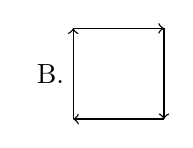
\begin{tikzpicture}[scale=0.72,line width=0.5pt]
\draw[->] (0,0)--(0,1.6);
\draw[->] (0,1.6)--(1.6,1.6);
\draw[->] (1.6,1.6)--(1.6,0);
\draw[->] (1.6,0)--(0,0);
\node at (-0.4,0.8) {B.};
\end{tikzpicture}
&
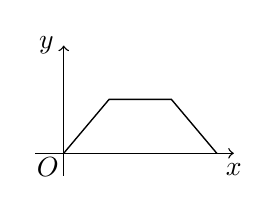
\begin{tikzpicture}[scale=0.72,line width=0.5pt]
\draw[->] (-0.5,0)--(3,0) node[below]{$x$};
\draw[->] (0,-0.4)--(0,1.9) node[left]{$y$};
\draw (0,0)--(0.8,0.95)--(1.9,0.95)--(2.7,0);
\node at (-0.28,-0.25) {$O$};
\end{tikzpicture}
\\
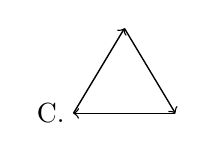
\begin{tikzpicture}[scale=0.72,line width=0.5pt]
\draw[->] (0,0)--(0.9,1.5);
\draw[->] (0.9,1.5)--(1.8,0);
\draw[->] (1.8,0)--(0,0);
\node at (-0.4,0) {C.};
\end{tikzpicture}
&
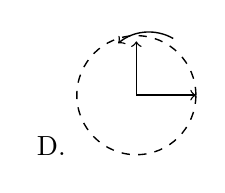
\begin{tikzpicture}[scale=0.72,line width=0.5pt]
\draw[dashed] (1.1,0.9) circle (1.05);
\draw[->] (1.1,0.9)--(2.15,0.9);
\draw[->] (1.1,0.9)--(1.1,1.85);
\draw[->] (1.75,1.9) arc (60:130:0.85);
\node at (-0.4,0) {D.};
\end{tikzpicture}
&
\end{tabular}
\end{center}

\ifanswer
\solbegin
\step{开始离家越来越远，中间离家距离不变，后来离家距离越来越近,}
\step{因此路线 $D$ 符合题意，故选 $D$.}
\solend
\fi

\item 若关于 $x$ 的方程 $ax^2+bx+c=0$（$a>0$）的两个实数根 $x_1$，$x_2$，集合
$S=\{x\mid x>x_1\}$，$T=\{x\mid x>x_2\}$，$P=\{x\mid x<x_1\}$，$Q=\{x\mid x<x_2\}$，则关于 $x$ 的不等式
$ax^2+bx+c>0$ 的解集为\mbox{（\quad）}

\keepwithprev
A. $(S\cap T)\cup(P\cap Q)$\qquad\qquad B. $(S\cap T)\cap(P\cap Q)$

C. $(S\cup T)\cup(P\cup Q)$\qquad\qquad D. $(S\cup T)\cap(P\cup Q)$

\ifanswer
\solbegin
\step{不妨设 $x_1<x_2$，则 $ax^2+bx+c>0$（$a>0$）的解集为 $\{x\mid x<x_1$ 或 $x>x_2\}$,}
\step{$S\cup T=\{x\mid x>x_1\}$，$P\cup Q=\{x\mid x<x_2\}$，$S\cap T=\{x\mid x>x_2\}$,}
\step{$P\cap Q=\{x\mid x<x_1\}$，所以 $(S\cap T)\cup(P\cap Q)=\{x\mid x<x_1$ 或 $x>x_2\}$. 故选 $A$.}
\solend
\fi

\item 已知存在函数 $y=f(x)$ 和 $y=g(x)$ 使得函数 $y=f(g(x))$ 的定义域为 $\R$，且表达式为
$f(g(x))=x^2$，则 $y=g(x)$ 的表达式不可能是\mbox{（\quad）}

\keepwithprev
A. $x^2-3\lvert x\rvert$\qquad B. $x^2+\sqrt{\lvert x\rvert}$\qquad C. $2x-1$\qquad D. $\lvert x\rvert$

\ifanswer
\solbegin
\step{对于选项 A，当 $g(x)=x^2-3\lvert x\rvert$ 时，$g(1)=g(2)=-2$.}
\step{由 $f(g(x))=x^2$ 得 $f(-2)=f(g(1))=1^2=1$，$f(-2)=f(g(2))=2^2=4$，% 原卷两处均作 f(-2)，照录
}
\step{与函数的定义矛盾，所以选项 A 不可能.}
\step{对于选项 B，当 $g(x)=x^2+\sqrt{\lvert x\rvert}$ 时,}
\step{令 $t=x^2+\sqrt{\lvert x\rvert}$，$s=\lvert x\rvert$，$h(s)=s^2+\sqrt s\ (s\geqslant0)$.}
\step{因为函数 $y=s^2$ 在区间 $[0,+\infty)$ 上严格增，函数 $y=\sqrt s$ 在区间 $[0,+\infty)$ 上严格增.}
\step{所以函数 $h(s)=s^2+\sqrt s\ (s\geqslant0)$ 在区间 $[0,+\infty)$ 上严格增.}
\step{故 $s=h^{-1}(t)$，即 $\lvert x\rvert=h^{-1}(t)$，因为 $f(g(x))=x^2=\lvert x\rvert^2$，所以 $f(t)=(h^{-1}(t))^2$,}
\step{即 $f(x)=(h^{-1}(x))^2$，此时 $y=f(g(x))$ 的定义域为 $\R$，故选项 B 可能.}
\step{对于选项 C，当 $g(x)=2x-1$ 时，由 $f(g(x))=x^2$ 得 $f(g(x))=f(2x-1)=x^2$,}
\step{则 $f(x)=\left(\dfrac{x+1}2\right)^2$，此时 $y=f(g(x))$ 的定义域为 $\R$，故选项 C 可能.}
\step{对于选项 D，当 $g(x)=\lvert x\rvert$ 时，由 $f(g(x))=x^2$ 得 $f(g(x))=f(\lvert x\rvert)=x^2$,}
\step{则 $f(x)=x^2\ (x\geqslant0)$，此时 $y=f(g(x))$ 的定义域为 $\R$，故选项 D 可能.}
\step{故选 $A$.}
\solend
\fi

\end{enumerate}

\bigsec{三、解答题}

\begin{enumerate}
\setcounter{enumi}{16}

\item 已知常数 $a\in\R$，集合 $A=\left\{x\,\middle|\,\dfrac{2x+11}{x+2}\geqslant3\right\}$，集合 $B=\{x\mid x^2+2ax-3a^2<0\}$.

（1）若 $a=2$，求 $A\cap B$；

（2）若 $A\cup B=A$，求实数 $a$ 的取值范围.

\ifanswer
\solbegin
\step{（1）$\dfrac{2x+11}{x+2}\geqslant3\Leftrightarrow\dfrac{-x+5}{x+2}\geqslant0\Leftrightarrow\dfrac{x-5}{x+2}\leqslant0\Leftrightarrow
\begin{cases}x+2\neq0\\(x-5)(x+2)\leqslant0\end{cases}$}
\step{$\Leftrightarrow-2<x\leqslant5$，$A=(-2,5]$,}
\step{当 $a=2$ 时，$B=\{x\mid x^2+4x-12<0\}=\{x\mid(x-2)(x+6)<0\}=(-6,2)$,}
\step{$A\cap B=(-2,2)$；}
\step{（2）由 $A\cup B=A$ 得 $B\subseteq A$,}
\step{当 $a=0$ 时，$B=\{x\mid x^2<0\}=\varnothing$，满足题意,}
\step{$x^2+2ax-3a^2=0$ 的两根分别是 $a$ 和 $-3a$,}
\step{当 $a>0$ 时，$B=(-3a,a)$，由题意得 $-2\leqslant-3a<a\leqslant5$，解得 $0<a\leqslant\dfrac23$,}
\step{当 $a<0$ 时，$B=(a,-3a)$，由题意得 $-2\leqslant a<-3a\leqslant5$，解得 $-\dfrac53\leqslant a<0$,}
\step{综上，$-\dfrac53\leqslant a\leqslant\dfrac23$.}
\solend
\fi

\item 某奶茶店今年年初花费 16 万元购买了一台制作冰淇淋的设备，经估算，该设备每年可
为该奶茶店提供 12 万元的总收入. 已知使用 $x$ 年（$x$ 为正整数）所需的各种维护费用总计为
$x^2+2x$ 万元（今年为第一年）.

（1）试问：该奶茶店第几年开始盈利（总收入超过总支出）？

（2）该奶茶店在若干年后要卖出该冰淇淋设备，有以下两种方案：

①当盈利总额达到最大值时，以 1 万元的价格卖出该设备；

②当年均盈利达到最大值时，以 2 万元的价格卖出该设备.

试问哪一种方案较为划算？请说明理由.

\ifanswer
\solbegin
\step{（1）由题意得总收入扣除支出后的纯收入 $y=12x-(x^2+2x+16)$}
\step{$=-x^2+10x-16$，$-x^2+10x-16>0$，解得 $2<x<8$,}
\step{由 $x\in\N^*$，所以从第三年开始盈利；}
\step{（2）方案①：纯收入 $y=-x^2+10x-16=-(x-5)^2+9$,}
\step{则 5 年后盈利总额达到最大值 9 万元，}
\step{以 1 万元的价格卖出该设备，共盈利 10 万元；}
\step{方案②：年均盈利 $z=\dfrac{-x^2+10x-16}{x}=-x+10-\dfrac{16}{x}$,}
\step{由 $x\in\N^*$，$x+\dfrac{16}{x}\geqslant2\sqrt{x\cdot\dfrac{16}{x}}=8$，当且仅当 $x=\dfrac{16}{x}$，即 $x=4$ 时取等号,}
\step{$z=-x+10-\dfrac{16}{x}\leqslant-8+10=2$，当 4 年后年均盈利达到最大值 2 万元时,}
\step{以 2 万元的价格卖出该设备，共盈利 $4\times2+2=10$ 万元.}
\step{两种方案盈利总数一样，但方案②时间短，较为划算.}
\solend
\fi

\item 已知常数 $m\in\R$，$f(x)=\sqrt{\sqrt{x(4-x)}-mx}$.% 原卷题干为双层根号，其解析按单层，见文件头注

（1）证明：对任意的 $m\in\R$，$\{x\mid y=f(x)\}\neq\varnothing$；

（2）若 $[0,2]\subseteq\{x\mid y=f(x)\}$，求实数 $m$ 的取值范围；

（3）若 $\{x\mid y=f(x)\}=[0,3]$，求实数 $m$ 的值.

\ifanswer
\solbegin
\step{（1）$\{x\mid y=f(x)\}=\{x\mid\sqrt{x(4-x)}-mx\geqslant0\}$,}
\step{由 $x(4-x)\geqslant0$ 得 $0\leqslant x\leqslant4$,}
\step{当 $m\leqslant0$ 时，由于 $0\leqslant x\leqslant4$,}
\step{所以 $\sqrt{x(4-x)}-mx\geqslant0$ 对任意 $0\leqslant x\leqslant4$ 恒成立,}
\step{故此时 $\{x\mid y=f(x)\}=\{x\mid0\leqslant x\leqslant4\}$，满足 $\{x\mid y=f(x)\}\neq\varnothing$,}
\step{当 $m>0$ 时，由于 $0\leqslant x\leqslant4$，所以 $mx\geqslant0$，所以 $x(4-x)\geqslant m^2x^2$,}
\step{得 $0\leqslant x\leqslant\dfrac4{1+m^2}$，故此时 $\{x\mid y=f(x)\}=\left\{x\,\middle|\,0\leqslant x\leqslant\dfrac4{1+m^2}\right\}$,}
\step{满足 $\{x\mid y=f(x)\}\neq\varnothing$,}
\step{所以，对任意的 $m\in\R$，$\{x\mid y=f(x)\}\neq\varnothing$；}
\step{（2）由（1）得当 $m\leqslant0$ 时，$\{x\mid y=f(x)\}=\{x\mid0\leqslant x\leqslant4\}$,}
\step{显然满足 $[0,2]\subseteq\{x\mid y=f(x)\}$.}
\step{当 $m>0$ 时，$\{x\mid y=f(x)\}=\left\{x\,\middle|\,0\leqslant x\leqslant\dfrac4{1+m^2}\right\}$,}
\step{由于 $[0,2]\subseteq\{x\mid y=f(x)\}$，所以 $\dfrac4{1+m^2}\geqslant2$，故 $0<m\leqslant1$,}
\step{综上，$m\leqslant1$；}
\step{（3）由于 $\{x\mid y=f(x)\}=[0,3]$,}
\step{所以 $m>0$，$\{x\mid y=f(x)\}=\left\{x\,\middle|\,0\leqslant x\leqslant\dfrac4{1+m^2}\right\}$,}
\step{因此 $\dfrac4{1+m^2}=3$，所以 $m=\dfrac{\sqrt3}3$.}
\solend
\fi

\item 已知函数 $y=f(x)$ 的定义域为 $\R$，其图像是一段连续曲线，对任意的 $a$、$b\in\R$，恒
有 $f(a-b)+f(a+b)=5f(a)\cdot f(b)$，且 $f(0)\neq0$，$f(1)=\dfrac23$.

（1）求 $f(0)$ 和 $f(2)$ 的值；

（2）判断函数 $y=f(x)$ 的奇偶性，并证明；

（3）证明：方程 $f(x)=5$ 在区间 $(2,3)$ 上有解.

\ifanswer
\solbegin
\step{（1）对任意的 $a$、$b\in\R$，恒有 $f(a-b)+f(a+b)=5f(a)\cdot f(b)$,}
\step{且 $f(0)\neq0$，$f(1)=\dfrac23$,}
\step{当 $a=1,b=0$ 时，$f(1)+f(1)=5f(1)\cdot f(0)$，解得 $f(0)=\dfrac25$,}
\step{当 $a=b=1$ 时，$f(0)+f(2)=5f(1)\cdot f(1)$，解得 $f(2)=\dfrac{82}{45}$；}
\step{（2）函数 $y=f(x)$ 为偶函数，证明如下：}
\step{当 $a=0,b=x$ 时，$f(-x)+f(x)=5f(0)\cdot f(x)=2f(x)$,}
\step{则有 $f(-x)=f(x)$，又函数 $y=f(x)$ 的定义域为 $\R$,}
\step{所以函数 $y=f(x)$ 为偶函数.}
\step{（2）$f(2)=\dfrac{82}{45}$% 原卷 (3) 的解答开头误标（2）并重印此行，照录
}
\step{当 $a=2,b=1$ 时，$f(1)+f(3)=5f(2)\cdot f(1)$，解得 $f(3)=\dfrac{146}{27}$,}
\step{函数 $y=f(x)$ 的图像是一段连续曲线，$\dfrac{82}{45}<5<\dfrac{146}{27}$,}
\step{所以存在 $x_0\in(2,3)$，使 $f(x_0)=5$,}
\step{即方程 $f(x)=5$ 在区间 $(2,3)$ 上有解.}
\solend
\fi

\item 若函数 $y=F(x)$ 的定义域为 $D$，且对于任意的 $x_1$、$x_2\in D$，“$F(x_1)=F(x_2)$”的充要
条件是“$x_1=x_2$”，则称函数 $y=F(x)$ 为 $D$ 上的“单值函数”. 对于函数 $y=f(x)$，记
$f^{(1)}(x)=f(x)$，$f^{(2)}(x)=f(f(x))$，$f^{(3)}(x)=f(f(f(x)))$，$\cdots$，$f^{(n+1)}(x)=f(f^{(n)}(x))$，其
中 $n=1,2,3,\cdots$，并对任意的 $A\subseteq D$，记集合 $f^{(n)}(A)=\left\{f^{(n)}(x)\mid x\in A\right\}$，并规定
$f^{(n)}(\varnothing)=\varnothing$.

（1）若 $f(x)=2x+1$，函数 $y=f(x)$ 的定义域为 $\R$，求 $f^{(2)}([0,1])$ 和 $f^{(3)}([0,1])$；

（2）若函数 $y=f(x)$ 的定义域为 $D$，且存在正整数 $m$，使得对任意的 $x\in D$，$f^{(m)}(x)=x$，
求证：函数 $y=f(x)$ 为 $D$ 上的“单值函数”；

（3）设 $a\in(0,1)$，若函数 $y=f(x)$ 的定义域为 $(0,1]$，且表达式为：
\[f(x)=\begin{cases}x+(1-a),&0<x\leqslant a,\\x-a,&a<x\leqslant1\end{cases}\]
判断 $y=f(x)$ 是否为 $(0,1]$ 上的“单值函数”，并证明对任
意的区间 $I\subseteq(0,1]$，存在正整数 $k$，使得 $f^{(k)}(I)\cap I\neq\varnothing$.

\ifanswer
\solbegin
\step{（1）当 $x\in[0,1]$ 时，$2x+1\in[1,3]$，所以 $f^{(1)}([0,1])=[1,3]$,}
\step{当 $x\in[1,3]$ 时，$2x+1\in[3,7]$，所以 $f^{(2)}([0,1])=[3,7]$,}
\step{当 $x\in[3,7]$ 时，$2x+1\in[7,15]$，所以 $f^{(3)}([0,1])=[7,15]$；}
\step{（2）由已知单值函数的定义可以改写为：若函数 $y=F(x)$ 的定义域为 $D$,}
\step{且对于任意的 $x_1$、$x_2\in D$，“$F(x_1)\neq F(x_2)$”的充要条件是“$x_1\neq x_2$”,}
\step{则称函数 $y=F(x)$ 为 $D$ 上的“单值函数.}
\step{假设 $f(x)$ 不是 $D$ 上的单值函数,}
\step{则存在 $x_1,x_2\in D,x_1\neq x_2$，$f(x_1)=f(x_2)$ 成立，即 $f^{(1)}(x_1)=f^{(1)}(x_2)$,}
\step{于是 $f\left[f^{(1)}(x_1)\right]=f\left[f^{(1)}(x_2)\right]$，即 $f^{(2)}(x_1)=f^{(2)}(x_2)$,}
\step{依此类推，得 $f^{(m)}(x_1)=f^{(m)}(x_2)$,}
\step{但由题意得 $f^{(m)}(x)=x$，因此 $f^{(2)}(x_1)=x_2$，$f^{(2)}(x_2)=x_2$，而 $x_1\neq x_2$,}
\step{因此 $f^{(m)}(x_1)\neq f^{(m)}(x_2)$，这样得出了矛盾的结论，所以假设不成立,}
\step{即 $f(x)$ 是 $D$ 上的单值函数；}
\step{（3）由新定义得 $f(x)=x+(1-a)$ 是单值函数，$f(x)=x-a$ 也是单值函数,}
\step{$0<a<1$，则 $0<1-a<1$,}
\step{又 $0<x\leqslant a$ 时，$f(x)=x+(1-a)\in(1-a,1]$,}
\step{$a<x\leqslant1$ 时，$f(x)=x-a\in(0,1-a]$，又 $(0,1-a]\cap(1-a,1]=\varnothing$,}
\step{因此对任意的 $x_1,x_2\in(0,1],x_1\neq x_2\Leftrightarrow f(x_1)\neq f(x_2)$,}
\step{所以 $y=f(x)$ 是 $(0,1]$ 上的“单值函数”,}
\step{对于任意的有限的区间 $I$，记 $\lvert I\rvert$ 表示区间 $I$ 的长度,}
\step{如果一个集合 $A$ 是若干个区间的并集,}
\step{则 $\lvert A\rvert$ 等于组成它的所有区间的长度之和,}
\step{对于任意的区间 $I\subseteq(0,1]$，$x\in I$，$f(I)=\{f(x)\mid x\in T\}$,}
\step{不妨设 $I=(s,t)$，$(0<s<t\leqslant1)$，$\lvert T\rvert=t-s$,}
\step{若 $(s,t)\subseteq(0,a]$，则 $f(I)=(s+1-a,t+1-a)$，$\lvert f(T)\rvert=t-s$,}
\step{若 $(s,t)\subseteq(a,1]$，则 $f(I)=(s-a,t-a)$，$\lvert f(T)\rvert=t-s$,}
\step{若 $a\in(s,t)$，则 $f(I)=(s+1-a,1]\cup(0,t-a)$,}
\step{$\lvert f(T)\rvert=1-(s+1-a)+(t-a)-0=t-s$，所以 $\lvert f(I)\rvert=\lvert I\rvert$,}
\step{对于任意的区间 $I\subseteq(0,1]$，显然存在正整数 $n$，使得 $n\lvert I\rvert>1$,}
\step{因此在 $f^{(0)}(I),f^{(1)}(I),f^{(2)}(I),\cdots,f^{(n)}(I)$（它们的长度和大于 1）中,}
\step{必然存在正整数 $m,l\ (m>l)$，使得 $f^{(m)}(I)\cap f^{(l)}(I)\neq\varnothing$,}
\step{因此必存在 $x,y\in I$，使得 $f^{(m)}(x)=f^{(l)}(y)$,}
\step{又 $y=f(x)$ 是 $(0,1]$ 上的单值函数,}
\step{所以 $f^{(m-1)}(x)=f^{(l-1)}(y)$，$f^{(m-2)}(x)=f^{(l-2)}(y)$，$\cdots$，$f^{(m-l)}(x)=y$,}
\step{这表示 $f^{(m-l)}(I)\cap I\neq\varnothing$，取 $k=m-l$,}
\step{所以对任意的区间 $I\subseteq(0,1]$，存在正整数 $k$，使得 $f^{(k)}(I)\cap I\neq\varnothing$.}
\solend
\fi

\end{enumerate}

\end{document}
"
% 紧凑版：xelatex "\def\iscompact{1}% 高一106_复旦附中_周末作业11期中复习.tex
%   —— 高一上数学“2026-2027 年复旦附中高一上周末作业 11 期中复习”（试卷版/答案版）
% 试卷版：xelatex 高一106_复旦附中_周末作业11期中复习.tex
% 答案版：xelatex "\def\isanswer{1}\input{高一106_复旦附中_周末作业11期中复习.tex}"
% 紧凑版：xelatex "\def\iscompact{1}\input{高一106_复旦附中_周末作业11期中复习.tex}"
%
% 原始材料：微信公众号“魔都数学加油站”文章，作者破晓，2026-11-03 17:19 发布；
% 连载“27学年高一106”，原文标题“27学年高一106——2026-2027年上海市复旦附中高一上周末作业11期中复习”；
% 原文链接：https://mp.weixin.qq.com/s/O3N1S8hA2awUzsOnRvCI-w。
% 正文为 9 张 PNG 页（第 1—2、4—8 页 4762×6735，第 3、9 页 2560×3620），题目下印有【解析】，为讲评版。
% 题目、解析均据原图转录；卷面水印及公众号页脚未录入。
% 第 14 题的四幅路线图选项与题干右侧的 $y$-$x$ 图像按原图形状用 TikZ 重绘。
%
% 卷首标题：原卷印作“2026-2027 年复旦附中高一上周末作业 11 期中复习”（公众号标题中的“上海市”
% 卷面标题行没有，本稿照卷面），年份区间按全稿惯例排 en dash；原卷未印副标题，本稿按题目内容
% 标为“集合与常用逻辑用语、不等式、函数”（期中复习跨三章）。
%
% 与原卷的排版差异：
%   ① 原文从第 3 题起，填空题编号为 3—12、选择题为 13—16、解答题为 17—21，本稿保留原题号；
%   ② 原卷每题下直接印【解析】，本稿按全稿惯例将解析置于答案版；第 13 题原卷把答案“$A$”
%      印在题干括号内且无【解析】，本稿试卷版留空、答案版提 \ans{}；
%   ③ 原卷未印副标题，本稿按“知识模块”口径补出；
%   ④ 原卷填空横线按全稿惯例排为 \blankline[4.4em]；解答题按惯例加 \ansspace；选择题括号排
%      \mbox{（\quad）}、选项段前按惯例加 \keepwithprev；
%   ⑤ 原卷数集排粗体 $\mathbf{R}$，按全稿惯例改 \R；
%   ⑥ 第 11 题题干“集　合　X”三字原卷字距拉得很开（铅字排版的空隙），本稿按正常字距排。
%
% 原卷存疑：第 16 题解析第二行原卷作“$f(-2)=f(g(1))=1^2=1$，$f(-2)=f(g(2))=2^2=4$”
% （两个都写 $f(-2)$；按 $g(1)=g(2)=-2$，两处相等正构成矛盾，但第二处按复合应写
% $f(g(2))=f(-2)$），本稿照录。第 19 题题干 $f(x)$ 为**双层根号**
% $\sqrt{\sqrt{x(4-x)}-mx}$，而解析 (1) 首行只写单层 $\sqrt{x(4-x)}-mx\geqslant0$
% （其后推导均按单层），原卷题干与解析不一致，各照录。
% 第 20 题解析 (3) 的解答开头原卷误标“（2）”并重印 $f(2)=\dfrac{82}{45}$ 一行，照录。
%
% 行数核对：逐题数 \step/\stepm 条数，合计 132 条（Q3：2；Q4：3；Q5：3；Q6：1；Q7：3；
% Q8：5；Q9：2；Q10：2；Q11：3；Q12：2；Q13：0；Q14：2；Q15：3；Q16：14；Q17：10；
% Q18：11；Q19：17；Q20：13；Q21：36），与原卷印刷行逐题相等。第 13 题括号内印答案、
% 无解析，提 \ans{}，不计入 \step 账。
%
\documentclass[a4paper,11pt]{article}
\usepackage{common}

\begin{document}

\examtitlest[3]{2026--2027 年复旦附中高一上周末作业 11 期中复习}{集合与常用逻辑用语、不等式、函数}

\bigsec{一、填空题}

\begin{enumerate}
\setcounter{enumi}{2}

\item 若关于 $x$ 的不等式组
$\begin{cases}2x+3>0\\x+3a<0\end{cases}$
的解集非空，则满足条件的最大整数 $a=$\blankline[4.4em].

\ifanswer
\solbegin
\step{由
$\begin{cases}2x+3>0\\x+3a<0\end{cases}$
得
$\begin{cases}x>-\dfrac32\\x<-3a\end{cases}$，
要使不等式组
$\begin{cases}2x+3>0\\x+3a<0\end{cases}$
的解集非空，}
\step{须 $-3a>-\dfrac32$，即 $a<\dfrac12$，故满足条件的最大整数 $a=0$.}
\solend
\fi

\item 若关于 $x$ 的不等式 $\lvert x-366\rvert+\lvert x-500\rvert\leqslant a$ 的解集非空，则 $a$ 的取值范围是\blankline[4.4em].

\ifanswer
\solbegin
\step{$\lvert x-366\rvert+\lvert x-500\rvert\geqslant\lvert x-366-(x-500)\rvert=134$,}
\step{当且仅当 $366\leqslant x\leqslant500$ 时取等号，所以 $\lvert x-366\rvert+\lvert x-500\rvert$ 的最小值为 134,}
\step{从而 $a\geqslant134$. 故 $a$ 的取值范围是 $[134,+\infty)$.}
\solend
\fi

\item 设集合 $A=\{1,2,3,4\}$，$B=\{1,2\}$，若 $C\subseteq A$ 且 $B\cap C\neq\varnothing$，则所有满足条件的集合 $C$ 的个数为\blankline[4.4em].

\ifanswer
\solbegin
\step{按题意，集合 $C$ 是 $A$ 的子集，且与 $B$ 的交集不为空集,}
\step{集合 $A$ 的子集有 $2^4=16$ 个，其中与 $B$ 的交集为空集的子集，即 $\{3,4\}$ 的子集,}
\step{有 $2^2=4$ 个，故满足题意的集合 $C$ 的个数为 $16-4=12$.}
\solend
\fi

\item 函数 $f(x)=\lvert x^2-3x+2\rvert$ 的单调增区间为\blankline[4.4em].

\ifanswer
\solbegin
\step{观察图像得函数 $f(x)=\lvert x^2-3x+2\rvert$ 的严格增区间为 $\left(1,\dfrac32\right),(2,+\infty)$.}
\solend
\fi

\item 已知 $f(x)=\sqrt{mx^2-mx+1}$，若函数 $y=f(x)$ 的定义域为 $\R$，则实数 $m$ 的取值范围为\blankline[4.4em].

\ifanswer
\solbegin
\step{当 $m=0$ 时，$f(x)=1$ 满足题意,}
\step{当 $m>0$ 时，$\Delta=m^2-4m\leqslant0$，所以 $0<m\leqslant4$,}
\step{故实数 $m$ 的取值范围为 $[0,4]$.}
\solend
\fi

\item 已知 $T$ 是方程 $x^2+px+q=0$（$p^2-4q>0$）的解集，$A=\{1,3,5,7,9\}$，$B=\{1,4,7,10\}$ 且 $T\cap A=\varnothing$，$T\cap B=T$，则 $p+q=$\blankline[4.4em].

\ifanswer
\solbegin
\step{对方程 $x^2+px+q=0$（$p^2-4q>0$），显然有两个根，故集合 $T$ 中有两个元素；}
\step{因为 $T\cap B=T$，所以 $T$ 中的两个元素一定在集合 $B$ 中；}
\step{又因为 $T\cap A=\varnothing$，故 $T$ 中的所有元素都不在 $A$ 中；}
\step{综上，$T$ 中的元素一定是 4 和 10，由根与系数的关系得 $14=-p,40=q$,}
\step{则 $p+q=26$.}
\solend
\fi

\item 已知正实数 $a$、$b$ 满足 $a+b=a^2+b^2$，则 $\dfrac1a+\dfrac1b$ 的最小值为\blankline[4.4em].

\ifanswer
\solbegin
\step{由已知 $\dfrac1a+\dfrac1b=\dfrac{a+b}{ab}=\dfrac{a^2+b^2}{ab}=\dfrac ab+\dfrac ba\geqslant2\sqrt{\dfrac ab\cdot\dfrac ba}=2$,}
\step{当且仅当 $\dfrac ba=\dfrac ab$，即 $a=b=1$ 时取等号，故 $\dfrac1a+\dfrac1b$ 的最小值为 $1$.}
\solend
\fi

\item 已知 $a$、$b$、$c$ 为实数，且 $a^2+c^2=64$，$b^2+c^2=100$，则 $a^2+b^2$ 的取值范围是\blankline[4.4em].

\ifanswer
\solbegin
\step{由题意得
$\begin{cases}a^2=64-c^2\\b^2=100-c^2\end{cases}\Rightarrow a^2+b^2=164-2c^2$，
其中 $0\leqslant c^2\leqslant64$,}
\step{因此 $a^2+b^2$ 的取值范围是 $[36,164]$.}
\solend
\fi

\item 设 $U$ 为全集，对集合 $X$，$Y$，定义运算“$*$”，$M*N=\overline{M\cap N}$. 已知全集
$U=\{1,2,3,4,5,6,7,8\}$，集合 $X=\{1,2,3\}$，$Y=\{3,4,5\}$，$Z=\{2,4,7\}$，则
$(X*Y)*Z=$\blankline[4.4em].% 原卷“集 合 X”三字字距拉得很开，本稿按正常字距排

\ifanswer
\solbegin
\step{因为集合 $U=\{1,2,3,4,5,6,7,8\}$，$X=\{1,2,3\}$，$Y=\{3,4,5\}$，$Z=\{2,4,7\}$,}
\step{所以 $X\cap Y=\{3\}$，则 $X*Y=\overline{X\cap Y}=\{1,2,4,5,6,7,8\}$,}
\step{又 $\{1,2,4,5,6,7,8\}\cap\{2,4,7\}=\{2,4,7\}$，所以 $(X*Y)*Z=\{1,3,5,6,8\}$.}
\solend
\fi

\item 已知一个奇函数 $y=f(x)$ 与一个偶函数 $y=g(x)$ 的和为函数 $y=\sqrt{x^2-3x+6}$，则 $f(3)=$\blankline[4.4em].

\ifanswer
\solbegin
\step{记 $h(x)=\sqrt{x^2-3x+6}$，由题意得
$\begin{cases}f(3)+g(3)=h(3)=\sqrt6\\f(-3)+g(-3)=h(-3)=2\sqrt6\end{cases}$,}
\step{又 $f(-3)=-f(3)$，$g(-3)=g(3)$，解得 $f(3)=-\dfrac{\sqrt6}2$.}
\solend
\fi

\end{enumerate}

\bigsec{二、选择题}

\begin{enumerate}
\setcounter{enumi}{12}

\item 已知 $a>b$ 均为正实数，则“$c>d$”是“$a+c>b+d$”的\mbox{（\quad）}条件% 原卷把答案“A”印在题干括号内、无【解析】

\keepwithprev
A. 充分非必要\qquad\qquad B. 必要不充分

C. 充分必要\qquad\qquad\qquad D. 既非充分又非必要

\ifanswer
\ans{$A$}
\fi

\item 如图是肖老师以恒定的速率夜跑时的离家距离 $(y)$ 与跑步时间 $(x)$ 之间的函数的图像，
则肖老师跑步的路线可能是\mbox{（\quad）}

\keepwithprev
\begin{center}
\begin{tabular}{ccc}
\begin{tikzpicture}[scale=0.72,line width=0.5pt]
\draw[->] (0,0)--(1.1,1.1);
\draw[->] (1.1,1.1)--(2.7,1.1);
\draw[->] (2.7,1.1)--(3.8,0);
\node at (-0.4,0) {A.};
\end{tikzpicture}
&
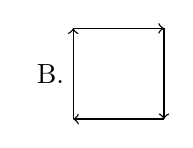
\begin{tikzpicture}[scale=0.72,line width=0.5pt]
\draw[->] (0,0)--(0,1.6);
\draw[->] (0,1.6)--(1.6,1.6);
\draw[->] (1.6,1.6)--(1.6,0);
\draw[->] (1.6,0)--(0,0);
\node at (-0.4,0.8) {B.};
\end{tikzpicture}
&
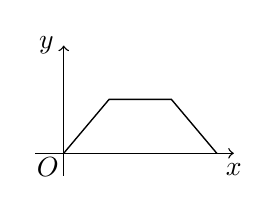
\begin{tikzpicture}[scale=0.72,line width=0.5pt]
\draw[->] (-0.5,0)--(3,0) node[below]{$x$};
\draw[->] (0,-0.4)--(0,1.9) node[left]{$y$};
\draw (0,0)--(0.8,0.95)--(1.9,0.95)--(2.7,0);
\node at (-0.28,-0.25) {$O$};
\end{tikzpicture}
\\
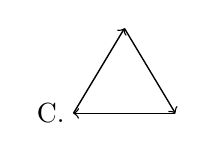
\begin{tikzpicture}[scale=0.72,line width=0.5pt]
\draw[->] (0,0)--(0.9,1.5);
\draw[->] (0.9,1.5)--(1.8,0);
\draw[->] (1.8,0)--(0,0);
\node at (-0.4,0) {C.};
\end{tikzpicture}
&
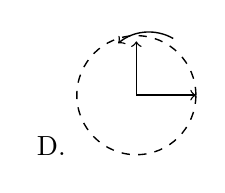
\begin{tikzpicture}[scale=0.72,line width=0.5pt]
\draw[dashed] (1.1,0.9) circle (1.05);
\draw[->] (1.1,0.9)--(2.15,0.9);
\draw[->] (1.1,0.9)--(1.1,1.85);
\draw[->] (1.75,1.9) arc (60:130:0.85);
\node at (-0.4,0) {D.};
\end{tikzpicture}
&
\end{tabular}
\end{center}

\ifanswer
\solbegin
\step{开始离家越来越远，中间离家距离不变，后来离家距离越来越近,}
\step{因此路线 $D$ 符合题意，故选 $D$.}
\solend
\fi

\item 若关于 $x$ 的方程 $ax^2+bx+c=0$（$a>0$）的两个实数根 $x_1$，$x_2$，集合
$S=\{x\mid x>x_1\}$，$T=\{x\mid x>x_2\}$，$P=\{x\mid x<x_1\}$，$Q=\{x\mid x<x_2\}$，则关于 $x$ 的不等式
$ax^2+bx+c>0$ 的解集为\mbox{（\quad）}

\keepwithprev
A. $(S\cap T)\cup(P\cap Q)$\qquad\qquad B. $(S\cap T)\cap(P\cap Q)$

C. $(S\cup T)\cup(P\cup Q)$\qquad\qquad D. $(S\cup T)\cap(P\cup Q)$

\ifanswer
\solbegin
\step{不妨设 $x_1<x_2$，则 $ax^2+bx+c>0$（$a>0$）的解集为 $\{x\mid x<x_1$ 或 $x>x_2\}$,}
\step{$S\cup T=\{x\mid x>x_1\}$，$P\cup Q=\{x\mid x<x_2\}$，$S\cap T=\{x\mid x>x_2\}$,}
\step{$P\cap Q=\{x\mid x<x_1\}$，所以 $(S\cap T)\cup(P\cap Q)=\{x\mid x<x_1$ 或 $x>x_2\}$. 故选 $A$.}
\solend
\fi

\item 已知存在函数 $y=f(x)$ 和 $y=g(x)$ 使得函数 $y=f(g(x))$ 的定义域为 $\R$，且表达式为
$f(g(x))=x^2$，则 $y=g(x)$ 的表达式不可能是\mbox{（\quad）}

\keepwithprev
A. $x^2-3\lvert x\rvert$\qquad B. $x^2+\sqrt{\lvert x\rvert}$\qquad C. $2x-1$\qquad D. $\lvert x\rvert$

\ifanswer
\solbegin
\step{对于选项 A，当 $g(x)=x^2-3\lvert x\rvert$ 时，$g(1)=g(2)=-2$.}
\step{由 $f(g(x))=x^2$ 得 $f(-2)=f(g(1))=1^2=1$，$f(-2)=f(g(2))=2^2=4$，% 原卷两处均作 f(-2)，照录
}
\step{与函数的定义矛盾，所以选项 A 不可能.}
\step{对于选项 B，当 $g(x)=x^2+\sqrt{\lvert x\rvert}$ 时,}
\step{令 $t=x^2+\sqrt{\lvert x\rvert}$，$s=\lvert x\rvert$，$h(s)=s^2+\sqrt s\ (s\geqslant0)$.}
\step{因为函数 $y=s^2$ 在区间 $[0,+\infty)$ 上严格增，函数 $y=\sqrt s$ 在区间 $[0,+\infty)$ 上严格增.}
\step{所以函数 $h(s)=s^2+\sqrt s\ (s\geqslant0)$ 在区间 $[0,+\infty)$ 上严格增.}
\step{故 $s=h^{-1}(t)$，即 $\lvert x\rvert=h^{-1}(t)$，因为 $f(g(x))=x^2=\lvert x\rvert^2$，所以 $f(t)=(h^{-1}(t))^2$,}
\step{即 $f(x)=(h^{-1}(x))^2$，此时 $y=f(g(x))$ 的定义域为 $\R$，故选项 B 可能.}
\step{对于选项 C，当 $g(x)=2x-1$ 时，由 $f(g(x))=x^2$ 得 $f(g(x))=f(2x-1)=x^2$,}
\step{则 $f(x)=\left(\dfrac{x+1}2\right)^2$，此时 $y=f(g(x))$ 的定义域为 $\R$，故选项 C 可能.}
\step{对于选项 D，当 $g(x)=\lvert x\rvert$ 时，由 $f(g(x))=x^2$ 得 $f(g(x))=f(\lvert x\rvert)=x^2$,}
\step{则 $f(x)=x^2\ (x\geqslant0)$，此时 $y=f(g(x))$ 的定义域为 $\R$，故选项 D 可能.}
\step{故选 $A$.}
\solend
\fi

\end{enumerate}

\bigsec{三、解答题}

\begin{enumerate}
\setcounter{enumi}{16}

\item 已知常数 $a\in\R$，集合 $A=\left\{x\,\middle|\,\dfrac{2x+11}{x+2}\geqslant3\right\}$，集合 $B=\{x\mid x^2+2ax-3a^2<0\}$.

（1）若 $a=2$，求 $A\cap B$；

（2）若 $A\cup B=A$，求实数 $a$ 的取值范围.

\ifanswer
\solbegin
\step{（1）$\dfrac{2x+11}{x+2}\geqslant3\Leftrightarrow\dfrac{-x+5}{x+2}\geqslant0\Leftrightarrow\dfrac{x-5}{x+2}\leqslant0\Leftrightarrow
\begin{cases}x+2\neq0\\(x-5)(x+2)\leqslant0\end{cases}$}
\step{$\Leftrightarrow-2<x\leqslant5$，$A=(-2,5]$,}
\step{当 $a=2$ 时，$B=\{x\mid x^2+4x-12<0\}=\{x\mid(x-2)(x+6)<0\}=(-6,2)$,}
\step{$A\cap B=(-2,2)$；}
\step{（2）由 $A\cup B=A$ 得 $B\subseteq A$,}
\step{当 $a=0$ 时，$B=\{x\mid x^2<0\}=\varnothing$，满足题意,}
\step{$x^2+2ax-3a^2=0$ 的两根分别是 $a$ 和 $-3a$,}
\step{当 $a>0$ 时，$B=(-3a,a)$，由题意得 $-2\leqslant-3a<a\leqslant5$，解得 $0<a\leqslant\dfrac23$,}
\step{当 $a<0$ 时，$B=(a,-3a)$，由题意得 $-2\leqslant a<-3a\leqslant5$，解得 $-\dfrac53\leqslant a<0$,}
\step{综上，$-\dfrac53\leqslant a\leqslant\dfrac23$.}
\solend
\fi

\item 某奶茶店今年年初花费 16 万元购买了一台制作冰淇淋的设备，经估算，该设备每年可
为该奶茶店提供 12 万元的总收入. 已知使用 $x$ 年（$x$ 为正整数）所需的各种维护费用总计为
$x^2+2x$ 万元（今年为第一年）.

（1）试问：该奶茶店第几年开始盈利（总收入超过总支出）？

（2）该奶茶店在若干年后要卖出该冰淇淋设备，有以下两种方案：

①当盈利总额达到最大值时，以 1 万元的价格卖出该设备；

②当年均盈利达到最大值时，以 2 万元的价格卖出该设备.

试问哪一种方案较为划算？请说明理由.

\ifanswer
\solbegin
\step{（1）由题意得总收入扣除支出后的纯收入 $y=12x-(x^2+2x+16)$}
\step{$=-x^2+10x-16$，$-x^2+10x-16>0$，解得 $2<x<8$,}
\step{由 $x\in\N^*$，所以从第三年开始盈利；}
\step{（2）方案①：纯收入 $y=-x^2+10x-16=-(x-5)^2+9$,}
\step{则 5 年后盈利总额达到最大值 9 万元，}
\step{以 1 万元的价格卖出该设备，共盈利 10 万元；}
\step{方案②：年均盈利 $z=\dfrac{-x^2+10x-16}{x}=-x+10-\dfrac{16}{x}$,}
\step{由 $x\in\N^*$，$x+\dfrac{16}{x}\geqslant2\sqrt{x\cdot\dfrac{16}{x}}=8$，当且仅当 $x=\dfrac{16}{x}$，即 $x=4$ 时取等号,}
\step{$z=-x+10-\dfrac{16}{x}\leqslant-8+10=2$，当 4 年后年均盈利达到最大值 2 万元时,}
\step{以 2 万元的价格卖出该设备，共盈利 $4\times2+2=10$ 万元.}
\step{两种方案盈利总数一样，但方案②时间短，较为划算.}
\solend
\fi

\item 已知常数 $m\in\R$，$f(x)=\sqrt{\sqrt{x(4-x)}-mx}$.% 原卷题干为双层根号，其解析按单层，见文件头注

（1）证明：对任意的 $m\in\R$，$\{x\mid y=f(x)\}\neq\varnothing$；

（2）若 $[0,2]\subseteq\{x\mid y=f(x)\}$，求实数 $m$ 的取值范围；

（3）若 $\{x\mid y=f(x)\}=[0,3]$，求实数 $m$ 的值.

\ifanswer
\solbegin
\step{（1）$\{x\mid y=f(x)\}=\{x\mid\sqrt{x(4-x)}-mx\geqslant0\}$,}
\step{由 $x(4-x)\geqslant0$ 得 $0\leqslant x\leqslant4$,}
\step{当 $m\leqslant0$ 时，由于 $0\leqslant x\leqslant4$,}
\step{所以 $\sqrt{x(4-x)}-mx\geqslant0$ 对任意 $0\leqslant x\leqslant4$ 恒成立,}
\step{故此时 $\{x\mid y=f(x)\}=\{x\mid0\leqslant x\leqslant4\}$，满足 $\{x\mid y=f(x)\}\neq\varnothing$,}
\step{当 $m>0$ 时，由于 $0\leqslant x\leqslant4$，所以 $mx\geqslant0$，所以 $x(4-x)\geqslant m^2x^2$,}
\step{得 $0\leqslant x\leqslant\dfrac4{1+m^2}$，故此时 $\{x\mid y=f(x)\}=\left\{x\,\middle|\,0\leqslant x\leqslant\dfrac4{1+m^2}\right\}$,}
\step{满足 $\{x\mid y=f(x)\}\neq\varnothing$,}
\step{所以，对任意的 $m\in\R$，$\{x\mid y=f(x)\}\neq\varnothing$；}
\step{（2）由（1）得当 $m\leqslant0$ 时，$\{x\mid y=f(x)\}=\{x\mid0\leqslant x\leqslant4\}$,}
\step{显然满足 $[0,2]\subseteq\{x\mid y=f(x)\}$.}
\step{当 $m>0$ 时，$\{x\mid y=f(x)\}=\left\{x\,\middle|\,0\leqslant x\leqslant\dfrac4{1+m^2}\right\}$,}
\step{由于 $[0,2]\subseteq\{x\mid y=f(x)\}$，所以 $\dfrac4{1+m^2}\geqslant2$，故 $0<m\leqslant1$,}
\step{综上，$m\leqslant1$；}
\step{（3）由于 $\{x\mid y=f(x)\}=[0,3]$,}
\step{所以 $m>0$，$\{x\mid y=f(x)\}=\left\{x\,\middle|\,0\leqslant x\leqslant\dfrac4{1+m^2}\right\}$,}
\step{因此 $\dfrac4{1+m^2}=3$，所以 $m=\dfrac{\sqrt3}3$.}
\solend
\fi

\item 已知函数 $y=f(x)$ 的定义域为 $\R$，其图像是一段连续曲线，对任意的 $a$、$b\in\R$，恒
有 $f(a-b)+f(a+b)=5f(a)\cdot f(b)$，且 $f(0)\neq0$，$f(1)=\dfrac23$.

（1）求 $f(0)$ 和 $f(2)$ 的值；

（2）判断函数 $y=f(x)$ 的奇偶性，并证明；

（3）证明：方程 $f(x)=5$ 在区间 $(2,3)$ 上有解.

\ifanswer
\solbegin
\step{（1）对任意的 $a$、$b\in\R$，恒有 $f(a-b)+f(a+b)=5f(a)\cdot f(b)$,}
\step{且 $f(0)\neq0$，$f(1)=\dfrac23$,}
\step{当 $a=1,b=0$ 时，$f(1)+f(1)=5f(1)\cdot f(0)$，解得 $f(0)=\dfrac25$,}
\step{当 $a=b=1$ 时，$f(0)+f(2)=5f(1)\cdot f(1)$，解得 $f(2)=\dfrac{82}{45}$；}
\step{（2）函数 $y=f(x)$ 为偶函数，证明如下：}
\step{当 $a=0,b=x$ 时，$f(-x)+f(x)=5f(0)\cdot f(x)=2f(x)$,}
\step{则有 $f(-x)=f(x)$，又函数 $y=f(x)$ 的定义域为 $\R$,}
\step{所以函数 $y=f(x)$ 为偶函数.}
\step{（2）$f(2)=\dfrac{82}{45}$% 原卷 (3) 的解答开头误标（2）并重印此行，照录
}
\step{当 $a=2,b=1$ 时，$f(1)+f(3)=5f(2)\cdot f(1)$，解得 $f(3)=\dfrac{146}{27}$,}
\step{函数 $y=f(x)$ 的图像是一段连续曲线，$\dfrac{82}{45}<5<\dfrac{146}{27}$,}
\step{所以存在 $x_0\in(2,3)$，使 $f(x_0)=5$,}
\step{即方程 $f(x)=5$ 在区间 $(2,3)$ 上有解.}
\solend
\fi

\item 若函数 $y=F(x)$ 的定义域为 $D$，且对于任意的 $x_1$、$x_2\in D$，“$F(x_1)=F(x_2)$”的充要
条件是“$x_1=x_2$”，则称函数 $y=F(x)$ 为 $D$ 上的“单值函数”. 对于函数 $y=f(x)$，记
$f^{(1)}(x)=f(x)$，$f^{(2)}(x)=f(f(x))$，$f^{(3)}(x)=f(f(f(x)))$，$\cdots$，$f^{(n+1)}(x)=f(f^{(n)}(x))$，其
中 $n=1,2,3,\cdots$，并对任意的 $A\subseteq D$，记集合 $f^{(n)}(A)=\left\{f^{(n)}(x)\mid x\in A\right\}$，并规定
$f^{(n)}(\varnothing)=\varnothing$.

（1）若 $f(x)=2x+1$，函数 $y=f(x)$ 的定义域为 $\R$，求 $f^{(2)}([0,1])$ 和 $f^{(3)}([0,1])$；

（2）若函数 $y=f(x)$ 的定义域为 $D$，且存在正整数 $m$，使得对任意的 $x\in D$，$f^{(m)}(x)=x$，
求证：函数 $y=f(x)$ 为 $D$ 上的“单值函数”；

（3）设 $a\in(0,1)$，若函数 $y=f(x)$ 的定义域为 $(0,1]$，且表达式为：
\[f(x)=\begin{cases}x+(1-a),&0<x\leqslant a,\\x-a,&a<x\leqslant1\end{cases}\]
判断 $y=f(x)$ 是否为 $(0,1]$ 上的“单值函数”，并证明对任
意的区间 $I\subseteq(0,1]$，存在正整数 $k$，使得 $f^{(k)}(I)\cap I\neq\varnothing$.

\ifanswer
\solbegin
\step{（1）当 $x\in[0,1]$ 时，$2x+1\in[1,3]$，所以 $f^{(1)}([0,1])=[1,3]$,}
\step{当 $x\in[1,3]$ 时，$2x+1\in[3,7]$，所以 $f^{(2)}([0,1])=[3,7]$,}
\step{当 $x\in[3,7]$ 时，$2x+1\in[7,15]$，所以 $f^{(3)}([0,1])=[7,15]$；}
\step{（2）由已知单值函数的定义可以改写为：若函数 $y=F(x)$ 的定义域为 $D$,}
\step{且对于任意的 $x_1$、$x_2\in D$，“$F(x_1)\neq F(x_2)$”的充要条件是“$x_1\neq x_2$”,}
\step{则称函数 $y=F(x)$ 为 $D$ 上的“单值函数.}
\step{假设 $f(x)$ 不是 $D$ 上的单值函数,}
\step{则存在 $x_1,x_2\in D,x_1\neq x_2$，$f(x_1)=f(x_2)$ 成立，即 $f^{(1)}(x_1)=f^{(1)}(x_2)$,}
\step{于是 $f\left[f^{(1)}(x_1)\right]=f\left[f^{(1)}(x_2)\right]$，即 $f^{(2)}(x_1)=f^{(2)}(x_2)$,}
\step{依此类推，得 $f^{(m)}(x_1)=f^{(m)}(x_2)$,}
\step{但由题意得 $f^{(m)}(x)=x$，因此 $f^{(2)}(x_1)=x_2$，$f^{(2)}(x_2)=x_2$，而 $x_1\neq x_2$,}
\step{因此 $f^{(m)}(x_1)\neq f^{(m)}(x_2)$，这样得出了矛盾的结论，所以假设不成立,}
\step{即 $f(x)$ 是 $D$ 上的单值函数；}
\step{（3）由新定义得 $f(x)=x+(1-a)$ 是单值函数，$f(x)=x-a$ 也是单值函数,}
\step{$0<a<1$，则 $0<1-a<1$,}
\step{又 $0<x\leqslant a$ 时，$f(x)=x+(1-a)\in(1-a,1]$,}
\step{$a<x\leqslant1$ 时，$f(x)=x-a\in(0,1-a]$，又 $(0,1-a]\cap(1-a,1]=\varnothing$,}
\step{因此对任意的 $x_1,x_2\in(0,1],x_1\neq x_2\Leftrightarrow f(x_1)\neq f(x_2)$,}
\step{所以 $y=f(x)$ 是 $(0,1]$ 上的“单值函数”,}
\step{对于任意的有限的区间 $I$，记 $\lvert I\rvert$ 表示区间 $I$ 的长度,}
\step{如果一个集合 $A$ 是若干个区间的并集,}
\step{则 $\lvert A\rvert$ 等于组成它的所有区间的长度之和,}
\step{对于任意的区间 $I\subseteq(0,1]$，$x\in I$，$f(I)=\{f(x)\mid x\in T\}$,}
\step{不妨设 $I=(s,t)$，$(0<s<t\leqslant1)$，$\lvert T\rvert=t-s$,}
\step{若 $(s,t)\subseteq(0,a]$，则 $f(I)=(s+1-a,t+1-a)$，$\lvert f(T)\rvert=t-s$,}
\step{若 $(s,t)\subseteq(a,1]$，则 $f(I)=(s-a,t-a)$，$\lvert f(T)\rvert=t-s$,}
\step{若 $a\in(s,t)$，则 $f(I)=(s+1-a,1]\cup(0,t-a)$,}
\step{$\lvert f(T)\rvert=1-(s+1-a)+(t-a)-0=t-s$，所以 $\lvert f(I)\rvert=\lvert I\rvert$,}
\step{对于任意的区间 $I\subseteq(0,1]$，显然存在正整数 $n$，使得 $n\lvert I\rvert>1$,}
\step{因此在 $f^{(0)}(I),f^{(1)}(I),f^{(2)}(I),\cdots,f^{(n)}(I)$（它们的长度和大于 1）中,}
\step{必然存在正整数 $m,l\ (m>l)$，使得 $f^{(m)}(I)\cap f^{(l)}(I)\neq\varnothing$,}
\step{因此必存在 $x,y\in I$，使得 $f^{(m)}(x)=f^{(l)}(y)$,}
\step{又 $y=f(x)$ 是 $(0,1]$ 上的单值函数,}
\step{所以 $f^{(m-1)}(x)=f^{(l-1)}(y)$，$f^{(m-2)}(x)=f^{(l-2)}(y)$，$\cdots$，$f^{(m-l)}(x)=y$,}
\step{这表示 $f^{(m-l)}(I)\cap I\neq\varnothing$，取 $k=m-l$,}
\step{所以对任意的区间 $I\subseteq(0,1]$，存在正整数 $k$，使得 $f^{(k)}(I)\cap I\neq\varnothing$.}
\solend
\fi

\end{enumerate}

\end{document}
"
%
% 原始材料：微信公众号“魔都数学加油站”文章，作者破晓，2026-11-03 17:19 发布；
% 连载“27学年高一106”，原文标题“27学年高一106——2026-2027年上海市复旦附中高一上周末作业11期中复习”；
% 原文链接：https://mp.weixin.qq.com/s/O3N1S8hA2awUzsOnRvCI-w。
% 正文为 9 张 PNG 页（第 1—2、4—8 页 4762×6735，第 3、9 页 2560×3620），题目下印有【解析】，为讲评版。
% 题目、解析均据原图转录；卷面水印及公众号页脚未录入。
% 第 14 题的四幅路线图选项与题干右侧的 $y$-$x$ 图像按原图形状用 TikZ 重绘。
%
% 卷首标题：原卷印作“2026-2027 年复旦附中高一上周末作业 11 期中复习”（公众号标题中的“上海市”
% 卷面标题行没有，本稿照卷面），年份区间按全稿惯例排 en dash；原卷未印副标题，本稿按题目内容
% 标为“集合与常用逻辑用语、不等式、函数”（期中复习跨三章）。
%
% 与原卷的排版差异：
%   ① 原文从第 3 题起，填空题编号为 3—12、选择题为 13—16、解答题为 17—21，本稿保留原题号；
%   ② 原卷每题下直接印【解析】，本稿按全稿惯例将解析置于答案版；第 13 题原卷把答案“$A$”
%      印在题干括号内且无【解析】，本稿试卷版留空、答案版提 \ans{}；
%   ③ 原卷未印副标题，本稿按“知识模块”口径补出；
%   ④ 原卷填空横线按全稿惯例排为 \blankline[4.4em]；解答题按惯例加 \ansspace；选择题括号排
%      \mbox{（\quad）}、选项段前按惯例加 \keepwithprev；
%   ⑤ 原卷数集排粗体 $\mathbf{R}$，按全稿惯例改 \R；
%   ⑥ 第 11 题题干“集　合　X”三字原卷字距拉得很开（铅字排版的空隙），本稿按正常字距排。
%
% 原卷存疑：第 16 题解析第二行原卷作“$f(-2)=f(g(1))=1^2=1$，$f(-2)=f(g(2))=2^2=4$”
% （两个都写 $f(-2)$；按 $g(1)=g(2)=-2$，两处相等正构成矛盾，但第二处按复合应写
% $f(g(2))=f(-2)$），本稿照录。第 19 题题干 $f(x)$ 为**双层根号**
% $\sqrt{\sqrt{x(4-x)}-mx}$，而解析 (1) 首行只写单层 $\sqrt{x(4-x)}-mx\geqslant0$
% （其后推导均按单层），原卷题干与解析不一致，各照录。
% 第 20 题解析 (3) 的解答开头原卷误标“（2）”并重印 $f(2)=\dfrac{82}{45}$ 一行，照录。
%
% 行数核对：逐题数 \step/\stepm 条数，合计 132 条（Q3：2；Q4：3；Q5：3；Q6：1；Q7：3；
% Q8：5；Q9：2；Q10：2；Q11：3；Q12：2；Q13：0；Q14：2；Q15：3；Q16：14；Q17：10；
% Q18：11；Q19：17；Q20：13；Q21：36），与原卷印刷行逐题相等。第 13 题括号内印答案、
% 无解析，提 \ans{}，不计入 \step 账。
%
\documentclass[a4paper,11pt]{article}
\usepackage{common}

\begin{document}

\examtitlest[3]{2026--2027 年复旦附中高一上周末作业 11 期中复习}{集合与常用逻辑用语、不等式、函数}

\bigsec{一、填空题}

\begin{enumerate}
\setcounter{enumi}{2}

\item 若关于 $x$ 的不等式组
$\begin{cases}2x+3>0\\x+3a<0\end{cases}$
的解集非空，则满足条件的最大整数 $a=$\blankline[4.4em].

\ifanswer
\solbegin
\step{由
$\begin{cases}2x+3>0\\x+3a<0\end{cases}$
得
$\begin{cases}x>-\dfrac32\\x<-3a\end{cases}$，
要使不等式组
$\begin{cases}2x+3>0\\x+3a<0\end{cases}$
的解集非空，}
\step{须 $-3a>-\dfrac32$，即 $a<\dfrac12$，故满足条件的最大整数 $a=0$.}
\solend
\fi

\item 若关于 $x$ 的不等式 $\lvert x-366\rvert+\lvert x-500\rvert\leqslant a$ 的解集非空，则 $a$ 的取值范围是\blankline[4.4em].

\ifanswer
\solbegin
\step{$\lvert x-366\rvert+\lvert x-500\rvert\geqslant\lvert x-366-(x-500)\rvert=134$,}
\step{当且仅当 $366\leqslant x\leqslant500$ 时取等号，所以 $\lvert x-366\rvert+\lvert x-500\rvert$ 的最小值为 134,}
\step{从而 $a\geqslant134$. 故 $a$ 的取值范围是 $[134,+\infty)$.}
\solend
\fi

\item 设集合 $A=\{1,2,3,4\}$，$B=\{1,2\}$，若 $C\subseteq A$ 且 $B\cap C\neq\varnothing$，则所有满足条件的集合 $C$ 的个数为\blankline[4.4em].

\ifanswer
\solbegin
\step{按题意，集合 $C$ 是 $A$ 的子集，且与 $B$ 的交集不为空集,}
\step{集合 $A$ 的子集有 $2^4=16$ 个，其中与 $B$ 的交集为空集的子集，即 $\{3,4\}$ 的子集,}
\step{有 $2^2=4$ 个，故满足题意的集合 $C$ 的个数为 $16-4=12$.}
\solend
\fi

\item 函数 $f(x)=\lvert x^2-3x+2\rvert$ 的单调增区间为\blankline[4.4em].

\ifanswer
\solbegin
\step{观察图像得函数 $f(x)=\lvert x^2-3x+2\rvert$ 的严格增区间为 $\left(1,\dfrac32\right),(2,+\infty)$.}
\solend
\fi

\item 已知 $f(x)=\sqrt{mx^2-mx+1}$，若函数 $y=f(x)$ 的定义域为 $\R$，则实数 $m$ 的取值范围为\blankline[4.4em].

\ifanswer
\solbegin
\step{当 $m=0$ 时，$f(x)=1$ 满足题意,}
\step{当 $m>0$ 时，$\Delta=m^2-4m\leqslant0$，所以 $0<m\leqslant4$,}
\step{故实数 $m$ 的取值范围为 $[0,4]$.}
\solend
\fi

\item 已知 $T$ 是方程 $x^2+px+q=0$（$p^2-4q>0$）的解集，$A=\{1,3,5,7,9\}$，$B=\{1,4,7,10\}$ 且 $T\cap A=\varnothing$，$T\cap B=T$，则 $p+q=$\blankline[4.4em].

\ifanswer
\solbegin
\step{对方程 $x^2+px+q=0$（$p^2-4q>0$），显然有两个根，故集合 $T$ 中有两个元素；}
\step{因为 $T\cap B=T$，所以 $T$ 中的两个元素一定在集合 $B$ 中；}
\step{又因为 $T\cap A=\varnothing$，故 $T$ 中的所有元素都不在 $A$ 中；}
\step{综上，$T$ 中的元素一定是 4 和 10，由根与系数的关系得 $14=-p,40=q$,}
\step{则 $p+q=26$.}
\solend
\fi

\item 已知正实数 $a$、$b$ 满足 $a+b=a^2+b^2$，则 $\dfrac1a+\dfrac1b$ 的最小值为\blankline[4.4em].

\ifanswer
\solbegin
\step{由已知 $\dfrac1a+\dfrac1b=\dfrac{a+b}{ab}=\dfrac{a^2+b^2}{ab}=\dfrac ab+\dfrac ba\geqslant2\sqrt{\dfrac ab\cdot\dfrac ba}=2$,}
\step{当且仅当 $\dfrac ba=\dfrac ab$，即 $a=b=1$ 时取等号，故 $\dfrac1a+\dfrac1b$ 的最小值为 $1$.}
\solend
\fi

\item 已知 $a$、$b$、$c$ 为实数，且 $a^2+c^2=64$，$b^2+c^2=100$，则 $a^2+b^2$ 的取值范围是\blankline[4.4em].

\ifanswer
\solbegin
\step{由题意得
$\begin{cases}a^2=64-c^2\\b^2=100-c^2\end{cases}\Rightarrow a^2+b^2=164-2c^2$，
其中 $0\leqslant c^2\leqslant64$,}
\step{因此 $a^2+b^2$ 的取值范围是 $[36,164]$.}
\solend
\fi

\item 设 $U$ 为全集，对集合 $X$，$Y$，定义运算“$*$”，$M*N=\overline{M\cap N}$. 已知全集
$U=\{1,2,3,4,5,6,7,8\}$，集合 $X=\{1,2,3\}$，$Y=\{3,4,5\}$，$Z=\{2,4,7\}$，则
$(X*Y)*Z=$\blankline[4.4em].% 原卷“集 合 X”三字字距拉得很开，本稿按正常字距排

\ifanswer
\solbegin
\step{因为集合 $U=\{1,2,3,4,5,6,7,8\}$，$X=\{1,2,3\}$，$Y=\{3,4,5\}$，$Z=\{2,4,7\}$,}
\step{所以 $X\cap Y=\{3\}$，则 $X*Y=\overline{X\cap Y}=\{1,2,4,5,6,7,8\}$,}
\step{又 $\{1,2,4,5,6,7,8\}\cap\{2,4,7\}=\{2,4,7\}$，所以 $(X*Y)*Z=\{1,3,5,6,8\}$.}
\solend
\fi

\item 已知一个奇函数 $y=f(x)$ 与一个偶函数 $y=g(x)$ 的和为函数 $y=\sqrt{x^2-3x+6}$，则 $f(3)=$\blankline[4.4em].

\ifanswer
\solbegin
\step{记 $h(x)=\sqrt{x^2-3x+6}$，由题意得
$\begin{cases}f(3)+g(3)=h(3)=\sqrt6\\f(-3)+g(-3)=h(-3)=2\sqrt6\end{cases}$,}
\step{又 $f(-3)=-f(3)$，$g(-3)=g(3)$，解得 $f(3)=-\dfrac{\sqrt6}2$.}
\solend
\fi

\end{enumerate}

\bigsec{二、选择题}

\begin{enumerate}
\setcounter{enumi}{12}

\item 已知 $a>b$ 均为正实数，则“$c>d$”是“$a+c>b+d$”的\mbox{（\quad）}条件% 原卷把答案“A”印在题干括号内、无【解析】

\keepwithprev
A. 充分非必要\qquad\qquad B. 必要不充分

C. 充分必要\qquad\qquad\qquad D. 既非充分又非必要

\ifanswer
\ans{$A$}
\fi

\item 如图是肖老师以恒定的速率夜跑时的离家距离 $(y)$ 与跑步时间 $(x)$ 之间的函数的图像，
则肖老师跑步的路线可能是\mbox{（\quad）}

\keepwithprev
\begin{center}
\begin{tabular}{ccc}
\begin{tikzpicture}[scale=0.72,line width=0.5pt]
\draw[->] (0,0)--(1.1,1.1);
\draw[->] (1.1,1.1)--(2.7,1.1);
\draw[->] (2.7,1.1)--(3.8,0);
\node at (-0.4,0) {A.};
\end{tikzpicture}
&
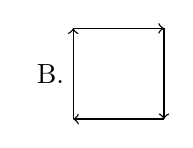
\begin{tikzpicture}[scale=0.72,line width=0.5pt]
\draw[->] (0,0)--(0,1.6);
\draw[->] (0,1.6)--(1.6,1.6);
\draw[->] (1.6,1.6)--(1.6,0);
\draw[->] (1.6,0)--(0,0);
\node at (-0.4,0.8) {B.};
\end{tikzpicture}
&
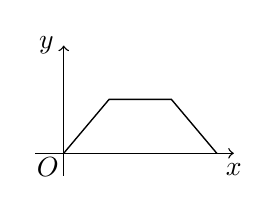
\begin{tikzpicture}[scale=0.72,line width=0.5pt]
\draw[->] (-0.5,0)--(3,0) node[below]{$x$};
\draw[->] (0,-0.4)--(0,1.9) node[left]{$y$};
\draw (0,0)--(0.8,0.95)--(1.9,0.95)--(2.7,0);
\node at (-0.28,-0.25) {$O$};
\end{tikzpicture}
\\
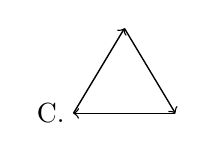
\begin{tikzpicture}[scale=0.72,line width=0.5pt]
\draw[->] (0,0)--(0.9,1.5);
\draw[->] (0.9,1.5)--(1.8,0);
\draw[->] (1.8,0)--(0,0);
\node at (-0.4,0) {C.};
\end{tikzpicture}
&
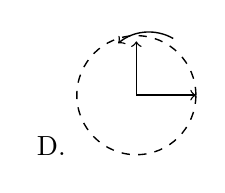
\begin{tikzpicture}[scale=0.72,line width=0.5pt]
\draw[dashed] (1.1,0.9) circle (1.05);
\draw[->] (1.1,0.9)--(2.15,0.9);
\draw[->] (1.1,0.9)--(1.1,1.85);
\draw[->] (1.75,1.9) arc (60:130:0.85);
\node at (-0.4,0) {D.};
\end{tikzpicture}
&
\end{tabular}
\end{center}

\ifanswer
\solbegin
\step{开始离家越来越远，中间离家距离不变，后来离家距离越来越近,}
\step{因此路线 $D$ 符合题意，故选 $D$.}
\solend
\fi

\item 若关于 $x$ 的方程 $ax^2+bx+c=0$（$a>0$）的两个实数根 $x_1$，$x_2$，集合
$S=\{x\mid x>x_1\}$，$T=\{x\mid x>x_2\}$，$P=\{x\mid x<x_1\}$，$Q=\{x\mid x<x_2\}$，则关于 $x$ 的不等式
$ax^2+bx+c>0$ 的解集为\mbox{（\quad）}

\keepwithprev
A. $(S\cap T)\cup(P\cap Q)$\qquad\qquad B. $(S\cap T)\cap(P\cap Q)$

C. $(S\cup T)\cup(P\cup Q)$\qquad\qquad D. $(S\cup T)\cap(P\cup Q)$

\ifanswer
\solbegin
\step{不妨设 $x_1<x_2$，则 $ax^2+bx+c>0$（$a>0$）的解集为 $\{x\mid x<x_1$ 或 $x>x_2\}$,}
\step{$S\cup T=\{x\mid x>x_1\}$，$P\cup Q=\{x\mid x<x_2\}$，$S\cap T=\{x\mid x>x_2\}$,}
\step{$P\cap Q=\{x\mid x<x_1\}$，所以 $(S\cap T)\cup(P\cap Q)=\{x\mid x<x_1$ 或 $x>x_2\}$. 故选 $A$.}
\solend
\fi

\item 已知存在函数 $y=f(x)$ 和 $y=g(x)$ 使得函数 $y=f(g(x))$ 的定义域为 $\R$，且表达式为
$f(g(x))=x^2$，则 $y=g(x)$ 的表达式不可能是\mbox{（\quad）}

\keepwithprev
A. $x^2-3\lvert x\rvert$\qquad B. $x^2+\sqrt{\lvert x\rvert}$\qquad C. $2x-1$\qquad D. $\lvert x\rvert$

\ifanswer
\solbegin
\step{对于选项 A，当 $g(x)=x^2-3\lvert x\rvert$ 时，$g(1)=g(2)=-2$.}
\step{由 $f(g(x))=x^2$ 得 $f(-2)=f(g(1))=1^2=1$，$f(-2)=f(g(2))=2^2=4$，% 原卷两处均作 f(-2)，照录
}
\step{与函数的定义矛盾，所以选项 A 不可能.}
\step{对于选项 B，当 $g(x)=x^2+\sqrt{\lvert x\rvert}$ 时,}
\step{令 $t=x^2+\sqrt{\lvert x\rvert}$，$s=\lvert x\rvert$，$h(s)=s^2+\sqrt s\ (s\geqslant0)$.}
\step{因为函数 $y=s^2$ 在区间 $[0,+\infty)$ 上严格增，函数 $y=\sqrt s$ 在区间 $[0,+\infty)$ 上严格增.}
\step{所以函数 $h(s)=s^2+\sqrt s\ (s\geqslant0)$ 在区间 $[0,+\infty)$ 上严格增.}
\step{故 $s=h^{-1}(t)$，即 $\lvert x\rvert=h^{-1}(t)$，因为 $f(g(x))=x^2=\lvert x\rvert^2$，所以 $f(t)=(h^{-1}(t))^2$,}
\step{即 $f(x)=(h^{-1}(x))^2$，此时 $y=f(g(x))$ 的定义域为 $\R$，故选项 B 可能.}
\step{对于选项 C，当 $g(x)=2x-1$ 时，由 $f(g(x))=x^2$ 得 $f(g(x))=f(2x-1)=x^2$,}
\step{则 $f(x)=\left(\dfrac{x+1}2\right)^2$，此时 $y=f(g(x))$ 的定义域为 $\R$，故选项 C 可能.}
\step{对于选项 D，当 $g(x)=\lvert x\rvert$ 时，由 $f(g(x))=x^2$ 得 $f(g(x))=f(\lvert x\rvert)=x^2$,}
\step{则 $f(x)=x^2\ (x\geqslant0)$，此时 $y=f(g(x))$ 的定义域为 $\R$，故选项 D 可能.}
\step{故选 $A$.}
\solend
\fi

\end{enumerate}

\bigsec{三、解答题}

\begin{enumerate}
\setcounter{enumi}{16}

\item 已知常数 $a\in\R$，集合 $A=\left\{x\,\middle|\,\dfrac{2x+11}{x+2}\geqslant3\right\}$，集合 $B=\{x\mid x^2+2ax-3a^2<0\}$.

（1）若 $a=2$，求 $A\cap B$；

（2）若 $A\cup B=A$，求实数 $a$ 的取值范围.

\ifanswer
\solbegin
\step{（1）$\dfrac{2x+11}{x+2}\geqslant3\Leftrightarrow\dfrac{-x+5}{x+2}\geqslant0\Leftrightarrow\dfrac{x-5}{x+2}\leqslant0\Leftrightarrow
\begin{cases}x+2\neq0\\(x-5)(x+2)\leqslant0\end{cases}$}
\step{$\Leftrightarrow-2<x\leqslant5$，$A=(-2,5]$,}
\step{当 $a=2$ 时，$B=\{x\mid x^2+4x-12<0\}=\{x\mid(x-2)(x+6)<0\}=(-6,2)$,}
\step{$A\cap B=(-2,2)$；}
\step{（2）由 $A\cup B=A$ 得 $B\subseteq A$,}
\step{当 $a=0$ 时，$B=\{x\mid x^2<0\}=\varnothing$，满足题意,}
\step{$x^2+2ax-3a^2=0$ 的两根分别是 $a$ 和 $-3a$,}
\step{当 $a>0$ 时，$B=(-3a,a)$，由题意得 $-2\leqslant-3a<a\leqslant5$，解得 $0<a\leqslant\dfrac23$,}
\step{当 $a<0$ 时，$B=(a,-3a)$，由题意得 $-2\leqslant a<-3a\leqslant5$，解得 $-\dfrac53\leqslant a<0$,}
\step{综上，$-\dfrac53\leqslant a\leqslant\dfrac23$.}
\solend
\fi

\item 某奶茶店今年年初花费 16 万元购买了一台制作冰淇淋的设备，经估算，该设备每年可
为该奶茶店提供 12 万元的总收入. 已知使用 $x$ 年（$x$ 为正整数）所需的各种维护费用总计为
$x^2+2x$ 万元（今年为第一年）.

（1）试问：该奶茶店第几年开始盈利（总收入超过总支出）？

（2）该奶茶店在若干年后要卖出该冰淇淋设备，有以下两种方案：

①当盈利总额达到最大值时，以 1 万元的价格卖出该设备；

②当年均盈利达到最大值时，以 2 万元的价格卖出该设备.

试问哪一种方案较为划算？请说明理由.

\ifanswer
\solbegin
\step{（1）由题意得总收入扣除支出后的纯收入 $y=12x-(x^2+2x+16)$}
\step{$=-x^2+10x-16$，$-x^2+10x-16>0$，解得 $2<x<8$,}
\step{由 $x\in\N^*$，所以从第三年开始盈利；}
\step{（2）方案①：纯收入 $y=-x^2+10x-16=-(x-5)^2+9$,}
\step{则 5 年后盈利总额达到最大值 9 万元，}
\step{以 1 万元的价格卖出该设备，共盈利 10 万元；}
\step{方案②：年均盈利 $z=\dfrac{-x^2+10x-16}{x}=-x+10-\dfrac{16}{x}$,}
\step{由 $x\in\N^*$，$x+\dfrac{16}{x}\geqslant2\sqrt{x\cdot\dfrac{16}{x}}=8$，当且仅当 $x=\dfrac{16}{x}$，即 $x=4$ 时取等号,}
\step{$z=-x+10-\dfrac{16}{x}\leqslant-8+10=2$，当 4 年后年均盈利达到最大值 2 万元时,}
\step{以 2 万元的价格卖出该设备，共盈利 $4\times2+2=10$ 万元.}
\step{两种方案盈利总数一样，但方案②时间短，较为划算.}
\solend
\fi

\item 已知常数 $m\in\R$，$f(x)=\sqrt{\sqrt{x(4-x)}-mx}$.% 原卷题干为双层根号，其解析按单层，见文件头注

（1）证明：对任意的 $m\in\R$，$\{x\mid y=f(x)\}\neq\varnothing$；

（2）若 $[0,2]\subseteq\{x\mid y=f(x)\}$，求实数 $m$ 的取值范围；

（3）若 $\{x\mid y=f(x)\}=[0,3]$，求实数 $m$ 的值.

\ifanswer
\solbegin
\step{（1）$\{x\mid y=f(x)\}=\{x\mid\sqrt{x(4-x)}-mx\geqslant0\}$,}
\step{由 $x(4-x)\geqslant0$ 得 $0\leqslant x\leqslant4$,}
\step{当 $m\leqslant0$ 时，由于 $0\leqslant x\leqslant4$,}
\step{所以 $\sqrt{x(4-x)}-mx\geqslant0$ 对任意 $0\leqslant x\leqslant4$ 恒成立,}
\step{故此时 $\{x\mid y=f(x)\}=\{x\mid0\leqslant x\leqslant4\}$，满足 $\{x\mid y=f(x)\}\neq\varnothing$,}
\step{当 $m>0$ 时，由于 $0\leqslant x\leqslant4$，所以 $mx\geqslant0$，所以 $x(4-x)\geqslant m^2x^2$,}
\step{得 $0\leqslant x\leqslant\dfrac4{1+m^2}$，故此时 $\{x\mid y=f(x)\}=\left\{x\,\middle|\,0\leqslant x\leqslant\dfrac4{1+m^2}\right\}$,}
\step{满足 $\{x\mid y=f(x)\}\neq\varnothing$,}
\step{所以，对任意的 $m\in\R$，$\{x\mid y=f(x)\}\neq\varnothing$；}
\step{（2）由（1）得当 $m\leqslant0$ 时，$\{x\mid y=f(x)\}=\{x\mid0\leqslant x\leqslant4\}$,}
\step{显然满足 $[0,2]\subseteq\{x\mid y=f(x)\}$.}
\step{当 $m>0$ 时，$\{x\mid y=f(x)\}=\left\{x\,\middle|\,0\leqslant x\leqslant\dfrac4{1+m^2}\right\}$,}
\step{由于 $[0,2]\subseteq\{x\mid y=f(x)\}$，所以 $\dfrac4{1+m^2}\geqslant2$，故 $0<m\leqslant1$,}
\step{综上，$m\leqslant1$；}
\step{（3）由于 $\{x\mid y=f(x)\}=[0,3]$,}
\step{所以 $m>0$，$\{x\mid y=f(x)\}=\left\{x\,\middle|\,0\leqslant x\leqslant\dfrac4{1+m^2}\right\}$,}
\step{因此 $\dfrac4{1+m^2}=3$，所以 $m=\dfrac{\sqrt3}3$.}
\solend
\fi

\item 已知函数 $y=f(x)$ 的定义域为 $\R$，其图像是一段连续曲线，对任意的 $a$、$b\in\R$，恒
有 $f(a-b)+f(a+b)=5f(a)\cdot f(b)$，且 $f(0)\neq0$，$f(1)=\dfrac23$.

（1）求 $f(0)$ 和 $f(2)$ 的值；

（2）判断函数 $y=f(x)$ 的奇偶性，并证明；

（3）证明：方程 $f(x)=5$ 在区间 $(2,3)$ 上有解.

\ifanswer
\solbegin
\step{（1）对任意的 $a$、$b\in\R$，恒有 $f(a-b)+f(a+b)=5f(a)\cdot f(b)$,}
\step{且 $f(0)\neq0$，$f(1)=\dfrac23$,}
\step{当 $a=1,b=0$ 时，$f(1)+f(1)=5f(1)\cdot f(0)$，解得 $f(0)=\dfrac25$,}
\step{当 $a=b=1$ 时，$f(0)+f(2)=5f(1)\cdot f(1)$，解得 $f(2)=\dfrac{82}{45}$；}
\step{（2）函数 $y=f(x)$ 为偶函数，证明如下：}
\step{当 $a=0,b=x$ 时，$f(-x)+f(x)=5f(0)\cdot f(x)=2f(x)$,}
\step{则有 $f(-x)=f(x)$，又函数 $y=f(x)$ 的定义域为 $\R$,}
\step{所以函数 $y=f(x)$ 为偶函数.}
\step{（2）$f(2)=\dfrac{82}{45}$% 原卷 (3) 的解答开头误标（2）并重印此行，照录
}
\step{当 $a=2,b=1$ 时，$f(1)+f(3)=5f(2)\cdot f(1)$，解得 $f(3)=\dfrac{146}{27}$,}
\step{函数 $y=f(x)$ 的图像是一段连续曲线，$\dfrac{82}{45}<5<\dfrac{146}{27}$,}
\step{所以存在 $x_0\in(2,3)$，使 $f(x_0)=5$,}
\step{即方程 $f(x)=5$ 在区间 $(2,3)$ 上有解.}
\solend
\fi

\item 若函数 $y=F(x)$ 的定义域为 $D$，且对于任意的 $x_1$、$x_2\in D$，“$F(x_1)=F(x_2)$”的充要
条件是“$x_1=x_2$”，则称函数 $y=F(x)$ 为 $D$ 上的“单值函数”. 对于函数 $y=f(x)$，记
$f^{(1)}(x)=f(x)$，$f^{(2)}(x)=f(f(x))$，$f^{(3)}(x)=f(f(f(x)))$，$\cdots$，$f^{(n+1)}(x)=f(f^{(n)}(x))$，其
中 $n=1,2,3,\cdots$，并对任意的 $A\subseteq D$，记集合 $f^{(n)}(A)=\left\{f^{(n)}(x)\mid x\in A\right\}$，并规定
$f^{(n)}(\varnothing)=\varnothing$.

（1）若 $f(x)=2x+1$，函数 $y=f(x)$ 的定义域为 $\R$，求 $f^{(2)}([0,1])$ 和 $f^{(3)}([0,1])$；

（2）若函数 $y=f(x)$ 的定义域为 $D$，且存在正整数 $m$，使得对任意的 $x\in D$，$f^{(m)}(x)=x$，
求证：函数 $y=f(x)$ 为 $D$ 上的“单值函数”；

（3）设 $a\in(0,1)$，若函数 $y=f(x)$ 的定义域为 $(0,1]$，且表达式为：
\[f(x)=\begin{cases}x+(1-a),&0<x\leqslant a,\\x-a,&a<x\leqslant1\end{cases}\]
判断 $y=f(x)$ 是否为 $(0,1]$ 上的“单值函数”，并证明对任
意的区间 $I\subseteq(0,1]$，存在正整数 $k$，使得 $f^{(k)}(I)\cap I\neq\varnothing$.

\ifanswer
\solbegin
\step{（1）当 $x\in[0,1]$ 时，$2x+1\in[1,3]$，所以 $f^{(1)}([0,1])=[1,3]$,}
\step{当 $x\in[1,3]$ 时，$2x+1\in[3,7]$，所以 $f^{(2)}([0,1])=[3,7]$,}
\step{当 $x\in[3,7]$ 时，$2x+1\in[7,15]$，所以 $f^{(3)}([0,1])=[7,15]$；}
\step{（2）由已知单值函数的定义可以改写为：若函数 $y=F(x)$ 的定义域为 $D$,}
\step{且对于任意的 $x_1$、$x_2\in D$，“$F(x_1)\neq F(x_2)$”的充要条件是“$x_1\neq x_2$”,}
\step{则称函数 $y=F(x)$ 为 $D$ 上的“单值函数.}
\step{假设 $f(x)$ 不是 $D$ 上的单值函数,}
\step{则存在 $x_1,x_2\in D,x_1\neq x_2$，$f(x_1)=f(x_2)$ 成立，即 $f^{(1)}(x_1)=f^{(1)}(x_2)$,}
\step{于是 $f\left[f^{(1)}(x_1)\right]=f\left[f^{(1)}(x_2)\right]$，即 $f^{(2)}(x_1)=f^{(2)}(x_2)$,}
\step{依此类推，得 $f^{(m)}(x_1)=f^{(m)}(x_2)$,}
\step{但由题意得 $f^{(m)}(x)=x$，因此 $f^{(2)}(x_1)=x_2$，$f^{(2)}(x_2)=x_2$，而 $x_1\neq x_2$,}
\step{因此 $f^{(m)}(x_1)\neq f^{(m)}(x_2)$，这样得出了矛盾的结论，所以假设不成立,}
\step{即 $f(x)$ 是 $D$ 上的单值函数；}
\step{（3）由新定义得 $f(x)=x+(1-a)$ 是单值函数，$f(x)=x-a$ 也是单值函数,}
\step{$0<a<1$，则 $0<1-a<1$,}
\step{又 $0<x\leqslant a$ 时，$f(x)=x+(1-a)\in(1-a,1]$,}
\step{$a<x\leqslant1$ 时，$f(x)=x-a\in(0,1-a]$，又 $(0,1-a]\cap(1-a,1]=\varnothing$,}
\step{因此对任意的 $x_1,x_2\in(0,1],x_1\neq x_2\Leftrightarrow f(x_1)\neq f(x_2)$,}
\step{所以 $y=f(x)$ 是 $(0,1]$ 上的“单值函数”,}
\step{对于任意的有限的区间 $I$，记 $\lvert I\rvert$ 表示区间 $I$ 的长度,}
\step{如果一个集合 $A$ 是若干个区间的并集,}
\step{则 $\lvert A\rvert$ 等于组成它的所有区间的长度之和,}
\step{对于任意的区间 $I\subseteq(0,1]$，$x\in I$，$f(I)=\{f(x)\mid x\in T\}$,}
\step{不妨设 $I=(s,t)$，$(0<s<t\leqslant1)$，$\lvert T\rvert=t-s$,}
\step{若 $(s,t)\subseteq(0,a]$，则 $f(I)=(s+1-a,t+1-a)$，$\lvert f(T)\rvert=t-s$,}
\step{若 $(s,t)\subseteq(a,1]$，则 $f(I)=(s-a,t-a)$，$\lvert f(T)\rvert=t-s$,}
\step{若 $a\in(s,t)$，则 $f(I)=(s+1-a,1]\cup(0,t-a)$,}
\step{$\lvert f(T)\rvert=1-(s+1-a)+(t-a)-0=t-s$，所以 $\lvert f(I)\rvert=\lvert I\rvert$,}
\step{对于任意的区间 $I\subseteq(0,1]$，显然存在正整数 $n$，使得 $n\lvert I\rvert>1$,}
\step{因此在 $f^{(0)}(I),f^{(1)}(I),f^{(2)}(I),\cdots,f^{(n)}(I)$（它们的长度和大于 1）中,}
\step{必然存在正整数 $m,l\ (m>l)$，使得 $f^{(m)}(I)\cap f^{(l)}(I)\neq\varnothing$,}
\step{因此必存在 $x,y\in I$，使得 $f^{(m)}(x)=f^{(l)}(y)$,}
\step{又 $y=f(x)$ 是 $(0,1]$ 上的单值函数,}
\step{所以 $f^{(m-1)}(x)=f^{(l-1)}(y)$，$f^{(m-2)}(x)=f^{(l-2)}(y)$，$\cdots$，$f^{(m-l)}(x)=y$,}
\step{这表示 $f^{(m-l)}(I)\cap I\neq\varnothing$，取 $k=m-l$,}
\step{所以对任意的区间 $I\subseteq(0,1]$，存在正整数 $k$，使得 $f^{(k)}(I)\cap I\neq\varnothing$.}
\solend
\fi

\end{enumerate}

\end{document}
"
% 紧凑版：xelatex "\def\iscompact{1}% 高一106_复旦附中_周末作业11期中复习.tex
%   —— 高一上数学“2026-2027 年复旦附中高一上周末作业 11 期中复习”（试卷版/答案版）
% 试卷版：xelatex 高一106_复旦附中_周末作业11期中复习.tex
% 答案版：xelatex "\def\isanswer{1}% 高一106_复旦附中_周末作业11期中复习.tex
%   —— 高一上数学“2026-2027 年复旦附中高一上周末作业 11 期中复习”（试卷版/答案版）
% 试卷版：xelatex 高一106_复旦附中_周末作业11期中复习.tex
% 答案版：xelatex "\def\isanswer{1}\input{高一106_复旦附中_周末作业11期中复习.tex}"
% 紧凑版：xelatex "\def\iscompact{1}\input{高一106_复旦附中_周末作业11期中复习.tex}"
%
% 原始材料：微信公众号“魔都数学加油站”文章，作者破晓，2026-11-03 17:19 发布；
% 连载“27学年高一106”，原文标题“27学年高一106——2026-2027年上海市复旦附中高一上周末作业11期中复习”；
% 原文链接：https://mp.weixin.qq.com/s/O3N1S8hA2awUzsOnRvCI-w。
% 正文为 9 张 PNG 页（第 1—2、4—8 页 4762×6735，第 3、9 页 2560×3620），题目下印有【解析】，为讲评版。
% 题目、解析均据原图转录；卷面水印及公众号页脚未录入。
% 第 14 题的四幅路线图选项与题干右侧的 $y$-$x$ 图像按原图形状用 TikZ 重绘。
%
% 卷首标题：原卷印作“2026-2027 年复旦附中高一上周末作业 11 期中复习”（公众号标题中的“上海市”
% 卷面标题行没有，本稿照卷面），年份区间按全稿惯例排 en dash；原卷未印副标题，本稿按题目内容
% 标为“集合与常用逻辑用语、不等式、函数”（期中复习跨三章）。
%
% 与原卷的排版差异：
%   ① 原文从第 3 题起，填空题编号为 3—12、选择题为 13—16、解答题为 17—21，本稿保留原题号；
%   ② 原卷每题下直接印【解析】，本稿按全稿惯例将解析置于答案版；第 13 题原卷把答案“$A$”
%      印在题干括号内且无【解析】，本稿试卷版留空、答案版提 \ans{}；
%   ③ 原卷未印副标题，本稿按“知识模块”口径补出；
%   ④ 原卷填空横线按全稿惯例排为 \blankline[4.4em]；解答题按惯例加 \ansspace；选择题括号排
%      \mbox{（\quad）}、选项段前按惯例加 \keepwithprev；
%   ⑤ 原卷数集排粗体 $\mathbf{R}$，按全稿惯例改 \R；
%   ⑥ 第 11 题题干“集　合　X”三字原卷字距拉得很开（铅字排版的空隙），本稿按正常字距排。
%
% 原卷存疑：第 16 题解析第二行原卷作“$f(-2)=f(g(1))=1^2=1$，$f(-2)=f(g(2))=2^2=4$”
% （两个都写 $f(-2)$；按 $g(1)=g(2)=-2$，两处相等正构成矛盾，但第二处按复合应写
% $f(g(2))=f(-2)$），本稿照录。第 19 题题干 $f(x)$ 为**双层根号**
% $\sqrt{\sqrt{x(4-x)}-mx}$，而解析 (1) 首行只写单层 $\sqrt{x(4-x)}-mx\geqslant0$
% （其后推导均按单层），原卷题干与解析不一致，各照录。
% 第 20 题解析 (3) 的解答开头原卷误标“（2）”并重印 $f(2)=\dfrac{82}{45}$ 一行，照录。
%
% 行数核对：逐题数 \step/\stepm 条数，合计 132 条（Q3：2；Q4：3；Q5：3；Q6：1；Q7：3；
% Q8：5；Q9：2；Q10：2；Q11：3；Q12：2；Q13：0；Q14：2；Q15：3；Q16：14；Q17：10；
% Q18：11；Q19：17；Q20：13；Q21：36），与原卷印刷行逐题相等。第 13 题括号内印答案、
% 无解析，提 \ans{}，不计入 \step 账。
%
\documentclass[a4paper,11pt]{article}
\usepackage{common}

\begin{document}

\examtitlest[3]{2026--2027 年复旦附中高一上周末作业 11 期中复习}{集合与常用逻辑用语、不等式、函数}

\bigsec{一、填空题}

\begin{enumerate}
\setcounter{enumi}{2}

\item 若关于 $x$ 的不等式组
$\begin{cases}2x+3>0\\x+3a<0\end{cases}$
的解集非空，则满足条件的最大整数 $a=$\blankline[4.4em].

\ifanswer
\solbegin
\step{由
$\begin{cases}2x+3>0\\x+3a<0\end{cases}$
得
$\begin{cases}x>-\dfrac32\\x<-3a\end{cases}$，
要使不等式组
$\begin{cases}2x+3>0\\x+3a<0\end{cases}$
的解集非空，}
\step{须 $-3a>-\dfrac32$，即 $a<\dfrac12$，故满足条件的最大整数 $a=0$.}
\solend
\fi

\item 若关于 $x$ 的不等式 $\lvert x-366\rvert+\lvert x-500\rvert\leqslant a$ 的解集非空，则 $a$ 的取值范围是\blankline[4.4em].

\ifanswer
\solbegin
\step{$\lvert x-366\rvert+\lvert x-500\rvert\geqslant\lvert x-366-(x-500)\rvert=134$,}
\step{当且仅当 $366\leqslant x\leqslant500$ 时取等号，所以 $\lvert x-366\rvert+\lvert x-500\rvert$ 的最小值为 134,}
\step{从而 $a\geqslant134$. 故 $a$ 的取值范围是 $[134,+\infty)$.}
\solend
\fi

\item 设集合 $A=\{1,2,3,4\}$，$B=\{1,2\}$，若 $C\subseteq A$ 且 $B\cap C\neq\varnothing$，则所有满足条件的集合 $C$ 的个数为\blankline[4.4em].

\ifanswer
\solbegin
\step{按题意，集合 $C$ 是 $A$ 的子集，且与 $B$ 的交集不为空集,}
\step{集合 $A$ 的子集有 $2^4=16$ 个，其中与 $B$ 的交集为空集的子集，即 $\{3,4\}$ 的子集,}
\step{有 $2^2=4$ 个，故满足题意的集合 $C$ 的个数为 $16-4=12$.}
\solend
\fi

\item 函数 $f(x)=\lvert x^2-3x+2\rvert$ 的单调增区间为\blankline[4.4em].

\ifanswer
\solbegin
\step{观察图像得函数 $f(x)=\lvert x^2-3x+2\rvert$ 的严格增区间为 $\left(1,\dfrac32\right),(2,+\infty)$.}
\solend
\fi

\item 已知 $f(x)=\sqrt{mx^2-mx+1}$，若函数 $y=f(x)$ 的定义域为 $\R$，则实数 $m$ 的取值范围为\blankline[4.4em].

\ifanswer
\solbegin
\step{当 $m=0$ 时，$f(x)=1$ 满足题意,}
\step{当 $m>0$ 时，$\Delta=m^2-4m\leqslant0$，所以 $0<m\leqslant4$,}
\step{故实数 $m$ 的取值范围为 $[0,4]$.}
\solend
\fi

\item 已知 $T$ 是方程 $x^2+px+q=0$（$p^2-4q>0$）的解集，$A=\{1,3,5,7,9\}$，$B=\{1,4,7,10\}$ 且 $T\cap A=\varnothing$，$T\cap B=T$，则 $p+q=$\blankline[4.4em].

\ifanswer
\solbegin
\step{对方程 $x^2+px+q=0$（$p^2-4q>0$），显然有两个根，故集合 $T$ 中有两个元素；}
\step{因为 $T\cap B=T$，所以 $T$ 中的两个元素一定在集合 $B$ 中；}
\step{又因为 $T\cap A=\varnothing$，故 $T$ 中的所有元素都不在 $A$ 中；}
\step{综上，$T$ 中的元素一定是 4 和 10，由根与系数的关系得 $14=-p,40=q$,}
\step{则 $p+q=26$.}
\solend
\fi

\item 已知正实数 $a$、$b$ 满足 $a+b=a^2+b^2$，则 $\dfrac1a+\dfrac1b$ 的最小值为\blankline[4.4em].

\ifanswer
\solbegin
\step{由已知 $\dfrac1a+\dfrac1b=\dfrac{a+b}{ab}=\dfrac{a^2+b^2}{ab}=\dfrac ab+\dfrac ba\geqslant2\sqrt{\dfrac ab\cdot\dfrac ba}=2$,}
\step{当且仅当 $\dfrac ba=\dfrac ab$，即 $a=b=1$ 时取等号，故 $\dfrac1a+\dfrac1b$ 的最小值为 $1$.}
\solend
\fi

\item 已知 $a$、$b$、$c$ 为实数，且 $a^2+c^2=64$，$b^2+c^2=100$，则 $a^2+b^2$ 的取值范围是\blankline[4.4em].

\ifanswer
\solbegin
\step{由题意得
$\begin{cases}a^2=64-c^2\\b^2=100-c^2\end{cases}\Rightarrow a^2+b^2=164-2c^2$，
其中 $0\leqslant c^2\leqslant64$,}
\step{因此 $a^2+b^2$ 的取值范围是 $[36,164]$.}
\solend
\fi

\item 设 $U$ 为全集，对集合 $X$，$Y$，定义运算“$*$”，$M*N=\overline{M\cap N}$. 已知全集
$U=\{1,2,3,4,5,6,7,8\}$，集合 $X=\{1,2,3\}$，$Y=\{3,4,5\}$，$Z=\{2,4,7\}$，则
$(X*Y)*Z=$\blankline[4.4em].% 原卷“集 合 X”三字字距拉得很开，本稿按正常字距排

\ifanswer
\solbegin
\step{因为集合 $U=\{1,2,3,4,5,6,7,8\}$，$X=\{1,2,3\}$，$Y=\{3,4,5\}$，$Z=\{2,4,7\}$,}
\step{所以 $X\cap Y=\{3\}$，则 $X*Y=\overline{X\cap Y}=\{1,2,4,5,6,7,8\}$,}
\step{又 $\{1,2,4,5,6,7,8\}\cap\{2,4,7\}=\{2,4,7\}$，所以 $(X*Y)*Z=\{1,3,5,6,8\}$.}
\solend
\fi

\item 已知一个奇函数 $y=f(x)$ 与一个偶函数 $y=g(x)$ 的和为函数 $y=\sqrt{x^2-3x+6}$，则 $f(3)=$\blankline[4.4em].

\ifanswer
\solbegin
\step{记 $h(x)=\sqrt{x^2-3x+6}$，由题意得
$\begin{cases}f(3)+g(3)=h(3)=\sqrt6\\f(-3)+g(-3)=h(-3)=2\sqrt6\end{cases}$,}
\step{又 $f(-3)=-f(3)$，$g(-3)=g(3)$，解得 $f(3)=-\dfrac{\sqrt6}2$.}
\solend
\fi

\end{enumerate}

\bigsec{二、选择题}

\begin{enumerate}
\setcounter{enumi}{12}

\item 已知 $a>b$ 均为正实数，则“$c>d$”是“$a+c>b+d$”的\mbox{（\quad）}条件% 原卷把答案“A”印在题干括号内、无【解析】

\keepwithprev
A. 充分非必要\qquad\qquad B. 必要不充分

C. 充分必要\qquad\qquad\qquad D. 既非充分又非必要

\ifanswer
\ans{$A$}
\fi

\item 如图是肖老师以恒定的速率夜跑时的离家距离 $(y)$ 与跑步时间 $(x)$ 之间的函数的图像，
则肖老师跑步的路线可能是\mbox{（\quad）}

\keepwithprev
\begin{center}
\begin{tabular}{ccc}
\begin{tikzpicture}[scale=0.72,line width=0.5pt]
\draw[->] (0,0)--(1.1,1.1);
\draw[->] (1.1,1.1)--(2.7,1.1);
\draw[->] (2.7,1.1)--(3.8,0);
\node at (-0.4,0) {A.};
\end{tikzpicture}
&
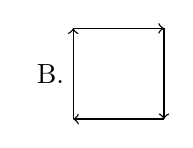
\begin{tikzpicture}[scale=0.72,line width=0.5pt]
\draw[->] (0,0)--(0,1.6);
\draw[->] (0,1.6)--(1.6,1.6);
\draw[->] (1.6,1.6)--(1.6,0);
\draw[->] (1.6,0)--(0,0);
\node at (-0.4,0.8) {B.};
\end{tikzpicture}
&
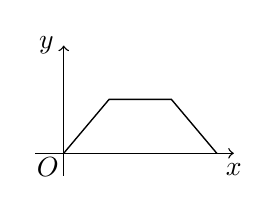
\begin{tikzpicture}[scale=0.72,line width=0.5pt]
\draw[->] (-0.5,0)--(3,0) node[below]{$x$};
\draw[->] (0,-0.4)--(0,1.9) node[left]{$y$};
\draw (0,0)--(0.8,0.95)--(1.9,0.95)--(2.7,0);
\node at (-0.28,-0.25) {$O$};
\end{tikzpicture}
\\
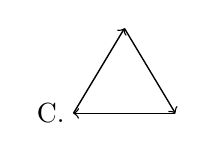
\begin{tikzpicture}[scale=0.72,line width=0.5pt]
\draw[->] (0,0)--(0.9,1.5);
\draw[->] (0.9,1.5)--(1.8,0);
\draw[->] (1.8,0)--(0,0);
\node at (-0.4,0) {C.};
\end{tikzpicture}
&
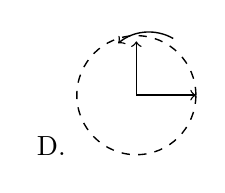
\begin{tikzpicture}[scale=0.72,line width=0.5pt]
\draw[dashed] (1.1,0.9) circle (1.05);
\draw[->] (1.1,0.9)--(2.15,0.9);
\draw[->] (1.1,0.9)--(1.1,1.85);
\draw[->] (1.75,1.9) arc (60:130:0.85);
\node at (-0.4,0) {D.};
\end{tikzpicture}
&
\end{tabular}
\end{center}

\ifanswer
\solbegin
\step{开始离家越来越远，中间离家距离不变，后来离家距离越来越近,}
\step{因此路线 $D$ 符合题意，故选 $D$.}
\solend
\fi

\item 若关于 $x$ 的方程 $ax^2+bx+c=0$（$a>0$）的两个实数根 $x_1$，$x_2$，集合
$S=\{x\mid x>x_1\}$，$T=\{x\mid x>x_2\}$，$P=\{x\mid x<x_1\}$，$Q=\{x\mid x<x_2\}$，则关于 $x$ 的不等式
$ax^2+bx+c>0$ 的解集为\mbox{（\quad）}

\keepwithprev
A. $(S\cap T)\cup(P\cap Q)$\qquad\qquad B. $(S\cap T)\cap(P\cap Q)$

C. $(S\cup T)\cup(P\cup Q)$\qquad\qquad D. $(S\cup T)\cap(P\cup Q)$

\ifanswer
\solbegin
\step{不妨设 $x_1<x_2$，则 $ax^2+bx+c>0$（$a>0$）的解集为 $\{x\mid x<x_1$ 或 $x>x_2\}$,}
\step{$S\cup T=\{x\mid x>x_1\}$，$P\cup Q=\{x\mid x<x_2\}$，$S\cap T=\{x\mid x>x_2\}$,}
\step{$P\cap Q=\{x\mid x<x_1\}$，所以 $(S\cap T)\cup(P\cap Q)=\{x\mid x<x_1$ 或 $x>x_2\}$. 故选 $A$.}
\solend
\fi

\item 已知存在函数 $y=f(x)$ 和 $y=g(x)$ 使得函数 $y=f(g(x))$ 的定义域为 $\R$，且表达式为
$f(g(x))=x^2$，则 $y=g(x)$ 的表达式不可能是\mbox{（\quad）}

\keepwithprev
A. $x^2-3\lvert x\rvert$\qquad B. $x^2+\sqrt{\lvert x\rvert}$\qquad C. $2x-1$\qquad D. $\lvert x\rvert$

\ifanswer
\solbegin
\step{对于选项 A，当 $g(x)=x^2-3\lvert x\rvert$ 时，$g(1)=g(2)=-2$.}
\step{由 $f(g(x))=x^2$ 得 $f(-2)=f(g(1))=1^2=1$，$f(-2)=f(g(2))=2^2=4$，% 原卷两处均作 f(-2)，照录
}
\step{与函数的定义矛盾，所以选项 A 不可能.}
\step{对于选项 B，当 $g(x)=x^2+\sqrt{\lvert x\rvert}$ 时,}
\step{令 $t=x^2+\sqrt{\lvert x\rvert}$，$s=\lvert x\rvert$，$h(s)=s^2+\sqrt s\ (s\geqslant0)$.}
\step{因为函数 $y=s^2$ 在区间 $[0,+\infty)$ 上严格增，函数 $y=\sqrt s$ 在区间 $[0,+\infty)$ 上严格增.}
\step{所以函数 $h(s)=s^2+\sqrt s\ (s\geqslant0)$ 在区间 $[0,+\infty)$ 上严格增.}
\step{故 $s=h^{-1}(t)$，即 $\lvert x\rvert=h^{-1}(t)$，因为 $f(g(x))=x^2=\lvert x\rvert^2$，所以 $f(t)=(h^{-1}(t))^2$,}
\step{即 $f(x)=(h^{-1}(x))^2$，此时 $y=f(g(x))$ 的定义域为 $\R$，故选项 B 可能.}
\step{对于选项 C，当 $g(x)=2x-1$ 时，由 $f(g(x))=x^2$ 得 $f(g(x))=f(2x-1)=x^2$,}
\step{则 $f(x)=\left(\dfrac{x+1}2\right)^2$，此时 $y=f(g(x))$ 的定义域为 $\R$，故选项 C 可能.}
\step{对于选项 D，当 $g(x)=\lvert x\rvert$ 时，由 $f(g(x))=x^2$ 得 $f(g(x))=f(\lvert x\rvert)=x^2$,}
\step{则 $f(x)=x^2\ (x\geqslant0)$，此时 $y=f(g(x))$ 的定义域为 $\R$，故选项 D 可能.}
\step{故选 $A$.}
\solend
\fi

\end{enumerate}

\bigsec{三、解答题}

\begin{enumerate}
\setcounter{enumi}{16}

\item 已知常数 $a\in\R$，集合 $A=\left\{x\,\middle|\,\dfrac{2x+11}{x+2}\geqslant3\right\}$，集合 $B=\{x\mid x^2+2ax-3a^2<0\}$.

（1）若 $a=2$，求 $A\cap B$；

（2）若 $A\cup B=A$，求实数 $a$ 的取值范围.

\ifanswer
\solbegin
\step{（1）$\dfrac{2x+11}{x+2}\geqslant3\Leftrightarrow\dfrac{-x+5}{x+2}\geqslant0\Leftrightarrow\dfrac{x-5}{x+2}\leqslant0\Leftrightarrow
\begin{cases}x+2\neq0\\(x-5)(x+2)\leqslant0\end{cases}$}
\step{$\Leftrightarrow-2<x\leqslant5$，$A=(-2,5]$,}
\step{当 $a=2$ 时，$B=\{x\mid x^2+4x-12<0\}=\{x\mid(x-2)(x+6)<0\}=(-6,2)$,}
\step{$A\cap B=(-2,2)$；}
\step{（2）由 $A\cup B=A$ 得 $B\subseteq A$,}
\step{当 $a=0$ 时，$B=\{x\mid x^2<0\}=\varnothing$，满足题意,}
\step{$x^2+2ax-3a^2=0$ 的两根分别是 $a$ 和 $-3a$,}
\step{当 $a>0$ 时，$B=(-3a,a)$，由题意得 $-2\leqslant-3a<a\leqslant5$，解得 $0<a\leqslant\dfrac23$,}
\step{当 $a<0$ 时，$B=(a,-3a)$，由题意得 $-2\leqslant a<-3a\leqslant5$，解得 $-\dfrac53\leqslant a<0$,}
\step{综上，$-\dfrac53\leqslant a\leqslant\dfrac23$.}
\solend
\fi

\item 某奶茶店今年年初花费 16 万元购买了一台制作冰淇淋的设备，经估算，该设备每年可
为该奶茶店提供 12 万元的总收入. 已知使用 $x$ 年（$x$ 为正整数）所需的各种维护费用总计为
$x^2+2x$ 万元（今年为第一年）.

（1）试问：该奶茶店第几年开始盈利（总收入超过总支出）？

（2）该奶茶店在若干年后要卖出该冰淇淋设备，有以下两种方案：

①当盈利总额达到最大值时，以 1 万元的价格卖出该设备；

②当年均盈利达到最大值时，以 2 万元的价格卖出该设备.

试问哪一种方案较为划算？请说明理由.

\ifanswer
\solbegin
\step{（1）由题意得总收入扣除支出后的纯收入 $y=12x-(x^2+2x+16)$}
\step{$=-x^2+10x-16$，$-x^2+10x-16>0$，解得 $2<x<8$,}
\step{由 $x\in\N^*$，所以从第三年开始盈利；}
\step{（2）方案①：纯收入 $y=-x^2+10x-16=-(x-5)^2+9$,}
\step{则 5 年后盈利总额达到最大值 9 万元，}
\step{以 1 万元的价格卖出该设备，共盈利 10 万元；}
\step{方案②：年均盈利 $z=\dfrac{-x^2+10x-16}{x}=-x+10-\dfrac{16}{x}$,}
\step{由 $x\in\N^*$，$x+\dfrac{16}{x}\geqslant2\sqrt{x\cdot\dfrac{16}{x}}=8$，当且仅当 $x=\dfrac{16}{x}$，即 $x=4$ 时取等号,}
\step{$z=-x+10-\dfrac{16}{x}\leqslant-8+10=2$，当 4 年后年均盈利达到最大值 2 万元时,}
\step{以 2 万元的价格卖出该设备，共盈利 $4\times2+2=10$ 万元.}
\step{两种方案盈利总数一样，但方案②时间短，较为划算.}
\solend
\fi

\item 已知常数 $m\in\R$，$f(x)=\sqrt{\sqrt{x(4-x)}-mx}$.% 原卷题干为双层根号，其解析按单层，见文件头注

（1）证明：对任意的 $m\in\R$，$\{x\mid y=f(x)\}\neq\varnothing$；

（2）若 $[0,2]\subseteq\{x\mid y=f(x)\}$，求实数 $m$ 的取值范围；

（3）若 $\{x\mid y=f(x)\}=[0,3]$，求实数 $m$ 的值.

\ifanswer
\solbegin
\step{（1）$\{x\mid y=f(x)\}=\{x\mid\sqrt{x(4-x)}-mx\geqslant0\}$,}
\step{由 $x(4-x)\geqslant0$ 得 $0\leqslant x\leqslant4$,}
\step{当 $m\leqslant0$ 时，由于 $0\leqslant x\leqslant4$,}
\step{所以 $\sqrt{x(4-x)}-mx\geqslant0$ 对任意 $0\leqslant x\leqslant4$ 恒成立,}
\step{故此时 $\{x\mid y=f(x)\}=\{x\mid0\leqslant x\leqslant4\}$，满足 $\{x\mid y=f(x)\}\neq\varnothing$,}
\step{当 $m>0$ 时，由于 $0\leqslant x\leqslant4$，所以 $mx\geqslant0$，所以 $x(4-x)\geqslant m^2x^2$,}
\step{得 $0\leqslant x\leqslant\dfrac4{1+m^2}$，故此时 $\{x\mid y=f(x)\}=\left\{x\,\middle|\,0\leqslant x\leqslant\dfrac4{1+m^2}\right\}$,}
\step{满足 $\{x\mid y=f(x)\}\neq\varnothing$,}
\step{所以，对任意的 $m\in\R$，$\{x\mid y=f(x)\}\neq\varnothing$；}
\step{（2）由（1）得当 $m\leqslant0$ 时，$\{x\mid y=f(x)\}=\{x\mid0\leqslant x\leqslant4\}$,}
\step{显然满足 $[0,2]\subseteq\{x\mid y=f(x)\}$.}
\step{当 $m>0$ 时，$\{x\mid y=f(x)\}=\left\{x\,\middle|\,0\leqslant x\leqslant\dfrac4{1+m^2}\right\}$,}
\step{由于 $[0,2]\subseteq\{x\mid y=f(x)\}$，所以 $\dfrac4{1+m^2}\geqslant2$，故 $0<m\leqslant1$,}
\step{综上，$m\leqslant1$；}
\step{（3）由于 $\{x\mid y=f(x)\}=[0,3]$,}
\step{所以 $m>0$，$\{x\mid y=f(x)\}=\left\{x\,\middle|\,0\leqslant x\leqslant\dfrac4{1+m^2}\right\}$,}
\step{因此 $\dfrac4{1+m^2}=3$，所以 $m=\dfrac{\sqrt3}3$.}
\solend
\fi

\item 已知函数 $y=f(x)$ 的定义域为 $\R$，其图像是一段连续曲线，对任意的 $a$、$b\in\R$，恒
有 $f(a-b)+f(a+b)=5f(a)\cdot f(b)$，且 $f(0)\neq0$，$f(1)=\dfrac23$.

（1）求 $f(0)$ 和 $f(2)$ 的值；

（2）判断函数 $y=f(x)$ 的奇偶性，并证明；

（3）证明：方程 $f(x)=5$ 在区间 $(2,3)$ 上有解.

\ifanswer
\solbegin
\step{（1）对任意的 $a$、$b\in\R$，恒有 $f(a-b)+f(a+b)=5f(a)\cdot f(b)$,}
\step{且 $f(0)\neq0$，$f(1)=\dfrac23$,}
\step{当 $a=1,b=0$ 时，$f(1)+f(1)=5f(1)\cdot f(0)$，解得 $f(0)=\dfrac25$,}
\step{当 $a=b=1$ 时，$f(0)+f(2)=5f(1)\cdot f(1)$，解得 $f(2)=\dfrac{82}{45}$；}
\step{（2）函数 $y=f(x)$ 为偶函数，证明如下：}
\step{当 $a=0,b=x$ 时，$f(-x)+f(x)=5f(0)\cdot f(x)=2f(x)$,}
\step{则有 $f(-x)=f(x)$，又函数 $y=f(x)$ 的定义域为 $\R$,}
\step{所以函数 $y=f(x)$ 为偶函数.}
\step{（2）$f(2)=\dfrac{82}{45}$% 原卷 (3) 的解答开头误标（2）并重印此行，照录
}
\step{当 $a=2,b=1$ 时，$f(1)+f(3)=5f(2)\cdot f(1)$，解得 $f(3)=\dfrac{146}{27}$,}
\step{函数 $y=f(x)$ 的图像是一段连续曲线，$\dfrac{82}{45}<5<\dfrac{146}{27}$,}
\step{所以存在 $x_0\in(2,3)$，使 $f(x_0)=5$,}
\step{即方程 $f(x)=5$ 在区间 $(2,3)$ 上有解.}
\solend
\fi

\item 若函数 $y=F(x)$ 的定义域为 $D$，且对于任意的 $x_1$、$x_2\in D$，“$F(x_1)=F(x_2)$”的充要
条件是“$x_1=x_2$”，则称函数 $y=F(x)$ 为 $D$ 上的“单值函数”. 对于函数 $y=f(x)$，记
$f^{(1)}(x)=f(x)$，$f^{(2)}(x)=f(f(x))$，$f^{(3)}(x)=f(f(f(x)))$，$\cdots$，$f^{(n+1)}(x)=f(f^{(n)}(x))$，其
中 $n=1,2,3,\cdots$，并对任意的 $A\subseteq D$，记集合 $f^{(n)}(A)=\left\{f^{(n)}(x)\mid x\in A\right\}$，并规定
$f^{(n)}(\varnothing)=\varnothing$.

（1）若 $f(x)=2x+1$，函数 $y=f(x)$ 的定义域为 $\R$，求 $f^{(2)}([0,1])$ 和 $f^{(3)}([0,1])$；

（2）若函数 $y=f(x)$ 的定义域为 $D$，且存在正整数 $m$，使得对任意的 $x\in D$，$f^{(m)}(x)=x$，
求证：函数 $y=f(x)$ 为 $D$ 上的“单值函数”；

（3）设 $a\in(0,1)$，若函数 $y=f(x)$ 的定义域为 $(0,1]$，且表达式为：
\[f(x)=\begin{cases}x+(1-a),&0<x\leqslant a,\\x-a,&a<x\leqslant1\end{cases}\]
判断 $y=f(x)$ 是否为 $(0,1]$ 上的“单值函数”，并证明对任
意的区间 $I\subseteq(0,1]$，存在正整数 $k$，使得 $f^{(k)}(I)\cap I\neq\varnothing$.

\ifanswer
\solbegin
\step{（1）当 $x\in[0,1]$ 时，$2x+1\in[1,3]$，所以 $f^{(1)}([0,1])=[1,3]$,}
\step{当 $x\in[1,3]$ 时，$2x+1\in[3,7]$，所以 $f^{(2)}([0,1])=[3,7]$,}
\step{当 $x\in[3,7]$ 时，$2x+1\in[7,15]$，所以 $f^{(3)}([0,1])=[7,15]$；}
\step{（2）由已知单值函数的定义可以改写为：若函数 $y=F(x)$ 的定义域为 $D$,}
\step{且对于任意的 $x_1$、$x_2\in D$，“$F(x_1)\neq F(x_2)$”的充要条件是“$x_1\neq x_2$”,}
\step{则称函数 $y=F(x)$ 为 $D$ 上的“单值函数.}
\step{假设 $f(x)$ 不是 $D$ 上的单值函数,}
\step{则存在 $x_1,x_2\in D,x_1\neq x_2$，$f(x_1)=f(x_2)$ 成立，即 $f^{(1)}(x_1)=f^{(1)}(x_2)$,}
\step{于是 $f\left[f^{(1)}(x_1)\right]=f\left[f^{(1)}(x_2)\right]$，即 $f^{(2)}(x_1)=f^{(2)}(x_2)$,}
\step{依此类推，得 $f^{(m)}(x_1)=f^{(m)}(x_2)$,}
\step{但由题意得 $f^{(m)}(x)=x$，因此 $f^{(2)}(x_1)=x_2$，$f^{(2)}(x_2)=x_2$，而 $x_1\neq x_2$,}
\step{因此 $f^{(m)}(x_1)\neq f^{(m)}(x_2)$，这样得出了矛盾的结论，所以假设不成立,}
\step{即 $f(x)$ 是 $D$ 上的单值函数；}
\step{（3）由新定义得 $f(x)=x+(1-a)$ 是单值函数，$f(x)=x-a$ 也是单值函数,}
\step{$0<a<1$，则 $0<1-a<1$,}
\step{又 $0<x\leqslant a$ 时，$f(x)=x+(1-a)\in(1-a,1]$,}
\step{$a<x\leqslant1$ 时，$f(x)=x-a\in(0,1-a]$，又 $(0,1-a]\cap(1-a,1]=\varnothing$,}
\step{因此对任意的 $x_1,x_2\in(0,1],x_1\neq x_2\Leftrightarrow f(x_1)\neq f(x_2)$,}
\step{所以 $y=f(x)$ 是 $(0,1]$ 上的“单值函数”,}
\step{对于任意的有限的区间 $I$，记 $\lvert I\rvert$ 表示区间 $I$ 的长度,}
\step{如果一个集合 $A$ 是若干个区间的并集,}
\step{则 $\lvert A\rvert$ 等于组成它的所有区间的长度之和,}
\step{对于任意的区间 $I\subseteq(0,1]$，$x\in I$，$f(I)=\{f(x)\mid x\in T\}$,}
\step{不妨设 $I=(s,t)$，$(0<s<t\leqslant1)$，$\lvert T\rvert=t-s$,}
\step{若 $(s,t)\subseteq(0,a]$，则 $f(I)=(s+1-a,t+1-a)$，$\lvert f(T)\rvert=t-s$,}
\step{若 $(s,t)\subseteq(a,1]$，则 $f(I)=(s-a,t-a)$，$\lvert f(T)\rvert=t-s$,}
\step{若 $a\in(s,t)$，则 $f(I)=(s+1-a,1]\cup(0,t-a)$,}
\step{$\lvert f(T)\rvert=1-(s+1-a)+(t-a)-0=t-s$，所以 $\lvert f(I)\rvert=\lvert I\rvert$,}
\step{对于任意的区间 $I\subseteq(0,1]$，显然存在正整数 $n$，使得 $n\lvert I\rvert>1$,}
\step{因此在 $f^{(0)}(I),f^{(1)}(I),f^{(2)}(I),\cdots,f^{(n)}(I)$（它们的长度和大于 1）中,}
\step{必然存在正整数 $m,l\ (m>l)$，使得 $f^{(m)}(I)\cap f^{(l)}(I)\neq\varnothing$,}
\step{因此必存在 $x,y\in I$，使得 $f^{(m)}(x)=f^{(l)}(y)$,}
\step{又 $y=f(x)$ 是 $(0,1]$ 上的单值函数,}
\step{所以 $f^{(m-1)}(x)=f^{(l-1)}(y)$，$f^{(m-2)}(x)=f^{(l-2)}(y)$，$\cdots$，$f^{(m-l)}(x)=y$,}
\step{这表示 $f^{(m-l)}(I)\cap I\neq\varnothing$，取 $k=m-l$,}
\step{所以对任意的区间 $I\subseteq(0,1]$，存在正整数 $k$，使得 $f^{(k)}(I)\cap I\neq\varnothing$.}
\solend
\fi

\end{enumerate}

\end{document}
"
% 紧凑版：xelatex "\def\iscompact{1}% 高一106_复旦附中_周末作业11期中复习.tex
%   —— 高一上数学“2026-2027 年复旦附中高一上周末作业 11 期中复习”（试卷版/答案版）
% 试卷版：xelatex 高一106_复旦附中_周末作业11期中复习.tex
% 答案版：xelatex "\def\isanswer{1}\input{高一106_复旦附中_周末作业11期中复习.tex}"
% 紧凑版：xelatex "\def\iscompact{1}\input{高一106_复旦附中_周末作业11期中复习.tex}"
%
% 原始材料：微信公众号“魔都数学加油站”文章，作者破晓，2026-11-03 17:19 发布；
% 连载“27学年高一106”，原文标题“27学年高一106——2026-2027年上海市复旦附中高一上周末作业11期中复习”；
% 原文链接：https://mp.weixin.qq.com/s/O3N1S8hA2awUzsOnRvCI-w。
% 正文为 9 张 PNG 页（第 1—2、4—8 页 4762×6735，第 3、9 页 2560×3620），题目下印有【解析】，为讲评版。
% 题目、解析均据原图转录；卷面水印及公众号页脚未录入。
% 第 14 题的四幅路线图选项与题干右侧的 $y$-$x$ 图像按原图形状用 TikZ 重绘。
%
% 卷首标题：原卷印作“2026-2027 年复旦附中高一上周末作业 11 期中复习”（公众号标题中的“上海市”
% 卷面标题行没有，本稿照卷面），年份区间按全稿惯例排 en dash；原卷未印副标题，本稿按题目内容
% 标为“集合与常用逻辑用语、不等式、函数”（期中复习跨三章）。
%
% 与原卷的排版差异：
%   ① 原文从第 3 题起，填空题编号为 3—12、选择题为 13—16、解答题为 17—21，本稿保留原题号；
%   ② 原卷每题下直接印【解析】，本稿按全稿惯例将解析置于答案版；第 13 题原卷把答案“$A$”
%      印在题干括号内且无【解析】，本稿试卷版留空、答案版提 \ans{}；
%   ③ 原卷未印副标题，本稿按“知识模块”口径补出；
%   ④ 原卷填空横线按全稿惯例排为 \blankline[4.4em]；解答题按惯例加 \ansspace；选择题括号排
%      \mbox{（\quad）}、选项段前按惯例加 \keepwithprev；
%   ⑤ 原卷数集排粗体 $\mathbf{R}$，按全稿惯例改 \R；
%   ⑥ 第 11 题题干“集　合　X”三字原卷字距拉得很开（铅字排版的空隙），本稿按正常字距排。
%
% 原卷存疑：第 16 题解析第二行原卷作“$f(-2)=f(g(1))=1^2=1$，$f(-2)=f(g(2))=2^2=4$”
% （两个都写 $f(-2)$；按 $g(1)=g(2)=-2$，两处相等正构成矛盾，但第二处按复合应写
% $f(g(2))=f(-2)$），本稿照录。第 19 题题干 $f(x)$ 为**双层根号**
% $\sqrt{\sqrt{x(4-x)}-mx}$，而解析 (1) 首行只写单层 $\sqrt{x(4-x)}-mx\geqslant0$
% （其后推导均按单层），原卷题干与解析不一致，各照录。
% 第 20 题解析 (3) 的解答开头原卷误标“（2）”并重印 $f(2)=\dfrac{82}{45}$ 一行，照录。
%
% 行数核对：逐题数 \step/\stepm 条数，合计 132 条（Q3：2；Q4：3；Q5：3；Q6：1；Q7：3；
% Q8：5；Q9：2；Q10：2；Q11：3；Q12：2；Q13：0；Q14：2；Q15：3；Q16：14；Q17：10；
% Q18：11；Q19：17；Q20：13；Q21：36），与原卷印刷行逐题相等。第 13 题括号内印答案、
% 无解析，提 \ans{}，不计入 \step 账。
%
\documentclass[a4paper,11pt]{article}
\usepackage{common}

\begin{document}

\examtitlest[3]{2026--2027 年复旦附中高一上周末作业 11 期中复习}{集合与常用逻辑用语、不等式、函数}

\bigsec{一、填空题}

\begin{enumerate}
\setcounter{enumi}{2}

\item 若关于 $x$ 的不等式组
$\begin{cases}2x+3>0\\x+3a<0\end{cases}$
的解集非空，则满足条件的最大整数 $a=$\blankline[4.4em].

\ifanswer
\solbegin
\step{由
$\begin{cases}2x+3>0\\x+3a<0\end{cases}$
得
$\begin{cases}x>-\dfrac32\\x<-3a\end{cases}$，
要使不等式组
$\begin{cases}2x+3>0\\x+3a<0\end{cases}$
的解集非空，}
\step{须 $-3a>-\dfrac32$，即 $a<\dfrac12$，故满足条件的最大整数 $a=0$.}
\solend
\fi

\item 若关于 $x$ 的不等式 $\lvert x-366\rvert+\lvert x-500\rvert\leqslant a$ 的解集非空，则 $a$ 的取值范围是\blankline[4.4em].

\ifanswer
\solbegin
\step{$\lvert x-366\rvert+\lvert x-500\rvert\geqslant\lvert x-366-(x-500)\rvert=134$,}
\step{当且仅当 $366\leqslant x\leqslant500$ 时取等号，所以 $\lvert x-366\rvert+\lvert x-500\rvert$ 的最小值为 134,}
\step{从而 $a\geqslant134$. 故 $a$ 的取值范围是 $[134,+\infty)$.}
\solend
\fi

\item 设集合 $A=\{1,2,3,4\}$，$B=\{1,2\}$，若 $C\subseteq A$ 且 $B\cap C\neq\varnothing$，则所有满足条件的集合 $C$ 的个数为\blankline[4.4em].

\ifanswer
\solbegin
\step{按题意，集合 $C$ 是 $A$ 的子集，且与 $B$ 的交集不为空集,}
\step{集合 $A$ 的子集有 $2^4=16$ 个，其中与 $B$ 的交集为空集的子集，即 $\{3,4\}$ 的子集,}
\step{有 $2^2=4$ 个，故满足题意的集合 $C$ 的个数为 $16-4=12$.}
\solend
\fi

\item 函数 $f(x)=\lvert x^2-3x+2\rvert$ 的单调增区间为\blankline[4.4em].

\ifanswer
\solbegin
\step{观察图像得函数 $f(x)=\lvert x^2-3x+2\rvert$ 的严格增区间为 $\left(1,\dfrac32\right),(2,+\infty)$.}
\solend
\fi

\item 已知 $f(x)=\sqrt{mx^2-mx+1}$，若函数 $y=f(x)$ 的定义域为 $\R$，则实数 $m$ 的取值范围为\blankline[4.4em].

\ifanswer
\solbegin
\step{当 $m=0$ 时，$f(x)=1$ 满足题意,}
\step{当 $m>0$ 时，$\Delta=m^2-4m\leqslant0$，所以 $0<m\leqslant4$,}
\step{故实数 $m$ 的取值范围为 $[0,4]$.}
\solend
\fi

\item 已知 $T$ 是方程 $x^2+px+q=0$（$p^2-4q>0$）的解集，$A=\{1,3,5,7,9\}$，$B=\{1,4,7,10\}$ 且 $T\cap A=\varnothing$，$T\cap B=T$，则 $p+q=$\blankline[4.4em].

\ifanswer
\solbegin
\step{对方程 $x^2+px+q=0$（$p^2-4q>0$），显然有两个根，故集合 $T$ 中有两个元素；}
\step{因为 $T\cap B=T$，所以 $T$ 中的两个元素一定在集合 $B$ 中；}
\step{又因为 $T\cap A=\varnothing$，故 $T$ 中的所有元素都不在 $A$ 中；}
\step{综上，$T$ 中的元素一定是 4 和 10，由根与系数的关系得 $14=-p,40=q$,}
\step{则 $p+q=26$.}
\solend
\fi

\item 已知正实数 $a$、$b$ 满足 $a+b=a^2+b^2$，则 $\dfrac1a+\dfrac1b$ 的最小值为\blankline[4.4em].

\ifanswer
\solbegin
\step{由已知 $\dfrac1a+\dfrac1b=\dfrac{a+b}{ab}=\dfrac{a^2+b^2}{ab}=\dfrac ab+\dfrac ba\geqslant2\sqrt{\dfrac ab\cdot\dfrac ba}=2$,}
\step{当且仅当 $\dfrac ba=\dfrac ab$，即 $a=b=1$ 时取等号，故 $\dfrac1a+\dfrac1b$ 的最小值为 $1$.}
\solend
\fi

\item 已知 $a$、$b$、$c$ 为实数，且 $a^2+c^2=64$，$b^2+c^2=100$，则 $a^2+b^2$ 的取值范围是\blankline[4.4em].

\ifanswer
\solbegin
\step{由题意得
$\begin{cases}a^2=64-c^2\\b^2=100-c^2\end{cases}\Rightarrow a^2+b^2=164-2c^2$，
其中 $0\leqslant c^2\leqslant64$,}
\step{因此 $a^2+b^2$ 的取值范围是 $[36,164]$.}
\solend
\fi

\item 设 $U$ 为全集，对集合 $X$，$Y$，定义运算“$*$”，$M*N=\overline{M\cap N}$. 已知全集
$U=\{1,2,3,4,5,6,7,8\}$，集合 $X=\{1,2,3\}$，$Y=\{3,4,5\}$，$Z=\{2,4,7\}$，则
$(X*Y)*Z=$\blankline[4.4em].% 原卷“集 合 X”三字字距拉得很开，本稿按正常字距排

\ifanswer
\solbegin
\step{因为集合 $U=\{1,2,3,4,5,6,7,8\}$，$X=\{1,2,3\}$，$Y=\{3,4,5\}$，$Z=\{2,4,7\}$,}
\step{所以 $X\cap Y=\{3\}$，则 $X*Y=\overline{X\cap Y}=\{1,2,4,5,6,7,8\}$,}
\step{又 $\{1,2,4,5,6,7,8\}\cap\{2,4,7\}=\{2,4,7\}$，所以 $(X*Y)*Z=\{1,3,5,6,8\}$.}
\solend
\fi

\item 已知一个奇函数 $y=f(x)$ 与一个偶函数 $y=g(x)$ 的和为函数 $y=\sqrt{x^2-3x+6}$，则 $f(3)=$\blankline[4.4em].

\ifanswer
\solbegin
\step{记 $h(x)=\sqrt{x^2-3x+6}$，由题意得
$\begin{cases}f(3)+g(3)=h(3)=\sqrt6\\f(-3)+g(-3)=h(-3)=2\sqrt6\end{cases}$,}
\step{又 $f(-3)=-f(3)$，$g(-3)=g(3)$，解得 $f(3)=-\dfrac{\sqrt6}2$.}
\solend
\fi

\end{enumerate}

\bigsec{二、选择题}

\begin{enumerate}
\setcounter{enumi}{12}

\item 已知 $a>b$ 均为正实数，则“$c>d$”是“$a+c>b+d$”的\mbox{（\quad）}条件% 原卷把答案“A”印在题干括号内、无【解析】

\keepwithprev
A. 充分非必要\qquad\qquad B. 必要不充分

C. 充分必要\qquad\qquad\qquad D. 既非充分又非必要

\ifanswer
\ans{$A$}
\fi

\item 如图是肖老师以恒定的速率夜跑时的离家距离 $(y)$ 与跑步时间 $(x)$ 之间的函数的图像，
则肖老师跑步的路线可能是\mbox{（\quad）}

\keepwithprev
\begin{center}
\begin{tabular}{ccc}
\begin{tikzpicture}[scale=0.72,line width=0.5pt]
\draw[->] (0,0)--(1.1,1.1);
\draw[->] (1.1,1.1)--(2.7,1.1);
\draw[->] (2.7,1.1)--(3.8,0);
\node at (-0.4,0) {A.};
\end{tikzpicture}
&
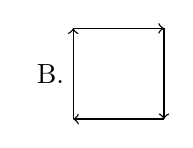
\begin{tikzpicture}[scale=0.72,line width=0.5pt]
\draw[->] (0,0)--(0,1.6);
\draw[->] (0,1.6)--(1.6,1.6);
\draw[->] (1.6,1.6)--(1.6,0);
\draw[->] (1.6,0)--(0,0);
\node at (-0.4,0.8) {B.};
\end{tikzpicture}
&
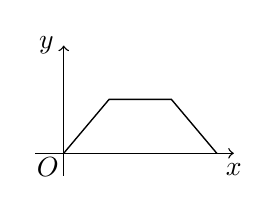
\begin{tikzpicture}[scale=0.72,line width=0.5pt]
\draw[->] (-0.5,0)--(3,0) node[below]{$x$};
\draw[->] (0,-0.4)--(0,1.9) node[left]{$y$};
\draw (0,0)--(0.8,0.95)--(1.9,0.95)--(2.7,0);
\node at (-0.28,-0.25) {$O$};
\end{tikzpicture}
\\
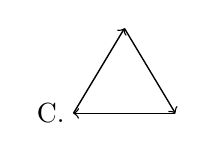
\begin{tikzpicture}[scale=0.72,line width=0.5pt]
\draw[->] (0,0)--(0.9,1.5);
\draw[->] (0.9,1.5)--(1.8,0);
\draw[->] (1.8,0)--(0,0);
\node at (-0.4,0) {C.};
\end{tikzpicture}
&
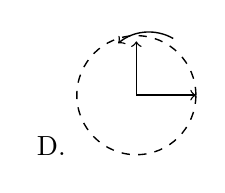
\begin{tikzpicture}[scale=0.72,line width=0.5pt]
\draw[dashed] (1.1,0.9) circle (1.05);
\draw[->] (1.1,0.9)--(2.15,0.9);
\draw[->] (1.1,0.9)--(1.1,1.85);
\draw[->] (1.75,1.9) arc (60:130:0.85);
\node at (-0.4,0) {D.};
\end{tikzpicture}
&
\end{tabular}
\end{center}

\ifanswer
\solbegin
\step{开始离家越来越远，中间离家距离不变，后来离家距离越来越近,}
\step{因此路线 $D$ 符合题意，故选 $D$.}
\solend
\fi

\item 若关于 $x$ 的方程 $ax^2+bx+c=0$（$a>0$）的两个实数根 $x_1$，$x_2$，集合
$S=\{x\mid x>x_1\}$，$T=\{x\mid x>x_2\}$，$P=\{x\mid x<x_1\}$，$Q=\{x\mid x<x_2\}$，则关于 $x$ 的不等式
$ax^2+bx+c>0$ 的解集为\mbox{（\quad）}

\keepwithprev
A. $(S\cap T)\cup(P\cap Q)$\qquad\qquad B. $(S\cap T)\cap(P\cap Q)$

C. $(S\cup T)\cup(P\cup Q)$\qquad\qquad D. $(S\cup T)\cap(P\cup Q)$

\ifanswer
\solbegin
\step{不妨设 $x_1<x_2$，则 $ax^2+bx+c>0$（$a>0$）的解集为 $\{x\mid x<x_1$ 或 $x>x_2\}$,}
\step{$S\cup T=\{x\mid x>x_1\}$，$P\cup Q=\{x\mid x<x_2\}$，$S\cap T=\{x\mid x>x_2\}$,}
\step{$P\cap Q=\{x\mid x<x_1\}$，所以 $(S\cap T)\cup(P\cap Q)=\{x\mid x<x_1$ 或 $x>x_2\}$. 故选 $A$.}
\solend
\fi

\item 已知存在函数 $y=f(x)$ 和 $y=g(x)$ 使得函数 $y=f(g(x))$ 的定义域为 $\R$，且表达式为
$f(g(x))=x^2$，则 $y=g(x)$ 的表达式不可能是\mbox{（\quad）}

\keepwithprev
A. $x^2-3\lvert x\rvert$\qquad B. $x^2+\sqrt{\lvert x\rvert}$\qquad C. $2x-1$\qquad D. $\lvert x\rvert$

\ifanswer
\solbegin
\step{对于选项 A，当 $g(x)=x^2-3\lvert x\rvert$ 时，$g(1)=g(2)=-2$.}
\step{由 $f(g(x))=x^2$ 得 $f(-2)=f(g(1))=1^2=1$，$f(-2)=f(g(2))=2^2=4$，% 原卷两处均作 f(-2)，照录
}
\step{与函数的定义矛盾，所以选项 A 不可能.}
\step{对于选项 B，当 $g(x)=x^2+\sqrt{\lvert x\rvert}$ 时,}
\step{令 $t=x^2+\sqrt{\lvert x\rvert}$，$s=\lvert x\rvert$，$h(s)=s^2+\sqrt s\ (s\geqslant0)$.}
\step{因为函数 $y=s^2$ 在区间 $[0,+\infty)$ 上严格增，函数 $y=\sqrt s$ 在区间 $[0,+\infty)$ 上严格增.}
\step{所以函数 $h(s)=s^2+\sqrt s\ (s\geqslant0)$ 在区间 $[0,+\infty)$ 上严格增.}
\step{故 $s=h^{-1}(t)$，即 $\lvert x\rvert=h^{-1}(t)$，因为 $f(g(x))=x^2=\lvert x\rvert^2$，所以 $f(t)=(h^{-1}(t))^2$,}
\step{即 $f(x)=(h^{-1}(x))^2$，此时 $y=f(g(x))$ 的定义域为 $\R$，故选项 B 可能.}
\step{对于选项 C，当 $g(x)=2x-1$ 时，由 $f(g(x))=x^2$ 得 $f(g(x))=f(2x-1)=x^2$,}
\step{则 $f(x)=\left(\dfrac{x+1}2\right)^2$，此时 $y=f(g(x))$ 的定义域为 $\R$，故选项 C 可能.}
\step{对于选项 D，当 $g(x)=\lvert x\rvert$ 时，由 $f(g(x))=x^2$ 得 $f(g(x))=f(\lvert x\rvert)=x^2$,}
\step{则 $f(x)=x^2\ (x\geqslant0)$，此时 $y=f(g(x))$ 的定义域为 $\R$，故选项 D 可能.}
\step{故选 $A$.}
\solend
\fi

\end{enumerate}

\bigsec{三、解答题}

\begin{enumerate}
\setcounter{enumi}{16}

\item 已知常数 $a\in\R$，集合 $A=\left\{x\,\middle|\,\dfrac{2x+11}{x+2}\geqslant3\right\}$，集合 $B=\{x\mid x^2+2ax-3a^2<0\}$.

（1）若 $a=2$，求 $A\cap B$；

（2）若 $A\cup B=A$，求实数 $a$ 的取值范围.

\ifanswer
\solbegin
\step{（1）$\dfrac{2x+11}{x+2}\geqslant3\Leftrightarrow\dfrac{-x+5}{x+2}\geqslant0\Leftrightarrow\dfrac{x-5}{x+2}\leqslant0\Leftrightarrow
\begin{cases}x+2\neq0\\(x-5)(x+2)\leqslant0\end{cases}$}
\step{$\Leftrightarrow-2<x\leqslant5$，$A=(-2,5]$,}
\step{当 $a=2$ 时，$B=\{x\mid x^2+4x-12<0\}=\{x\mid(x-2)(x+6)<0\}=(-6,2)$,}
\step{$A\cap B=(-2,2)$；}
\step{（2）由 $A\cup B=A$ 得 $B\subseteq A$,}
\step{当 $a=0$ 时，$B=\{x\mid x^2<0\}=\varnothing$，满足题意,}
\step{$x^2+2ax-3a^2=0$ 的两根分别是 $a$ 和 $-3a$,}
\step{当 $a>0$ 时，$B=(-3a,a)$，由题意得 $-2\leqslant-3a<a\leqslant5$，解得 $0<a\leqslant\dfrac23$,}
\step{当 $a<0$ 时，$B=(a,-3a)$，由题意得 $-2\leqslant a<-3a\leqslant5$，解得 $-\dfrac53\leqslant a<0$,}
\step{综上，$-\dfrac53\leqslant a\leqslant\dfrac23$.}
\solend
\fi

\item 某奶茶店今年年初花费 16 万元购买了一台制作冰淇淋的设备，经估算，该设备每年可
为该奶茶店提供 12 万元的总收入. 已知使用 $x$ 年（$x$ 为正整数）所需的各种维护费用总计为
$x^2+2x$ 万元（今年为第一年）.

（1）试问：该奶茶店第几年开始盈利（总收入超过总支出）？

（2）该奶茶店在若干年后要卖出该冰淇淋设备，有以下两种方案：

①当盈利总额达到最大值时，以 1 万元的价格卖出该设备；

②当年均盈利达到最大值时，以 2 万元的价格卖出该设备.

试问哪一种方案较为划算？请说明理由.

\ifanswer
\solbegin
\step{（1）由题意得总收入扣除支出后的纯收入 $y=12x-(x^2+2x+16)$}
\step{$=-x^2+10x-16$，$-x^2+10x-16>0$，解得 $2<x<8$,}
\step{由 $x\in\N^*$，所以从第三年开始盈利；}
\step{（2）方案①：纯收入 $y=-x^2+10x-16=-(x-5)^2+9$,}
\step{则 5 年后盈利总额达到最大值 9 万元，}
\step{以 1 万元的价格卖出该设备，共盈利 10 万元；}
\step{方案②：年均盈利 $z=\dfrac{-x^2+10x-16}{x}=-x+10-\dfrac{16}{x}$,}
\step{由 $x\in\N^*$，$x+\dfrac{16}{x}\geqslant2\sqrt{x\cdot\dfrac{16}{x}}=8$，当且仅当 $x=\dfrac{16}{x}$，即 $x=4$ 时取等号,}
\step{$z=-x+10-\dfrac{16}{x}\leqslant-8+10=2$，当 4 年后年均盈利达到最大值 2 万元时,}
\step{以 2 万元的价格卖出该设备，共盈利 $4\times2+2=10$ 万元.}
\step{两种方案盈利总数一样，但方案②时间短，较为划算.}
\solend
\fi

\item 已知常数 $m\in\R$，$f(x)=\sqrt{\sqrt{x(4-x)}-mx}$.% 原卷题干为双层根号，其解析按单层，见文件头注

（1）证明：对任意的 $m\in\R$，$\{x\mid y=f(x)\}\neq\varnothing$；

（2）若 $[0,2]\subseteq\{x\mid y=f(x)\}$，求实数 $m$ 的取值范围；

（3）若 $\{x\mid y=f(x)\}=[0,3]$，求实数 $m$ 的值.

\ifanswer
\solbegin
\step{（1）$\{x\mid y=f(x)\}=\{x\mid\sqrt{x(4-x)}-mx\geqslant0\}$,}
\step{由 $x(4-x)\geqslant0$ 得 $0\leqslant x\leqslant4$,}
\step{当 $m\leqslant0$ 时，由于 $0\leqslant x\leqslant4$,}
\step{所以 $\sqrt{x(4-x)}-mx\geqslant0$ 对任意 $0\leqslant x\leqslant4$ 恒成立,}
\step{故此时 $\{x\mid y=f(x)\}=\{x\mid0\leqslant x\leqslant4\}$，满足 $\{x\mid y=f(x)\}\neq\varnothing$,}
\step{当 $m>0$ 时，由于 $0\leqslant x\leqslant4$，所以 $mx\geqslant0$，所以 $x(4-x)\geqslant m^2x^2$,}
\step{得 $0\leqslant x\leqslant\dfrac4{1+m^2}$，故此时 $\{x\mid y=f(x)\}=\left\{x\,\middle|\,0\leqslant x\leqslant\dfrac4{1+m^2}\right\}$,}
\step{满足 $\{x\mid y=f(x)\}\neq\varnothing$,}
\step{所以，对任意的 $m\in\R$，$\{x\mid y=f(x)\}\neq\varnothing$；}
\step{（2）由（1）得当 $m\leqslant0$ 时，$\{x\mid y=f(x)\}=\{x\mid0\leqslant x\leqslant4\}$,}
\step{显然满足 $[0,2]\subseteq\{x\mid y=f(x)\}$.}
\step{当 $m>0$ 时，$\{x\mid y=f(x)\}=\left\{x\,\middle|\,0\leqslant x\leqslant\dfrac4{1+m^2}\right\}$,}
\step{由于 $[0,2]\subseteq\{x\mid y=f(x)\}$，所以 $\dfrac4{1+m^2}\geqslant2$，故 $0<m\leqslant1$,}
\step{综上，$m\leqslant1$；}
\step{（3）由于 $\{x\mid y=f(x)\}=[0,3]$,}
\step{所以 $m>0$，$\{x\mid y=f(x)\}=\left\{x\,\middle|\,0\leqslant x\leqslant\dfrac4{1+m^2}\right\}$,}
\step{因此 $\dfrac4{1+m^2}=3$，所以 $m=\dfrac{\sqrt3}3$.}
\solend
\fi

\item 已知函数 $y=f(x)$ 的定义域为 $\R$，其图像是一段连续曲线，对任意的 $a$、$b\in\R$，恒
有 $f(a-b)+f(a+b)=5f(a)\cdot f(b)$，且 $f(0)\neq0$，$f(1)=\dfrac23$.

（1）求 $f(0)$ 和 $f(2)$ 的值；

（2）判断函数 $y=f(x)$ 的奇偶性，并证明；

（3）证明：方程 $f(x)=5$ 在区间 $(2,3)$ 上有解.

\ifanswer
\solbegin
\step{（1）对任意的 $a$、$b\in\R$，恒有 $f(a-b)+f(a+b)=5f(a)\cdot f(b)$,}
\step{且 $f(0)\neq0$，$f(1)=\dfrac23$,}
\step{当 $a=1,b=0$ 时，$f(1)+f(1)=5f(1)\cdot f(0)$，解得 $f(0)=\dfrac25$,}
\step{当 $a=b=1$ 时，$f(0)+f(2)=5f(1)\cdot f(1)$，解得 $f(2)=\dfrac{82}{45}$；}
\step{（2）函数 $y=f(x)$ 为偶函数，证明如下：}
\step{当 $a=0,b=x$ 时，$f(-x)+f(x)=5f(0)\cdot f(x)=2f(x)$,}
\step{则有 $f(-x)=f(x)$，又函数 $y=f(x)$ 的定义域为 $\R$,}
\step{所以函数 $y=f(x)$ 为偶函数.}
\step{（2）$f(2)=\dfrac{82}{45}$% 原卷 (3) 的解答开头误标（2）并重印此行，照录
}
\step{当 $a=2,b=1$ 时，$f(1)+f(3)=5f(2)\cdot f(1)$，解得 $f(3)=\dfrac{146}{27}$,}
\step{函数 $y=f(x)$ 的图像是一段连续曲线，$\dfrac{82}{45}<5<\dfrac{146}{27}$,}
\step{所以存在 $x_0\in(2,3)$，使 $f(x_0)=5$,}
\step{即方程 $f(x)=5$ 在区间 $(2,3)$ 上有解.}
\solend
\fi

\item 若函数 $y=F(x)$ 的定义域为 $D$，且对于任意的 $x_1$、$x_2\in D$，“$F(x_1)=F(x_2)$”的充要
条件是“$x_1=x_2$”，则称函数 $y=F(x)$ 为 $D$ 上的“单值函数”. 对于函数 $y=f(x)$，记
$f^{(1)}(x)=f(x)$，$f^{(2)}(x)=f(f(x))$，$f^{(3)}(x)=f(f(f(x)))$，$\cdots$，$f^{(n+1)}(x)=f(f^{(n)}(x))$，其
中 $n=1,2,3,\cdots$，并对任意的 $A\subseteq D$，记集合 $f^{(n)}(A)=\left\{f^{(n)}(x)\mid x\in A\right\}$，并规定
$f^{(n)}(\varnothing)=\varnothing$.

（1）若 $f(x)=2x+1$，函数 $y=f(x)$ 的定义域为 $\R$，求 $f^{(2)}([0,1])$ 和 $f^{(3)}([0,1])$；

（2）若函数 $y=f(x)$ 的定义域为 $D$，且存在正整数 $m$，使得对任意的 $x\in D$，$f^{(m)}(x)=x$，
求证：函数 $y=f(x)$ 为 $D$ 上的“单值函数”；

（3）设 $a\in(0,1)$，若函数 $y=f(x)$ 的定义域为 $(0,1]$，且表达式为：
\[f(x)=\begin{cases}x+(1-a),&0<x\leqslant a,\\x-a,&a<x\leqslant1\end{cases}\]
判断 $y=f(x)$ 是否为 $(0,1]$ 上的“单值函数”，并证明对任
意的区间 $I\subseteq(0,1]$，存在正整数 $k$，使得 $f^{(k)}(I)\cap I\neq\varnothing$.

\ifanswer
\solbegin
\step{（1）当 $x\in[0,1]$ 时，$2x+1\in[1,3]$，所以 $f^{(1)}([0,1])=[1,3]$,}
\step{当 $x\in[1,3]$ 时，$2x+1\in[3,7]$，所以 $f^{(2)}([0,1])=[3,7]$,}
\step{当 $x\in[3,7]$ 时，$2x+1\in[7,15]$，所以 $f^{(3)}([0,1])=[7,15]$；}
\step{（2）由已知单值函数的定义可以改写为：若函数 $y=F(x)$ 的定义域为 $D$,}
\step{且对于任意的 $x_1$、$x_2\in D$，“$F(x_1)\neq F(x_2)$”的充要条件是“$x_1\neq x_2$”,}
\step{则称函数 $y=F(x)$ 为 $D$ 上的“单值函数.}
\step{假设 $f(x)$ 不是 $D$ 上的单值函数,}
\step{则存在 $x_1,x_2\in D,x_1\neq x_2$，$f(x_1)=f(x_2)$ 成立，即 $f^{(1)}(x_1)=f^{(1)}(x_2)$,}
\step{于是 $f\left[f^{(1)}(x_1)\right]=f\left[f^{(1)}(x_2)\right]$，即 $f^{(2)}(x_1)=f^{(2)}(x_2)$,}
\step{依此类推，得 $f^{(m)}(x_1)=f^{(m)}(x_2)$,}
\step{但由题意得 $f^{(m)}(x)=x$，因此 $f^{(2)}(x_1)=x_2$，$f^{(2)}(x_2)=x_2$，而 $x_1\neq x_2$,}
\step{因此 $f^{(m)}(x_1)\neq f^{(m)}(x_2)$，这样得出了矛盾的结论，所以假设不成立,}
\step{即 $f(x)$ 是 $D$ 上的单值函数；}
\step{（3）由新定义得 $f(x)=x+(1-a)$ 是单值函数，$f(x)=x-a$ 也是单值函数,}
\step{$0<a<1$，则 $0<1-a<1$,}
\step{又 $0<x\leqslant a$ 时，$f(x)=x+(1-a)\in(1-a,1]$,}
\step{$a<x\leqslant1$ 时，$f(x)=x-a\in(0,1-a]$，又 $(0,1-a]\cap(1-a,1]=\varnothing$,}
\step{因此对任意的 $x_1,x_2\in(0,1],x_1\neq x_2\Leftrightarrow f(x_1)\neq f(x_2)$,}
\step{所以 $y=f(x)$ 是 $(0,1]$ 上的“单值函数”,}
\step{对于任意的有限的区间 $I$，记 $\lvert I\rvert$ 表示区间 $I$ 的长度,}
\step{如果一个集合 $A$ 是若干个区间的并集,}
\step{则 $\lvert A\rvert$ 等于组成它的所有区间的长度之和,}
\step{对于任意的区间 $I\subseteq(0,1]$，$x\in I$，$f(I)=\{f(x)\mid x\in T\}$,}
\step{不妨设 $I=(s,t)$，$(0<s<t\leqslant1)$，$\lvert T\rvert=t-s$,}
\step{若 $(s,t)\subseteq(0,a]$，则 $f(I)=(s+1-a,t+1-a)$，$\lvert f(T)\rvert=t-s$,}
\step{若 $(s,t)\subseteq(a,1]$，则 $f(I)=(s-a,t-a)$，$\lvert f(T)\rvert=t-s$,}
\step{若 $a\in(s,t)$，则 $f(I)=(s+1-a,1]\cup(0,t-a)$,}
\step{$\lvert f(T)\rvert=1-(s+1-a)+(t-a)-0=t-s$，所以 $\lvert f(I)\rvert=\lvert I\rvert$,}
\step{对于任意的区间 $I\subseteq(0,1]$，显然存在正整数 $n$，使得 $n\lvert I\rvert>1$,}
\step{因此在 $f^{(0)}(I),f^{(1)}(I),f^{(2)}(I),\cdots,f^{(n)}(I)$（它们的长度和大于 1）中,}
\step{必然存在正整数 $m,l\ (m>l)$，使得 $f^{(m)}(I)\cap f^{(l)}(I)\neq\varnothing$,}
\step{因此必存在 $x,y\in I$，使得 $f^{(m)}(x)=f^{(l)}(y)$,}
\step{又 $y=f(x)$ 是 $(0,1]$ 上的单值函数,}
\step{所以 $f^{(m-1)}(x)=f^{(l-1)}(y)$，$f^{(m-2)}(x)=f^{(l-2)}(y)$，$\cdots$，$f^{(m-l)}(x)=y$,}
\step{这表示 $f^{(m-l)}(I)\cap I\neq\varnothing$，取 $k=m-l$,}
\step{所以对任意的区间 $I\subseteq(0,1]$，存在正整数 $k$，使得 $f^{(k)}(I)\cap I\neq\varnothing$.}
\solend
\fi

\end{enumerate}

\end{document}
"
%
% 原始材料：微信公众号“魔都数学加油站”文章，作者破晓，2026-11-03 17:19 发布；
% 连载“27学年高一106”，原文标题“27学年高一106——2026-2027年上海市复旦附中高一上周末作业11期中复习”；
% 原文链接：https://mp.weixin.qq.com/s/O3N1S8hA2awUzsOnRvCI-w。
% 正文为 9 张 PNG 页（第 1—2、4—8 页 4762×6735，第 3、9 页 2560×3620），题目下印有【解析】，为讲评版。
% 题目、解析均据原图转录；卷面水印及公众号页脚未录入。
% 第 14 题的四幅路线图选项与题干右侧的 $y$-$x$ 图像按原图形状用 TikZ 重绘。
%
% 卷首标题：原卷印作“2026-2027 年复旦附中高一上周末作业 11 期中复习”（公众号标题中的“上海市”
% 卷面标题行没有，本稿照卷面），年份区间按全稿惯例排 en dash；原卷未印副标题，本稿按题目内容
% 标为“集合与常用逻辑用语、不等式、函数”（期中复习跨三章）。
%
% 与原卷的排版差异：
%   ① 原文从第 3 题起，填空题编号为 3—12、选择题为 13—16、解答题为 17—21，本稿保留原题号；
%   ② 原卷每题下直接印【解析】，本稿按全稿惯例将解析置于答案版；第 13 题原卷把答案“$A$”
%      印在题干括号内且无【解析】，本稿试卷版留空、答案版提 \ans{}；
%   ③ 原卷未印副标题，本稿按“知识模块”口径补出；
%   ④ 原卷填空横线按全稿惯例排为 \blankline[4.4em]；解答题按惯例加 \ansspace；选择题括号排
%      \mbox{（\quad）}、选项段前按惯例加 \keepwithprev；
%   ⑤ 原卷数集排粗体 $\mathbf{R}$，按全稿惯例改 \R；
%   ⑥ 第 11 题题干“集　合　X”三字原卷字距拉得很开（铅字排版的空隙），本稿按正常字距排。
%
% 原卷存疑：第 16 题解析第二行原卷作“$f(-2)=f(g(1))=1^2=1$，$f(-2)=f(g(2))=2^2=4$”
% （两个都写 $f(-2)$；按 $g(1)=g(2)=-2$，两处相等正构成矛盾，但第二处按复合应写
% $f(g(2))=f(-2)$），本稿照录。第 19 题题干 $f(x)$ 为**双层根号**
% $\sqrt{\sqrt{x(4-x)}-mx}$，而解析 (1) 首行只写单层 $\sqrt{x(4-x)}-mx\geqslant0$
% （其后推导均按单层），原卷题干与解析不一致，各照录。
% 第 20 题解析 (3) 的解答开头原卷误标“（2）”并重印 $f(2)=\dfrac{82}{45}$ 一行，照录。
%
% 行数核对：逐题数 \step/\stepm 条数，合计 132 条（Q3：2；Q4：3；Q5：3；Q6：1；Q7：3；
% Q8：5；Q9：2；Q10：2；Q11：3；Q12：2；Q13：0；Q14：2；Q15：3；Q16：14；Q17：10；
% Q18：11；Q19：17；Q20：13；Q21：36），与原卷印刷行逐题相等。第 13 题括号内印答案、
% 无解析，提 \ans{}，不计入 \step 账。
%
\documentclass[a4paper,11pt]{article}
\usepackage{common}

\begin{document}

\examtitlest[3]{2026--2027 年复旦附中高一上周末作业 11 期中复习}{集合与常用逻辑用语、不等式、函数}

\bigsec{一、填空题}

\begin{enumerate}
\setcounter{enumi}{2}

\item 若关于 $x$ 的不等式组
$\begin{cases}2x+3>0\\x+3a<0\end{cases}$
的解集非空，则满足条件的最大整数 $a=$\blankline[4.4em].

\ifanswer
\solbegin
\step{由
$\begin{cases}2x+3>0\\x+3a<0\end{cases}$
得
$\begin{cases}x>-\dfrac32\\x<-3a\end{cases}$，
要使不等式组
$\begin{cases}2x+3>0\\x+3a<0\end{cases}$
的解集非空，}
\step{须 $-3a>-\dfrac32$，即 $a<\dfrac12$，故满足条件的最大整数 $a=0$.}
\solend
\fi

\item 若关于 $x$ 的不等式 $\lvert x-366\rvert+\lvert x-500\rvert\leqslant a$ 的解集非空，则 $a$ 的取值范围是\blankline[4.4em].

\ifanswer
\solbegin
\step{$\lvert x-366\rvert+\lvert x-500\rvert\geqslant\lvert x-366-(x-500)\rvert=134$,}
\step{当且仅当 $366\leqslant x\leqslant500$ 时取等号，所以 $\lvert x-366\rvert+\lvert x-500\rvert$ 的最小值为 134,}
\step{从而 $a\geqslant134$. 故 $a$ 的取值范围是 $[134,+\infty)$.}
\solend
\fi

\item 设集合 $A=\{1,2,3,4\}$，$B=\{1,2\}$，若 $C\subseteq A$ 且 $B\cap C\neq\varnothing$，则所有满足条件的集合 $C$ 的个数为\blankline[4.4em].

\ifanswer
\solbegin
\step{按题意，集合 $C$ 是 $A$ 的子集，且与 $B$ 的交集不为空集,}
\step{集合 $A$ 的子集有 $2^4=16$ 个，其中与 $B$ 的交集为空集的子集，即 $\{3,4\}$ 的子集,}
\step{有 $2^2=4$ 个，故满足题意的集合 $C$ 的个数为 $16-4=12$.}
\solend
\fi

\item 函数 $f(x)=\lvert x^2-3x+2\rvert$ 的单调增区间为\blankline[4.4em].

\ifanswer
\solbegin
\step{观察图像得函数 $f(x)=\lvert x^2-3x+2\rvert$ 的严格增区间为 $\left(1,\dfrac32\right),(2,+\infty)$.}
\solend
\fi

\item 已知 $f(x)=\sqrt{mx^2-mx+1}$，若函数 $y=f(x)$ 的定义域为 $\R$，则实数 $m$ 的取值范围为\blankline[4.4em].

\ifanswer
\solbegin
\step{当 $m=0$ 时，$f(x)=1$ 满足题意,}
\step{当 $m>0$ 时，$\Delta=m^2-4m\leqslant0$，所以 $0<m\leqslant4$,}
\step{故实数 $m$ 的取值范围为 $[0,4]$.}
\solend
\fi

\item 已知 $T$ 是方程 $x^2+px+q=0$（$p^2-4q>0$）的解集，$A=\{1,3,5,7,9\}$，$B=\{1,4,7,10\}$ 且 $T\cap A=\varnothing$，$T\cap B=T$，则 $p+q=$\blankline[4.4em].

\ifanswer
\solbegin
\step{对方程 $x^2+px+q=0$（$p^2-4q>0$），显然有两个根，故集合 $T$ 中有两个元素；}
\step{因为 $T\cap B=T$，所以 $T$ 中的两个元素一定在集合 $B$ 中；}
\step{又因为 $T\cap A=\varnothing$，故 $T$ 中的所有元素都不在 $A$ 中；}
\step{综上，$T$ 中的元素一定是 4 和 10，由根与系数的关系得 $14=-p,40=q$,}
\step{则 $p+q=26$.}
\solend
\fi

\item 已知正实数 $a$、$b$ 满足 $a+b=a^2+b^2$，则 $\dfrac1a+\dfrac1b$ 的最小值为\blankline[4.4em].

\ifanswer
\solbegin
\step{由已知 $\dfrac1a+\dfrac1b=\dfrac{a+b}{ab}=\dfrac{a^2+b^2}{ab}=\dfrac ab+\dfrac ba\geqslant2\sqrt{\dfrac ab\cdot\dfrac ba}=2$,}
\step{当且仅当 $\dfrac ba=\dfrac ab$，即 $a=b=1$ 时取等号，故 $\dfrac1a+\dfrac1b$ 的最小值为 $1$.}
\solend
\fi

\item 已知 $a$、$b$、$c$ 为实数，且 $a^2+c^2=64$，$b^2+c^2=100$，则 $a^2+b^2$ 的取值范围是\blankline[4.4em].

\ifanswer
\solbegin
\step{由题意得
$\begin{cases}a^2=64-c^2\\b^2=100-c^2\end{cases}\Rightarrow a^2+b^2=164-2c^2$，
其中 $0\leqslant c^2\leqslant64$,}
\step{因此 $a^2+b^2$ 的取值范围是 $[36,164]$.}
\solend
\fi

\item 设 $U$ 为全集，对集合 $X$，$Y$，定义运算“$*$”，$M*N=\overline{M\cap N}$. 已知全集
$U=\{1,2,3,4,5,6,7,8\}$，集合 $X=\{1,2,3\}$，$Y=\{3,4,5\}$，$Z=\{2,4,7\}$，则
$(X*Y)*Z=$\blankline[4.4em].% 原卷“集 合 X”三字字距拉得很开，本稿按正常字距排

\ifanswer
\solbegin
\step{因为集合 $U=\{1,2,3,4,5,6,7,8\}$，$X=\{1,2,3\}$，$Y=\{3,4,5\}$，$Z=\{2,4,7\}$,}
\step{所以 $X\cap Y=\{3\}$，则 $X*Y=\overline{X\cap Y}=\{1,2,4,5,6,7,8\}$,}
\step{又 $\{1,2,4,5,6,7,8\}\cap\{2,4,7\}=\{2,4,7\}$，所以 $(X*Y)*Z=\{1,3,5,6,8\}$.}
\solend
\fi

\item 已知一个奇函数 $y=f(x)$ 与一个偶函数 $y=g(x)$ 的和为函数 $y=\sqrt{x^2-3x+6}$，则 $f(3)=$\blankline[4.4em].

\ifanswer
\solbegin
\step{记 $h(x)=\sqrt{x^2-3x+6}$，由题意得
$\begin{cases}f(3)+g(3)=h(3)=\sqrt6\\f(-3)+g(-3)=h(-3)=2\sqrt6\end{cases}$,}
\step{又 $f(-3)=-f(3)$，$g(-3)=g(3)$，解得 $f(3)=-\dfrac{\sqrt6}2$.}
\solend
\fi

\end{enumerate}

\bigsec{二、选择题}

\begin{enumerate}
\setcounter{enumi}{12}

\item 已知 $a>b$ 均为正实数，则“$c>d$”是“$a+c>b+d$”的\mbox{（\quad）}条件% 原卷把答案“A”印在题干括号内、无【解析】

\keepwithprev
A. 充分非必要\qquad\qquad B. 必要不充分

C. 充分必要\qquad\qquad\qquad D. 既非充分又非必要

\ifanswer
\ans{$A$}
\fi

\item 如图是肖老师以恒定的速率夜跑时的离家距离 $(y)$ 与跑步时间 $(x)$ 之间的函数的图像，
则肖老师跑步的路线可能是\mbox{（\quad）}

\keepwithprev
\begin{center}
\begin{tabular}{ccc}
\begin{tikzpicture}[scale=0.72,line width=0.5pt]
\draw[->] (0,0)--(1.1,1.1);
\draw[->] (1.1,1.1)--(2.7,1.1);
\draw[->] (2.7,1.1)--(3.8,0);
\node at (-0.4,0) {A.};
\end{tikzpicture}
&
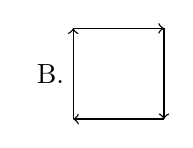
\begin{tikzpicture}[scale=0.72,line width=0.5pt]
\draw[->] (0,0)--(0,1.6);
\draw[->] (0,1.6)--(1.6,1.6);
\draw[->] (1.6,1.6)--(1.6,0);
\draw[->] (1.6,0)--(0,0);
\node at (-0.4,0.8) {B.};
\end{tikzpicture}
&
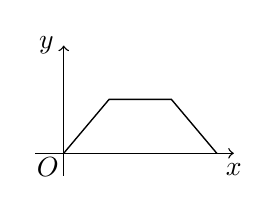
\begin{tikzpicture}[scale=0.72,line width=0.5pt]
\draw[->] (-0.5,0)--(3,0) node[below]{$x$};
\draw[->] (0,-0.4)--(0,1.9) node[left]{$y$};
\draw (0,0)--(0.8,0.95)--(1.9,0.95)--(2.7,0);
\node at (-0.28,-0.25) {$O$};
\end{tikzpicture}
\\
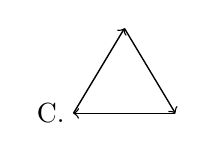
\begin{tikzpicture}[scale=0.72,line width=0.5pt]
\draw[->] (0,0)--(0.9,1.5);
\draw[->] (0.9,1.5)--(1.8,0);
\draw[->] (1.8,0)--(0,0);
\node at (-0.4,0) {C.};
\end{tikzpicture}
&
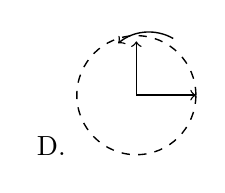
\begin{tikzpicture}[scale=0.72,line width=0.5pt]
\draw[dashed] (1.1,0.9) circle (1.05);
\draw[->] (1.1,0.9)--(2.15,0.9);
\draw[->] (1.1,0.9)--(1.1,1.85);
\draw[->] (1.75,1.9) arc (60:130:0.85);
\node at (-0.4,0) {D.};
\end{tikzpicture}
&
\end{tabular}
\end{center}

\ifanswer
\solbegin
\step{开始离家越来越远，中间离家距离不变，后来离家距离越来越近,}
\step{因此路线 $D$ 符合题意，故选 $D$.}
\solend
\fi

\item 若关于 $x$ 的方程 $ax^2+bx+c=0$（$a>0$）的两个实数根 $x_1$，$x_2$，集合
$S=\{x\mid x>x_1\}$，$T=\{x\mid x>x_2\}$，$P=\{x\mid x<x_1\}$，$Q=\{x\mid x<x_2\}$，则关于 $x$ 的不等式
$ax^2+bx+c>0$ 的解集为\mbox{（\quad）}

\keepwithprev
A. $(S\cap T)\cup(P\cap Q)$\qquad\qquad B. $(S\cap T)\cap(P\cap Q)$

C. $(S\cup T)\cup(P\cup Q)$\qquad\qquad D. $(S\cup T)\cap(P\cup Q)$

\ifanswer
\solbegin
\step{不妨设 $x_1<x_2$，则 $ax^2+bx+c>0$（$a>0$）的解集为 $\{x\mid x<x_1$ 或 $x>x_2\}$,}
\step{$S\cup T=\{x\mid x>x_1\}$，$P\cup Q=\{x\mid x<x_2\}$，$S\cap T=\{x\mid x>x_2\}$,}
\step{$P\cap Q=\{x\mid x<x_1\}$，所以 $(S\cap T)\cup(P\cap Q)=\{x\mid x<x_1$ 或 $x>x_2\}$. 故选 $A$.}
\solend
\fi

\item 已知存在函数 $y=f(x)$ 和 $y=g(x)$ 使得函数 $y=f(g(x))$ 的定义域为 $\R$，且表达式为
$f(g(x))=x^2$，则 $y=g(x)$ 的表达式不可能是\mbox{（\quad）}

\keepwithprev
A. $x^2-3\lvert x\rvert$\qquad B. $x^2+\sqrt{\lvert x\rvert}$\qquad C. $2x-1$\qquad D. $\lvert x\rvert$

\ifanswer
\solbegin
\step{对于选项 A，当 $g(x)=x^2-3\lvert x\rvert$ 时，$g(1)=g(2)=-2$.}
\step{由 $f(g(x))=x^2$ 得 $f(-2)=f(g(1))=1^2=1$，$f(-2)=f(g(2))=2^2=4$，% 原卷两处均作 f(-2)，照录
}
\step{与函数的定义矛盾，所以选项 A 不可能.}
\step{对于选项 B，当 $g(x)=x^2+\sqrt{\lvert x\rvert}$ 时,}
\step{令 $t=x^2+\sqrt{\lvert x\rvert}$，$s=\lvert x\rvert$，$h(s)=s^2+\sqrt s\ (s\geqslant0)$.}
\step{因为函数 $y=s^2$ 在区间 $[0,+\infty)$ 上严格增，函数 $y=\sqrt s$ 在区间 $[0,+\infty)$ 上严格增.}
\step{所以函数 $h(s)=s^2+\sqrt s\ (s\geqslant0)$ 在区间 $[0,+\infty)$ 上严格增.}
\step{故 $s=h^{-1}(t)$，即 $\lvert x\rvert=h^{-1}(t)$，因为 $f(g(x))=x^2=\lvert x\rvert^2$，所以 $f(t)=(h^{-1}(t))^2$,}
\step{即 $f(x)=(h^{-1}(x))^2$，此时 $y=f(g(x))$ 的定义域为 $\R$，故选项 B 可能.}
\step{对于选项 C，当 $g(x)=2x-1$ 时，由 $f(g(x))=x^2$ 得 $f(g(x))=f(2x-1)=x^2$,}
\step{则 $f(x)=\left(\dfrac{x+1}2\right)^2$，此时 $y=f(g(x))$ 的定义域为 $\R$，故选项 C 可能.}
\step{对于选项 D，当 $g(x)=\lvert x\rvert$ 时，由 $f(g(x))=x^2$ 得 $f(g(x))=f(\lvert x\rvert)=x^2$,}
\step{则 $f(x)=x^2\ (x\geqslant0)$，此时 $y=f(g(x))$ 的定义域为 $\R$，故选项 D 可能.}
\step{故选 $A$.}
\solend
\fi

\end{enumerate}

\bigsec{三、解答题}

\begin{enumerate}
\setcounter{enumi}{16}

\item 已知常数 $a\in\R$，集合 $A=\left\{x\,\middle|\,\dfrac{2x+11}{x+2}\geqslant3\right\}$，集合 $B=\{x\mid x^2+2ax-3a^2<0\}$.

（1）若 $a=2$，求 $A\cap B$；

（2）若 $A\cup B=A$，求实数 $a$ 的取值范围.

\ifanswer
\solbegin
\step{（1）$\dfrac{2x+11}{x+2}\geqslant3\Leftrightarrow\dfrac{-x+5}{x+2}\geqslant0\Leftrightarrow\dfrac{x-5}{x+2}\leqslant0\Leftrightarrow
\begin{cases}x+2\neq0\\(x-5)(x+2)\leqslant0\end{cases}$}
\step{$\Leftrightarrow-2<x\leqslant5$，$A=(-2,5]$,}
\step{当 $a=2$ 时，$B=\{x\mid x^2+4x-12<0\}=\{x\mid(x-2)(x+6)<0\}=(-6,2)$,}
\step{$A\cap B=(-2,2)$；}
\step{（2）由 $A\cup B=A$ 得 $B\subseteq A$,}
\step{当 $a=0$ 时，$B=\{x\mid x^2<0\}=\varnothing$，满足题意,}
\step{$x^2+2ax-3a^2=0$ 的两根分别是 $a$ 和 $-3a$,}
\step{当 $a>0$ 时，$B=(-3a,a)$，由题意得 $-2\leqslant-3a<a\leqslant5$，解得 $0<a\leqslant\dfrac23$,}
\step{当 $a<0$ 时，$B=(a,-3a)$，由题意得 $-2\leqslant a<-3a\leqslant5$，解得 $-\dfrac53\leqslant a<0$,}
\step{综上，$-\dfrac53\leqslant a\leqslant\dfrac23$.}
\solend
\fi

\item 某奶茶店今年年初花费 16 万元购买了一台制作冰淇淋的设备，经估算，该设备每年可
为该奶茶店提供 12 万元的总收入. 已知使用 $x$ 年（$x$ 为正整数）所需的各种维护费用总计为
$x^2+2x$ 万元（今年为第一年）.

（1）试问：该奶茶店第几年开始盈利（总收入超过总支出）？

（2）该奶茶店在若干年后要卖出该冰淇淋设备，有以下两种方案：

①当盈利总额达到最大值时，以 1 万元的价格卖出该设备；

②当年均盈利达到最大值时，以 2 万元的价格卖出该设备.

试问哪一种方案较为划算？请说明理由.

\ifanswer
\solbegin
\step{（1）由题意得总收入扣除支出后的纯收入 $y=12x-(x^2+2x+16)$}
\step{$=-x^2+10x-16$，$-x^2+10x-16>0$，解得 $2<x<8$,}
\step{由 $x\in\N^*$，所以从第三年开始盈利；}
\step{（2）方案①：纯收入 $y=-x^2+10x-16=-(x-5)^2+9$,}
\step{则 5 年后盈利总额达到最大值 9 万元，}
\step{以 1 万元的价格卖出该设备，共盈利 10 万元；}
\step{方案②：年均盈利 $z=\dfrac{-x^2+10x-16}{x}=-x+10-\dfrac{16}{x}$,}
\step{由 $x\in\N^*$，$x+\dfrac{16}{x}\geqslant2\sqrt{x\cdot\dfrac{16}{x}}=8$，当且仅当 $x=\dfrac{16}{x}$，即 $x=4$ 时取等号,}
\step{$z=-x+10-\dfrac{16}{x}\leqslant-8+10=2$，当 4 年后年均盈利达到最大值 2 万元时,}
\step{以 2 万元的价格卖出该设备，共盈利 $4\times2+2=10$ 万元.}
\step{两种方案盈利总数一样，但方案②时间短，较为划算.}
\solend
\fi

\item 已知常数 $m\in\R$，$f(x)=\sqrt{\sqrt{x(4-x)}-mx}$.% 原卷题干为双层根号，其解析按单层，见文件头注

（1）证明：对任意的 $m\in\R$，$\{x\mid y=f(x)\}\neq\varnothing$；

（2）若 $[0,2]\subseteq\{x\mid y=f(x)\}$，求实数 $m$ 的取值范围；

（3）若 $\{x\mid y=f(x)\}=[0,3]$，求实数 $m$ 的值.

\ifanswer
\solbegin
\step{（1）$\{x\mid y=f(x)\}=\{x\mid\sqrt{x(4-x)}-mx\geqslant0\}$,}
\step{由 $x(4-x)\geqslant0$ 得 $0\leqslant x\leqslant4$,}
\step{当 $m\leqslant0$ 时，由于 $0\leqslant x\leqslant4$,}
\step{所以 $\sqrt{x(4-x)}-mx\geqslant0$ 对任意 $0\leqslant x\leqslant4$ 恒成立,}
\step{故此时 $\{x\mid y=f(x)\}=\{x\mid0\leqslant x\leqslant4\}$，满足 $\{x\mid y=f(x)\}\neq\varnothing$,}
\step{当 $m>0$ 时，由于 $0\leqslant x\leqslant4$，所以 $mx\geqslant0$，所以 $x(4-x)\geqslant m^2x^2$,}
\step{得 $0\leqslant x\leqslant\dfrac4{1+m^2}$，故此时 $\{x\mid y=f(x)\}=\left\{x\,\middle|\,0\leqslant x\leqslant\dfrac4{1+m^2}\right\}$,}
\step{满足 $\{x\mid y=f(x)\}\neq\varnothing$,}
\step{所以，对任意的 $m\in\R$，$\{x\mid y=f(x)\}\neq\varnothing$；}
\step{（2）由（1）得当 $m\leqslant0$ 时，$\{x\mid y=f(x)\}=\{x\mid0\leqslant x\leqslant4\}$,}
\step{显然满足 $[0,2]\subseteq\{x\mid y=f(x)\}$.}
\step{当 $m>0$ 时，$\{x\mid y=f(x)\}=\left\{x\,\middle|\,0\leqslant x\leqslant\dfrac4{1+m^2}\right\}$,}
\step{由于 $[0,2]\subseteq\{x\mid y=f(x)\}$，所以 $\dfrac4{1+m^2}\geqslant2$，故 $0<m\leqslant1$,}
\step{综上，$m\leqslant1$；}
\step{（3）由于 $\{x\mid y=f(x)\}=[0,3]$,}
\step{所以 $m>0$，$\{x\mid y=f(x)\}=\left\{x\,\middle|\,0\leqslant x\leqslant\dfrac4{1+m^2}\right\}$,}
\step{因此 $\dfrac4{1+m^2}=3$，所以 $m=\dfrac{\sqrt3}3$.}
\solend
\fi

\item 已知函数 $y=f(x)$ 的定义域为 $\R$，其图像是一段连续曲线，对任意的 $a$、$b\in\R$，恒
有 $f(a-b)+f(a+b)=5f(a)\cdot f(b)$，且 $f(0)\neq0$，$f(1)=\dfrac23$.

（1）求 $f(0)$ 和 $f(2)$ 的值；

（2）判断函数 $y=f(x)$ 的奇偶性，并证明；

（3）证明：方程 $f(x)=5$ 在区间 $(2,3)$ 上有解.

\ifanswer
\solbegin
\step{（1）对任意的 $a$、$b\in\R$，恒有 $f(a-b)+f(a+b)=5f(a)\cdot f(b)$,}
\step{且 $f(0)\neq0$，$f(1)=\dfrac23$,}
\step{当 $a=1,b=0$ 时，$f(1)+f(1)=5f(1)\cdot f(0)$，解得 $f(0)=\dfrac25$,}
\step{当 $a=b=1$ 时，$f(0)+f(2)=5f(1)\cdot f(1)$，解得 $f(2)=\dfrac{82}{45}$；}
\step{（2）函数 $y=f(x)$ 为偶函数，证明如下：}
\step{当 $a=0,b=x$ 时，$f(-x)+f(x)=5f(0)\cdot f(x)=2f(x)$,}
\step{则有 $f(-x)=f(x)$，又函数 $y=f(x)$ 的定义域为 $\R$,}
\step{所以函数 $y=f(x)$ 为偶函数.}
\step{（2）$f(2)=\dfrac{82}{45}$% 原卷 (3) 的解答开头误标（2）并重印此行，照录
}
\step{当 $a=2,b=1$ 时，$f(1)+f(3)=5f(2)\cdot f(1)$，解得 $f(3)=\dfrac{146}{27}$,}
\step{函数 $y=f(x)$ 的图像是一段连续曲线，$\dfrac{82}{45}<5<\dfrac{146}{27}$,}
\step{所以存在 $x_0\in(2,3)$，使 $f(x_0)=5$,}
\step{即方程 $f(x)=5$ 在区间 $(2,3)$ 上有解.}
\solend
\fi

\item 若函数 $y=F(x)$ 的定义域为 $D$，且对于任意的 $x_1$、$x_2\in D$，“$F(x_1)=F(x_2)$”的充要
条件是“$x_1=x_2$”，则称函数 $y=F(x)$ 为 $D$ 上的“单值函数”. 对于函数 $y=f(x)$，记
$f^{(1)}(x)=f(x)$，$f^{(2)}(x)=f(f(x))$，$f^{(3)}(x)=f(f(f(x)))$，$\cdots$，$f^{(n+1)}(x)=f(f^{(n)}(x))$，其
中 $n=1,2,3,\cdots$，并对任意的 $A\subseteq D$，记集合 $f^{(n)}(A)=\left\{f^{(n)}(x)\mid x\in A\right\}$，并规定
$f^{(n)}(\varnothing)=\varnothing$.

（1）若 $f(x)=2x+1$，函数 $y=f(x)$ 的定义域为 $\R$，求 $f^{(2)}([0,1])$ 和 $f^{(3)}([0,1])$；

（2）若函数 $y=f(x)$ 的定义域为 $D$，且存在正整数 $m$，使得对任意的 $x\in D$，$f^{(m)}(x)=x$，
求证：函数 $y=f(x)$ 为 $D$ 上的“单值函数”；

（3）设 $a\in(0,1)$，若函数 $y=f(x)$ 的定义域为 $(0,1]$，且表达式为：
\[f(x)=\begin{cases}x+(1-a),&0<x\leqslant a,\\x-a,&a<x\leqslant1\end{cases}\]
判断 $y=f(x)$ 是否为 $(0,1]$ 上的“单值函数”，并证明对任
意的区间 $I\subseteq(0,1]$，存在正整数 $k$，使得 $f^{(k)}(I)\cap I\neq\varnothing$.

\ifanswer
\solbegin
\step{（1）当 $x\in[0,1]$ 时，$2x+1\in[1,3]$，所以 $f^{(1)}([0,1])=[1,3]$,}
\step{当 $x\in[1,3]$ 时，$2x+1\in[3,7]$，所以 $f^{(2)}([0,1])=[3,7]$,}
\step{当 $x\in[3,7]$ 时，$2x+1\in[7,15]$，所以 $f^{(3)}([0,1])=[7,15]$；}
\step{（2）由已知单值函数的定义可以改写为：若函数 $y=F(x)$ 的定义域为 $D$,}
\step{且对于任意的 $x_1$、$x_2\in D$，“$F(x_1)\neq F(x_2)$”的充要条件是“$x_1\neq x_2$”,}
\step{则称函数 $y=F(x)$ 为 $D$ 上的“单值函数.}
\step{假设 $f(x)$ 不是 $D$ 上的单值函数,}
\step{则存在 $x_1,x_2\in D,x_1\neq x_2$，$f(x_1)=f(x_2)$ 成立，即 $f^{(1)}(x_1)=f^{(1)}(x_2)$,}
\step{于是 $f\left[f^{(1)}(x_1)\right]=f\left[f^{(1)}(x_2)\right]$，即 $f^{(2)}(x_1)=f^{(2)}(x_2)$,}
\step{依此类推，得 $f^{(m)}(x_1)=f^{(m)}(x_2)$,}
\step{但由题意得 $f^{(m)}(x)=x$，因此 $f^{(2)}(x_1)=x_2$，$f^{(2)}(x_2)=x_2$，而 $x_1\neq x_2$,}
\step{因此 $f^{(m)}(x_1)\neq f^{(m)}(x_2)$，这样得出了矛盾的结论，所以假设不成立,}
\step{即 $f(x)$ 是 $D$ 上的单值函数；}
\step{（3）由新定义得 $f(x)=x+(1-a)$ 是单值函数，$f(x)=x-a$ 也是单值函数,}
\step{$0<a<1$，则 $0<1-a<1$,}
\step{又 $0<x\leqslant a$ 时，$f(x)=x+(1-a)\in(1-a,1]$,}
\step{$a<x\leqslant1$ 时，$f(x)=x-a\in(0,1-a]$，又 $(0,1-a]\cap(1-a,1]=\varnothing$,}
\step{因此对任意的 $x_1,x_2\in(0,1],x_1\neq x_2\Leftrightarrow f(x_1)\neq f(x_2)$,}
\step{所以 $y=f(x)$ 是 $(0,1]$ 上的“单值函数”,}
\step{对于任意的有限的区间 $I$，记 $\lvert I\rvert$ 表示区间 $I$ 的长度,}
\step{如果一个集合 $A$ 是若干个区间的并集,}
\step{则 $\lvert A\rvert$ 等于组成它的所有区间的长度之和,}
\step{对于任意的区间 $I\subseteq(0,1]$，$x\in I$，$f(I)=\{f(x)\mid x\in T\}$,}
\step{不妨设 $I=(s,t)$，$(0<s<t\leqslant1)$，$\lvert T\rvert=t-s$,}
\step{若 $(s,t)\subseteq(0,a]$，则 $f(I)=(s+1-a,t+1-a)$，$\lvert f(T)\rvert=t-s$,}
\step{若 $(s,t)\subseteq(a,1]$，则 $f(I)=(s-a,t-a)$，$\lvert f(T)\rvert=t-s$,}
\step{若 $a\in(s,t)$，则 $f(I)=(s+1-a,1]\cup(0,t-a)$,}
\step{$\lvert f(T)\rvert=1-(s+1-a)+(t-a)-0=t-s$，所以 $\lvert f(I)\rvert=\lvert I\rvert$,}
\step{对于任意的区间 $I\subseteq(0,1]$，显然存在正整数 $n$，使得 $n\lvert I\rvert>1$,}
\step{因此在 $f^{(0)}(I),f^{(1)}(I),f^{(2)}(I),\cdots,f^{(n)}(I)$（它们的长度和大于 1）中,}
\step{必然存在正整数 $m,l\ (m>l)$，使得 $f^{(m)}(I)\cap f^{(l)}(I)\neq\varnothing$,}
\step{因此必存在 $x,y\in I$，使得 $f^{(m)}(x)=f^{(l)}(y)$,}
\step{又 $y=f(x)$ 是 $(0,1]$ 上的单值函数,}
\step{所以 $f^{(m-1)}(x)=f^{(l-1)}(y)$，$f^{(m-2)}(x)=f^{(l-2)}(y)$，$\cdots$，$f^{(m-l)}(x)=y$,}
\step{这表示 $f^{(m-l)}(I)\cap I\neq\varnothing$，取 $k=m-l$,}
\step{所以对任意的区间 $I\subseteq(0,1]$，存在正整数 $k$，使得 $f^{(k)}(I)\cap I\neq\varnothing$.}
\solend
\fi

\end{enumerate}

\end{document}
"
%
% 原始材料：微信公众号“魔都数学加油站”文章，作者破晓，2026-11-03 17:19 发布；
% 连载“27学年高一106”，原文标题“27学年高一106——2026-2027年上海市复旦附中高一上周末作业11期中复习”；
% 原文链接：https://mp.weixin.qq.com/s/O3N1S8hA2awUzsOnRvCI-w。
% 正文为 9 张 PNG 页（第 1—2、4—8 页 4762×6735，第 3、9 页 2560×3620），题目下印有【解析】，为讲评版。
% 题目、解析均据原图转录；卷面水印及公众号页脚未录入。
% 第 14 题的四幅路线图选项与题干右侧的 $y$-$x$ 图像按原图形状用 TikZ 重绘。
%
% 卷首标题：原卷印作“2026-2027 年复旦附中高一上周末作业 11 期中复习”（公众号标题中的“上海市”
% 卷面标题行没有，本稿照卷面），年份区间按全稿惯例排 en dash；原卷未印副标题，本稿按题目内容
% 标为“集合与常用逻辑用语、不等式、函数”（期中复习跨三章）。
%
% 与原卷的排版差异：
%   ① 原文从第 3 题起，填空题编号为 3—12、选择题为 13—16、解答题为 17—21，本稿保留原题号；
%   ② 原卷每题下直接印【解析】，本稿按全稿惯例将解析置于答案版；第 13 题原卷把答案“$A$”
%      印在题干括号内且无【解析】，本稿试卷版留空、答案版提 \ans{}；
%   ③ 原卷未印副标题，本稿按“知识模块”口径补出；
%   ④ 原卷填空横线按全稿惯例排为 \blankline[4.4em]；解答题按惯例加 \ansspace；选择题括号排
%      \mbox{（\quad）}、选项段前按惯例加 \keepwithprev；
%   ⑤ 原卷数集排粗体 $\mathbf{R}$，按全稿惯例改 \R；
%   ⑥ 第 11 题题干“集　合　X”三字原卷字距拉得很开（铅字排版的空隙），本稿按正常字距排。
%
% 原卷存疑：第 16 题解析第二行原卷作“$f(-2)=f(g(1))=1^2=1$，$f(-2)=f(g(2))=2^2=4$”
% （两个都写 $f(-2)$；按 $g(1)=g(2)=-2$，两处相等正构成矛盾，但第二处按复合应写
% $f(g(2))=f(-2)$），本稿照录。第 19 题题干 $f(x)$ 为**双层根号**
% $\sqrt{\sqrt{x(4-x)}-mx}$，而解析 (1) 首行只写单层 $\sqrt{x(4-x)}-mx\geqslant0$
% （其后推导均按单层），原卷题干与解析不一致，各照录。
% 第 20 题解析 (3) 的解答开头原卷误标“（2）”并重印 $f(2)=\dfrac{82}{45}$ 一行，照录。
%
% 行数核对：逐题数 \step/\stepm 条数，合计 132 条（Q3：2；Q4：3；Q5：3；Q6：1；Q7：3；
% Q8：5；Q9：2；Q10：2；Q11：3；Q12：2；Q13：0；Q14：2；Q15：3；Q16：14；Q17：10；
% Q18：11；Q19：17；Q20：13；Q21：36），与原卷印刷行逐题相等。第 13 题括号内印答案、
% 无解析，提 \ans{}，不计入 \step 账。
%
\documentclass[a4paper,11pt]{article}
\usepackage{common}

\begin{document}

\examtitlest[3]{2026--2027 年复旦附中高一上周末作业 11 期中复习}{集合与常用逻辑用语、不等式、函数}

\bigsec{一、填空题}

\begin{enumerate}
\setcounter{enumi}{2}

\item 若关于 $x$ 的不等式组
$\begin{cases}2x+3>0\\x+3a<0\end{cases}$
的解集非空，则满足条件的最大整数 $a=$\blankline[4.4em].

\ifanswer
\solbegin
\step{由
$\begin{cases}2x+3>0\\x+3a<0\end{cases}$
得
$\begin{cases}x>-\dfrac32\\x<-3a\end{cases}$，
要使不等式组
$\begin{cases}2x+3>0\\x+3a<0\end{cases}$
的解集非空，}
\step{须 $-3a>-\dfrac32$，即 $a<\dfrac12$，故满足条件的最大整数 $a=0$.}
\solend
\fi

\item 若关于 $x$ 的不等式 $\lvert x-366\rvert+\lvert x-500\rvert\leqslant a$ 的解集非空，则 $a$ 的取值范围是\blankline[4.4em].

\ifanswer
\solbegin
\step{$\lvert x-366\rvert+\lvert x-500\rvert\geqslant\lvert x-366-(x-500)\rvert=134$,}
\step{当且仅当 $366\leqslant x\leqslant500$ 时取等号，所以 $\lvert x-366\rvert+\lvert x-500\rvert$ 的最小值为 134,}
\step{从而 $a\geqslant134$. 故 $a$ 的取值范围是 $[134,+\infty)$.}
\solend
\fi

\item 设集合 $A=\{1,2,3,4\}$，$B=\{1,2\}$，若 $C\subseteq A$ 且 $B\cap C\neq\varnothing$，则所有满足条件的集合 $C$ 的个数为\blankline[4.4em].

\ifanswer
\solbegin
\step{按题意，集合 $C$ 是 $A$ 的子集，且与 $B$ 的交集不为空集,}
\step{集合 $A$ 的子集有 $2^4=16$ 个，其中与 $B$ 的交集为空集的子集，即 $\{3,4\}$ 的子集,}
\step{有 $2^2=4$ 个，故满足题意的集合 $C$ 的个数为 $16-4=12$.}
\solend
\fi

\item 函数 $f(x)=\lvert x^2-3x+2\rvert$ 的单调增区间为\blankline[4.4em].

\ifanswer
\solbegin
\step{观察图像得函数 $f(x)=\lvert x^2-3x+2\rvert$ 的严格增区间为 $\left(1,\dfrac32\right),(2,+\infty)$.}
\solend
\fi

\item 已知 $f(x)=\sqrt{mx^2-mx+1}$，若函数 $y=f(x)$ 的定义域为 $\R$，则实数 $m$ 的取值范围为\blankline[4.4em].

\ifanswer
\solbegin
\step{当 $m=0$ 时，$f(x)=1$ 满足题意,}
\step{当 $m>0$ 时，$\Delta=m^2-4m\leqslant0$，所以 $0<m\leqslant4$,}
\step{故实数 $m$ 的取值范围为 $[0,4]$.}
\solend
\fi

\item 已知 $T$ 是方程 $x^2+px+q=0$（$p^2-4q>0$）的解集，$A=\{1,3,5,7,9\}$，$B=\{1,4,7,10\}$ 且 $T\cap A=\varnothing$，$T\cap B=T$，则 $p+q=$\blankline[4.4em].

\ifanswer
\solbegin
\step{对方程 $x^2+px+q=0$（$p^2-4q>0$），显然有两个根，故集合 $T$ 中有两个元素；}
\step{因为 $T\cap B=T$，所以 $T$ 中的两个元素一定在集合 $B$ 中；}
\step{又因为 $T\cap A=\varnothing$，故 $T$ 中的所有元素都不在 $A$ 中；}
\step{综上，$T$ 中的元素一定是 4 和 10，由根与系数的关系得 $14=-p,40=q$,}
\step{则 $p+q=26$.}
\solend
\fi

\item 已知正实数 $a$、$b$ 满足 $a+b=a^2+b^2$，则 $\dfrac1a+\dfrac1b$ 的最小值为\blankline[4.4em].

\ifanswer
\solbegin
\step{由已知 $\dfrac1a+\dfrac1b=\dfrac{a+b}{ab}=\dfrac{a^2+b^2}{ab}=\dfrac ab+\dfrac ba\geqslant2\sqrt{\dfrac ab\cdot\dfrac ba}=2$,}
\step{当且仅当 $\dfrac ba=\dfrac ab$，即 $a=b=1$ 时取等号，故 $\dfrac1a+\dfrac1b$ 的最小值为 $1$.}
\solend
\fi

\item 已知 $a$、$b$、$c$ 为实数，且 $a^2+c^2=64$，$b^2+c^2=100$，则 $a^2+b^2$ 的取值范围是\blankline[4.4em].

\ifanswer
\solbegin
\step{由题意得
$\begin{cases}a^2=64-c^2\\b^2=100-c^2\end{cases}\Rightarrow a^2+b^2=164-2c^2$，
其中 $0\leqslant c^2\leqslant64$,}
\step{因此 $a^2+b^2$ 的取值范围是 $[36,164]$.}
\solend
\fi

\item 设 $U$ 为全集，对集合 $X$，$Y$，定义运算“$*$”，$M*N=\overline{M\cap N}$. 已知全集
$U=\{1,2,3,4,5,6,7,8\}$，集合 $X=\{1,2,3\}$，$Y=\{3,4,5\}$，$Z=\{2,4,7\}$，则
$(X*Y)*Z=$\blankline[4.4em].% 原卷“集 合 X”三字字距拉得很开，本稿按正常字距排

\ifanswer
\solbegin
\step{因为集合 $U=\{1,2,3,4,5,6,7,8\}$，$X=\{1,2,3\}$，$Y=\{3,4,5\}$，$Z=\{2,4,7\}$,}
\step{所以 $X\cap Y=\{3\}$，则 $X*Y=\overline{X\cap Y}=\{1,2,4,5,6,7,8\}$,}
\step{又 $\{1,2,4,5,6,7,8\}\cap\{2,4,7\}=\{2,4,7\}$，所以 $(X*Y)*Z=\{1,3,5,6,8\}$.}
\solend
\fi

\item 已知一个奇函数 $y=f(x)$ 与一个偶函数 $y=g(x)$ 的和为函数 $y=\sqrt{x^2-3x+6}$，则 $f(3)=$\blankline[4.4em].

\ifanswer
\solbegin
\step{记 $h(x)=\sqrt{x^2-3x+6}$，由题意得
$\begin{cases}f(3)+g(3)=h(3)=\sqrt6\\f(-3)+g(-3)=h(-3)=2\sqrt6\end{cases}$,}
\step{又 $f(-3)=-f(3)$，$g(-3)=g(3)$，解得 $f(3)=-\dfrac{\sqrt6}2$.}
\solend
\fi

\end{enumerate}

\bigsec{二、选择题}

\begin{enumerate}
\setcounter{enumi}{12}

\item 已知 $a>b$ 均为正实数，则“$c>d$”是“$a+c>b+d$”的\mbox{（\quad）}条件% 原卷把答案“A”印在题干括号内、无【解析】

\keepwithprev
A. 充分非必要\qquad\qquad B. 必要不充分

C. 充分必要\qquad\qquad\qquad D. 既非充分又非必要

\ifanswer
\ans{$A$}
\fi

\item 如图是肖老师以恒定的速率夜跑时的离家距离 $(y)$ 与跑步时间 $(x)$ 之间的函数的图像，
则肖老师跑步的路线可能是\mbox{（\quad）}

\keepwithprev
\begin{center}
\begin{tabular}{ccc}
\begin{tikzpicture}[scale=0.72,line width=0.5pt]
\draw[->] (0,0)--(1.1,1.1);
\draw[->] (1.1,1.1)--(2.7,1.1);
\draw[->] (2.7,1.1)--(3.8,0);
\node at (-0.4,0) {A.};
\end{tikzpicture}
&
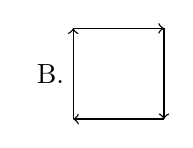
\begin{tikzpicture}[scale=0.72,line width=0.5pt]
\draw[->] (0,0)--(0,1.6);
\draw[->] (0,1.6)--(1.6,1.6);
\draw[->] (1.6,1.6)--(1.6,0);
\draw[->] (1.6,0)--(0,0);
\node at (-0.4,0.8) {B.};
\end{tikzpicture}
&
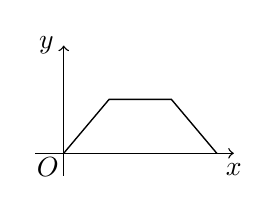
\begin{tikzpicture}[scale=0.72,line width=0.5pt]
\draw[->] (-0.5,0)--(3,0) node[below]{$x$};
\draw[->] (0,-0.4)--(0,1.9) node[left]{$y$};
\draw (0,0)--(0.8,0.95)--(1.9,0.95)--(2.7,0);
\node at (-0.28,-0.25) {$O$};
\end{tikzpicture}
\\
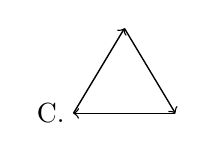
\begin{tikzpicture}[scale=0.72,line width=0.5pt]
\draw[->] (0,0)--(0.9,1.5);
\draw[->] (0.9,1.5)--(1.8,0);
\draw[->] (1.8,0)--(0,0);
\node at (-0.4,0) {C.};
\end{tikzpicture}
&
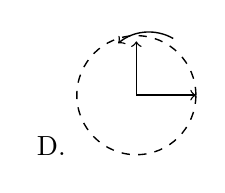
\begin{tikzpicture}[scale=0.72,line width=0.5pt]
\draw[dashed] (1.1,0.9) circle (1.05);
\draw[->] (1.1,0.9)--(2.15,0.9);
\draw[->] (1.1,0.9)--(1.1,1.85);
\draw[->] (1.75,1.9) arc (60:130:0.85);
\node at (-0.4,0) {D.};
\end{tikzpicture}
&
\end{tabular}
\end{center}

\ifanswer
\solbegin
\step{开始离家越来越远，中间离家距离不变，后来离家距离越来越近,}
\step{因此路线 $D$ 符合题意，故选 $D$.}
\solend
\fi

\item 若关于 $x$ 的方程 $ax^2+bx+c=0$（$a>0$）的两个实数根 $x_1$，$x_2$，集合
$S=\{x\mid x>x_1\}$，$T=\{x\mid x>x_2\}$，$P=\{x\mid x<x_1\}$，$Q=\{x\mid x<x_2\}$，则关于 $x$ 的不等式
$ax^2+bx+c>0$ 的解集为\mbox{（\quad）}

\keepwithprev
A. $(S\cap T)\cup(P\cap Q)$\qquad\qquad B. $(S\cap T)\cap(P\cap Q)$

C. $(S\cup T)\cup(P\cup Q)$\qquad\qquad D. $(S\cup T)\cap(P\cup Q)$

\ifanswer
\solbegin
\step{不妨设 $x_1<x_2$，则 $ax^2+bx+c>0$（$a>0$）的解集为 $\{x\mid x<x_1$ 或 $x>x_2\}$,}
\step{$S\cup T=\{x\mid x>x_1\}$，$P\cup Q=\{x\mid x<x_2\}$，$S\cap T=\{x\mid x>x_2\}$,}
\step{$P\cap Q=\{x\mid x<x_1\}$，所以 $(S\cap T)\cup(P\cap Q)=\{x\mid x<x_1$ 或 $x>x_2\}$. 故选 $A$.}
\solend
\fi

\item 已知存在函数 $y=f(x)$ 和 $y=g(x)$ 使得函数 $y=f(g(x))$ 的定义域为 $\R$，且表达式为
$f(g(x))=x^2$，则 $y=g(x)$ 的表达式不可能是\mbox{（\quad）}

\keepwithprev
A. $x^2-3\lvert x\rvert$\qquad B. $x^2+\sqrt{\lvert x\rvert}$\qquad C. $2x-1$\qquad D. $\lvert x\rvert$

\ifanswer
\solbegin
\step{对于选项 A，当 $g(x)=x^2-3\lvert x\rvert$ 时，$g(1)=g(2)=-2$.}
\step{由 $f(g(x))=x^2$ 得 $f(-2)=f(g(1))=1^2=1$，$f(-2)=f(g(2))=2^2=4$，% 原卷两处均作 f(-2)，照录
}
\step{与函数的定义矛盾，所以选项 A 不可能.}
\step{对于选项 B，当 $g(x)=x^2+\sqrt{\lvert x\rvert}$ 时,}
\step{令 $t=x^2+\sqrt{\lvert x\rvert}$，$s=\lvert x\rvert$，$h(s)=s^2+\sqrt s\ (s\geqslant0)$.}
\step{因为函数 $y=s^2$ 在区间 $[0,+\infty)$ 上严格增，函数 $y=\sqrt s$ 在区间 $[0,+\infty)$ 上严格增.}
\step{所以函数 $h(s)=s^2+\sqrt s\ (s\geqslant0)$ 在区间 $[0,+\infty)$ 上严格增.}
\step{故 $s=h^{-1}(t)$，即 $\lvert x\rvert=h^{-1}(t)$，因为 $f(g(x))=x^2=\lvert x\rvert^2$，所以 $f(t)=(h^{-1}(t))^2$,}
\step{即 $f(x)=(h^{-1}(x))^2$，此时 $y=f(g(x))$ 的定义域为 $\R$，故选项 B 可能.}
\step{对于选项 C，当 $g(x)=2x-1$ 时，由 $f(g(x))=x^2$ 得 $f(g(x))=f(2x-1)=x^2$,}
\step{则 $f(x)=\left(\dfrac{x+1}2\right)^2$，此时 $y=f(g(x))$ 的定义域为 $\R$，故选项 C 可能.}
\step{对于选项 D，当 $g(x)=\lvert x\rvert$ 时，由 $f(g(x))=x^2$ 得 $f(g(x))=f(\lvert x\rvert)=x^2$,}
\step{则 $f(x)=x^2\ (x\geqslant0)$，此时 $y=f(g(x))$ 的定义域为 $\R$，故选项 D 可能.}
\step{故选 $A$.}
\solend
\fi

\end{enumerate}

\bigsec{三、解答题}

\begin{enumerate}
\setcounter{enumi}{16}

\item 已知常数 $a\in\R$，集合 $A=\left\{x\,\middle|\,\dfrac{2x+11}{x+2}\geqslant3\right\}$，集合 $B=\{x\mid x^2+2ax-3a^2<0\}$.

（1）若 $a=2$，求 $A\cap B$；

（2）若 $A\cup B=A$，求实数 $a$ 的取值范围.

\ifanswer
\solbegin
\step{（1）$\dfrac{2x+11}{x+2}\geqslant3\Leftrightarrow\dfrac{-x+5}{x+2}\geqslant0\Leftrightarrow\dfrac{x-5}{x+2}\leqslant0\Leftrightarrow
\begin{cases}x+2\neq0\\(x-5)(x+2)\leqslant0\end{cases}$}
\step{$\Leftrightarrow-2<x\leqslant5$，$A=(-2,5]$,}
\step{当 $a=2$ 时，$B=\{x\mid x^2+4x-12<0\}=\{x\mid(x-2)(x+6)<0\}=(-6,2)$,}
\step{$A\cap B=(-2,2)$；}
\step{（2）由 $A\cup B=A$ 得 $B\subseteq A$,}
\step{当 $a=0$ 时，$B=\{x\mid x^2<0\}=\varnothing$，满足题意,}
\step{$x^2+2ax-3a^2=0$ 的两根分别是 $a$ 和 $-3a$,}
\step{当 $a>0$ 时，$B=(-3a,a)$，由题意得 $-2\leqslant-3a<a\leqslant5$，解得 $0<a\leqslant\dfrac23$,}
\step{当 $a<0$ 时，$B=(a,-3a)$，由题意得 $-2\leqslant a<-3a\leqslant5$，解得 $-\dfrac53\leqslant a<0$,}
\step{综上，$-\dfrac53\leqslant a\leqslant\dfrac23$.}
\solend
\fi

\item 某奶茶店今年年初花费 16 万元购买了一台制作冰淇淋的设备，经估算，该设备每年可
为该奶茶店提供 12 万元的总收入. 已知使用 $x$ 年（$x$ 为正整数）所需的各种维护费用总计为
$x^2+2x$ 万元（今年为第一年）.

（1）试问：该奶茶店第几年开始盈利（总收入超过总支出）？

（2）该奶茶店在若干年后要卖出该冰淇淋设备，有以下两种方案：

①当盈利总额达到最大值时，以 1 万元的价格卖出该设备；

②当年均盈利达到最大值时，以 2 万元的价格卖出该设备.

试问哪一种方案较为划算？请说明理由.

\ifanswer
\solbegin
\step{（1）由题意得总收入扣除支出后的纯收入 $y=12x-(x^2+2x+16)$}
\step{$=-x^2+10x-16$，$-x^2+10x-16>0$，解得 $2<x<8$,}
\step{由 $x\in\N^*$，所以从第三年开始盈利；}
\step{（2）方案①：纯收入 $y=-x^2+10x-16=-(x-5)^2+9$,}
\step{则 5 年后盈利总额达到最大值 9 万元，}
\step{以 1 万元的价格卖出该设备，共盈利 10 万元；}
\step{方案②：年均盈利 $z=\dfrac{-x^2+10x-16}{x}=-x+10-\dfrac{16}{x}$,}
\step{由 $x\in\N^*$，$x+\dfrac{16}{x}\geqslant2\sqrt{x\cdot\dfrac{16}{x}}=8$，当且仅当 $x=\dfrac{16}{x}$，即 $x=4$ 时取等号,}
\step{$z=-x+10-\dfrac{16}{x}\leqslant-8+10=2$，当 4 年后年均盈利达到最大值 2 万元时,}
\step{以 2 万元的价格卖出该设备，共盈利 $4\times2+2=10$ 万元.}
\step{两种方案盈利总数一样，但方案②时间短，较为划算.}
\solend
\fi

\item 已知常数 $m\in\R$，$f(x)=\sqrt{\sqrt{x(4-x)}-mx}$.% 原卷题干为双层根号，其解析按单层，见文件头注

（1）证明：对任意的 $m\in\R$，$\{x\mid y=f(x)\}\neq\varnothing$；

（2）若 $[0,2]\subseteq\{x\mid y=f(x)\}$，求实数 $m$ 的取值范围；

（3）若 $\{x\mid y=f(x)\}=[0,3]$，求实数 $m$ 的值.

\ifanswer
\solbegin
\step{（1）$\{x\mid y=f(x)\}=\{x\mid\sqrt{x(4-x)}-mx\geqslant0\}$,}
\step{由 $x(4-x)\geqslant0$ 得 $0\leqslant x\leqslant4$,}
\step{当 $m\leqslant0$ 时，由于 $0\leqslant x\leqslant4$,}
\step{所以 $\sqrt{x(4-x)}-mx\geqslant0$ 对任意 $0\leqslant x\leqslant4$ 恒成立,}
\step{故此时 $\{x\mid y=f(x)\}=\{x\mid0\leqslant x\leqslant4\}$，满足 $\{x\mid y=f(x)\}\neq\varnothing$,}
\step{当 $m>0$ 时，由于 $0\leqslant x\leqslant4$，所以 $mx\geqslant0$，所以 $x(4-x)\geqslant m^2x^2$,}
\step{得 $0\leqslant x\leqslant\dfrac4{1+m^2}$，故此时 $\{x\mid y=f(x)\}=\left\{x\,\middle|\,0\leqslant x\leqslant\dfrac4{1+m^2}\right\}$,}
\step{满足 $\{x\mid y=f(x)\}\neq\varnothing$,}
\step{所以，对任意的 $m\in\R$，$\{x\mid y=f(x)\}\neq\varnothing$；}
\step{（2）由（1）得当 $m\leqslant0$ 时，$\{x\mid y=f(x)\}=\{x\mid0\leqslant x\leqslant4\}$,}
\step{显然满足 $[0,2]\subseteq\{x\mid y=f(x)\}$.}
\step{当 $m>0$ 时，$\{x\mid y=f(x)\}=\left\{x\,\middle|\,0\leqslant x\leqslant\dfrac4{1+m^2}\right\}$,}
\step{由于 $[0,2]\subseteq\{x\mid y=f(x)\}$，所以 $\dfrac4{1+m^2}\geqslant2$，故 $0<m\leqslant1$,}
\step{综上，$m\leqslant1$；}
\step{（3）由于 $\{x\mid y=f(x)\}=[0,3]$,}
\step{所以 $m>0$，$\{x\mid y=f(x)\}=\left\{x\,\middle|\,0\leqslant x\leqslant\dfrac4{1+m^2}\right\}$,}
\step{因此 $\dfrac4{1+m^2}=3$，所以 $m=\dfrac{\sqrt3}3$.}
\solend
\fi

\item 已知函数 $y=f(x)$ 的定义域为 $\R$，其图像是一段连续曲线，对任意的 $a$、$b\in\R$，恒
有 $f(a-b)+f(a+b)=5f(a)\cdot f(b)$，且 $f(0)\neq0$，$f(1)=\dfrac23$.

（1）求 $f(0)$ 和 $f(2)$ 的值；

（2）判断函数 $y=f(x)$ 的奇偶性，并证明；

（3）证明：方程 $f(x)=5$ 在区间 $(2,3)$ 上有解.

\ifanswer
\solbegin
\step{（1）对任意的 $a$、$b\in\R$，恒有 $f(a-b)+f(a+b)=5f(a)\cdot f(b)$,}
\step{且 $f(0)\neq0$，$f(1)=\dfrac23$,}
\step{当 $a=1,b=0$ 时，$f(1)+f(1)=5f(1)\cdot f(0)$，解得 $f(0)=\dfrac25$,}
\step{当 $a=b=1$ 时，$f(0)+f(2)=5f(1)\cdot f(1)$，解得 $f(2)=\dfrac{82}{45}$；}
\step{（2）函数 $y=f(x)$ 为偶函数，证明如下：}
\step{当 $a=0,b=x$ 时，$f(-x)+f(x)=5f(0)\cdot f(x)=2f(x)$,}
\step{则有 $f(-x)=f(x)$，又函数 $y=f(x)$ 的定义域为 $\R$,}
\step{所以函数 $y=f(x)$ 为偶函数.}
\step{（2）$f(2)=\dfrac{82}{45}$% 原卷 (3) 的解答开头误标（2）并重印此行，照录
}
\step{当 $a=2,b=1$ 时，$f(1)+f(3)=5f(2)\cdot f(1)$，解得 $f(3)=\dfrac{146}{27}$,}
\step{函数 $y=f(x)$ 的图像是一段连续曲线，$\dfrac{82}{45}<5<\dfrac{146}{27}$,}
\step{所以存在 $x_0\in(2,3)$，使 $f(x_0)=5$,}
\step{即方程 $f(x)=5$ 在区间 $(2,3)$ 上有解.}
\solend
\fi

\item 若函数 $y=F(x)$ 的定义域为 $D$，且对于任意的 $x_1$、$x_2\in D$，“$F(x_1)=F(x_2)$”的充要
条件是“$x_1=x_2$”，则称函数 $y=F(x)$ 为 $D$ 上的“单值函数”. 对于函数 $y=f(x)$，记
$f^{(1)}(x)=f(x)$，$f^{(2)}(x)=f(f(x))$，$f^{(3)}(x)=f(f(f(x)))$，$\cdots$，$f^{(n+1)}(x)=f(f^{(n)}(x))$，其
中 $n=1,2,3,\cdots$，并对任意的 $A\subseteq D$，记集合 $f^{(n)}(A)=\left\{f^{(n)}(x)\mid x\in A\right\}$，并规定
$f^{(n)}(\varnothing)=\varnothing$.

（1）若 $f(x)=2x+1$，函数 $y=f(x)$ 的定义域为 $\R$，求 $f^{(2)}([0,1])$ 和 $f^{(3)}([0,1])$；

（2）若函数 $y=f(x)$ 的定义域为 $D$，且存在正整数 $m$，使得对任意的 $x\in D$，$f^{(m)}(x)=x$，
求证：函数 $y=f(x)$ 为 $D$ 上的“单值函数”；

（3）设 $a\in(0,1)$，若函数 $y=f(x)$ 的定义域为 $(0,1]$，且表达式为：
\[f(x)=\begin{cases}x+(1-a),&0<x\leqslant a,\\x-a,&a<x\leqslant1\end{cases}\]
判断 $y=f(x)$ 是否为 $(0,1]$ 上的“单值函数”，并证明对任
意的区间 $I\subseteq(0,1]$，存在正整数 $k$，使得 $f^{(k)}(I)\cap I\neq\varnothing$.

\ifanswer
\solbegin
\step{（1）当 $x\in[0,1]$ 时，$2x+1\in[1,3]$，所以 $f^{(1)}([0,1])=[1,3]$,}
\step{当 $x\in[1,3]$ 时，$2x+1\in[3,7]$，所以 $f^{(2)}([0,1])=[3,7]$,}
\step{当 $x\in[3,7]$ 时，$2x+1\in[7,15]$，所以 $f^{(3)}([0,1])=[7,15]$；}
\step{（2）由已知单值函数的定义可以改写为：若函数 $y=F(x)$ 的定义域为 $D$,}
\step{且对于任意的 $x_1$、$x_2\in D$，“$F(x_1)\neq F(x_2)$”的充要条件是“$x_1\neq x_2$”,}
\step{则称函数 $y=F(x)$ 为 $D$ 上的“单值函数.}
\step{假设 $f(x)$ 不是 $D$ 上的单值函数,}
\step{则存在 $x_1,x_2\in D,x_1\neq x_2$，$f(x_1)=f(x_2)$ 成立，即 $f^{(1)}(x_1)=f^{(1)}(x_2)$,}
\step{于是 $f\left[f^{(1)}(x_1)\right]=f\left[f^{(1)}(x_2)\right]$，即 $f^{(2)}(x_1)=f^{(2)}(x_2)$,}
\step{依此类推，得 $f^{(m)}(x_1)=f^{(m)}(x_2)$,}
\step{但由题意得 $f^{(m)}(x)=x$，因此 $f^{(2)}(x_1)=x_2$，$f^{(2)}(x_2)=x_2$，而 $x_1\neq x_2$,}
\step{因此 $f^{(m)}(x_1)\neq f^{(m)}(x_2)$，这样得出了矛盾的结论，所以假设不成立,}
\step{即 $f(x)$ 是 $D$ 上的单值函数；}
\step{（3）由新定义得 $f(x)=x+(1-a)$ 是单值函数，$f(x)=x-a$ 也是单值函数,}
\step{$0<a<1$，则 $0<1-a<1$,}
\step{又 $0<x\leqslant a$ 时，$f(x)=x+(1-a)\in(1-a,1]$,}
\step{$a<x\leqslant1$ 时，$f(x)=x-a\in(0,1-a]$，又 $(0,1-a]\cap(1-a,1]=\varnothing$,}
\step{因此对任意的 $x_1,x_2\in(0,1],x_1\neq x_2\Leftrightarrow f(x_1)\neq f(x_2)$,}
\step{所以 $y=f(x)$ 是 $(0,1]$ 上的“单值函数”,}
\step{对于任意的有限的区间 $I$，记 $\lvert I\rvert$ 表示区间 $I$ 的长度,}
\step{如果一个集合 $A$ 是若干个区间的并集,}
\step{则 $\lvert A\rvert$ 等于组成它的所有区间的长度之和,}
\step{对于任意的区间 $I\subseteq(0,1]$，$x\in I$，$f(I)=\{f(x)\mid x\in T\}$,}
\step{不妨设 $I=(s,t)$，$(0<s<t\leqslant1)$，$\lvert T\rvert=t-s$,}
\step{若 $(s,t)\subseteq(0,a]$，则 $f(I)=(s+1-a,t+1-a)$，$\lvert f(T)\rvert=t-s$,}
\step{若 $(s,t)\subseteq(a,1]$，则 $f(I)=(s-a,t-a)$，$\lvert f(T)\rvert=t-s$,}
\step{若 $a\in(s,t)$，则 $f(I)=(s+1-a,1]\cup(0,t-a)$,}
\step{$\lvert f(T)\rvert=1-(s+1-a)+(t-a)-0=t-s$，所以 $\lvert f(I)\rvert=\lvert I\rvert$,}
\step{对于任意的区间 $I\subseteq(0,1]$，显然存在正整数 $n$，使得 $n\lvert I\rvert>1$,}
\step{因此在 $f^{(0)}(I),f^{(1)}(I),f^{(2)}(I),\cdots,f^{(n)}(I)$（它们的长度和大于 1）中,}
\step{必然存在正整数 $m,l\ (m>l)$，使得 $f^{(m)}(I)\cap f^{(l)}(I)\neq\varnothing$,}
\step{因此必存在 $x,y\in I$，使得 $f^{(m)}(x)=f^{(l)}(y)$,}
\step{又 $y=f(x)$ 是 $(0,1]$ 上的单值函数,}
\step{所以 $f^{(m-1)}(x)=f^{(l-1)}(y)$，$f^{(m-2)}(x)=f^{(l-2)}(y)$，$\cdots$，$f^{(m-l)}(x)=y$,}
\step{这表示 $f^{(m-l)}(I)\cap I\neq\varnothing$，取 $k=m-l$,}
\step{所以对任意的区间 $I\subseteq(0,1]$，存在正整数 $k$，使得 $f^{(k)}(I)\cap I\neq\varnothing$.}
\solend
\fi

\end{enumerate}

\end{document}
"
% 紧凑版：xelatex "\def\iscompact{1}% 高一106_复旦附中_周末作业11期中复习.tex
%   —— 高一上数学“2026-2027 年复旦附中高一上周末作业 11 期中复习”（试卷版/答案版）
% 试卷版：xelatex 高一106_复旦附中_周末作业11期中复习.tex
% 答案版：xelatex "\def\isanswer{1}% 高一106_复旦附中_周末作业11期中复习.tex
%   —— 高一上数学“2026-2027 年复旦附中高一上周末作业 11 期中复习”（试卷版/答案版）
% 试卷版：xelatex 高一106_复旦附中_周末作业11期中复习.tex
% 答案版：xelatex "\def\isanswer{1}% 高一106_复旦附中_周末作业11期中复习.tex
%   —— 高一上数学“2026-2027 年复旦附中高一上周末作业 11 期中复习”（试卷版/答案版）
% 试卷版：xelatex 高一106_复旦附中_周末作业11期中复习.tex
% 答案版：xelatex "\def\isanswer{1}\input{高一106_复旦附中_周末作业11期中复习.tex}"
% 紧凑版：xelatex "\def\iscompact{1}\input{高一106_复旦附中_周末作业11期中复习.tex}"
%
% 原始材料：微信公众号“魔都数学加油站”文章，作者破晓，2026-11-03 17:19 发布；
% 连载“27学年高一106”，原文标题“27学年高一106——2026-2027年上海市复旦附中高一上周末作业11期中复习”；
% 原文链接：https://mp.weixin.qq.com/s/O3N1S8hA2awUzsOnRvCI-w。
% 正文为 9 张 PNG 页（第 1—2、4—8 页 4762×6735，第 3、9 页 2560×3620），题目下印有【解析】，为讲评版。
% 题目、解析均据原图转录；卷面水印及公众号页脚未录入。
% 第 14 题的四幅路线图选项与题干右侧的 $y$-$x$ 图像按原图形状用 TikZ 重绘。
%
% 卷首标题：原卷印作“2026-2027 年复旦附中高一上周末作业 11 期中复习”（公众号标题中的“上海市”
% 卷面标题行没有，本稿照卷面），年份区间按全稿惯例排 en dash；原卷未印副标题，本稿按题目内容
% 标为“集合与常用逻辑用语、不等式、函数”（期中复习跨三章）。
%
% 与原卷的排版差异：
%   ① 原文从第 3 题起，填空题编号为 3—12、选择题为 13—16、解答题为 17—21，本稿保留原题号；
%   ② 原卷每题下直接印【解析】，本稿按全稿惯例将解析置于答案版；第 13 题原卷把答案“$A$”
%      印在题干括号内且无【解析】，本稿试卷版留空、答案版提 \ans{}；
%   ③ 原卷未印副标题，本稿按“知识模块”口径补出；
%   ④ 原卷填空横线按全稿惯例排为 \blankline[4.4em]；解答题按惯例加 \ansspace；选择题括号排
%      \mbox{（\quad）}、选项段前按惯例加 \keepwithprev；
%   ⑤ 原卷数集排粗体 $\mathbf{R}$，按全稿惯例改 \R；
%   ⑥ 第 11 题题干“集　合　X”三字原卷字距拉得很开（铅字排版的空隙），本稿按正常字距排。
%
% 原卷存疑：第 16 题解析第二行原卷作“$f(-2)=f(g(1))=1^2=1$，$f(-2)=f(g(2))=2^2=4$”
% （两个都写 $f(-2)$；按 $g(1)=g(2)=-2$，两处相等正构成矛盾，但第二处按复合应写
% $f(g(2))=f(-2)$），本稿照录。第 19 题题干 $f(x)$ 为**双层根号**
% $\sqrt{\sqrt{x(4-x)}-mx}$，而解析 (1) 首行只写单层 $\sqrt{x(4-x)}-mx\geqslant0$
% （其后推导均按单层），原卷题干与解析不一致，各照录。
% 第 20 题解析 (3) 的解答开头原卷误标“（2）”并重印 $f(2)=\dfrac{82}{45}$ 一行，照录。
%
% 行数核对：逐题数 \step/\stepm 条数，合计 132 条（Q3：2；Q4：3；Q5：3；Q6：1；Q7：3；
% Q8：5；Q9：2；Q10：2；Q11：3；Q12：2；Q13：0；Q14：2；Q15：3；Q16：14；Q17：10；
% Q18：11；Q19：17；Q20：13；Q21：36），与原卷印刷行逐题相等。第 13 题括号内印答案、
% 无解析，提 \ans{}，不计入 \step 账。
%
\documentclass[a4paper,11pt]{article}
\usepackage{common}

\begin{document}

\examtitlest[3]{2026--2027 年复旦附中高一上周末作业 11 期中复习}{集合与常用逻辑用语、不等式、函数}

\bigsec{一、填空题}

\begin{enumerate}
\setcounter{enumi}{2}

\item 若关于 $x$ 的不等式组
$\begin{cases}2x+3>0\\x+3a<0\end{cases}$
的解集非空，则满足条件的最大整数 $a=$\blankline[4.4em].

\ifanswer
\solbegin
\step{由
$\begin{cases}2x+3>0\\x+3a<0\end{cases}$
得
$\begin{cases}x>-\dfrac32\\x<-3a\end{cases}$，
要使不等式组
$\begin{cases}2x+3>0\\x+3a<0\end{cases}$
的解集非空，}
\step{须 $-3a>-\dfrac32$，即 $a<\dfrac12$，故满足条件的最大整数 $a=0$.}
\solend
\fi

\item 若关于 $x$ 的不等式 $\lvert x-366\rvert+\lvert x-500\rvert\leqslant a$ 的解集非空，则 $a$ 的取值范围是\blankline[4.4em].

\ifanswer
\solbegin
\step{$\lvert x-366\rvert+\lvert x-500\rvert\geqslant\lvert x-366-(x-500)\rvert=134$,}
\step{当且仅当 $366\leqslant x\leqslant500$ 时取等号，所以 $\lvert x-366\rvert+\lvert x-500\rvert$ 的最小值为 134,}
\step{从而 $a\geqslant134$. 故 $a$ 的取值范围是 $[134,+\infty)$.}
\solend
\fi

\item 设集合 $A=\{1,2,3,4\}$，$B=\{1,2\}$，若 $C\subseteq A$ 且 $B\cap C\neq\varnothing$，则所有满足条件的集合 $C$ 的个数为\blankline[4.4em].

\ifanswer
\solbegin
\step{按题意，集合 $C$ 是 $A$ 的子集，且与 $B$ 的交集不为空集,}
\step{集合 $A$ 的子集有 $2^4=16$ 个，其中与 $B$ 的交集为空集的子集，即 $\{3,4\}$ 的子集,}
\step{有 $2^2=4$ 个，故满足题意的集合 $C$ 的个数为 $16-4=12$.}
\solend
\fi

\item 函数 $f(x)=\lvert x^2-3x+2\rvert$ 的单调增区间为\blankline[4.4em].

\ifanswer
\solbegin
\step{观察图像得函数 $f(x)=\lvert x^2-3x+2\rvert$ 的严格增区间为 $\left(1,\dfrac32\right),(2,+\infty)$.}
\solend
\fi

\item 已知 $f(x)=\sqrt{mx^2-mx+1}$，若函数 $y=f(x)$ 的定义域为 $\R$，则实数 $m$ 的取值范围为\blankline[4.4em].

\ifanswer
\solbegin
\step{当 $m=0$ 时，$f(x)=1$ 满足题意,}
\step{当 $m>0$ 时，$\Delta=m^2-4m\leqslant0$，所以 $0<m\leqslant4$,}
\step{故实数 $m$ 的取值范围为 $[0,4]$.}
\solend
\fi

\item 已知 $T$ 是方程 $x^2+px+q=0$（$p^2-4q>0$）的解集，$A=\{1,3,5,7,9\}$，$B=\{1,4,7,10\}$ 且 $T\cap A=\varnothing$，$T\cap B=T$，则 $p+q=$\blankline[4.4em].

\ifanswer
\solbegin
\step{对方程 $x^2+px+q=0$（$p^2-4q>0$），显然有两个根，故集合 $T$ 中有两个元素；}
\step{因为 $T\cap B=T$，所以 $T$ 中的两个元素一定在集合 $B$ 中；}
\step{又因为 $T\cap A=\varnothing$，故 $T$ 中的所有元素都不在 $A$ 中；}
\step{综上，$T$ 中的元素一定是 4 和 10，由根与系数的关系得 $14=-p,40=q$,}
\step{则 $p+q=26$.}
\solend
\fi

\item 已知正实数 $a$、$b$ 满足 $a+b=a^2+b^2$，则 $\dfrac1a+\dfrac1b$ 的最小值为\blankline[4.4em].

\ifanswer
\solbegin
\step{由已知 $\dfrac1a+\dfrac1b=\dfrac{a+b}{ab}=\dfrac{a^2+b^2}{ab}=\dfrac ab+\dfrac ba\geqslant2\sqrt{\dfrac ab\cdot\dfrac ba}=2$,}
\step{当且仅当 $\dfrac ba=\dfrac ab$，即 $a=b=1$ 时取等号，故 $\dfrac1a+\dfrac1b$ 的最小值为 $1$.}
\solend
\fi

\item 已知 $a$、$b$、$c$ 为实数，且 $a^2+c^2=64$，$b^2+c^2=100$，则 $a^2+b^2$ 的取值范围是\blankline[4.4em].

\ifanswer
\solbegin
\step{由题意得
$\begin{cases}a^2=64-c^2\\b^2=100-c^2\end{cases}\Rightarrow a^2+b^2=164-2c^2$，
其中 $0\leqslant c^2\leqslant64$,}
\step{因此 $a^2+b^2$ 的取值范围是 $[36,164]$.}
\solend
\fi

\item 设 $U$ 为全集，对集合 $X$，$Y$，定义运算“$*$”，$M*N=\overline{M\cap N}$. 已知全集
$U=\{1,2,3,4,5,6,7,8\}$，集合 $X=\{1,2,3\}$，$Y=\{3,4,5\}$，$Z=\{2,4,7\}$，则
$(X*Y)*Z=$\blankline[4.4em].% 原卷“集 合 X”三字字距拉得很开，本稿按正常字距排

\ifanswer
\solbegin
\step{因为集合 $U=\{1,2,3,4,5,6,7,8\}$，$X=\{1,2,3\}$，$Y=\{3,4,5\}$，$Z=\{2,4,7\}$,}
\step{所以 $X\cap Y=\{3\}$，则 $X*Y=\overline{X\cap Y}=\{1,2,4,5,6,7,8\}$,}
\step{又 $\{1,2,4,5,6,7,8\}\cap\{2,4,7\}=\{2,4,7\}$，所以 $(X*Y)*Z=\{1,3,5,6,8\}$.}
\solend
\fi

\item 已知一个奇函数 $y=f(x)$ 与一个偶函数 $y=g(x)$ 的和为函数 $y=\sqrt{x^2-3x+6}$，则 $f(3)=$\blankline[4.4em].

\ifanswer
\solbegin
\step{记 $h(x)=\sqrt{x^2-3x+6}$，由题意得
$\begin{cases}f(3)+g(3)=h(3)=\sqrt6\\f(-3)+g(-3)=h(-3)=2\sqrt6\end{cases}$,}
\step{又 $f(-3)=-f(3)$，$g(-3)=g(3)$，解得 $f(3)=-\dfrac{\sqrt6}2$.}
\solend
\fi

\end{enumerate}

\bigsec{二、选择题}

\begin{enumerate}
\setcounter{enumi}{12}

\item 已知 $a>b$ 均为正实数，则“$c>d$”是“$a+c>b+d$”的\mbox{（\quad）}条件% 原卷把答案“A”印在题干括号内、无【解析】

\keepwithprev
A. 充分非必要\qquad\qquad B. 必要不充分

C. 充分必要\qquad\qquad\qquad D. 既非充分又非必要

\ifanswer
\ans{$A$}
\fi

\item 如图是肖老师以恒定的速率夜跑时的离家距离 $(y)$ 与跑步时间 $(x)$ 之间的函数的图像，
则肖老师跑步的路线可能是\mbox{（\quad）}

\keepwithprev
\begin{center}
\begin{tabular}{ccc}
\begin{tikzpicture}[scale=0.72,line width=0.5pt]
\draw[->] (0,0)--(1.1,1.1);
\draw[->] (1.1,1.1)--(2.7,1.1);
\draw[->] (2.7,1.1)--(3.8,0);
\node at (-0.4,0) {A.};
\end{tikzpicture}
&
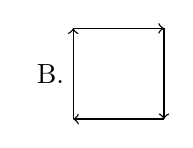
\begin{tikzpicture}[scale=0.72,line width=0.5pt]
\draw[->] (0,0)--(0,1.6);
\draw[->] (0,1.6)--(1.6,1.6);
\draw[->] (1.6,1.6)--(1.6,0);
\draw[->] (1.6,0)--(0,0);
\node at (-0.4,0.8) {B.};
\end{tikzpicture}
&
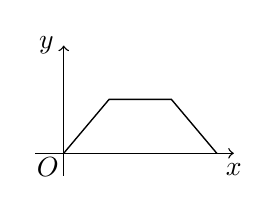
\begin{tikzpicture}[scale=0.72,line width=0.5pt]
\draw[->] (-0.5,0)--(3,0) node[below]{$x$};
\draw[->] (0,-0.4)--(0,1.9) node[left]{$y$};
\draw (0,0)--(0.8,0.95)--(1.9,0.95)--(2.7,0);
\node at (-0.28,-0.25) {$O$};
\end{tikzpicture}
\\
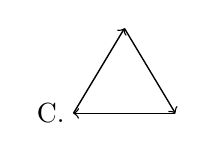
\begin{tikzpicture}[scale=0.72,line width=0.5pt]
\draw[->] (0,0)--(0.9,1.5);
\draw[->] (0.9,1.5)--(1.8,0);
\draw[->] (1.8,0)--(0,0);
\node at (-0.4,0) {C.};
\end{tikzpicture}
&
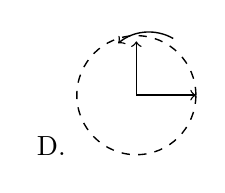
\begin{tikzpicture}[scale=0.72,line width=0.5pt]
\draw[dashed] (1.1,0.9) circle (1.05);
\draw[->] (1.1,0.9)--(2.15,0.9);
\draw[->] (1.1,0.9)--(1.1,1.85);
\draw[->] (1.75,1.9) arc (60:130:0.85);
\node at (-0.4,0) {D.};
\end{tikzpicture}
&
\end{tabular}
\end{center}

\ifanswer
\solbegin
\step{开始离家越来越远，中间离家距离不变，后来离家距离越来越近,}
\step{因此路线 $D$ 符合题意，故选 $D$.}
\solend
\fi

\item 若关于 $x$ 的方程 $ax^2+bx+c=0$（$a>0$）的两个实数根 $x_1$，$x_2$，集合
$S=\{x\mid x>x_1\}$，$T=\{x\mid x>x_2\}$，$P=\{x\mid x<x_1\}$，$Q=\{x\mid x<x_2\}$，则关于 $x$ 的不等式
$ax^2+bx+c>0$ 的解集为\mbox{（\quad）}

\keepwithprev
A. $(S\cap T)\cup(P\cap Q)$\qquad\qquad B. $(S\cap T)\cap(P\cap Q)$

C. $(S\cup T)\cup(P\cup Q)$\qquad\qquad D. $(S\cup T)\cap(P\cup Q)$

\ifanswer
\solbegin
\step{不妨设 $x_1<x_2$，则 $ax^2+bx+c>0$（$a>0$）的解集为 $\{x\mid x<x_1$ 或 $x>x_2\}$,}
\step{$S\cup T=\{x\mid x>x_1\}$，$P\cup Q=\{x\mid x<x_2\}$，$S\cap T=\{x\mid x>x_2\}$,}
\step{$P\cap Q=\{x\mid x<x_1\}$，所以 $(S\cap T)\cup(P\cap Q)=\{x\mid x<x_1$ 或 $x>x_2\}$. 故选 $A$.}
\solend
\fi

\item 已知存在函数 $y=f(x)$ 和 $y=g(x)$ 使得函数 $y=f(g(x))$ 的定义域为 $\R$，且表达式为
$f(g(x))=x^2$，则 $y=g(x)$ 的表达式不可能是\mbox{（\quad）}

\keepwithprev
A. $x^2-3\lvert x\rvert$\qquad B. $x^2+\sqrt{\lvert x\rvert}$\qquad C. $2x-1$\qquad D. $\lvert x\rvert$

\ifanswer
\solbegin
\step{对于选项 A，当 $g(x)=x^2-3\lvert x\rvert$ 时，$g(1)=g(2)=-2$.}
\step{由 $f(g(x))=x^2$ 得 $f(-2)=f(g(1))=1^2=1$，$f(-2)=f(g(2))=2^2=4$，% 原卷两处均作 f(-2)，照录
}
\step{与函数的定义矛盾，所以选项 A 不可能.}
\step{对于选项 B，当 $g(x)=x^2+\sqrt{\lvert x\rvert}$ 时,}
\step{令 $t=x^2+\sqrt{\lvert x\rvert}$，$s=\lvert x\rvert$，$h(s)=s^2+\sqrt s\ (s\geqslant0)$.}
\step{因为函数 $y=s^2$ 在区间 $[0,+\infty)$ 上严格增，函数 $y=\sqrt s$ 在区间 $[0,+\infty)$ 上严格增.}
\step{所以函数 $h(s)=s^2+\sqrt s\ (s\geqslant0)$ 在区间 $[0,+\infty)$ 上严格增.}
\step{故 $s=h^{-1}(t)$，即 $\lvert x\rvert=h^{-1}(t)$，因为 $f(g(x))=x^2=\lvert x\rvert^2$，所以 $f(t)=(h^{-1}(t))^2$,}
\step{即 $f(x)=(h^{-1}(x))^2$，此时 $y=f(g(x))$ 的定义域为 $\R$，故选项 B 可能.}
\step{对于选项 C，当 $g(x)=2x-1$ 时，由 $f(g(x))=x^2$ 得 $f(g(x))=f(2x-1)=x^2$,}
\step{则 $f(x)=\left(\dfrac{x+1}2\right)^2$，此时 $y=f(g(x))$ 的定义域为 $\R$，故选项 C 可能.}
\step{对于选项 D，当 $g(x)=\lvert x\rvert$ 时，由 $f(g(x))=x^2$ 得 $f(g(x))=f(\lvert x\rvert)=x^2$,}
\step{则 $f(x)=x^2\ (x\geqslant0)$，此时 $y=f(g(x))$ 的定义域为 $\R$，故选项 D 可能.}
\step{故选 $A$.}
\solend
\fi

\end{enumerate}

\bigsec{三、解答题}

\begin{enumerate}
\setcounter{enumi}{16}

\item 已知常数 $a\in\R$，集合 $A=\left\{x\,\middle|\,\dfrac{2x+11}{x+2}\geqslant3\right\}$，集合 $B=\{x\mid x^2+2ax-3a^2<0\}$.

（1）若 $a=2$，求 $A\cap B$；

（2）若 $A\cup B=A$，求实数 $a$ 的取值范围.

\ifanswer
\solbegin
\step{（1）$\dfrac{2x+11}{x+2}\geqslant3\Leftrightarrow\dfrac{-x+5}{x+2}\geqslant0\Leftrightarrow\dfrac{x-5}{x+2}\leqslant0\Leftrightarrow
\begin{cases}x+2\neq0\\(x-5)(x+2)\leqslant0\end{cases}$}
\step{$\Leftrightarrow-2<x\leqslant5$，$A=(-2,5]$,}
\step{当 $a=2$ 时，$B=\{x\mid x^2+4x-12<0\}=\{x\mid(x-2)(x+6)<0\}=(-6,2)$,}
\step{$A\cap B=(-2,2)$；}
\step{（2）由 $A\cup B=A$ 得 $B\subseteq A$,}
\step{当 $a=0$ 时，$B=\{x\mid x^2<0\}=\varnothing$，满足题意,}
\step{$x^2+2ax-3a^2=0$ 的两根分别是 $a$ 和 $-3a$,}
\step{当 $a>0$ 时，$B=(-3a,a)$，由题意得 $-2\leqslant-3a<a\leqslant5$，解得 $0<a\leqslant\dfrac23$,}
\step{当 $a<0$ 时，$B=(a,-3a)$，由题意得 $-2\leqslant a<-3a\leqslant5$，解得 $-\dfrac53\leqslant a<0$,}
\step{综上，$-\dfrac53\leqslant a\leqslant\dfrac23$.}
\solend
\fi

\item 某奶茶店今年年初花费 16 万元购买了一台制作冰淇淋的设备，经估算，该设备每年可
为该奶茶店提供 12 万元的总收入. 已知使用 $x$ 年（$x$ 为正整数）所需的各种维护费用总计为
$x^2+2x$ 万元（今年为第一年）.

（1）试问：该奶茶店第几年开始盈利（总收入超过总支出）？

（2）该奶茶店在若干年后要卖出该冰淇淋设备，有以下两种方案：

①当盈利总额达到最大值时，以 1 万元的价格卖出该设备；

②当年均盈利达到最大值时，以 2 万元的价格卖出该设备.

试问哪一种方案较为划算？请说明理由.

\ifanswer
\solbegin
\step{（1）由题意得总收入扣除支出后的纯收入 $y=12x-(x^2+2x+16)$}
\step{$=-x^2+10x-16$，$-x^2+10x-16>0$，解得 $2<x<8$,}
\step{由 $x\in\N^*$，所以从第三年开始盈利；}
\step{（2）方案①：纯收入 $y=-x^2+10x-16=-(x-5)^2+9$,}
\step{则 5 年后盈利总额达到最大值 9 万元，}
\step{以 1 万元的价格卖出该设备，共盈利 10 万元；}
\step{方案②：年均盈利 $z=\dfrac{-x^2+10x-16}{x}=-x+10-\dfrac{16}{x}$,}
\step{由 $x\in\N^*$，$x+\dfrac{16}{x}\geqslant2\sqrt{x\cdot\dfrac{16}{x}}=8$，当且仅当 $x=\dfrac{16}{x}$，即 $x=4$ 时取等号,}
\step{$z=-x+10-\dfrac{16}{x}\leqslant-8+10=2$，当 4 年后年均盈利达到最大值 2 万元时,}
\step{以 2 万元的价格卖出该设备，共盈利 $4\times2+2=10$ 万元.}
\step{两种方案盈利总数一样，但方案②时间短，较为划算.}
\solend
\fi

\item 已知常数 $m\in\R$，$f(x)=\sqrt{\sqrt{x(4-x)}-mx}$.% 原卷题干为双层根号，其解析按单层，见文件头注

（1）证明：对任意的 $m\in\R$，$\{x\mid y=f(x)\}\neq\varnothing$；

（2）若 $[0,2]\subseteq\{x\mid y=f(x)\}$，求实数 $m$ 的取值范围；

（3）若 $\{x\mid y=f(x)\}=[0,3]$，求实数 $m$ 的值.

\ifanswer
\solbegin
\step{（1）$\{x\mid y=f(x)\}=\{x\mid\sqrt{x(4-x)}-mx\geqslant0\}$,}
\step{由 $x(4-x)\geqslant0$ 得 $0\leqslant x\leqslant4$,}
\step{当 $m\leqslant0$ 时，由于 $0\leqslant x\leqslant4$,}
\step{所以 $\sqrt{x(4-x)}-mx\geqslant0$ 对任意 $0\leqslant x\leqslant4$ 恒成立,}
\step{故此时 $\{x\mid y=f(x)\}=\{x\mid0\leqslant x\leqslant4\}$，满足 $\{x\mid y=f(x)\}\neq\varnothing$,}
\step{当 $m>0$ 时，由于 $0\leqslant x\leqslant4$，所以 $mx\geqslant0$，所以 $x(4-x)\geqslant m^2x^2$,}
\step{得 $0\leqslant x\leqslant\dfrac4{1+m^2}$，故此时 $\{x\mid y=f(x)\}=\left\{x\,\middle|\,0\leqslant x\leqslant\dfrac4{1+m^2}\right\}$,}
\step{满足 $\{x\mid y=f(x)\}\neq\varnothing$,}
\step{所以，对任意的 $m\in\R$，$\{x\mid y=f(x)\}\neq\varnothing$；}
\step{（2）由（1）得当 $m\leqslant0$ 时，$\{x\mid y=f(x)\}=\{x\mid0\leqslant x\leqslant4\}$,}
\step{显然满足 $[0,2]\subseteq\{x\mid y=f(x)\}$.}
\step{当 $m>0$ 时，$\{x\mid y=f(x)\}=\left\{x\,\middle|\,0\leqslant x\leqslant\dfrac4{1+m^2}\right\}$,}
\step{由于 $[0,2]\subseteq\{x\mid y=f(x)\}$，所以 $\dfrac4{1+m^2}\geqslant2$，故 $0<m\leqslant1$,}
\step{综上，$m\leqslant1$；}
\step{（3）由于 $\{x\mid y=f(x)\}=[0,3]$,}
\step{所以 $m>0$，$\{x\mid y=f(x)\}=\left\{x\,\middle|\,0\leqslant x\leqslant\dfrac4{1+m^2}\right\}$,}
\step{因此 $\dfrac4{1+m^2}=3$，所以 $m=\dfrac{\sqrt3}3$.}
\solend
\fi

\item 已知函数 $y=f(x)$ 的定义域为 $\R$，其图像是一段连续曲线，对任意的 $a$、$b\in\R$，恒
有 $f(a-b)+f(a+b)=5f(a)\cdot f(b)$，且 $f(0)\neq0$，$f(1)=\dfrac23$.

（1）求 $f(0)$ 和 $f(2)$ 的值；

（2）判断函数 $y=f(x)$ 的奇偶性，并证明；

（3）证明：方程 $f(x)=5$ 在区间 $(2,3)$ 上有解.

\ifanswer
\solbegin
\step{（1）对任意的 $a$、$b\in\R$，恒有 $f(a-b)+f(a+b)=5f(a)\cdot f(b)$,}
\step{且 $f(0)\neq0$，$f(1)=\dfrac23$,}
\step{当 $a=1,b=0$ 时，$f(1)+f(1)=5f(1)\cdot f(0)$，解得 $f(0)=\dfrac25$,}
\step{当 $a=b=1$ 时，$f(0)+f(2)=5f(1)\cdot f(1)$，解得 $f(2)=\dfrac{82}{45}$；}
\step{（2）函数 $y=f(x)$ 为偶函数，证明如下：}
\step{当 $a=0,b=x$ 时，$f(-x)+f(x)=5f(0)\cdot f(x)=2f(x)$,}
\step{则有 $f(-x)=f(x)$，又函数 $y=f(x)$ 的定义域为 $\R$,}
\step{所以函数 $y=f(x)$ 为偶函数.}
\step{（2）$f(2)=\dfrac{82}{45}$% 原卷 (3) 的解答开头误标（2）并重印此行，照录
}
\step{当 $a=2,b=1$ 时，$f(1)+f(3)=5f(2)\cdot f(1)$，解得 $f(3)=\dfrac{146}{27}$,}
\step{函数 $y=f(x)$ 的图像是一段连续曲线，$\dfrac{82}{45}<5<\dfrac{146}{27}$,}
\step{所以存在 $x_0\in(2,3)$，使 $f(x_0)=5$,}
\step{即方程 $f(x)=5$ 在区间 $(2,3)$ 上有解.}
\solend
\fi

\item 若函数 $y=F(x)$ 的定义域为 $D$，且对于任意的 $x_1$、$x_2\in D$，“$F(x_1)=F(x_2)$”的充要
条件是“$x_1=x_2$”，则称函数 $y=F(x)$ 为 $D$ 上的“单值函数”. 对于函数 $y=f(x)$，记
$f^{(1)}(x)=f(x)$，$f^{(2)}(x)=f(f(x))$，$f^{(3)}(x)=f(f(f(x)))$，$\cdots$，$f^{(n+1)}(x)=f(f^{(n)}(x))$，其
中 $n=1,2,3,\cdots$，并对任意的 $A\subseteq D$，记集合 $f^{(n)}(A)=\left\{f^{(n)}(x)\mid x\in A\right\}$，并规定
$f^{(n)}(\varnothing)=\varnothing$.

（1）若 $f(x)=2x+1$，函数 $y=f(x)$ 的定义域为 $\R$，求 $f^{(2)}([0,1])$ 和 $f^{(3)}([0,1])$；

（2）若函数 $y=f(x)$ 的定义域为 $D$，且存在正整数 $m$，使得对任意的 $x\in D$，$f^{(m)}(x)=x$，
求证：函数 $y=f(x)$ 为 $D$ 上的“单值函数”；

（3）设 $a\in(0,1)$，若函数 $y=f(x)$ 的定义域为 $(0,1]$，且表达式为：
\[f(x)=\begin{cases}x+(1-a),&0<x\leqslant a,\\x-a,&a<x\leqslant1\end{cases}\]
判断 $y=f(x)$ 是否为 $(0,1]$ 上的“单值函数”，并证明对任
意的区间 $I\subseteq(0,1]$，存在正整数 $k$，使得 $f^{(k)}(I)\cap I\neq\varnothing$.

\ifanswer
\solbegin
\step{（1）当 $x\in[0,1]$ 时，$2x+1\in[1,3]$，所以 $f^{(1)}([0,1])=[1,3]$,}
\step{当 $x\in[1,3]$ 时，$2x+1\in[3,7]$，所以 $f^{(2)}([0,1])=[3,7]$,}
\step{当 $x\in[3,7]$ 时，$2x+1\in[7,15]$，所以 $f^{(3)}([0,1])=[7,15]$；}
\step{（2）由已知单值函数的定义可以改写为：若函数 $y=F(x)$ 的定义域为 $D$,}
\step{且对于任意的 $x_1$、$x_2\in D$，“$F(x_1)\neq F(x_2)$”的充要条件是“$x_1\neq x_2$”,}
\step{则称函数 $y=F(x)$ 为 $D$ 上的“单值函数.}
\step{假设 $f(x)$ 不是 $D$ 上的单值函数,}
\step{则存在 $x_1,x_2\in D,x_1\neq x_2$，$f(x_1)=f(x_2)$ 成立，即 $f^{(1)}(x_1)=f^{(1)}(x_2)$,}
\step{于是 $f\left[f^{(1)}(x_1)\right]=f\left[f^{(1)}(x_2)\right]$，即 $f^{(2)}(x_1)=f^{(2)}(x_2)$,}
\step{依此类推，得 $f^{(m)}(x_1)=f^{(m)}(x_2)$,}
\step{但由题意得 $f^{(m)}(x)=x$，因此 $f^{(2)}(x_1)=x_2$，$f^{(2)}(x_2)=x_2$，而 $x_1\neq x_2$,}
\step{因此 $f^{(m)}(x_1)\neq f^{(m)}(x_2)$，这样得出了矛盾的结论，所以假设不成立,}
\step{即 $f(x)$ 是 $D$ 上的单值函数；}
\step{（3）由新定义得 $f(x)=x+(1-a)$ 是单值函数，$f(x)=x-a$ 也是单值函数,}
\step{$0<a<1$，则 $0<1-a<1$,}
\step{又 $0<x\leqslant a$ 时，$f(x)=x+(1-a)\in(1-a,1]$,}
\step{$a<x\leqslant1$ 时，$f(x)=x-a\in(0,1-a]$，又 $(0,1-a]\cap(1-a,1]=\varnothing$,}
\step{因此对任意的 $x_1,x_2\in(0,1],x_1\neq x_2\Leftrightarrow f(x_1)\neq f(x_2)$,}
\step{所以 $y=f(x)$ 是 $(0,1]$ 上的“单值函数”,}
\step{对于任意的有限的区间 $I$，记 $\lvert I\rvert$ 表示区间 $I$ 的长度,}
\step{如果一个集合 $A$ 是若干个区间的并集,}
\step{则 $\lvert A\rvert$ 等于组成它的所有区间的长度之和,}
\step{对于任意的区间 $I\subseteq(0,1]$，$x\in I$，$f(I)=\{f(x)\mid x\in T\}$,}
\step{不妨设 $I=(s,t)$，$(0<s<t\leqslant1)$，$\lvert T\rvert=t-s$,}
\step{若 $(s,t)\subseteq(0,a]$，则 $f(I)=(s+1-a,t+1-a)$，$\lvert f(T)\rvert=t-s$,}
\step{若 $(s,t)\subseteq(a,1]$，则 $f(I)=(s-a,t-a)$，$\lvert f(T)\rvert=t-s$,}
\step{若 $a\in(s,t)$，则 $f(I)=(s+1-a,1]\cup(0,t-a)$,}
\step{$\lvert f(T)\rvert=1-(s+1-a)+(t-a)-0=t-s$，所以 $\lvert f(I)\rvert=\lvert I\rvert$,}
\step{对于任意的区间 $I\subseteq(0,1]$，显然存在正整数 $n$，使得 $n\lvert I\rvert>1$,}
\step{因此在 $f^{(0)}(I),f^{(1)}(I),f^{(2)}(I),\cdots,f^{(n)}(I)$（它们的长度和大于 1）中,}
\step{必然存在正整数 $m,l\ (m>l)$，使得 $f^{(m)}(I)\cap f^{(l)}(I)\neq\varnothing$,}
\step{因此必存在 $x,y\in I$，使得 $f^{(m)}(x)=f^{(l)}(y)$,}
\step{又 $y=f(x)$ 是 $(0,1]$ 上的单值函数,}
\step{所以 $f^{(m-1)}(x)=f^{(l-1)}(y)$，$f^{(m-2)}(x)=f^{(l-2)}(y)$，$\cdots$，$f^{(m-l)}(x)=y$,}
\step{这表示 $f^{(m-l)}(I)\cap I\neq\varnothing$，取 $k=m-l$,}
\step{所以对任意的区间 $I\subseteq(0,1]$，存在正整数 $k$，使得 $f^{(k)}(I)\cap I\neq\varnothing$.}
\solend
\fi

\end{enumerate}

\end{document}
"
% 紧凑版：xelatex "\def\iscompact{1}% 高一106_复旦附中_周末作业11期中复习.tex
%   —— 高一上数学“2026-2027 年复旦附中高一上周末作业 11 期中复习”（试卷版/答案版）
% 试卷版：xelatex 高一106_复旦附中_周末作业11期中复习.tex
% 答案版：xelatex "\def\isanswer{1}\input{高一106_复旦附中_周末作业11期中复习.tex}"
% 紧凑版：xelatex "\def\iscompact{1}\input{高一106_复旦附中_周末作业11期中复习.tex}"
%
% 原始材料：微信公众号“魔都数学加油站”文章，作者破晓，2026-11-03 17:19 发布；
% 连载“27学年高一106”，原文标题“27学年高一106——2026-2027年上海市复旦附中高一上周末作业11期中复习”；
% 原文链接：https://mp.weixin.qq.com/s/O3N1S8hA2awUzsOnRvCI-w。
% 正文为 9 张 PNG 页（第 1—2、4—8 页 4762×6735，第 3、9 页 2560×3620），题目下印有【解析】，为讲评版。
% 题目、解析均据原图转录；卷面水印及公众号页脚未录入。
% 第 14 题的四幅路线图选项与题干右侧的 $y$-$x$ 图像按原图形状用 TikZ 重绘。
%
% 卷首标题：原卷印作“2026-2027 年复旦附中高一上周末作业 11 期中复习”（公众号标题中的“上海市”
% 卷面标题行没有，本稿照卷面），年份区间按全稿惯例排 en dash；原卷未印副标题，本稿按题目内容
% 标为“集合与常用逻辑用语、不等式、函数”（期中复习跨三章）。
%
% 与原卷的排版差异：
%   ① 原文从第 3 题起，填空题编号为 3—12、选择题为 13—16、解答题为 17—21，本稿保留原题号；
%   ② 原卷每题下直接印【解析】，本稿按全稿惯例将解析置于答案版；第 13 题原卷把答案“$A$”
%      印在题干括号内且无【解析】，本稿试卷版留空、答案版提 \ans{}；
%   ③ 原卷未印副标题，本稿按“知识模块”口径补出；
%   ④ 原卷填空横线按全稿惯例排为 \blankline[4.4em]；解答题按惯例加 \ansspace；选择题括号排
%      \mbox{（\quad）}、选项段前按惯例加 \keepwithprev；
%   ⑤ 原卷数集排粗体 $\mathbf{R}$，按全稿惯例改 \R；
%   ⑥ 第 11 题题干“集　合　X”三字原卷字距拉得很开（铅字排版的空隙），本稿按正常字距排。
%
% 原卷存疑：第 16 题解析第二行原卷作“$f(-2)=f(g(1))=1^2=1$，$f(-2)=f(g(2))=2^2=4$”
% （两个都写 $f(-2)$；按 $g(1)=g(2)=-2$，两处相等正构成矛盾，但第二处按复合应写
% $f(g(2))=f(-2)$），本稿照录。第 19 题题干 $f(x)$ 为**双层根号**
% $\sqrt{\sqrt{x(4-x)}-mx}$，而解析 (1) 首行只写单层 $\sqrt{x(4-x)}-mx\geqslant0$
% （其后推导均按单层），原卷题干与解析不一致，各照录。
% 第 20 题解析 (3) 的解答开头原卷误标“（2）”并重印 $f(2)=\dfrac{82}{45}$ 一行，照录。
%
% 行数核对：逐题数 \step/\stepm 条数，合计 132 条（Q3：2；Q4：3；Q5：3；Q6：1；Q7：3；
% Q8：5；Q9：2；Q10：2；Q11：3；Q12：2；Q13：0；Q14：2；Q15：3；Q16：14；Q17：10；
% Q18：11；Q19：17；Q20：13；Q21：36），与原卷印刷行逐题相等。第 13 题括号内印答案、
% 无解析，提 \ans{}，不计入 \step 账。
%
\documentclass[a4paper,11pt]{article}
\usepackage{common}

\begin{document}

\examtitlest[3]{2026--2027 年复旦附中高一上周末作业 11 期中复习}{集合与常用逻辑用语、不等式、函数}

\bigsec{一、填空题}

\begin{enumerate}
\setcounter{enumi}{2}

\item 若关于 $x$ 的不等式组
$\begin{cases}2x+3>0\\x+3a<0\end{cases}$
的解集非空，则满足条件的最大整数 $a=$\blankline[4.4em].

\ifanswer
\solbegin
\step{由
$\begin{cases}2x+3>0\\x+3a<0\end{cases}$
得
$\begin{cases}x>-\dfrac32\\x<-3a\end{cases}$，
要使不等式组
$\begin{cases}2x+3>0\\x+3a<0\end{cases}$
的解集非空，}
\step{须 $-3a>-\dfrac32$，即 $a<\dfrac12$，故满足条件的最大整数 $a=0$.}
\solend
\fi

\item 若关于 $x$ 的不等式 $\lvert x-366\rvert+\lvert x-500\rvert\leqslant a$ 的解集非空，则 $a$ 的取值范围是\blankline[4.4em].

\ifanswer
\solbegin
\step{$\lvert x-366\rvert+\lvert x-500\rvert\geqslant\lvert x-366-(x-500)\rvert=134$,}
\step{当且仅当 $366\leqslant x\leqslant500$ 时取等号，所以 $\lvert x-366\rvert+\lvert x-500\rvert$ 的最小值为 134,}
\step{从而 $a\geqslant134$. 故 $a$ 的取值范围是 $[134,+\infty)$.}
\solend
\fi

\item 设集合 $A=\{1,2,3,4\}$，$B=\{1,2\}$，若 $C\subseteq A$ 且 $B\cap C\neq\varnothing$，则所有满足条件的集合 $C$ 的个数为\blankline[4.4em].

\ifanswer
\solbegin
\step{按题意，集合 $C$ 是 $A$ 的子集，且与 $B$ 的交集不为空集,}
\step{集合 $A$ 的子集有 $2^4=16$ 个，其中与 $B$ 的交集为空集的子集，即 $\{3,4\}$ 的子集,}
\step{有 $2^2=4$ 个，故满足题意的集合 $C$ 的个数为 $16-4=12$.}
\solend
\fi

\item 函数 $f(x)=\lvert x^2-3x+2\rvert$ 的单调增区间为\blankline[4.4em].

\ifanswer
\solbegin
\step{观察图像得函数 $f(x)=\lvert x^2-3x+2\rvert$ 的严格增区间为 $\left(1,\dfrac32\right),(2,+\infty)$.}
\solend
\fi

\item 已知 $f(x)=\sqrt{mx^2-mx+1}$，若函数 $y=f(x)$ 的定义域为 $\R$，则实数 $m$ 的取值范围为\blankline[4.4em].

\ifanswer
\solbegin
\step{当 $m=0$ 时，$f(x)=1$ 满足题意,}
\step{当 $m>0$ 时，$\Delta=m^2-4m\leqslant0$，所以 $0<m\leqslant4$,}
\step{故实数 $m$ 的取值范围为 $[0,4]$.}
\solend
\fi

\item 已知 $T$ 是方程 $x^2+px+q=0$（$p^2-4q>0$）的解集，$A=\{1,3,5,7,9\}$，$B=\{1,4,7,10\}$ 且 $T\cap A=\varnothing$，$T\cap B=T$，则 $p+q=$\blankline[4.4em].

\ifanswer
\solbegin
\step{对方程 $x^2+px+q=0$（$p^2-4q>0$），显然有两个根，故集合 $T$ 中有两个元素；}
\step{因为 $T\cap B=T$，所以 $T$ 中的两个元素一定在集合 $B$ 中；}
\step{又因为 $T\cap A=\varnothing$，故 $T$ 中的所有元素都不在 $A$ 中；}
\step{综上，$T$ 中的元素一定是 4 和 10，由根与系数的关系得 $14=-p,40=q$,}
\step{则 $p+q=26$.}
\solend
\fi

\item 已知正实数 $a$、$b$ 满足 $a+b=a^2+b^2$，则 $\dfrac1a+\dfrac1b$ 的最小值为\blankline[4.4em].

\ifanswer
\solbegin
\step{由已知 $\dfrac1a+\dfrac1b=\dfrac{a+b}{ab}=\dfrac{a^2+b^2}{ab}=\dfrac ab+\dfrac ba\geqslant2\sqrt{\dfrac ab\cdot\dfrac ba}=2$,}
\step{当且仅当 $\dfrac ba=\dfrac ab$，即 $a=b=1$ 时取等号，故 $\dfrac1a+\dfrac1b$ 的最小值为 $1$.}
\solend
\fi

\item 已知 $a$、$b$、$c$ 为实数，且 $a^2+c^2=64$，$b^2+c^2=100$，则 $a^2+b^2$ 的取值范围是\blankline[4.4em].

\ifanswer
\solbegin
\step{由题意得
$\begin{cases}a^2=64-c^2\\b^2=100-c^2\end{cases}\Rightarrow a^2+b^2=164-2c^2$，
其中 $0\leqslant c^2\leqslant64$,}
\step{因此 $a^2+b^2$ 的取值范围是 $[36,164]$.}
\solend
\fi

\item 设 $U$ 为全集，对集合 $X$，$Y$，定义运算“$*$”，$M*N=\overline{M\cap N}$. 已知全集
$U=\{1,2,3,4,5,6,7,8\}$，集合 $X=\{1,2,3\}$，$Y=\{3,4,5\}$，$Z=\{2,4,7\}$，则
$(X*Y)*Z=$\blankline[4.4em].% 原卷“集 合 X”三字字距拉得很开，本稿按正常字距排

\ifanswer
\solbegin
\step{因为集合 $U=\{1,2,3,4,5,6,7,8\}$，$X=\{1,2,3\}$，$Y=\{3,4,5\}$，$Z=\{2,4,7\}$,}
\step{所以 $X\cap Y=\{3\}$，则 $X*Y=\overline{X\cap Y}=\{1,2,4,5,6,7,8\}$,}
\step{又 $\{1,2,4,5,6,7,8\}\cap\{2,4,7\}=\{2,4,7\}$，所以 $(X*Y)*Z=\{1,3,5,6,8\}$.}
\solend
\fi

\item 已知一个奇函数 $y=f(x)$ 与一个偶函数 $y=g(x)$ 的和为函数 $y=\sqrt{x^2-3x+6}$，则 $f(3)=$\blankline[4.4em].

\ifanswer
\solbegin
\step{记 $h(x)=\sqrt{x^2-3x+6}$，由题意得
$\begin{cases}f(3)+g(3)=h(3)=\sqrt6\\f(-3)+g(-3)=h(-3)=2\sqrt6\end{cases}$,}
\step{又 $f(-3)=-f(3)$，$g(-3)=g(3)$，解得 $f(3)=-\dfrac{\sqrt6}2$.}
\solend
\fi

\end{enumerate}

\bigsec{二、选择题}

\begin{enumerate}
\setcounter{enumi}{12}

\item 已知 $a>b$ 均为正实数，则“$c>d$”是“$a+c>b+d$”的\mbox{（\quad）}条件% 原卷把答案“A”印在题干括号内、无【解析】

\keepwithprev
A. 充分非必要\qquad\qquad B. 必要不充分

C. 充分必要\qquad\qquad\qquad D. 既非充分又非必要

\ifanswer
\ans{$A$}
\fi

\item 如图是肖老师以恒定的速率夜跑时的离家距离 $(y)$ 与跑步时间 $(x)$ 之间的函数的图像，
则肖老师跑步的路线可能是\mbox{（\quad）}

\keepwithprev
\begin{center}
\begin{tabular}{ccc}
\begin{tikzpicture}[scale=0.72,line width=0.5pt]
\draw[->] (0,0)--(1.1,1.1);
\draw[->] (1.1,1.1)--(2.7,1.1);
\draw[->] (2.7,1.1)--(3.8,0);
\node at (-0.4,0) {A.};
\end{tikzpicture}
&
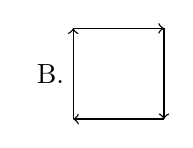
\begin{tikzpicture}[scale=0.72,line width=0.5pt]
\draw[->] (0,0)--(0,1.6);
\draw[->] (0,1.6)--(1.6,1.6);
\draw[->] (1.6,1.6)--(1.6,0);
\draw[->] (1.6,0)--(0,0);
\node at (-0.4,0.8) {B.};
\end{tikzpicture}
&
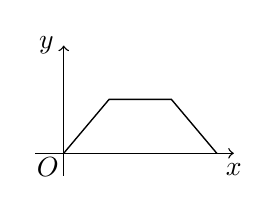
\begin{tikzpicture}[scale=0.72,line width=0.5pt]
\draw[->] (-0.5,0)--(3,0) node[below]{$x$};
\draw[->] (0,-0.4)--(0,1.9) node[left]{$y$};
\draw (0,0)--(0.8,0.95)--(1.9,0.95)--(2.7,0);
\node at (-0.28,-0.25) {$O$};
\end{tikzpicture}
\\
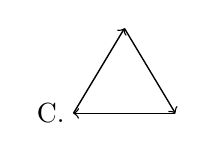
\begin{tikzpicture}[scale=0.72,line width=0.5pt]
\draw[->] (0,0)--(0.9,1.5);
\draw[->] (0.9,1.5)--(1.8,0);
\draw[->] (1.8,0)--(0,0);
\node at (-0.4,0) {C.};
\end{tikzpicture}
&
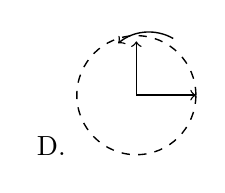
\begin{tikzpicture}[scale=0.72,line width=0.5pt]
\draw[dashed] (1.1,0.9) circle (1.05);
\draw[->] (1.1,0.9)--(2.15,0.9);
\draw[->] (1.1,0.9)--(1.1,1.85);
\draw[->] (1.75,1.9) arc (60:130:0.85);
\node at (-0.4,0) {D.};
\end{tikzpicture}
&
\end{tabular}
\end{center}

\ifanswer
\solbegin
\step{开始离家越来越远，中间离家距离不变，后来离家距离越来越近,}
\step{因此路线 $D$ 符合题意，故选 $D$.}
\solend
\fi

\item 若关于 $x$ 的方程 $ax^2+bx+c=0$（$a>0$）的两个实数根 $x_1$，$x_2$，集合
$S=\{x\mid x>x_1\}$，$T=\{x\mid x>x_2\}$，$P=\{x\mid x<x_1\}$，$Q=\{x\mid x<x_2\}$，则关于 $x$ 的不等式
$ax^2+bx+c>0$ 的解集为\mbox{（\quad）}

\keepwithprev
A. $(S\cap T)\cup(P\cap Q)$\qquad\qquad B. $(S\cap T)\cap(P\cap Q)$

C. $(S\cup T)\cup(P\cup Q)$\qquad\qquad D. $(S\cup T)\cap(P\cup Q)$

\ifanswer
\solbegin
\step{不妨设 $x_1<x_2$，则 $ax^2+bx+c>0$（$a>0$）的解集为 $\{x\mid x<x_1$ 或 $x>x_2\}$,}
\step{$S\cup T=\{x\mid x>x_1\}$，$P\cup Q=\{x\mid x<x_2\}$，$S\cap T=\{x\mid x>x_2\}$,}
\step{$P\cap Q=\{x\mid x<x_1\}$，所以 $(S\cap T)\cup(P\cap Q)=\{x\mid x<x_1$ 或 $x>x_2\}$. 故选 $A$.}
\solend
\fi

\item 已知存在函数 $y=f(x)$ 和 $y=g(x)$ 使得函数 $y=f(g(x))$ 的定义域为 $\R$，且表达式为
$f(g(x))=x^2$，则 $y=g(x)$ 的表达式不可能是\mbox{（\quad）}

\keepwithprev
A. $x^2-3\lvert x\rvert$\qquad B. $x^2+\sqrt{\lvert x\rvert}$\qquad C. $2x-1$\qquad D. $\lvert x\rvert$

\ifanswer
\solbegin
\step{对于选项 A，当 $g(x)=x^2-3\lvert x\rvert$ 时，$g(1)=g(2)=-2$.}
\step{由 $f(g(x))=x^2$ 得 $f(-2)=f(g(1))=1^2=1$，$f(-2)=f(g(2))=2^2=4$，% 原卷两处均作 f(-2)，照录
}
\step{与函数的定义矛盾，所以选项 A 不可能.}
\step{对于选项 B，当 $g(x)=x^2+\sqrt{\lvert x\rvert}$ 时,}
\step{令 $t=x^2+\sqrt{\lvert x\rvert}$，$s=\lvert x\rvert$，$h(s)=s^2+\sqrt s\ (s\geqslant0)$.}
\step{因为函数 $y=s^2$ 在区间 $[0,+\infty)$ 上严格增，函数 $y=\sqrt s$ 在区间 $[0,+\infty)$ 上严格增.}
\step{所以函数 $h(s)=s^2+\sqrt s\ (s\geqslant0)$ 在区间 $[0,+\infty)$ 上严格增.}
\step{故 $s=h^{-1}(t)$，即 $\lvert x\rvert=h^{-1}(t)$，因为 $f(g(x))=x^2=\lvert x\rvert^2$，所以 $f(t)=(h^{-1}(t))^2$,}
\step{即 $f(x)=(h^{-1}(x))^2$，此时 $y=f(g(x))$ 的定义域为 $\R$，故选项 B 可能.}
\step{对于选项 C，当 $g(x)=2x-1$ 时，由 $f(g(x))=x^2$ 得 $f(g(x))=f(2x-1)=x^2$,}
\step{则 $f(x)=\left(\dfrac{x+1}2\right)^2$，此时 $y=f(g(x))$ 的定义域为 $\R$，故选项 C 可能.}
\step{对于选项 D，当 $g(x)=\lvert x\rvert$ 时，由 $f(g(x))=x^2$ 得 $f(g(x))=f(\lvert x\rvert)=x^2$,}
\step{则 $f(x)=x^2\ (x\geqslant0)$，此时 $y=f(g(x))$ 的定义域为 $\R$，故选项 D 可能.}
\step{故选 $A$.}
\solend
\fi

\end{enumerate}

\bigsec{三、解答题}

\begin{enumerate}
\setcounter{enumi}{16}

\item 已知常数 $a\in\R$，集合 $A=\left\{x\,\middle|\,\dfrac{2x+11}{x+2}\geqslant3\right\}$，集合 $B=\{x\mid x^2+2ax-3a^2<0\}$.

（1）若 $a=2$，求 $A\cap B$；

（2）若 $A\cup B=A$，求实数 $a$ 的取值范围.

\ifanswer
\solbegin
\step{（1）$\dfrac{2x+11}{x+2}\geqslant3\Leftrightarrow\dfrac{-x+5}{x+2}\geqslant0\Leftrightarrow\dfrac{x-5}{x+2}\leqslant0\Leftrightarrow
\begin{cases}x+2\neq0\\(x-5)(x+2)\leqslant0\end{cases}$}
\step{$\Leftrightarrow-2<x\leqslant5$，$A=(-2,5]$,}
\step{当 $a=2$ 时，$B=\{x\mid x^2+4x-12<0\}=\{x\mid(x-2)(x+6)<0\}=(-6,2)$,}
\step{$A\cap B=(-2,2)$；}
\step{（2）由 $A\cup B=A$ 得 $B\subseteq A$,}
\step{当 $a=0$ 时，$B=\{x\mid x^2<0\}=\varnothing$，满足题意,}
\step{$x^2+2ax-3a^2=0$ 的两根分别是 $a$ 和 $-3a$,}
\step{当 $a>0$ 时，$B=(-3a,a)$，由题意得 $-2\leqslant-3a<a\leqslant5$，解得 $0<a\leqslant\dfrac23$,}
\step{当 $a<0$ 时，$B=(a,-3a)$，由题意得 $-2\leqslant a<-3a\leqslant5$，解得 $-\dfrac53\leqslant a<0$,}
\step{综上，$-\dfrac53\leqslant a\leqslant\dfrac23$.}
\solend
\fi

\item 某奶茶店今年年初花费 16 万元购买了一台制作冰淇淋的设备，经估算，该设备每年可
为该奶茶店提供 12 万元的总收入. 已知使用 $x$ 年（$x$ 为正整数）所需的各种维护费用总计为
$x^2+2x$ 万元（今年为第一年）.

（1）试问：该奶茶店第几年开始盈利（总收入超过总支出）？

（2）该奶茶店在若干年后要卖出该冰淇淋设备，有以下两种方案：

①当盈利总额达到最大值时，以 1 万元的价格卖出该设备；

②当年均盈利达到最大值时，以 2 万元的价格卖出该设备.

试问哪一种方案较为划算？请说明理由.

\ifanswer
\solbegin
\step{（1）由题意得总收入扣除支出后的纯收入 $y=12x-(x^2+2x+16)$}
\step{$=-x^2+10x-16$，$-x^2+10x-16>0$，解得 $2<x<8$,}
\step{由 $x\in\N^*$，所以从第三年开始盈利；}
\step{（2）方案①：纯收入 $y=-x^2+10x-16=-(x-5)^2+9$,}
\step{则 5 年后盈利总额达到最大值 9 万元，}
\step{以 1 万元的价格卖出该设备，共盈利 10 万元；}
\step{方案②：年均盈利 $z=\dfrac{-x^2+10x-16}{x}=-x+10-\dfrac{16}{x}$,}
\step{由 $x\in\N^*$，$x+\dfrac{16}{x}\geqslant2\sqrt{x\cdot\dfrac{16}{x}}=8$，当且仅当 $x=\dfrac{16}{x}$，即 $x=4$ 时取等号,}
\step{$z=-x+10-\dfrac{16}{x}\leqslant-8+10=2$，当 4 年后年均盈利达到最大值 2 万元时,}
\step{以 2 万元的价格卖出该设备，共盈利 $4\times2+2=10$ 万元.}
\step{两种方案盈利总数一样，但方案②时间短，较为划算.}
\solend
\fi

\item 已知常数 $m\in\R$，$f(x)=\sqrt{\sqrt{x(4-x)}-mx}$.% 原卷题干为双层根号，其解析按单层，见文件头注

（1）证明：对任意的 $m\in\R$，$\{x\mid y=f(x)\}\neq\varnothing$；

（2）若 $[0,2]\subseteq\{x\mid y=f(x)\}$，求实数 $m$ 的取值范围；

（3）若 $\{x\mid y=f(x)\}=[0,3]$，求实数 $m$ 的值.

\ifanswer
\solbegin
\step{（1）$\{x\mid y=f(x)\}=\{x\mid\sqrt{x(4-x)}-mx\geqslant0\}$,}
\step{由 $x(4-x)\geqslant0$ 得 $0\leqslant x\leqslant4$,}
\step{当 $m\leqslant0$ 时，由于 $0\leqslant x\leqslant4$,}
\step{所以 $\sqrt{x(4-x)}-mx\geqslant0$ 对任意 $0\leqslant x\leqslant4$ 恒成立,}
\step{故此时 $\{x\mid y=f(x)\}=\{x\mid0\leqslant x\leqslant4\}$，满足 $\{x\mid y=f(x)\}\neq\varnothing$,}
\step{当 $m>0$ 时，由于 $0\leqslant x\leqslant4$，所以 $mx\geqslant0$，所以 $x(4-x)\geqslant m^2x^2$,}
\step{得 $0\leqslant x\leqslant\dfrac4{1+m^2}$，故此时 $\{x\mid y=f(x)\}=\left\{x\,\middle|\,0\leqslant x\leqslant\dfrac4{1+m^2}\right\}$,}
\step{满足 $\{x\mid y=f(x)\}\neq\varnothing$,}
\step{所以，对任意的 $m\in\R$，$\{x\mid y=f(x)\}\neq\varnothing$；}
\step{（2）由（1）得当 $m\leqslant0$ 时，$\{x\mid y=f(x)\}=\{x\mid0\leqslant x\leqslant4\}$,}
\step{显然满足 $[0,2]\subseteq\{x\mid y=f(x)\}$.}
\step{当 $m>0$ 时，$\{x\mid y=f(x)\}=\left\{x\,\middle|\,0\leqslant x\leqslant\dfrac4{1+m^2}\right\}$,}
\step{由于 $[0,2]\subseteq\{x\mid y=f(x)\}$，所以 $\dfrac4{1+m^2}\geqslant2$，故 $0<m\leqslant1$,}
\step{综上，$m\leqslant1$；}
\step{（3）由于 $\{x\mid y=f(x)\}=[0,3]$,}
\step{所以 $m>0$，$\{x\mid y=f(x)\}=\left\{x\,\middle|\,0\leqslant x\leqslant\dfrac4{1+m^2}\right\}$,}
\step{因此 $\dfrac4{1+m^2}=3$，所以 $m=\dfrac{\sqrt3}3$.}
\solend
\fi

\item 已知函数 $y=f(x)$ 的定义域为 $\R$，其图像是一段连续曲线，对任意的 $a$、$b\in\R$，恒
有 $f(a-b)+f(a+b)=5f(a)\cdot f(b)$，且 $f(0)\neq0$，$f(1)=\dfrac23$.

（1）求 $f(0)$ 和 $f(2)$ 的值；

（2）判断函数 $y=f(x)$ 的奇偶性，并证明；

（3）证明：方程 $f(x)=5$ 在区间 $(2,3)$ 上有解.

\ifanswer
\solbegin
\step{（1）对任意的 $a$、$b\in\R$，恒有 $f(a-b)+f(a+b)=5f(a)\cdot f(b)$,}
\step{且 $f(0)\neq0$，$f(1)=\dfrac23$,}
\step{当 $a=1,b=0$ 时，$f(1)+f(1)=5f(1)\cdot f(0)$，解得 $f(0)=\dfrac25$,}
\step{当 $a=b=1$ 时，$f(0)+f(2)=5f(1)\cdot f(1)$，解得 $f(2)=\dfrac{82}{45}$；}
\step{（2）函数 $y=f(x)$ 为偶函数，证明如下：}
\step{当 $a=0,b=x$ 时，$f(-x)+f(x)=5f(0)\cdot f(x)=2f(x)$,}
\step{则有 $f(-x)=f(x)$，又函数 $y=f(x)$ 的定义域为 $\R$,}
\step{所以函数 $y=f(x)$ 为偶函数.}
\step{（2）$f(2)=\dfrac{82}{45}$% 原卷 (3) 的解答开头误标（2）并重印此行，照录
}
\step{当 $a=2,b=1$ 时，$f(1)+f(3)=5f(2)\cdot f(1)$，解得 $f(3)=\dfrac{146}{27}$,}
\step{函数 $y=f(x)$ 的图像是一段连续曲线，$\dfrac{82}{45}<5<\dfrac{146}{27}$,}
\step{所以存在 $x_0\in(2,3)$，使 $f(x_0)=5$,}
\step{即方程 $f(x)=5$ 在区间 $(2,3)$ 上有解.}
\solend
\fi

\item 若函数 $y=F(x)$ 的定义域为 $D$，且对于任意的 $x_1$、$x_2\in D$，“$F(x_1)=F(x_2)$”的充要
条件是“$x_1=x_2$”，则称函数 $y=F(x)$ 为 $D$ 上的“单值函数”. 对于函数 $y=f(x)$，记
$f^{(1)}(x)=f(x)$，$f^{(2)}(x)=f(f(x))$，$f^{(3)}(x)=f(f(f(x)))$，$\cdots$，$f^{(n+1)}(x)=f(f^{(n)}(x))$，其
中 $n=1,2,3,\cdots$，并对任意的 $A\subseteq D$，记集合 $f^{(n)}(A)=\left\{f^{(n)}(x)\mid x\in A\right\}$，并规定
$f^{(n)}(\varnothing)=\varnothing$.

（1）若 $f(x)=2x+1$，函数 $y=f(x)$ 的定义域为 $\R$，求 $f^{(2)}([0,1])$ 和 $f^{(3)}([0,1])$；

（2）若函数 $y=f(x)$ 的定义域为 $D$，且存在正整数 $m$，使得对任意的 $x\in D$，$f^{(m)}(x)=x$，
求证：函数 $y=f(x)$ 为 $D$ 上的“单值函数”；

（3）设 $a\in(0,1)$，若函数 $y=f(x)$ 的定义域为 $(0,1]$，且表达式为：
\[f(x)=\begin{cases}x+(1-a),&0<x\leqslant a,\\x-a,&a<x\leqslant1\end{cases}\]
判断 $y=f(x)$ 是否为 $(0,1]$ 上的“单值函数”，并证明对任
意的区间 $I\subseteq(0,1]$，存在正整数 $k$，使得 $f^{(k)}(I)\cap I\neq\varnothing$.

\ifanswer
\solbegin
\step{（1）当 $x\in[0,1]$ 时，$2x+1\in[1,3]$，所以 $f^{(1)}([0,1])=[1,3]$,}
\step{当 $x\in[1,3]$ 时，$2x+1\in[3,7]$，所以 $f^{(2)}([0,1])=[3,7]$,}
\step{当 $x\in[3,7]$ 时，$2x+1\in[7,15]$，所以 $f^{(3)}([0,1])=[7,15]$；}
\step{（2）由已知单值函数的定义可以改写为：若函数 $y=F(x)$ 的定义域为 $D$,}
\step{且对于任意的 $x_1$、$x_2\in D$，“$F(x_1)\neq F(x_2)$”的充要条件是“$x_1\neq x_2$”,}
\step{则称函数 $y=F(x)$ 为 $D$ 上的“单值函数.}
\step{假设 $f(x)$ 不是 $D$ 上的单值函数,}
\step{则存在 $x_1,x_2\in D,x_1\neq x_2$，$f(x_1)=f(x_2)$ 成立，即 $f^{(1)}(x_1)=f^{(1)}(x_2)$,}
\step{于是 $f\left[f^{(1)}(x_1)\right]=f\left[f^{(1)}(x_2)\right]$，即 $f^{(2)}(x_1)=f^{(2)}(x_2)$,}
\step{依此类推，得 $f^{(m)}(x_1)=f^{(m)}(x_2)$,}
\step{但由题意得 $f^{(m)}(x)=x$，因此 $f^{(2)}(x_1)=x_2$，$f^{(2)}(x_2)=x_2$，而 $x_1\neq x_2$,}
\step{因此 $f^{(m)}(x_1)\neq f^{(m)}(x_2)$，这样得出了矛盾的结论，所以假设不成立,}
\step{即 $f(x)$ 是 $D$ 上的单值函数；}
\step{（3）由新定义得 $f(x)=x+(1-a)$ 是单值函数，$f(x)=x-a$ 也是单值函数,}
\step{$0<a<1$，则 $0<1-a<1$,}
\step{又 $0<x\leqslant a$ 时，$f(x)=x+(1-a)\in(1-a,1]$,}
\step{$a<x\leqslant1$ 时，$f(x)=x-a\in(0,1-a]$，又 $(0,1-a]\cap(1-a,1]=\varnothing$,}
\step{因此对任意的 $x_1,x_2\in(0,1],x_1\neq x_2\Leftrightarrow f(x_1)\neq f(x_2)$,}
\step{所以 $y=f(x)$ 是 $(0,1]$ 上的“单值函数”,}
\step{对于任意的有限的区间 $I$，记 $\lvert I\rvert$ 表示区间 $I$ 的长度,}
\step{如果一个集合 $A$ 是若干个区间的并集,}
\step{则 $\lvert A\rvert$ 等于组成它的所有区间的长度之和,}
\step{对于任意的区间 $I\subseteq(0,1]$，$x\in I$，$f(I)=\{f(x)\mid x\in T\}$,}
\step{不妨设 $I=(s,t)$，$(0<s<t\leqslant1)$，$\lvert T\rvert=t-s$,}
\step{若 $(s,t)\subseteq(0,a]$，则 $f(I)=(s+1-a,t+1-a)$，$\lvert f(T)\rvert=t-s$,}
\step{若 $(s,t)\subseteq(a,1]$，则 $f(I)=(s-a,t-a)$，$\lvert f(T)\rvert=t-s$,}
\step{若 $a\in(s,t)$，则 $f(I)=(s+1-a,1]\cup(0,t-a)$,}
\step{$\lvert f(T)\rvert=1-(s+1-a)+(t-a)-0=t-s$，所以 $\lvert f(I)\rvert=\lvert I\rvert$,}
\step{对于任意的区间 $I\subseteq(0,1]$，显然存在正整数 $n$，使得 $n\lvert I\rvert>1$,}
\step{因此在 $f^{(0)}(I),f^{(1)}(I),f^{(2)}(I),\cdots,f^{(n)}(I)$（它们的长度和大于 1）中,}
\step{必然存在正整数 $m,l\ (m>l)$，使得 $f^{(m)}(I)\cap f^{(l)}(I)\neq\varnothing$,}
\step{因此必存在 $x,y\in I$，使得 $f^{(m)}(x)=f^{(l)}(y)$,}
\step{又 $y=f(x)$ 是 $(0,1]$ 上的单值函数,}
\step{所以 $f^{(m-1)}(x)=f^{(l-1)}(y)$，$f^{(m-2)}(x)=f^{(l-2)}(y)$，$\cdots$，$f^{(m-l)}(x)=y$,}
\step{这表示 $f^{(m-l)}(I)\cap I\neq\varnothing$，取 $k=m-l$,}
\step{所以对任意的区间 $I\subseteq(0,1]$，存在正整数 $k$，使得 $f^{(k)}(I)\cap I\neq\varnothing$.}
\solend
\fi

\end{enumerate}

\end{document}
"
%
% 原始材料：微信公众号“魔都数学加油站”文章，作者破晓，2026-11-03 17:19 发布；
% 连载“27学年高一106”，原文标题“27学年高一106——2026-2027年上海市复旦附中高一上周末作业11期中复习”；
% 原文链接：https://mp.weixin.qq.com/s/O3N1S8hA2awUzsOnRvCI-w。
% 正文为 9 张 PNG 页（第 1—2、4—8 页 4762×6735，第 3、9 页 2560×3620），题目下印有【解析】，为讲评版。
% 题目、解析均据原图转录；卷面水印及公众号页脚未录入。
% 第 14 题的四幅路线图选项与题干右侧的 $y$-$x$ 图像按原图形状用 TikZ 重绘。
%
% 卷首标题：原卷印作“2026-2027 年复旦附中高一上周末作业 11 期中复习”（公众号标题中的“上海市”
% 卷面标题行没有，本稿照卷面），年份区间按全稿惯例排 en dash；原卷未印副标题，本稿按题目内容
% 标为“集合与常用逻辑用语、不等式、函数”（期中复习跨三章）。
%
% 与原卷的排版差异：
%   ① 原文从第 3 题起，填空题编号为 3—12、选择题为 13—16、解答题为 17—21，本稿保留原题号；
%   ② 原卷每题下直接印【解析】，本稿按全稿惯例将解析置于答案版；第 13 题原卷把答案“$A$”
%      印在题干括号内且无【解析】，本稿试卷版留空、答案版提 \ans{}；
%   ③ 原卷未印副标题，本稿按“知识模块”口径补出；
%   ④ 原卷填空横线按全稿惯例排为 \blankline[4.4em]；解答题按惯例加 \ansspace；选择题括号排
%      \mbox{（\quad）}、选项段前按惯例加 \keepwithprev；
%   ⑤ 原卷数集排粗体 $\mathbf{R}$，按全稿惯例改 \R；
%   ⑥ 第 11 题题干“集　合　X”三字原卷字距拉得很开（铅字排版的空隙），本稿按正常字距排。
%
% 原卷存疑：第 16 题解析第二行原卷作“$f(-2)=f(g(1))=1^2=1$，$f(-2)=f(g(2))=2^2=4$”
% （两个都写 $f(-2)$；按 $g(1)=g(2)=-2$，两处相等正构成矛盾，但第二处按复合应写
% $f(g(2))=f(-2)$），本稿照录。第 19 题题干 $f(x)$ 为**双层根号**
% $\sqrt{\sqrt{x(4-x)}-mx}$，而解析 (1) 首行只写单层 $\sqrt{x(4-x)}-mx\geqslant0$
% （其后推导均按单层），原卷题干与解析不一致，各照录。
% 第 20 题解析 (3) 的解答开头原卷误标“（2）”并重印 $f(2)=\dfrac{82}{45}$ 一行，照录。
%
% 行数核对：逐题数 \step/\stepm 条数，合计 132 条（Q3：2；Q4：3；Q5：3；Q6：1；Q7：3；
% Q8：5；Q9：2；Q10：2；Q11：3；Q12：2；Q13：0；Q14：2；Q15：3；Q16：14；Q17：10；
% Q18：11；Q19：17；Q20：13；Q21：36），与原卷印刷行逐题相等。第 13 题括号内印答案、
% 无解析，提 \ans{}，不计入 \step 账。
%
\documentclass[a4paper,11pt]{article}
\usepackage{common}

\begin{document}

\examtitlest[3]{2026--2027 年复旦附中高一上周末作业 11 期中复习}{集合与常用逻辑用语、不等式、函数}

\bigsec{一、填空题}

\begin{enumerate}
\setcounter{enumi}{2}

\item 若关于 $x$ 的不等式组
$\begin{cases}2x+3>0\\x+3a<0\end{cases}$
的解集非空，则满足条件的最大整数 $a=$\blankline[4.4em].

\ifanswer
\solbegin
\step{由
$\begin{cases}2x+3>0\\x+3a<0\end{cases}$
得
$\begin{cases}x>-\dfrac32\\x<-3a\end{cases}$，
要使不等式组
$\begin{cases}2x+3>0\\x+3a<0\end{cases}$
的解集非空，}
\step{须 $-3a>-\dfrac32$，即 $a<\dfrac12$，故满足条件的最大整数 $a=0$.}
\solend
\fi

\item 若关于 $x$ 的不等式 $\lvert x-366\rvert+\lvert x-500\rvert\leqslant a$ 的解集非空，则 $a$ 的取值范围是\blankline[4.4em].

\ifanswer
\solbegin
\step{$\lvert x-366\rvert+\lvert x-500\rvert\geqslant\lvert x-366-(x-500)\rvert=134$,}
\step{当且仅当 $366\leqslant x\leqslant500$ 时取等号，所以 $\lvert x-366\rvert+\lvert x-500\rvert$ 的最小值为 134,}
\step{从而 $a\geqslant134$. 故 $a$ 的取值范围是 $[134,+\infty)$.}
\solend
\fi

\item 设集合 $A=\{1,2,3,4\}$，$B=\{1,2\}$，若 $C\subseteq A$ 且 $B\cap C\neq\varnothing$，则所有满足条件的集合 $C$ 的个数为\blankline[4.4em].

\ifanswer
\solbegin
\step{按题意，集合 $C$ 是 $A$ 的子集，且与 $B$ 的交集不为空集,}
\step{集合 $A$ 的子集有 $2^4=16$ 个，其中与 $B$ 的交集为空集的子集，即 $\{3,4\}$ 的子集,}
\step{有 $2^2=4$ 个，故满足题意的集合 $C$ 的个数为 $16-4=12$.}
\solend
\fi

\item 函数 $f(x)=\lvert x^2-3x+2\rvert$ 的单调增区间为\blankline[4.4em].

\ifanswer
\solbegin
\step{观察图像得函数 $f(x)=\lvert x^2-3x+2\rvert$ 的严格增区间为 $\left(1,\dfrac32\right),(2,+\infty)$.}
\solend
\fi

\item 已知 $f(x)=\sqrt{mx^2-mx+1}$，若函数 $y=f(x)$ 的定义域为 $\R$，则实数 $m$ 的取值范围为\blankline[4.4em].

\ifanswer
\solbegin
\step{当 $m=0$ 时，$f(x)=1$ 满足题意,}
\step{当 $m>0$ 时，$\Delta=m^2-4m\leqslant0$，所以 $0<m\leqslant4$,}
\step{故实数 $m$ 的取值范围为 $[0,4]$.}
\solend
\fi

\item 已知 $T$ 是方程 $x^2+px+q=0$（$p^2-4q>0$）的解集，$A=\{1,3,5,7,9\}$，$B=\{1,4,7,10\}$ 且 $T\cap A=\varnothing$，$T\cap B=T$，则 $p+q=$\blankline[4.4em].

\ifanswer
\solbegin
\step{对方程 $x^2+px+q=0$（$p^2-4q>0$），显然有两个根，故集合 $T$ 中有两个元素；}
\step{因为 $T\cap B=T$，所以 $T$ 中的两个元素一定在集合 $B$ 中；}
\step{又因为 $T\cap A=\varnothing$，故 $T$ 中的所有元素都不在 $A$ 中；}
\step{综上，$T$ 中的元素一定是 4 和 10，由根与系数的关系得 $14=-p,40=q$,}
\step{则 $p+q=26$.}
\solend
\fi

\item 已知正实数 $a$、$b$ 满足 $a+b=a^2+b^2$，则 $\dfrac1a+\dfrac1b$ 的最小值为\blankline[4.4em].

\ifanswer
\solbegin
\step{由已知 $\dfrac1a+\dfrac1b=\dfrac{a+b}{ab}=\dfrac{a^2+b^2}{ab}=\dfrac ab+\dfrac ba\geqslant2\sqrt{\dfrac ab\cdot\dfrac ba}=2$,}
\step{当且仅当 $\dfrac ba=\dfrac ab$，即 $a=b=1$ 时取等号，故 $\dfrac1a+\dfrac1b$ 的最小值为 $1$.}
\solend
\fi

\item 已知 $a$、$b$、$c$ 为实数，且 $a^2+c^2=64$，$b^2+c^2=100$，则 $a^2+b^2$ 的取值范围是\blankline[4.4em].

\ifanswer
\solbegin
\step{由题意得
$\begin{cases}a^2=64-c^2\\b^2=100-c^2\end{cases}\Rightarrow a^2+b^2=164-2c^2$，
其中 $0\leqslant c^2\leqslant64$,}
\step{因此 $a^2+b^2$ 的取值范围是 $[36,164]$.}
\solend
\fi

\item 设 $U$ 为全集，对集合 $X$，$Y$，定义运算“$*$”，$M*N=\overline{M\cap N}$. 已知全集
$U=\{1,2,3,4,5,6,7,8\}$，集合 $X=\{1,2,3\}$，$Y=\{3,4,5\}$，$Z=\{2,4,7\}$，则
$(X*Y)*Z=$\blankline[4.4em].% 原卷“集 合 X”三字字距拉得很开，本稿按正常字距排

\ifanswer
\solbegin
\step{因为集合 $U=\{1,2,3,4,5,6,7,8\}$，$X=\{1,2,3\}$，$Y=\{3,4,5\}$，$Z=\{2,4,7\}$,}
\step{所以 $X\cap Y=\{3\}$，则 $X*Y=\overline{X\cap Y}=\{1,2,4,5,6,7,8\}$,}
\step{又 $\{1,2,4,5,6,7,8\}\cap\{2,4,7\}=\{2,4,7\}$，所以 $(X*Y)*Z=\{1,3,5,6,8\}$.}
\solend
\fi

\item 已知一个奇函数 $y=f(x)$ 与一个偶函数 $y=g(x)$ 的和为函数 $y=\sqrt{x^2-3x+6}$，则 $f(3)=$\blankline[4.4em].

\ifanswer
\solbegin
\step{记 $h(x)=\sqrt{x^2-3x+6}$，由题意得
$\begin{cases}f(3)+g(3)=h(3)=\sqrt6\\f(-3)+g(-3)=h(-3)=2\sqrt6\end{cases}$,}
\step{又 $f(-3)=-f(3)$，$g(-3)=g(3)$，解得 $f(3)=-\dfrac{\sqrt6}2$.}
\solend
\fi

\end{enumerate}

\bigsec{二、选择题}

\begin{enumerate}
\setcounter{enumi}{12}

\item 已知 $a>b$ 均为正实数，则“$c>d$”是“$a+c>b+d$”的\mbox{（\quad）}条件% 原卷把答案“A”印在题干括号内、无【解析】

\keepwithprev
A. 充分非必要\qquad\qquad B. 必要不充分

C. 充分必要\qquad\qquad\qquad D. 既非充分又非必要

\ifanswer
\ans{$A$}
\fi

\item 如图是肖老师以恒定的速率夜跑时的离家距离 $(y)$ 与跑步时间 $(x)$ 之间的函数的图像，
则肖老师跑步的路线可能是\mbox{（\quad）}

\keepwithprev
\begin{center}
\begin{tabular}{ccc}
\begin{tikzpicture}[scale=0.72,line width=0.5pt]
\draw[->] (0,0)--(1.1,1.1);
\draw[->] (1.1,1.1)--(2.7,1.1);
\draw[->] (2.7,1.1)--(3.8,0);
\node at (-0.4,0) {A.};
\end{tikzpicture}
&
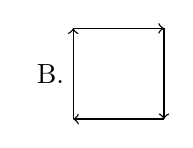
\begin{tikzpicture}[scale=0.72,line width=0.5pt]
\draw[->] (0,0)--(0,1.6);
\draw[->] (0,1.6)--(1.6,1.6);
\draw[->] (1.6,1.6)--(1.6,0);
\draw[->] (1.6,0)--(0,0);
\node at (-0.4,0.8) {B.};
\end{tikzpicture}
&
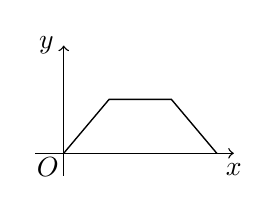
\begin{tikzpicture}[scale=0.72,line width=0.5pt]
\draw[->] (-0.5,0)--(3,0) node[below]{$x$};
\draw[->] (0,-0.4)--(0,1.9) node[left]{$y$};
\draw (0,0)--(0.8,0.95)--(1.9,0.95)--(2.7,0);
\node at (-0.28,-0.25) {$O$};
\end{tikzpicture}
\\
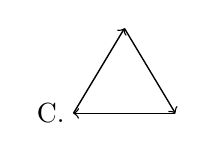
\begin{tikzpicture}[scale=0.72,line width=0.5pt]
\draw[->] (0,0)--(0.9,1.5);
\draw[->] (0.9,1.5)--(1.8,0);
\draw[->] (1.8,0)--(0,0);
\node at (-0.4,0) {C.};
\end{tikzpicture}
&
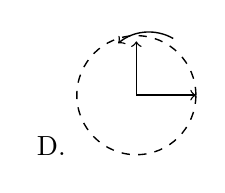
\begin{tikzpicture}[scale=0.72,line width=0.5pt]
\draw[dashed] (1.1,0.9) circle (1.05);
\draw[->] (1.1,0.9)--(2.15,0.9);
\draw[->] (1.1,0.9)--(1.1,1.85);
\draw[->] (1.75,1.9) arc (60:130:0.85);
\node at (-0.4,0) {D.};
\end{tikzpicture}
&
\end{tabular}
\end{center}

\ifanswer
\solbegin
\step{开始离家越来越远，中间离家距离不变，后来离家距离越来越近,}
\step{因此路线 $D$ 符合题意，故选 $D$.}
\solend
\fi

\item 若关于 $x$ 的方程 $ax^2+bx+c=0$（$a>0$）的两个实数根 $x_1$，$x_2$，集合
$S=\{x\mid x>x_1\}$，$T=\{x\mid x>x_2\}$，$P=\{x\mid x<x_1\}$，$Q=\{x\mid x<x_2\}$，则关于 $x$ 的不等式
$ax^2+bx+c>0$ 的解集为\mbox{（\quad）}

\keepwithprev
A. $(S\cap T)\cup(P\cap Q)$\qquad\qquad B. $(S\cap T)\cap(P\cap Q)$

C. $(S\cup T)\cup(P\cup Q)$\qquad\qquad D. $(S\cup T)\cap(P\cup Q)$

\ifanswer
\solbegin
\step{不妨设 $x_1<x_2$，则 $ax^2+bx+c>0$（$a>0$）的解集为 $\{x\mid x<x_1$ 或 $x>x_2\}$,}
\step{$S\cup T=\{x\mid x>x_1\}$，$P\cup Q=\{x\mid x<x_2\}$，$S\cap T=\{x\mid x>x_2\}$,}
\step{$P\cap Q=\{x\mid x<x_1\}$，所以 $(S\cap T)\cup(P\cap Q)=\{x\mid x<x_1$ 或 $x>x_2\}$. 故选 $A$.}
\solend
\fi

\item 已知存在函数 $y=f(x)$ 和 $y=g(x)$ 使得函数 $y=f(g(x))$ 的定义域为 $\R$，且表达式为
$f(g(x))=x^2$，则 $y=g(x)$ 的表达式不可能是\mbox{（\quad）}

\keepwithprev
A. $x^2-3\lvert x\rvert$\qquad B. $x^2+\sqrt{\lvert x\rvert}$\qquad C. $2x-1$\qquad D. $\lvert x\rvert$

\ifanswer
\solbegin
\step{对于选项 A，当 $g(x)=x^2-3\lvert x\rvert$ 时，$g(1)=g(2)=-2$.}
\step{由 $f(g(x))=x^2$ 得 $f(-2)=f(g(1))=1^2=1$，$f(-2)=f(g(2))=2^2=4$，% 原卷两处均作 f(-2)，照录
}
\step{与函数的定义矛盾，所以选项 A 不可能.}
\step{对于选项 B，当 $g(x)=x^2+\sqrt{\lvert x\rvert}$ 时,}
\step{令 $t=x^2+\sqrt{\lvert x\rvert}$，$s=\lvert x\rvert$，$h(s)=s^2+\sqrt s\ (s\geqslant0)$.}
\step{因为函数 $y=s^2$ 在区间 $[0,+\infty)$ 上严格增，函数 $y=\sqrt s$ 在区间 $[0,+\infty)$ 上严格增.}
\step{所以函数 $h(s)=s^2+\sqrt s\ (s\geqslant0)$ 在区间 $[0,+\infty)$ 上严格增.}
\step{故 $s=h^{-1}(t)$，即 $\lvert x\rvert=h^{-1}(t)$，因为 $f(g(x))=x^2=\lvert x\rvert^2$，所以 $f(t)=(h^{-1}(t))^2$,}
\step{即 $f(x)=(h^{-1}(x))^2$，此时 $y=f(g(x))$ 的定义域为 $\R$，故选项 B 可能.}
\step{对于选项 C，当 $g(x)=2x-1$ 时，由 $f(g(x))=x^2$ 得 $f(g(x))=f(2x-1)=x^2$,}
\step{则 $f(x)=\left(\dfrac{x+1}2\right)^2$，此时 $y=f(g(x))$ 的定义域为 $\R$，故选项 C 可能.}
\step{对于选项 D，当 $g(x)=\lvert x\rvert$ 时，由 $f(g(x))=x^2$ 得 $f(g(x))=f(\lvert x\rvert)=x^2$,}
\step{则 $f(x)=x^2\ (x\geqslant0)$，此时 $y=f(g(x))$ 的定义域为 $\R$，故选项 D 可能.}
\step{故选 $A$.}
\solend
\fi

\end{enumerate}

\bigsec{三、解答题}

\begin{enumerate}
\setcounter{enumi}{16}

\item 已知常数 $a\in\R$，集合 $A=\left\{x\,\middle|\,\dfrac{2x+11}{x+2}\geqslant3\right\}$，集合 $B=\{x\mid x^2+2ax-3a^2<0\}$.

（1）若 $a=2$，求 $A\cap B$；

（2）若 $A\cup B=A$，求实数 $a$ 的取值范围.

\ifanswer
\solbegin
\step{（1）$\dfrac{2x+11}{x+2}\geqslant3\Leftrightarrow\dfrac{-x+5}{x+2}\geqslant0\Leftrightarrow\dfrac{x-5}{x+2}\leqslant0\Leftrightarrow
\begin{cases}x+2\neq0\\(x-5)(x+2)\leqslant0\end{cases}$}
\step{$\Leftrightarrow-2<x\leqslant5$，$A=(-2,5]$,}
\step{当 $a=2$ 时，$B=\{x\mid x^2+4x-12<0\}=\{x\mid(x-2)(x+6)<0\}=(-6,2)$,}
\step{$A\cap B=(-2,2)$；}
\step{（2）由 $A\cup B=A$ 得 $B\subseteq A$,}
\step{当 $a=0$ 时，$B=\{x\mid x^2<0\}=\varnothing$，满足题意,}
\step{$x^2+2ax-3a^2=0$ 的两根分别是 $a$ 和 $-3a$,}
\step{当 $a>0$ 时，$B=(-3a,a)$，由题意得 $-2\leqslant-3a<a\leqslant5$，解得 $0<a\leqslant\dfrac23$,}
\step{当 $a<0$ 时，$B=(a,-3a)$，由题意得 $-2\leqslant a<-3a\leqslant5$，解得 $-\dfrac53\leqslant a<0$,}
\step{综上，$-\dfrac53\leqslant a\leqslant\dfrac23$.}
\solend
\fi

\item 某奶茶店今年年初花费 16 万元购买了一台制作冰淇淋的设备，经估算，该设备每年可
为该奶茶店提供 12 万元的总收入. 已知使用 $x$ 年（$x$ 为正整数）所需的各种维护费用总计为
$x^2+2x$ 万元（今年为第一年）.

（1）试问：该奶茶店第几年开始盈利（总收入超过总支出）？

（2）该奶茶店在若干年后要卖出该冰淇淋设备，有以下两种方案：

①当盈利总额达到最大值时，以 1 万元的价格卖出该设备；

②当年均盈利达到最大值时，以 2 万元的价格卖出该设备.

试问哪一种方案较为划算？请说明理由.

\ifanswer
\solbegin
\step{（1）由题意得总收入扣除支出后的纯收入 $y=12x-(x^2+2x+16)$}
\step{$=-x^2+10x-16$，$-x^2+10x-16>0$，解得 $2<x<8$,}
\step{由 $x\in\N^*$，所以从第三年开始盈利；}
\step{（2）方案①：纯收入 $y=-x^2+10x-16=-(x-5)^2+9$,}
\step{则 5 年后盈利总额达到最大值 9 万元，}
\step{以 1 万元的价格卖出该设备，共盈利 10 万元；}
\step{方案②：年均盈利 $z=\dfrac{-x^2+10x-16}{x}=-x+10-\dfrac{16}{x}$,}
\step{由 $x\in\N^*$，$x+\dfrac{16}{x}\geqslant2\sqrt{x\cdot\dfrac{16}{x}}=8$，当且仅当 $x=\dfrac{16}{x}$，即 $x=4$ 时取等号,}
\step{$z=-x+10-\dfrac{16}{x}\leqslant-8+10=2$，当 4 年后年均盈利达到最大值 2 万元时,}
\step{以 2 万元的价格卖出该设备，共盈利 $4\times2+2=10$ 万元.}
\step{两种方案盈利总数一样，但方案②时间短，较为划算.}
\solend
\fi

\item 已知常数 $m\in\R$，$f(x)=\sqrt{\sqrt{x(4-x)}-mx}$.% 原卷题干为双层根号，其解析按单层，见文件头注

（1）证明：对任意的 $m\in\R$，$\{x\mid y=f(x)\}\neq\varnothing$；

（2）若 $[0,2]\subseteq\{x\mid y=f(x)\}$，求实数 $m$ 的取值范围；

（3）若 $\{x\mid y=f(x)\}=[0,3]$，求实数 $m$ 的值.

\ifanswer
\solbegin
\step{（1）$\{x\mid y=f(x)\}=\{x\mid\sqrt{x(4-x)}-mx\geqslant0\}$,}
\step{由 $x(4-x)\geqslant0$ 得 $0\leqslant x\leqslant4$,}
\step{当 $m\leqslant0$ 时，由于 $0\leqslant x\leqslant4$,}
\step{所以 $\sqrt{x(4-x)}-mx\geqslant0$ 对任意 $0\leqslant x\leqslant4$ 恒成立,}
\step{故此时 $\{x\mid y=f(x)\}=\{x\mid0\leqslant x\leqslant4\}$，满足 $\{x\mid y=f(x)\}\neq\varnothing$,}
\step{当 $m>0$ 时，由于 $0\leqslant x\leqslant4$，所以 $mx\geqslant0$，所以 $x(4-x)\geqslant m^2x^2$,}
\step{得 $0\leqslant x\leqslant\dfrac4{1+m^2}$，故此时 $\{x\mid y=f(x)\}=\left\{x\,\middle|\,0\leqslant x\leqslant\dfrac4{1+m^2}\right\}$,}
\step{满足 $\{x\mid y=f(x)\}\neq\varnothing$,}
\step{所以，对任意的 $m\in\R$，$\{x\mid y=f(x)\}\neq\varnothing$；}
\step{（2）由（1）得当 $m\leqslant0$ 时，$\{x\mid y=f(x)\}=\{x\mid0\leqslant x\leqslant4\}$,}
\step{显然满足 $[0,2]\subseteq\{x\mid y=f(x)\}$.}
\step{当 $m>0$ 时，$\{x\mid y=f(x)\}=\left\{x\,\middle|\,0\leqslant x\leqslant\dfrac4{1+m^2}\right\}$,}
\step{由于 $[0,2]\subseteq\{x\mid y=f(x)\}$，所以 $\dfrac4{1+m^2}\geqslant2$，故 $0<m\leqslant1$,}
\step{综上，$m\leqslant1$；}
\step{（3）由于 $\{x\mid y=f(x)\}=[0,3]$,}
\step{所以 $m>0$，$\{x\mid y=f(x)\}=\left\{x\,\middle|\,0\leqslant x\leqslant\dfrac4{1+m^2}\right\}$,}
\step{因此 $\dfrac4{1+m^2}=3$，所以 $m=\dfrac{\sqrt3}3$.}
\solend
\fi

\item 已知函数 $y=f(x)$ 的定义域为 $\R$，其图像是一段连续曲线，对任意的 $a$、$b\in\R$，恒
有 $f(a-b)+f(a+b)=5f(a)\cdot f(b)$，且 $f(0)\neq0$，$f(1)=\dfrac23$.

（1）求 $f(0)$ 和 $f(2)$ 的值；

（2）判断函数 $y=f(x)$ 的奇偶性，并证明；

（3）证明：方程 $f(x)=5$ 在区间 $(2,3)$ 上有解.

\ifanswer
\solbegin
\step{（1）对任意的 $a$、$b\in\R$，恒有 $f(a-b)+f(a+b)=5f(a)\cdot f(b)$,}
\step{且 $f(0)\neq0$，$f(1)=\dfrac23$,}
\step{当 $a=1,b=0$ 时，$f(1)+f(1)=5f(1)\cdot f(0)$，解得 $f(0)=\dfrac25$,}
\step{当 $a=b=1$ 时，$f(0)+f(2)=5f(1)\cdot f(1)$，解得 $f(2)=\dfrac{82}{45}$；}
\step{（2）函数 $y=f(x)$ 为偶函数，证明如下：}
\step{当 $a=0,b=x$ 时，$f(-x)+f(x)=5f(0)\cdot f(x)=2f(x)$,}
\step{则有 $f(-x)=f(x)$，又函数 $y=f(x)$ 的定义域为 $\R$,}
\step{所以函数 $y=f(x)$ 为偶函数.}
\step{（2）$f(2)=\dfrac{82}{45}$% 原卷 (3) 的解答开头误标（2）并重印此行，照录
}
\step{当 $a=2,b=1$ 时，$f(1)+f(3)=5f(2)\cdot f(1)$，解得 $f(3)=\dfrac{146}{27}$,}
\step{函数 $y=f(x)$ 的图像是一段连续曲线，$\dfrac{82}{45}<5<\dfrac{146}{27}$,}
\step{所以存在 $x_0\in(2,3)$，使 $f(x_0)=5$,}
\step{即方程 $f(x)=5$ 在区间 $(2,3)$ 上有解.}
\solend
\fi

\item 若函数 $y=F(x)$ 的定义域为 $D$，且对于任意的 $x_1$、$x_2\in D$，“$F(x_1)=F(x_2)$”的充要
条件是“$x_1=x_2$”，则称函数 $y=F(x)$ 为 $D$ 上的“单值函数”. 对于函数 $y=f(x)$，记
$f^{(1)}(x)=f(x)$，$f^{(2)}(x)=f(f(x))$，$f^{(3)}(x)=f(f(f(x)))$，$\cdots$，$f^{(n+1)}(x)=f(f^{(n)}(x))$，其
中 $n=1,2,3,\cdots$，并对任意的 $A\subseteq D$，记集合 $f^{(n)}(A)=\left\{f^{(n)}(x)\mid x\in A\right\}$，并规定
$f^{(n)}(\varnothing)=\varnothing$.

（1）若 $f(x)=2x+1$，函数 $y=f(x)$ 的定义域为 $\R$，求 $f^{(2)}([0,1])$ 和 $f^{(3)}([0,1])$；

（2）若函数 $y=f(x)$ 的定义域为 $D$，且存在正整数 $m$，使得对任意的 $x\in D$，$f^{(m)}(x)=x$，
求证：函数 $y=f(x)$ 为 $D$ 上的“单值函数”；

（3）设 $a\in(0,1)$，若函数 $y=f(x)$ 的定义域为 $(0,1]$，且表达式为：
\[f(x)=\begin{cases}x+(1-a),&0<x\leqslant a,\\x-a,&a<x\leqslant1\end{cases}\]
判断 $y=f(x)$ 是否为 $(0,1]$ 上的“单值函数”，并证明对任
意的区间 $I\subseteq(0,1]$，存在正整数 $k$，使得 $f^{(k)}(I)\cap I\neq\varnothing$.

\ifanswer
\solbegin
\step{（1）当 $x\in[0,1]$ 时，$2x+1\in[1,3]$，所以 $f^{(1)}([0,1])=[1,3]$,}
\step{当 $x\in[1,3]$ 时，$2x+1\in[3,7]$，所以 $f^{(2)}([0,1])=[3,7]$,}
\step{当 $x\in[3,7]$ 时，$2x+1\in[7,15]$，所以 $f^{(3)}([0,1])=[7,15]$；}
\step{（2）由已知单值函数的定义可以改写为：若函数 $y=F(x)$ 的定义域为 $D$,}
\step{且对于任意的 $x_1$、$x_2\in D$，“$F(x_1)\neq F(x_2)$”的充要条件是“$x_1\neq x_2$”,}
\step{则称函数 $y=F(x)$ 为 $D$ 上的“单值函数.}
\step{假设 $f(x)$ 不是 $D$ 上的单值函数,}
\step{则存在 $x_1,x_2\in D,x_1\neq x_2$，$f(x_1)=f(x_2)$ 成立，即 $f^{(1)}(x_1)=f^{(1)}(x_2)$,}
\step{于是 $f\left[f^{(1)}(x_1)\right]=f\left[f^{(1)}(x_2)\right]$，即 $f^{(2)}(x_1)=f^{(2)}(x_2)$,}
\step{依此类推，得 $f^{(m)}(x_1)=f^{(m)}(x_2)$,}
\step{但由题意得 $f^{(m)}(x)=x$，因此 $f^{(2)}(x_1)=x_2$，$f^{(2)}(x_2)=x_2$，而 $x_1\neq x_2$,}
\step{因此 $f^{(m)}(x_1)\neq f^{(m)}(x_2)$，这样得出了矛盾的结论，所以假设不成立,}
\step{即 $f(x)$ 是 $D$ 上的单值函数；}
\step{（3）由新定义得 $f(x)=x+(1-a)$ 是单值函数，$f(x)=x-a$ 也是单值函数,}
\step{$0<a<1$，则 $0<1-a<1$,}
\step{又 $0<x\leqslant a$ 时，$f(x)=x+(1-a)\in(1-a,1]$,}
\step{$a<x\leqslant1$ 时，$f(x)=x-a\in(0,1-a]$，又 $(0,1-a]\cap(1-a,1]=\varnothing$,}
\step{因此对任意的 $x_1,x_2\in(0,1],x_1\neq x_2\Leftrightarrow f(x_1)\neq f(x_2)$,}
\step{所以 $y=f(x)$ 是 $(0,1]$ 上的“单值函数”,}
\step{对于任意的有限的区间 $I$，记 $\lvert I\rvert$ 表示区间 $I$ 的长度,}
\step{如果一个集合 $A$ 是若干个区间的并集,}
\step{则 $\lvert A\rvert$ 等于组成它的所有区间的长度之和,}
\step{对于任意的区间 $I\subseteq(0,1]$，$x\in I$，$f(I)=\{f(x)\mid x\in T\}$,}
\step{不妨设 $I=(s,t)$，$(0<s<t\leqslant1)$，$\lvert T\rvert=t-s$,}
\step{若 $(s,t)\subseteq(0,a]$，则 $f(I)=(s+1-a,t+1-a)$，$\lvert f(T)\rvert=t-s$,}
\step{若 $(s,t)\subseteq(a,1]$，则 $f(I)=(s-a,t-a)$，$\lvert f(T)\rvert=t-s$,}
\step{若 $a\in(s,t)$，则 $f(I)=(s+1-a,1]\cup(0,t-a)$,}
\step{$\lvert f(T)\rvert=1-(s+1-a)+(t-a)-0=t-s$，所以 $\lvert f(I)\rvert=\lvert I\rvert$,}
\step{对于任意的区间 $I\subseteq(0,1]$，显然存在正整数 $n$，使得 $n\lvert I\rvert>1$,}
\step{因此在 $f^{(0)}(I),f^{(1)}(I),f^{(2)}(I),\cdots,f^{(n)}(I)$（它们的长度和大于 1）中,}
\step{必然存在正整数 $m,l\ (m>l)$，使得 $f^{(m)}(I)\cap f^{(l)}(I)\neq\varnothing$,}
\step{因此必存在 $x,y\in I$，使得 $f^{(m)}(x)=f^{(l)}(y)$,}
\step{又 $y=f(x)$ 是 $(0,1]$ 上的单值函数,}
\step{所以 $f^{(m-1)}(x)=f^{(l-1)}(y)$，$f^{(m-2)}(x)=f^{(l-2)}(y)$，$\cdots$，$f^{(m-l)}(x)=y$,}
\step{这表示 $f^{(m-l)}(I)\cap I\neq\varnothing$，取 $k=m-l$,}
\step{所以对任意的区间 $I\subseteq(0,1]$，存在正整数 $k$，使得 $f^{(k)}(I)\cap I\neq\varnothing$.}
\solend
\fi

\end{enumerate}

\end{document}
"
% 紧凑版：xelatex "\def\iscompact{1}% 高一106_复旦附中_周末作业11期中复习.tex
%   —— 高一上数学“2026-2027 年复旦附中高一上周末作业 11 期中复习”（试卷版/答案版）
% 试卷版：xelatex 高一106_复旦附中_周末作业11期中复习.tex
% 答案版：xelatex "\def\isanswer{1}% 高一106_复旦附中_周末作业11期中复习.tex
%   —— 高一上数学“2026-2027 年复旦附中高一上周末作业 11 期中复习”（试卷版/答案版）
% 试卷版：xelatex 高一106_复旦附中_周末作业11期中复习.tex
% 答案版：xelatex "\def\isanswer{1}\input{高一106_复旦附中_周末作业11期中复习.tex}"
% 紧凑版：xelatex "\def\iscompact{1}\input{高一106_复旦附中_周末作业11期中复习.tex}"
%
% 原始材料：微信公众号“魔都数学加油站”文章，作者破晓，2026-11-03 17:19 发布；
% 连载“27学年高一106”，原文标题“27学年高一106——2026-2027年上海市复旦附中高一上周末作业11期中复习”；
% 原文链接：https://mp.weixin.qq.com/s/O3N1S8hA2awUzsOnRvCI-w。
% 正文为 9 张 PNG 页（第 1—2、4—8 页 4762×6735，第 3、9 页 2560×3620），题目下印有【解析】，为讲评版。
% 题目、解析均据原图转录；卷面水印及公众号页脚未录入。
% 第 14 题的四幅路线图选项与题干右侧的 $y$-$x$ 图像按原图形状用 TikZ 重绘。
%
% 卷首标题：原卷印作“2026-2027 年复旦附中高一上周末作业 11 期中复习”（公众号标题中的“上海市”
% 卷面标题行没有，本稿照卷面），年份区间按全稿惯例排 en dash；原卷未印副标题，本稿按题目内容
% 标为“集合与常用逻辑用语、不等式、函数”（期中复习跨三章）。
%
% 与原卷的排版差异：
%   ① 原文从第 3 题起，填空题编号为 3—12、选择题为 13—16、解答题为 17—21，本稿保留原题号；
%   ② 原卷每题下直接印【解析】，本稿按全稿惯例将解析置于答案版；第 13 题原卷把答案“$A$”
%      印在题干括号内且无【解析】，本稿试卷版留空、答案版提 \ans{}；
%   ③ 原卷未印副标题，本稿按“知识模块”口径补出；
%   ④ 原卷填空横线按全稿惯例排为 \blankline[4.4em]；解答题按惯例加 \ansspace；选择题括号排
%      \mbox{（\quad）}、选项段前按惯例加 \keepwithprev；
%   ⑤ 原卷数集排粗体 $\mathbf{R}$，按全稿惯例改 \R；
%   ⑥ 第 11 题题干“集　合　X”三字原卷字距拉得很开（铅字排版的空隙），本稿按正常字距排。
%
% 原卷存疑：第 16 题解析第二行原卷作“$f(-2)=f(g(1))=1^2=1$，$f(-2)=f(g(2))=2^2=4$”
% （两个都写 $f(-2)$；按 $g(1)=g(2)=-2$，两处相等正构成矛盾，但第二处按复合应写
% $f(g(2))=f(-2)$），本稿照录。第 19 题题干 $f(x)$ 为**双层根号**
% $\sqrt{\sqrt{x(4-x)}-mx}$，而解析 (1) 首行只写单层 $\sqrt{x(4-x)}-mx\geqslant0$
% （其后推导均按单层），原卷题干与解析不一致，各照录。
% 第 20 题解析 (3) 的解答开头原卷误标“（2）”并重印 $f(2)=\dfrac{82}{45}$ 一行，照录。
%
% 行数核对：逐题数 \step/\stepm 条数，合计 132 条（Q3：2；Q4：3；Q5：3；Q6：1；Q7：3；
% Q8：5；Q9：2；Q10：2；Q11：3；Q12：2；Q13：0；Q14：2；Q15：3；Q16：14；Q17：10；
% Q18：11；Q19：17；Q20：13；Q21：36），与原卷印刷行逐题相等。第 13 题括号内印答案、
% 无解析，提 \ans{}，不计入 \step 账。
%
\documentclass[a4paper,11pt]{article}
\usepackage{common}

\begin{document}

\examtitlest[3]{2026--2027 年复旦附中高一上周末作业 11 期中复习}{集合与常用逻辑用语、不等式、函数}

\bigsec{一、填空题}

\begin{enumerate}
\setcounter{enumi}{2}

\item 若关于 $x$ 的不等式组
$\begin{cases}2x+3>0\\x+3a<0\end{cases}$
的解集非空，则满足条件的最大整数 $a=$\blankline[4.4em].

\ifanswer
\solbegin
\step{由
$\begin{cases}2x+3>0\\x+3a<0\end{cases}$
得
$\begin{cases}x>-\dfrac32\\x<-3a\end{cases}$，
要使不等式组
$\begin{cases}2x+3>0\\x+3a<0\end{cases}$
的解集非空，}
\step{须 $-3a>-\dfrac32$，即 $a<\dfrac12$，故满足条件的最大整数 $a=0$.}
\solend
\fi

\item 若关于 $x$ 的不等式 $\lvert x-366\rvert+\lvert x-500\rvert\leqslant a$ 的解集非空，则 $a$ 的取值范围是\blankline[4.4em].

\ifanswer
\solbegin
\step{$\lvert x-366\rvert+\lvert x-500\rvert\geqslant\lvert x-366-(x-500)\rvert=134$,}
\step{当且仅当 $366\leqslant x\leqslant500$ 时取等号，所以 $\lvert x-366\rvert+\lvert x-500\rvert$ 的最小值为 134,}
\step{从而 $a\geqslant134$. 故 $a$ 的取值范围是 $[134,+\infty)$.}
\solend
\fi

\item 设集合 $A=\{1,2,3,4\}$，$B=\{1,2\}$，若 $C\subseteq A$ 且 $B\cap C\neq\varnothing$，则所有满足条件的集合 $C$ 的个数为\blankline[4.4em].

\ifanswer
\solbegin
\step{按题意，集合 $C$ 是 $A$ 的子集，且与 $B$ 的交集不为空集,}
\step{集合 $A$ 的子集有 $2^4=16$ 个，其中与 $B$ 的交集为空集的子集，即 $\{3,4\}$ 的子集,}
\step{有 $2^2=4$ 个，故满足题意的集合 $C$ 的个数为 $16-4=12$.}
\solend
\fi

\item 函数 $f(x)=\lvert x^2-3x+2\rvert$ 的单调增区间为\blankline[4.4em].

\ifanswer
\solbegin
\step{观察图像得函数 $f(x)=\lvert x^2-3x+2\rvert$ 的严格增区间为 $\left(1,\dfrac32\right),(2,+\infty)$.}
\solend
\fi

\item 已知 $f(x)=\sqrt{mx^2-mx+1}$，若函数 $y=f(x)$ 的定义域为 $\R$，则实数 $m$ 的取值范围为\blankline[4.4em].

\ifanswer
\solbegin
\step{当 $m=0$ 时，$f(x)=1$ 满足题意,}
\step{当 $m>0$ 时，$\Delta=m^2-4m\leqslant0$，所以 $0<m\leqslant4$,}
\step{故实数 $m$ 的取值范围为 $[0,4]$.}
\solend
\fi

\item 已知 $T$ 是方程 $x^2+px+q=0$（$p^2-4q>0$）的解集，$A=\{1,3,5,7,9\}$，$B=\{1,4,7,10\}$ 且 $T\cap A=\varnothing$，$T\cap B=T$，则 $p+q=$\blankline[4.4em].

\ifanswer
\solbegin
\step{对方程 $x^2+px+q=0$（$p^2-4q>0$），显然有两个根，故集合 $T$ 中有两个元素；}
\step{因为 $T\cap B=T$，所以 $T$ 中的两个元素一定在集合 $B$ 中；}
\step{又因为 $T\cap A=\varnothing$，故 $T$ 中的所有元素都不在 $A$ 中；}
\step{综上，$T$ 中的元素一定是 4 和 10，由根与系数的关系得 $14=-p,40=q$,}
\step{则 $p+q=26$.}
\solend
\fi

\item 已知正实数 $a$、$b$ 满足 $a+b=a^2+b^2$，则 $\dfrac1a+\dfrac1b$ 的最小值为\blankline[4.4em].

\ifanswer
\solbegin
\step{由已知 $\dfrac1a+\dfrac1b=\dfrac{a+b}{ab}=\dfrac{a^2+b^2}{ab}=\dfrac ab+\dfrac ba\geqslant2\sqrt{\dfrac ab\cdot\dfrac ba}=2$,}
\step{当且仅当 $\dfrac ba=\dfrac ab$，即 $a=b=1$ 时取等号，故 $\dfrac1a+\dfrac1b$ 的最小值为 $1$.}
\solend
\fi

\item 已知 $a$、$b$、$c$ 为实数，且 $a^2+c^2=64$，$b^2+c^2=100$，则 $a^2+b^2$ 的取值范围是\blankline[4.4em].

\ifanswer
\solbegin
\step{由题意得
$\begin{cases}a^2=64-c^2\\b^2=100-c^2\end{cases}\Rightarrow a^2+b^2=164-2c^2$，
其中 $0\leqslant c^2\leqslant64$,}
\step{因此 $a^2+b^2$ 的取值范围是 $[36,164]$.}
\solend
\fi

\item 设 $U$ 为全集，对集合 $X$，$Y$，定义运算“$*$”，$M*N=\overline{M\cap N}$. 已知全集
$U=\{1,2,3,4,5,6,7,8\}$，集合 $X=\{1,2,3\}$，$Y=\{3,4,5\}$，$Z=\{2,4,7\}$，则
$(X*Y)*Z=$\blankline[4.4em].% 原卷“集 合 X”三字字距拉得很开，本稿按正常字距排

\ifanswer
\solbegin
\step{因为集合 $U=\{1,2,3,4,5,6,7,8\}$，$X=\{1,2,3\}$，$Y=\{3,4,5\}$，$Z=\{2,4,7\}$,}
\step{所以 $X\cap Y=\{3\}$，则 $X*Y=\overline{X\cap Y}=\{1,2,4,5,6,7,8\}$,}
\step{又 $\{1,2,4,5,6,7,8\}\cap\{2,4,7\}=\{2,4,7\}$，所以 $(X*Y)*Z=\{1,3,5,6,8\}$.}
\solend
\fi

\item 已知一个奇函数 $y=f(x)$ 与一个偶函数 $y=g(x)$ 的和为函数 $y=\sqrt{x^2-3x+6}$，则 $f(3)=$\blankline[4.4em].

\ifanswer
\solbegin
\step{记 $h(x)=\sqrt{x^2-3x+6}$，由题意得
$\begin{cases}f(3)+g(3)=h(3)=\sqrt6\\f(-3)+g(-3)=h(-3)=2\sqrt6\end{cases}$,}
\step{又 $f(-3)=-f(3)$，$g(-3)=g(3)$，解得 $f(3)=-\dfrac{\sqrt6}2$.}
\solend
\fi

\end{enumerate}

\bigsec{二、选择题}

\begin{enumerate}
\setcounter{enumi}{12}

\item 已知 $a>b$ 均为正实数，则“$c>d$”是“$a+c>b+d$”的\mbox{（\quad）}条件% 原卷把答案“A”印在题干括号内、无【解析】

\keepwithprev
A. 充分非必要\qquad\qquad B. 必要不充分

C. 充分必要\qquad\qquad\qquad D. 既非充分又非必要

\ifanswer
\ans{$A$}
\fi

\item 如图是肖老师以恒定的速率夜跑时的离家距离 $(y)$ 与跑步时间 $(x)$ 之间的函数的图像，
则肖老师跑步的路线可能是\mbox{（\quad）}

\keepwithprev
\begin{center}
\begin{tabular}{ccc}
\begin{tikzpicture}[scale=0.72,line width=0.5pt]
\draw[->] (0,0)--(1.1,1.1);
\draw[->] (1.1,1.1)--(2.7,1.1);
\draw[->] (2.7,1.1)--(3.8,0);
\node at (-0.4,0) {A.};
\end{tikzpicture}
&
\begin{tikzpicture}[scale=0.72,line width=0.5pt]
\draw[->] (0,0)--(0,1.6);
\draw[->] (0,1.6)--(1.6,1.6);
\draw[->] (1.6,1.6)--(1.6,0);
\draw[->] (1.6,0)--(0,0);
\node at (-0.4,0.8) {B.};
\end{tikzpicture}
&
\begin{tikzpicture}[scale=0.72,line width=0.5pt]
\draw[->] (-0.5,0)--(3,0) node[below]{$x$};
\draw[->] (0,-0.4)--(0,1.9) node[left]{$y$};
\draw (0,0)--(0.8,0.95)--(1.9,0.95)--(2.7,0);
\node at (-0.28,-0.25) {$O$};
\end{tikzpicture}
\\
\begin{tikzpicture}[scale=0.72,line width=0.5pt]
\draw[->] (0,0)--(0.9,1.5);
\draw[->] (0.9,1.5)--(1.8,0);
\draw[->] (1.8,0)--(0,0);
\node at (-0.4,0) {C.};
\end{tikzpicture}
&
\begin{tikzpicture}[scale=0.72,line width=0.5pt]
\draw[dashed] (1.1,0.9) circle (1.05);
\draw[->] (1.1,0.9)--(2.15,0.9);
\draw[->] (1.1,0.9)--(1.1,1.85);
\draw[->] (1.75,1.9) arc (60:130:0.85);
\node at (-0.4,0) {D.};
\end{tikzpicture}
&
\end{tabular}
\end{center}

\ifanswer
\solbegin
\step{开始离家越来越远，中间离家距离不变，后来离家距离越来越近,}
\step{因此路线 $D$ 符合题意，故选 $D$.}
\solend
\fi

\item 若关于 $x$ 的方程 $ax^2+bx+c=0$（$a>0$）的两个实数根 $x_1$，$x_2$，集合
$S=\{x\mid x>x_1\}$，$T=\{x\mid x>x_2\}$，$P=\{x\mid x<x_1\}$，$Q=\{x\mid x<x_2\}$，则关于 $x$ 的不等式
$ax^2+bx+c>0$ 的解集为\mbox{（\quad）}

\keepwithprev
A. $(S\cap T)\cup(P\cap Q)$\qquad\qquad B. $(S\cap T)\cap(P\cap Q)$

C. $(S\cup T)\cup(P\cup Q)$\qquad\qquad D. $(S\cup T)\cap(P\cup Q)$

\ifanswer
\solbegin
\step{不妨设 $x_1<x_2$，则 $ax^2+bx+c>0$（$a>0$）的解集为 $\{x\mid x<x_1$ 或 $x>x_2\}$,}
\step{$S\cup T=\{x\mid x>x_1\}$，$P\cup Q=\{x\mid x<x_2\}$，$S\cap T=\{x\mid x>x_2\}$,}
\step{$P\cap Q=\{x\mid x<x_1\}$，所以 $(S\cap T)\cup(P\cap Q)=\{x\mid x<x_1$ 或 $x>x_2\}$. 故选 $A$.}
\solend
\fi

\item 已知存在函数 $y=f(x)$ 和 $y=g(x)$ 使得函数 $y=f(g(x))$ 的定义域为 $\R$，且表达式为
$f(g(x))=x^2$，则 $y=g(x)$ 的表达式不可能是\mbox{（\quad）}

\keepwithprev
A. $x^2-3\lvert x\rvert$\qquad B. $x^2+\sqrt{\lvert x\rvert}$\qquad C. $2x-1$\qquad D. $\lvert x\rvert$

\ifanswer
\solbegin
\step{对于选项 A，当 $g(x)=x^2-3\lvert x\rvert$ 时，$g(1)=g(2)=-2$.}
\step{由 $f(g(x))=x^2$ 得 $f(-2)=f(g(1))=1^2=1$，$f(-2)=f(g(2))=2^2=4$，% 原卷两处均作 f(-2)，照录
}
\step{与函数的定义矛盾，所以选项 A 不可能.}
\step{对于选项 B，当 $g(x)=x^2+\sqrt{\lvert x\rvert}$ 时,}
\step{令 $t=x^2+\sqrt{\lvert x\rvert}$，$s=\lvert x\rvert$，$h(s)=s^2+\sqrt s\ (s\geqslant0)$.}
\step{因为函数 $y=s^2$ 在区间 $[0,+\infty)$ 上严格增，函数 $y=\sqrt s$ 在区间 $[0,+\infty)$ 上严格增.}
\step{所以函数 $h(s)=s^2+\sqrt s\ (s\geqslant0)$ 在区间 $[0,+\infty)$ 上严格增.}
\step{故 $s=h^{-1}(t)$，即 $\lvert x\rvert=h^{-1}(t)$，因为 $f(g(x))=x^2=\lvert x\rvert^2$，所以 $f(t)=(h^{-1}(t))^2$,}
\step{即 $f(x)=(h^{-1}(x))^2$，此时 $y=f(g(x))$ 的定义域为 $\R$，故选项 B 可能.}
\step{对于选项 C，当 $g(x)=2x-1$ 时，由 $f(g(x))=x^2$ 得 $f(g(x))=f(2x-1)=x^2$,}
\step{则 $f(x)=\left(\dfrac{x+1}2\right)^2$，此时 $y=f(g(x))$ 的定义域为 $\R$，故选项 C 可能.}
\step{对于选项 D，当 $g(x)=\lvert x\rvert$ 时，由 $f(g(x))=x^2$ 得 $f(g(x))=f(\lvert x\rvert)=x^2$,}
\step{则 $f(x)=x^2\ (x\geqslant0)$，此时 $y=f(g(x))$ 的定义域为 $\R$，故选项 D 可能.}
\step{故选 $A$.}
\solend
\fi

\end{enumerate}

\bigsec{三、解答题}

\begin{enumerate}
\setcounter{enumi}{16}

\item 已知常数 $a\in\R$，集合 $A=\left\{x\,\middle|\,\dfrac{2x+11}{x+2}\geqslant3\right\}$，集合 $B=\{x\mid x^2+2ax-3a^2<0\}$.

（1）若 $a=2$，求 $A\cap B$；

（2）若 $A\cup B=A$，求实数 $a$ 的取值范围.

\ifanswer
\solbegin
\step{（1）$\dfrac{2x+11}{x+2}\geqslant3\Leftrightarrow\dfrac{-x+5}{x+2}\geqslant0\Leftrightarrow\dfrac{x-5}{x+2}\leqslant0\Leftrightarrow
\begin{cases}x+2\neq0\\(x-5)(x+2)\leqslant0\end{cases}$}
\step{$\Leftrightarrow-2<x\leqslant5$，$A=(-2,5]$,}
\step{当 $a=2$ 时，$B=\{x\mid x^2+4x-12<0\}=\{x\mid(x-2)(x+6)<0\}=(-6,2)$,}
\step{$A\cap B=(-2,2)$；}
\step{（2）由 $A\cup B=A$ 得 $B\subseteq A$,}
\step{当 $a=0$ 时，$B=\{x\mid x^2<0\}=\varnothing$，满足题意,}
\step{$x^2+2ax-3a^2=0$ 的两根分别是 $a$ 和 $-3a$,}
\step{当 $a>0$ 时，$B=(-3a,a)$，由题意得 $-2\leqslant-3a<a\leqslant5$，解得 $0<a\leqslant\dfrac23$,}
\step{当 $a<0$ 时，$B=(a,-3a)$，由题意得 $-2\leqslant a<-3a\leqslant5$，解得 $-\dfrac53\leqslant a<0$,}
\step{综上，$-\dfrac53\leqslant a\leqslant\dfrac23$.}
\solend
\fi

\item 某奶茶店今年年初花费 16 万元购买了一台制作冰淇淋的设备，经估算，该设备每年可
为该奶茶店提供 12 万元的总收入. 已知使用 $x$ 年（$x$ 为正整数）所需的各种维护费用总计为
$x^2+2x$ 万元（今年为第一年）.

（1）试问：该奶茶店第几年开始盈利（总收入超过总支出）？

（2）该奶茶店在若干年后要卖出该冰淇淋设备，有以下两种方案：

①当盈利总额达到最大值时，以 1 万元的价格卖出该设备；

②当年均盈利达到最大值时，以 2 万元的价格卖出该设备.

试问哪一种方案较为划算？请说明理由.

\ifanswer
\solbegin
\step{（1）由题意得总收入扣除支出后的纯收入 $y=12x-(x^2+2x+16)$}
\step{$=-x^2+10x-16$，$-x^2+10x-16>0$，解得 $2<x<8$,}
\step{由 $x\in\N^*$，所以从第三年开始盈利；}
\step{（2）方案①：纯收入 $y=-x^2+10x-16=-(x-5)^2+9$,}
\step{则 5 年后盈利总额达到最大值 9 万元，}
\step{以 1 万元的价格卖出该设备，共盈利 10 万元；}
\step{方案②：年均盈利 $z=\dfrac{-x^2+10x-16}{x}=-x+10-\dfrac{16}{x}$,}
\step{由 $x\in\N^*$，$x+\dfrac{16}{x}\geqslant2\sqrt{x\cdot\dfrac{16}{x}}=8$，当且仅当 $x=\dfrac{16}{x}$，即 $x=4$ 时取等号,}
\step{$z=-x+10-\dfrac{16}{x}\leqslant-8+10=2$，当 4 年后年均盈利达到最大值 2 万元时,}
\step{以 2 万元的价格卖出该设备，共盈利 $4\times2+2=10$ 万元.}
\step{两种方案盈利总数一样，但方案②时间短，较为划算.}
\solend
\fi

\item 已知常数 $m\in\R$，$f(x)=\sqrt{\sqrt{x(4-x)}-mx}$.% 原卷题干为双层根号，其解析按单层，见文件头注

（1）证明：对任意的 $m\in\R$，$\{x\mid y=f(x)\}\neq\varnothing$；

（2）若 $[0,2]\subseteq\{x\mid y=f(x)\}$，求实数 $m$ 的取值范围；

（3）若 $\{x\mid y=f(x)\}=[0,3]$，求实数 $m$ 的值.

\ifanswer
\solbegin
\step{（1）$\{x\mid y=f(x)\}=\{x\mid\sqrt{x(4-x)}-mx\geqslant0\}$,}
\step{由 $x(4-x)\geqslant0$ 得 $0\leqslant x\leqslant4$,}
\step{当 $m\leqslant0$ 时，由于 $0\leqslant x\leqslant4$,}
\step{所以 $\sqrt{x(4-x)}-mx\geqslant0$ 对任意 $0\leqslant x\leqslant4$ 恒成立,}
\step{故此时 $\{x\mid y=f(x)\}=\{x\mid0\leqslant x\leqslant4\}$，满足 $\{x\mid y=f(x)\}\neq\varnothing$,}
\step{当 $m>0$ 时，由于 $0\leqslant x\leqslant4$，所以 $mx\geqslant0$，所以 $x(4-x)\geqslant m^2x^2$,}
\step{得 $0\leqslant x\leqslant\dfrac4{1+m^2}$，故此时 $\{x\mid y=f(x)\}=\left\{x\,\middle|\,0\leqslant x\leqslant\dfrac4{1+m^2}\right\}$,}
\step{满足 $\{x\mid y=f(x)\}\neq\varnothing$,}
\step{所以，对任意的 $m\in\R$，$\{x\mid y=f(x)\}\neq\varnothing$；}
\step{（2）由（1）得当 $m\leqslant0$ 时，$\{x\mid y=f(x)\}=\{x\mid0\leqslant x\leqslant4\}$,}
\step{显然满足 $[0,2]\subseteq\{x\mid y=f(x)\}$.}
\step{当 $m>0$ 时，$\{x\mid y=f(x)\}=\left\{x\,\middle|\,0\leqslant x\leqslant\dfrac4{1+m^2}\right\}$,}
\step{由于 $[0,2]\subseteq\{x\mid y=f(x)\}$，所以 $\dfrac4{1+m^2}\geqslant2$，故 $0<m\leqslant1$,}
\step{综上，$m\leqslant1$；}
\step{（3）由于 $\{x\mid y=f(x)\}=[0,3]$,}
\step{所以 $m>0$，$\{x\mid y=f(x)\}=\left\{x\,\middle|\,0\leqslant x\leqslant\dfrac4{1+m^2}\right\}$,}
\step{因此 $\dfrac4{1+m^2}=3$，所以 $m=\dfrac{\sqrt3}3$.}
\solend
\fi

\item 已知函数 $y=f(x)$ 的定义域为 $\R$，其图像是一段连续曲线，对任意的 $a$、$b\in\R$，恒
有 $f(a-b)+f(a+b)=5f(a)\cdot f(b)$，且 $f(0)\neq0$，$f(1)=\dfrac23$.

（1）求 $f(0)$ 和 $f(2)$ 的值；

（2）判断函数 $y=f(x)$ 的奇偶性，并证明；

（3）证明：方程 $f(x)=5$ 在区间 $(2,3)$ 上有解.

\ifanswer
\solbegin
\step{（1）对任意的 $a$、$b\in\R$，恒有 $f(a-b)+f(a+b)=5f(a)\cdot f(b)$,}
\step{且 $f(0)\neq0$，$f(1)=\dfrac23$,}
\step{当 $a=1,b=0$ 时，$f(1)+f(1)=5f(1)\cdot f(0)$，解得 $f(0)=\dfrac25$,}
\step{当 $a=b=1$ 时，$f(0)+f(2)=5f(1)\cdot f(1)$，解得 $f(2)=\dfrac{82}{45}$；}
\step{（2）函数 $y=f(x)$ 为偶函数，证明如下：}
\step{当 $a=0,b=x$ 时，$f(-x)+f(x)=5f(0)\cdot f(x)=2f(x)$,}
\step{则有 $f(-x)=f(x)$，又函数 $y=f(x)$ 的定义域为 $\R$,}
\step{所以函数 $y=f(x)$ 为偶函数.}
\step{（2）$f(2)=\dfrac{82}{45}$% 原卷 (3) 的解答开头误标（2）并重印此行，照录
}
\step{当 $a=2,b=1$ 时，$f(1)+f(3)=5f(2)\cdot f(1)$，解得 $f(3)=\dfrac{146}{27}$,}
\step{函数 $y=f(x)$ 的图像是一段连续曲线，$\dfrac{82}{45}<5<\dfrac{146}{27}$,}
\step{所以存在 $x_0\in(2,3)$，使 $f(x_0)=5$,}
\step{即方程 $f(x)=5$ 在区间 $(2,3)$ 上有解.}
\solend
\fi

\item 若函数 $y=F(x)$ 的定义域为 $D$，且对于任意的 $x_1$、$x_2\in D$，“$F(x_1)=F(x_2)$”的充要
条件是“$x_1=x_2$”，则称函数 $y=F(x)$ 为 $D$ 上的“单值函数”. 对于函数 $y=f(x)$，记
$f^{(1)}(x)=f(x)$，$f^{(2)}(x)=f(f(x))$，$f^{(3)}(x)=f(f(f(x)))$，$\cdots$，$f^{(n+1)}(x)=f(f^{(n)}(x))$，其
中 $n=1,2,3,\cdots$，并对任意的 $A\subseteq D$，记集合 $f^{(n)}(A)=\left\{f^{(n)}(x)\mid x\in A\right\}$，并规定
$f^{(n)}(\varnothing)=\varnothing$.

（1）若 $f(x)=2x+1$，函数 $y=f(x)$ 的定义域为 $\R$，求 $f^{(2)}([0,1])$ 和 $f^{(3)}([0,1])$；

（2）若函数 $y=f(x)$ 的定义域为 $D$，且存在正整数 $m$，使得对任意的 $x\in D$，$f^{(m)}(x)=x$，
求证：函数 $y=f(x)$ 为 $D$ 上的“单值函数”；

（3）设 $a\in(0,1)$，若函数 $y=f(x)$ 的定义域为 $(0,1]$，且表达式为：
\[f(x)=\begin{cases}x+(1-a),&0<x\leqslant a,\\x-a,&a<x\leqslant1\end{cases}\]
判断 $y=f(x)$ 是否为 $(0,1]$ 上的“单值函数”，并证明对任
意的区间 $I\subseteq(0,1]$，存在正整数 $k$，使得 $f^{(k)}(I)\cap I\neq\varnothing$.

\ifanswer
\solbegin
\step{（1）当 $x\in[0,1]$ 时，$2x+1\in[1,3]$，所以 $f^{(1)}([0,1])=[1,3]$,}
\step{当 $x\in[1,3]$ 时，$2x+1\in[3,7]$，所以 $f^{(2)}([0,1])=[3,7]$,}
\step{当 $x\in[3,7]$ 时，$2x+1\in[7,15]$，所以 $f^{(3)}([0,1])=[7,15]$；}
\step{（2）由已知单值函数的定义可以改写为：若函数 $y=F(x)$ 的定义域为 $D$,}
\step{且对于任意的 $x_1$、$x_2\in D$，“$F(x_1)\neq F(x_2)$”的充要条件是“$x_1\neq x_2$”,}
\step{则称函数 $y=F(x)$ 为 $D$ 上的“单值函数.}
\step{假设 $f(x)$ 不是 $D$ 上的单值函数,}
\step{则存在 $x_1,x_2\in D,x_1\neq x_2$，$f(x_1)=f(x_2)$ 成立，即 $f^{(1)}(x_1)=f^{(1)}(x_2)$,}
\step{于是 $f\left[f^{(1)}(x_1)\right]=f\left[f^{(1)}(x_2)\right]$，即 $f^{(2)}(x_1)=f^{(2)}(x_2)$,}
\step{依此类推，得 $f^{(m)}(x_1)=f^{(m)}(x_2)$,}
\step{但由题意得 $f^{(m)}(x)=x$，因此 $f^{(2)}(x_1)=x_2$，$f^{(2)}(x_2)=x_2$，而 $x_1\neq x_2$,}
\step{因此 $f^{(m)}(x_1)\neq f^{(m)}(x_2)$，这样得出了矛盾的结论，所以假设不成立,}
\step{即 $f(x)$ 是 $D$ 上的单值函数；}
\step{（3）由新定义得 $f(x)=x+(1-a)$ 是单值函数，$f(x)=x-a$ 也是单值函数,}
\step{$0<a<1$，则 $0<1-a<1$,}
\step{又 $0<x\leqslant a$ 时，$f(x)=x+(1-a)\in(1-a,1]$,}
\step{$a<x\leqslant1$ 时，$f(x)=x-a\in(0,1-a]$，又 $(0,1-a]\cap(1-a,1]=\varnothing$,}
\step{因此对任意的 $x_1,x_2\in(0,1],x_1\neq x_2\Leftrightarrow f(x_1)\neq f(x_2)$,}
\step{所以 $y=f(x)$ 是 $(0,1]$ 上的“单值函数”,}
\step{对于任意的有限的区间 $I$，记 $\lvert I\rvert$ 表示区间 $I$ 的长度,}
\step{如果一个集合 $A$ 是若干个区间的并集,}
\step{则 $\lvert A\rvert$ 等于组成它的所有区间的长度之和,}
\step{对于任意的区间 $I\subseteq(0,1]$，$x\in I$，$f(I)=\{f(x)\mid x\in T\}$,}
\step{不妨设 $I=(s,t)$，$(0<s<t\leqslant1)$，$\lvert T\rvert=t-s$,}
\step{若 $(s,t)\subseteq(0,a]$，则 $f(I)=(s+1-a,t+1-a)$，$\lvert f(T)\rvert=t-s$,}
\step{若 $(s,t)\subseteq(a,1]$，则 $f(I)=(s-a,t-a)$，$\lvert f(T)\rvert=t-s$,}
\step{若 $a\in(s,t)$，则 $f(I)=(s+1-a,1]\cup(0,t-a)$,}
\step{$\lvert f(T)\rvert=1-(s+1-a)+(t-a)-0=t-s$，所以 $\lvert f(I)\rvert=\lvert I\rvert$,}
\step{对于任意的区间 $I\subseteq(0,1]$，显然存在正整数 $n$，使得 $n\lvert I\rvert>1$,}
\step{因此在 $f^{(0)}(I),f^{(1)}(I),f^{(2)}(I),\cdots,f^{(n)}(I)$（它们的长度和大于 1）中,}
\step{必然存在正整数 $m,l\ (m>l)$，使得 $f^{(m)}(I)\cap f^{(l)}(I)\neq\varnothing$,}
\step{因此必存在 $x,y\in I$，使得 $f^{(m)}(x)=f^{(l)}(y)$,}
\step{又 $y=f(x)$ 是 $(0,1]$ 上的单值函数,}
\step{所以 $f^{(m-1)}(x)=f^{(l-1)}(y)$，$f^{(m-2)}(x)=f^{(l-2)}(y)$，$\cdots$，$f^{(m-l)}(x)=y$,}
\step{这表示 $f^{(m-l)}(I)\cap I\neq\varnothing$，取 $k=m-l$,}
\step{所以对任意的区间 $I\subseteq(0,1]$，存在正整数 $k$，使得 $f^{(k)}(I)\cap I\neq\varnothing$.}
\solend
\fi

\end{enumerate}

\end{document}
"
% 紧凑版：xelatex "\def\iscompact{1}% 高一106_复旦附中_周末作业11期中复习.tex
%   —— 高一上数学“2026-2027 年复旦附中高一上周末作业 11 期中复习”（试卷版/答案版）
% 试卷版：xelatex 高一106_复旦附中_周末作业11期中复习.tex
% 答案版：xelatex "\def\isanswer{1}\input{高一106_复旦附中_周末作业11期中复习.tex}"
% 紧凑版：xelatex "\def\iscompact{1}\input{高一106_复旦附中_周末作业11期中复习.tex}"
%
% 原始材料：微信公众号“魔都数学加油站”文章，作者破晓，2026-11-03 17:19 发布；
% 连载“27学年高一106”，原文标题“27学年高一106——2026-2027年上海市复旦附中高一上周末作业11期中复习”；
% 原文链接：https://mp.weixin.qq.com/s/O3N1S8hA2awUzsOnRvCI-w。
% 正文为 9 张 PNG 页（第 1—2、4—8 页 4762×6735，第 3、9 页 2560×3620），题目下印有【解析】，为讲评版。
% 题目、解析均据原图转录；卷面水印及公众号页脚未录入。
% 第 14 题的四幅路线图选项与题干右侧的 $y$-$x$ 图像按原图形状用 TikZ 重绘。
%
% 卷首标题：原卷印作“2026-2027 年复旦附中高一上周末作业 11 期中复习”（公众号标题中的“上海市”
% 卷面标题行没有，本稿照卷面），年份区间按全稿惯例排 en dash；原卷未印副标题，本稿按题目内容
% 标为“集合与常用逻辑用语、不等式、函数”（期中复习跨三章）。
%
% 与原卷的排版差异：
%   ① 原文从第 3 题起，填空题编号为 3—12、选择题为 13—16、解答题为 17—21，本稿保留原题号；
%   ② 原卷每题下直接印【解析】，本稿按全稿惯例将解析置于答案版；第 13 题原卷把答案“$A$”
%      印在题干括号内且无【解析】，本稿试卷版留空、答案版提 \ans{}；
%   ③ 原卷未印副标题，本稿按“知识模块”口径补出；
%   ④ 原卷填空横线按全稿惯例排为 \blankline[4.4em]；解答题按惯例加 \ansspace；选择题括号排
%      \mbox{（\quad）}、选项段前按惯例加 \keepwithprev；
%   ⑤ 原卷数集排粗体 $\mathbf{R}$，按全稿惯例改 \R；
%   ⑥ 第 11 题题干“集　合　X”三字原卷字距拉得很开（铅字排版的空隙），本稿按正常字距排。
%
% 原卷存疑：第 16 题解析第二行原卷作“$f(-2)=f(g(1))=1^2=1$，$f(-2)=f(g(2))=2^2=4$”
% （两个都写 $f(-2)$；按 $g(1)=g(2)=-2$，两处相等正构成矛盾，但第二处按复合应写
% $f(g(2))=f(-2)$），本稿照录。第 19 题题干 $f(x)$ 为**双层根号**
% $\sqrt{\sqrt{x(4-x)}-mx}$，而解析 (1) 首行只写单层 $\sqrt{x(4-x)}-mx\geqslant0$
% （其后推导均按单层），原卷题干与解析不一致，各照录。
% 第 20 题解析 (3) 的解答开头原卷误标“（2）”并重印 $f(2)=\dfrac{82}{45}$ 一行，照录。
%
% 行数核对：逐题数 \step/\stepm 条数，合计 132 条（Q3：2；Q4：3；Q5：3；Q6：1；Q7：3；
% Q8：5；Q9：2；Q10：2；Q11：3；Q12：2；Q13：0；Q14：2；Q15：3；Q16：14；Q17：10；
% Q18：11；Q19：17；Q20：13；Q21：36），与原卷印刷行逐题相等。第 13 题括号内印答案、
% 无解析，提 \ans{}，不计入 \step 账。
%
\documentclass[a4paper,11pt]{article}
\usepackage{common}

\begin{document}

\examtitlest[3]{2026--2027 年复旦附中高一上周末作业 11 期中复习}{集合与常用逻辑用语、不等式、函数}

\bigsec{一、填空题}

\begin{enumerate}
\setcounter{enumi}{2}

\item 若关于 $x$ 的不等式组
$\begin{cases}2x+3>0\\x+3a<0\end{cases}$
的解集非空，则满足条件的最大整数 $a=$\blankline[4.4em].

\ifanswer
\solbegin
\step{由
$\begin{cases}2x+3>0\\x+3a<0\end{cases}$
得
$\begin{cases}x>-\dfrac32\\x<-3a\end{cases}$，
要使不等式组
$\begin{cases}2x+3>0\\x+3a<0\end{cases}$
的解集非空，}
\step{须 $-3a>-\dfrac32$，即 $a<\dfrac12$，故满足条件的最大整数 $a=0$.}
\solend
\fi

\item 若关于 $x$ 的不等式 $\lvert x-366\rvert+\lvert x-500\rvert\leqslant a$ 的解集非空，则 $a$ 的取值范围是\blankline[4.4em].

\ifanswer
\solbegin
\step{$\lvert x-366\rvert+\lvert x-500\rvert\geqslant\lvert x-366-(x-500)\rvert=134$,}
\step{当且仅当 $366\leqslant x\leqslant500$ 时取等号，所以 $\lvert x-366\rvert+\lvert x-500\rvert$ 的最小值为 134,}
\step{从而 $a\geqslant134$. 故 $a$ 的取值范围是 $[134,+\infty)$.}
\solend
\fi

\item 设集合 $A=\{1,2,3,4\}$，$B=\{1,2\}$，若 $C\subseteq A$ 且 $B\cap C\neq\varnothing$，则所有满足条件的集合 $C$ 的个数为\blankline[4.4em].

\ifanswer
\solbegin
\step{按题意，集合 $C$ 是 $A$ 的子集，且与 $B$ 的交集不为空集,}
\step{集合 $A$ 的子集有 $2^4=16$ 个，其中与 $B$ 的交集为空集的子集，即 $\{3,4\}$ 的子集,}
\step{有 $2^2=4$ 个，故满足题意的集合 $C$ 的个数为 $16-4=12$.}
\solend
\fi

\item 函数 $f(x)=\lvert x^2-3x+2\rvert$ 的单调增区间为\blankline[4.4em].

\ifanswer
\solbegin
\step{观察图像得函数 $f(x)=\lvert x^2-3x+2\rvert$ 的严格增区间为 $\left(1,\dfrac32\right),(2,+\infty)$.}
\solend
\fi

\item 已知 $f(x)=\sqrt{mx^2-mx+1}$，若函数 $y=f(x)$ 的定义域为 $\R$，则实数 $m$ 的取值范围为\blankline[4.4em].

\ifanswer
\solbegin
\step{当 $m=0$ 时，$f(x)=1$ 满足题意,}
\step{当 $m>0$ 时，$\Delta=m^2-4m\leqslant0$，所以 $0<m\leqslant4$,}
\step{故实数 $m$ 的取值范围为 $[0,4]$.}
\solend
\fi

\item 已知 $T$ 是方程 $x^2+px+q=0$（$p^2-4q>0$）的解集，$A=\{1,3,5,7,9\}$，$B=\{1,4,7,10\}$ 且 $T\cap A=\varnothing$，$T\cap B=T$，则 $p+q=$\blankline[4.4em].

\ifanswer
\solbegin
\step{对方程 $x^2+px+q=0$（$p^2-4q>0$），显然有两个根，故集合 $T$ 中有两个元素；}
\step{因为 $T\cap B=T$，所以 $T$ 中的两个元素一定在集合 $B$ 中；}
\step{又因为 $T\cap A=\varnothing$，故 $T$ 中的所有元素都不在 $A$ 中；}
\step{综上，$T$ 中的元素一定是 4 和 10，由根与系数的关系得 $14=-p,40=q$,}
\step{则 $p+q=26$.}
\solend
\fi

\item 已知正实数 $a$、$b$ 满足 $a+b=a^2+b^2$，则 $\dfrac1a+\dfrac1b$ 的最小值为\blankline[4.4em].

\ifanswer
\solbegin
\step{由已知 $\dfrac1a+\dfrac1b=\dfrac{a+b}{ab}=\dfrac{a^2+b^2}{ab}=\dfrac ab+\dfrac ba\geqslant2\sqrt{\dfrac ab\cdot\dfrac ba}=2$,}
\step{当且仅当 $\dfrac ba=\dfrac ab$，即 $a=b=1$ 时取等号，故 $\dfrac1a+\dfrac1b$ 的最小值为 $1$.}
\solend
\fi

\item 已知 $a$、$b$、$c$ 为实数，且 $a^2+c^2=64$，$b^2+c^2=100$，则 $a^2+b^2$ 的取值范围是\blankline[4.4em].

\ifanswer
\solbegin
\step{由题意得
$\begin{cases}a^2=64-c^2\\b^2=100-c^2\end{cases}\Rightarrow a^2+b^2=164-2c^2$，
其中 $0\leqslant c^2\leqslant64$,}
\step{因此 $a^2+b^2$ 的取值范围是 $[36,164]$.}
\solend
\fi

\item 设 $U$ 为全集，对集合 $X$，$Y$，定义运算“$*$”，$M*N=\overline{M\cap N}$. 已知全集
$U=\{1,2,3,4,5,6,7,8\}$，集合 $X=\{1,2,3\}$，$Y=\{3,4,5\}$，$Z=\{2,4,7\}$，则
$(X*Y)*Z=$\blankline[4.4em].% 原卷“集 合 X”三字字距拉得很开，本稿按正常字距排

\ifanswer
\solbegin
\step{因为集合 $U=\{1,2,3,4,5,6,7,8\}$，$X=\{1,2,3\}$，$Y=\{3,4,5\}$，$Z=\{2,4,7\}$,}
\step{所以 $X\cap Y=\{3\}$，则 $X*Y=\overline{X\cap Y}=\{1,2,4,5,6,7,8\}$,}
\step{又 $\{1,2,4,5,6,7,8\}\cap\{2,4,7\}=\{2,4,7\}$，所以 $(X*Y)*Z=\{1,3,5,6,8\}$.}
\solend
\fi

\item 已知一个奇函数 $y=f(x)$ 与一个偶函数 $y=g(x)$ 的和为函数 $y=\sqrt{x^2-3x+6}$，则 $f(3)=$\blankline[4.4em].

\ifanswer
\solbegin
\step{记 $h(x)=\sqrt{x^2-3x+6}$，由题意得
$\begin{cases}f(3)+g(3)=h(3)=\sqrt6\\f(-3)+g(-3)=h(-3)=2\sqrt6\end{cases}$,}
\step{又 $f(-3)=-f(3)$，$g(-3)=g(3)$，解得 $f(3)=-\dfrac{\sqrt6}2$.}
\solend
\fi

\end{enumerate}

\bigsec{二、选择题}

\begin{enumerate}
\setcounter{enumi}{12}

\item 已知 $a>b$ 均为正实数，则“$c>d$”是“$a+c>b+d$”的\mbox{（\quad）}条件% 原卷把答案“A”印在题干括号内、无【解析】

\keepwithprev
A. 充分非必要\qquad\qquad B. 必要不充分

C. 充分必要\qquad\qquad\qquad D. 既非充分又非必要

\ifanswer
\ans{$A$}
\fi

\item 如图是肖老师以恒定的速率夜跑时的离家距离 $(y)$ 与跑步时间 $(x)$ 之间的函数的图像，
则肖老师跑步的路线可能是\mbox{（\quad）}

\keepwithprev
\begin{center}
\begin{tabular}{ccc}
\begin{tikzpicture}[scale=0.72,line width=0.5pt]
\draw[->] (0,0)--(1.1,1.1);
\draw[->] (1.1,1.1)--(2.7,1.1);
\draw[->] (2.7,1.1)--(3.8,0);
\node at (-0.4,0) {A.};
\end{tikzpicture}
&
\begin{tikzpicture}[scale=0.72,line width=0.5pt]
\draw[->] (0,0)--(0,1.6);
\draw[->] (0,1.6)--(1.6,1.6);
\draw[->] (1.6,1.6)--(1.6,0);
\draw[->] (1.6,0)--(0,0);
\node at (-0.4,0.8) {B.};
\end{tikzpicture}
&
\begin{tikzpicture}[scale=0.72,line width=0.5pt]
\draw[->] (-0.5,0)--(3,0) node[below]{$x$};
\draw[->] (0,-0.4)--(0,1.9) node[left]{$y$};
\draw (0,0)--(0.8,0.95)--(1.9,0.95)--(2.7,0);
\node at (-0.28,-0.25) {$O$};
\end{tikzpicture}
\\
\begin{tikzpicture}[scale=0.72,line width=0.5pt]
\draw[->] (0,0)--(0.9,1.5);
\draw[->] (0.9,1.5)--(1.8,0);
\draw[->] (1.8,0)--(0,0);
\node at (-0.4,0) {C.};
\end{tikzpicture}
&
\begin{tikzpicture}[scale=0.72,line width=0.5pt]
\draw[dashed] (1.1,0.9) circle (1.05);
\draw[->] (1.1,0.9)--(2.15,0.9);
\draw[->] (1.1,0.9)--(1.1,1.85);
\draw[->] (1.75,1.9) arc (60:130:0.85);
\node at (-0.4,0) {D.};
\end{tikzpicture}
&
\end{tabular}
\end{center}

\ifanswer
\solbegin
\step{开始离家越来越远，中间离家距离不变，后来离家距离越来越近,}
\step{因此路线 $D$ 符合题意，故选 $D$.}
\solend
\fi

\item 若关于 $x$ 的方程 $ax^2+bx+c=0$（$a>0$）的两个实数根 $x_1$，$x_2$，集合
$S=\{x\mid x>x_1\}$，$T=\{x\mid x>x_2\}$，$P=\{x\mid x<x_1\}$，$Q=\{x\mid x<x_2\}$，则关于 $x$ 的不等式
$ax^2+bx+c>0$ 的解集为\mbox{（\quad）}

\keepwithprev
A. $(S\cap T)\cup(P\cap Q)$\qquad\qquad B. $(S\cap T)\cap(P\cap Q)$

C. $(S\cup T)\cup(P\cup Q)$\qquad\qquad D. $(S\cup T)\cap(P\cup Q)$

\ifanswer
\solbegin
\step{不妨设 $x_1<x_2$，则 $ax^2+bx+c>0$（$a>0$）的解集为 $\{x\mid x<x_1$ 或 $x>x_2\}$,}
\step{$S\cup T=\{x\mid x>x_1\}$，$P\cup Q=\{x\mid x<x_2\}$，$S\cap T=\{x\mid x>x_2\}$,}
\step{$P\cap Q=\{x\mid x<x_1\}$，所以 $(S\cap T)\cup(P\cap Q)=\{x\mid x<x_1$ 或 $x>x_2\}$. 故选 $A$.}
\solend
\fi

\item 已知存在函数 $y=f(x)$ 和 $y=g(x)$ 使得函数 $y=f(g(x))$ 的定义域为 $\R$，且表达式为
$f(g(x))=x^2$，则 $y=g(x)$ 的表达式不可能是\mbox{（\quad）}

\keepwithprev
A. $x^2-3\lvert x\rvert$\qquad B. $x^2+\sqrt{\lvert x\rvert}$\qquad C. $2x-1$\qquad D. $\lvert x\rvert$

\ifanswer
\solbegin
\step{对于选项 A，当 $g(x)=x^2-3\lvert x\rvert$ 时，$g(1)=g(2)=-2$.}
\step{由 $f(g(x))=x^2$ 得 $f(-2)=f(g(1))=1^2=1$，$f(-2)=f(g(2))=2^2=4$，% 原卷两处均作 f(-2)，照录
}
\step{与函数的定义矛盾，所以选项 A 不可能.}
\step{对于选项 B，当 $g(x)=x^2+\sqrt{\lvert x\rvert}$ 时,}
\step{令 $t=x^2+\sqrt{\lvert x\rvert}$，$s=\lvert x\rvert$，$h(s)=s^2+\sqrt s\ (s\geqslant0)$.}
\step{因为函数 $y=s^2$ 在区间 $[0,+\infty)$ 上严格增，函数 $y=\sqrt s$ 在区间 $[0,+\infty)$ 上严格增.}
\step{所以函数 $h(s)=s^2+\sqrt s\ (s\geqslant0)$ 在区间 $[0,+\infty)$ 上严格增.}
\step{故 $s=h^{-1}(t)$，即 $\lvert x\rvert=h^{-1}(t)$，因为 $f(g(x))=x^2=\lvert x\rvert^2$，所以 $f(t)=(h^{-1}(t))^2$,}
\step{即 $f(x)=(h^{-1}(x))^2$，此时 $y=f(g(x))$ 的定义域为 $\R$，故选项 B 可能.}
\step{对于选项 C，当 $g(x)=2x-1$ 时，由 $f(g(x))=x^2$ 得 $f(g(x))=f(2x-1)=x^2$,}
\step{则 $f(x)=\left(\dfrac{x+1}2\right)^2$，此时 $y=f(g(x))$ 的定义域为 $\R$，故选项 C 可能.}
\step{对于选项 D，当 $g(x)=\lvert x\rvert$ 时，由 $f(g(x))=x^2$ 得 $f(g(x))=f(\lvert x\rvert)=x^2$,}
\step{则 $f(x)=x^2\ (x\geqslant0)$，此时 $y=f(g(x))$ 的定义域为 $\R$，故选项 D 可能.}
\step{故选 $A$.}
\solend
\fi

\end{enumerate}

\bigsec{三、解答题}

\begin{enumerate}
\setcounter{enumi}{16}

\item 已知常数 $a\in\R$，集合 $A=\left\{x\,\middle|\,\dfrac{2x+11}{x+2}\geqslant3\right\}$，集合 $B=\{x\mid x^2+2ax-3a^2<0\}$.

（1）若 $a=2$，求 $A\cap B$；

（2）若 $A\cup B=A$，求实数 $a$ 的取值范围.

\ifanswer
\solbegin
\step{（1）$\dfrac{2x+11}{x+2}\geqslant3\Leftrightarrow\dfrac{-x+5}{x+2}\geqslant0\Leftrightarrow\dfrac{x-5}{x+2}\leqslant0\Leftrightarrow
\begin{cases}x+2\neq0\\(x-5)(x+2)\leqslant0\end{cases}$}
\step{$\Leftrightarrow-2<x\leqslant5$，$A=(-2,5]$,}
\step{当 $a=2$ 时，$B=\{x\mid x^2+4x-12<0\}=\{x\mid(x-2)(x+6)<0\}=(-6,2)$,}
\step{$A\cap B=(-2,2)$；}
\step{（2）由 $A\cup B=A$ 得 $B\subseteq A$,}
\step{当 $a=0$ 时，$B=\{x\mid x^2<0\}=\varnothing$，满足题意,}
\step{$x^2+2ax-3a^2=0$ 的两根分别是 $a$ 和 $-3a$,}
\step{当 $a>0$ 时，$B=(-3a,a)$，由题意得 $-2\leqslant-3a<a\leqslant5$，解得 $0<a\leqslant\dfrac23$,}
\step{当 $a<0$ 时，$B=(a,-3a)$，由题意得 $-2\leqslant a<-3a\leqslant5$，解得 $-\dfrac53\leqslant a<0$,}
\step{综上，$-\dfrac53\leqslant a\leqslant\dfrac23$.}
\solend
\fi

\item 某奶茶店今年年初花费 16 万元购买了一台制作冰淇淋的设备，经估算，该设备每年可
为该奶茶店提供 12 万元的总收入. 已知使用 $x$ 年（$x$ 为正整数）所需的各种维护费用总计为
$x^2+2x$ 万元（今年为第一年）.

（1）试问：该奶茶店第几年开始盈利（总收入超过总支出）？

（2）该奶茶店在若干年后要卖出该冰淇淋设备，有以下两种方案：

①当盈利总额达到最大值时，以 1 万元的价格卖出该设备；

②当年均盈利达到最大值时，以 2 万元的价格卖出该设备.

试问哪一种方案较为划算？请说明理由.

\ifanswer
\solbegin
\step{（1）由题意得总收入扣除支出后的纯收入 $y=12x-(x^2+2x+16)$}
\step{$=-x^2+10x-16$，$-x^2+10x-16>0$，解得 $2<x<8$,}
\step{由 $x\in\N^*$，所以从第三年开始盈利；}
\step{（2）方案①：纯收入 $y=-x^2+10x-16=-(x-5)^2+9$,}
\step{则 5 年后盈利总额达到最大值 9 万元，}
\step{以 1 万元的价格卖出该设备，共盈利 10 万元；}
\step{方案②：年均盈利 $z=\dfrac{-x^2+10x-16}{x}=-x+10-\dfrac{16}{x}$,}
\step{由 $x\in\N^*$，$x+\dfrac{16}{x}\geqslant2\sqrt{x\cdot\dfrac{16}{x}}=8$，当且仅当 $x=\dfrac{16}{x}$，即 $x=4$ 时取等号,}
\step{$z=-x+10-\dfrac{16}{x}\leqslant-8+10=2$，当 4 年后年均盈利达到最大值 2 万元时,}
\step{以 2 万元的价格卖出该设备，共盈利 $4\times2+2=10$ 万元.}
\step{两种方案盈利总数一样，但方案②时间短，较为划算.}
\solend
\fi

\item 已知常数 $m\in\R$，$f(x)=\sqrt{\sqrt{x(4-x)}-mx}$.% 原卷题干为双层根号，其解析按单层，见文件头注

（1）证明：对任意的 $m\in\R$，$\{x\mid y=f(x)\}\neq\varnothing$；

（2）若 $[0,2]\subseteq\{x\mid y=f(x)\}$，求实数 $m$ 的取值范围；

（3）若 $\{x\mid y=f(x)\}=[0,3]$，求实数 $m$ 的值.

\ifanswer
\solbegin
\step{（1）$\{x\mid y=f(x)\}=\{x\mid\sqrt{x(4-x)}-mx\geqslant0\}$,}
\step{由 $x(4-x)\geqslant0$ 得 $0\leqslant x\leqslant4$,}
\step{当 $m\leqslant0$ 时，由于 $0\leqslant x\leqslant4$,}
\step{所以 $\sqrt{x(4-x)}-mx\geqslant0$ 对任意 $0\leqslant x\leqslant4$ 恒成立,}
\step{故此时 $\{x\mid y=f(x)\}=\{x\mid0\leqslant x\leqslant4\}$，满足 $\{x\mid y=f(x)\}\neq\varnothing$,}
\step{当 $m>0$ 时，由于 $0\leqslant x\leqslant4$，所以 $mx\geqslant0$，所以 $x(4-x)\geqslant m^2x^2$,}
\step{得 $0\leqslant x\leqslant\dfrac4{1+m^2}$，故此时 $\{x\mid y=f(x)\}=\left\{x\,\middle|\,0\leqslant x\leqslant\dfrac4{1+m^2}\right\}$,}
\step{满足 $\{x\mid y=f(x)\}\neq\varnothing$,}
\step{所以，对任意的 $m\in\R$，$\{x\mid y=f(x)\}\neq\varnothing$；}
\step{（2）由（1）得当 $m\leqslant0$ 时，$\{x\mid y=f(x)\}=\{x\mid0\leqslant x\leqslant4\}$,}
\step{显然满足 $[0,2]\subseteq\{x\mid y=f(x)\}$.}
\step{当 $m>0$ 时，$\{x\mid y=f(x)\}=\left\{x\,\middle|\,0\leqslant x\leqslant\dfrac4{1+m^2}\right\}$,}
\step{由于 $[0,2]\subseteq\{x\mid y=f(x)\}$，所以 $\dfrac4{1+m^2}\geqslant2$，故 $0<m\leqslant1$,}
\step{综上，$m\leqslant1$；}
\step{（3）由于 $\{x\mid y=f(x)\}=[0,3]$,}
\step{所以 $m>0$，$\{x\mid y=f(x)\}=\left\{x\,\middle|\,0\leqslant x\leqslant\dfrac4{1+m^2}\right\}$,}
\step{因此 $\dfrac4{1+m^2}=3$，所以 $m=\dfrac{\sqrt3}3$.}
\solend
\fi

\item 已知函数 $y=f(x)$ 的定义域为 $\R$，其图像是一段连续曲线，对任意的 $a$、$b\in\R$，恒
有 $f(a-b)+f(a+b)=5f(a)\cdot f(b)$，且 $f(0)\neq0$，$f(1)=\dfrac23$.

（1）求 $f(0)$ 和 $f(2)$ 的值；

（2）判断函数 $y=f(x)$ 的奇偶性，并证明；

（3）证明：方程 $f(x)=5$ 在区间 $(2,3)$ 上有解.

\ifanswer
\solbegin
\step{（1）对任意的 $a$、$b\in\R$，恒有 $f(a-b)+f(a+b)=5f(a)\cdot f(b)$,}
\step{且 $f(0)\neq0$，$f(1)=\dfrac23$,}
\step{当 $a=1,b=0$ 时，$f(1)+f(1)=5f(1)\cdot f(0)$，解得 $f(0)=\dfrac25$,}
\step{当 $a=b=1$ 时，$f(0)+f(2)=5f(1)\cdot f(1)$，解得 $f(2)=\dfrac{82}{45}$；}
\step{（2）函数 $y=f(x)$ 为偶函数，证明如下：}
\step{当 $a=0,b=x$ 时，$f(-x)+f(x)=5f(0)\cdot f(x)=2f(x)$,}
\step{则有 $f(-x)=f(x)$，又函数 $y=f(x)$ 的定义域为 $\R$,}
\step{所以函数 $y=f(x)$ 为偶函数.}
\step{（2）$f(2)=\dfrac{82}{45}$% 原卷 (3) 的解答开头误标（2）并重印此行，照录
}
\step{当 $a=2,b=1$ 时，$f(1)+f(3)=5f(2)\cdot f(1)$，解得 $f(3)=\dfrac{146}{27}$,}
\step{函数 $y=f(x)$ 的图像是一段连续曲线，$\dfrac{82}{45}<5<\dfrac{146}{27}$,}
\step{所以存在 $x_0\in(2,3)$，使 $f(x_0)=5$,}
\step{即方程 $f(x)=5$ 在区间 $(2,3)$ 上有解.}
\solend
\fi

\item 若函数 $y=F(x)$ 的定义域为 $D$，且对于任意的 $x_1$、$x_2\in D$，“$F(x_1)=F(x_2)$”的充要
条件是“$x_1=x_2$”，则称函数 $y=F(x)$ 为 $D$ 上的“单值函数”. 对于函数 $y=f(x)$，记
$f^{(1)}(x)=f(x)$，$f^{(2)}(x)=f(f(x))$，$f^{(3)}(x)=f(f(f(x)))$，$\cdots$，$f^{(n+1)}(x)=f(f^{(n)}(x))$，其
中 $n=1,2,3,\cdots$，并对任意的 $A\subseteq D$，记集合 $f^{(n)}(A)=\left\{f^{(n)}(x)\mid x\in A\right\}$，并规定
$f^{(n)}(\varnothing)=\varnothing$.

（1）若 $f(x)=2x+1$，函数 $y=f(x)$ 的定义域为 $\R$，求 $f^{(2)}([0,1])$ 和 $f^{(3)}([0,1])$；

（2）若函数 $y=f(x)$ 的定义域为 $D$，且存在正整数 $m$，使得对任意的 $x\in D$，$f^{(m)}(x)=x$，
求证：函数 $y=f(x)$ 为 $D$ 上的“单值函数”；

（3）设 $a\in(0,1)$，若函数 $y=f(x)$ 的定义域为 $(0,1]$，且表达式为：
\[f(x)=\begin{cases}x+(1-a),&0<x\leqslant a,\\x-a,&a<x\leqslant1\end{cases}\]
判断 $y=f(x)$ 是否为 $(0,1]$ 上的“单值函数”，并证明对任
意的区间 $I\subseteq(0,1]$，存在正整数 $k$，使得 $f^{(k)}(I)\cap I\neq\varnothing$.

\ifanswer
\solbegin
\step{（1）当 $x\in[0,1]$ 时，$2x+1\in[1,3]$，所以 $f^{(1)}([0,1])=[1,3]$,}
\step{当 $x\in[1,3]$ 时，$2x+1\in[3,7]$，所以 $f^{(2)}([0,1])=[3,7]$,}
\step{当 $x\in[3,7]$ 时，$2x+1\in[7,15]$，所以 $f^{(3)}([0,1])=[7,15]$；}
\step{（2）由已知单值函数的定义可以改写为：若函数 $y=F(x)$ 的定义域为 $D$,}
\step{且对于任意的 $x_1$、$x_2\in D$，“$F(x_1)\neq F(x_2)$”的充要条件是“$x_1\neq x_2$”,}
\step{则称函数 $y=F(x)$ 为 $D$ 上的“单值函数.}
\step{假设 $f(x)$ 不是 $D$ 上的单值函数,}
\step{则存在 $x_1,x_2\in D,x_1\neq x_2$，$f(x_1)=f(x_2)$ 成立，即 $f^{(1)}(x_1)=f^{(1)}(x_2)$,}
\step{于是 $f\left[f^{(1)}(x_1)\right]=f\left[f^{(1)}(x_2)\right]$，即 $f^{(2)}(x_1)=f^{(2)}(x_2)$,}
\step{依此类推，得 $f^{(m)}(x_1)=f^{(m)}(x_2)$,}
\step{但由题意得 $f^{(m)}(x)=x$，因此 $f^{(2)}(x_1)=x_2$，$f^{(2)}(x_2)=x_2$，而 $x_1\neq x_2$,}
\step{因此 $f^{(m)}(x_1)\neq f^{(m)}(x_2)$，这样得出了矛盾的结论，所以假设不成立,}
\step{即 $f(x)$ 是 $D$ 上的单值函数；}
\step{（3）由新定义得 $f(x)=x+(1-a)$ 是单值函数，$f(x)=x-a$ 也是单值函数,}
\step{$0<a<1$，则 $0<1-a<1$,}
\step{又 $0<x\leqslant a$ 时，$f(x)=x+(1-a)\in(1-a,1]$,}
\step{$a<x\leqslant1$ 时，$f(x)=x-a\in(0,1-a]$，又 $(0,1-a]\cap(1-a,1]=\varnothing$,}
\step{因此对任意的 $x_1,x_2\in(0,1],x_1\neq x_2\Leftrightarrow f(x_1)\neq f(x_2)$,}
\step{所以 $y=f(x)$ 是 $(0,1]$ 上的“单值函数”,}
\step{对于任意的有限的区间 $I$，记 $\lvert I\rvert$ 表示区间 $I$ 的长度,}
\step{如果一个集合 $A$ 是若干个区间的并集,}
\step{则 $\lvert A\rvert$ 等于组成它的所有区间的长度之和,}
\step{对于任意的区间 $I\subseteq(0,1]$，$x\in I$，$f(I)=\{f(x)\mid x\in T\}$,}
\step{不妨设 $I=(s,t)$，$(0<s<t\leqslant1)$，$\lvert T\rvert=t-s$,}
\step{若 $(s,t)\subseteq(0,a]$，则 $f(I)=(s+1-a,t+1-a)$，$\lvert f(T)\rvert=t-s$,}
\step{若 $(s,t)\subseteq(a,1]$，则 $f(I)=(s-a,t-a)$，$\lvert f(T)\rvert=t-s$,}
\step{若 $a\in(s,t)$，则 $f(I)=(s+1-a,1]\cup(0,t-a)$,}
\step{$\lvert f(T)\rvert=1-(s+1-a)+(t-a)-0=t-s$，所以 $\lvert f(I)\rvert=\lvert I\rvert$,}
\step{对于任意的区间 $I\subseteq(0,1]$，显然存在正整数 $n$，使得 $n\lvert I\rvert>1$,}
\step{因此在 $f^{(0)}(I),f^{(1)}(I),f^{(2)}(I),\cdots,f^{(n)}(I)$（它们的长度和大于 1）中,}
\step{必然存在正整数 $m,l\ (m>l)$，使得 $f^{(m)}(I)\cap f^{(l)}(I)\neq\varnothing$,}
\step{因此必存在 $x,y\in I$，使得 $f^{(m)}(x)=f^{(l)}(y)$,}
\step{又 $y=f(x)$ 是 $(0,1]$ 上的单值函数,}
\step{所以 $f^{(m-1)}(x)=f^{(l-1)}(y)$，$f^{(m-2)}(x)=f^{(l-2)}(y)$，$\cdots$，$f^{(m-l)}(x)=y$,}
\step{这表示 $f^{(m-l)}(I)\cap I\neq\varnothing$，取 $k=m-l$,}
\step{所以对任意的区间 $I\subseteq(0,1]$，存在正整数 $k$，使得 $f^{(k)}(I)\cap I\neq\varnothing$.}
\solend
\fi

\end{enumerate}

\end{document}
"
%
% 原始材料：微信公众号“魔都数学加油站”文章，作者破晓，2026-11-03 17:19 发布；
% 连载“27学年高一106”，原文标题“27学年高一106——2026-2027年上海市复旦附中高一上周末作业11期中复习”；
% 原文链接：https://mp.weixin.qq.com/s/O3N1S8hA2awUzsOnRvCI-w。
% 正文为 9 张 PNG 页（第 1—2、4—8 页 4762×6735，第 3、9 页 2560×3620），题目下印有【解析】，为讲评版。
% 题目、解析均据原图转录；卷面水印及公众号页脚未录入。
% 第 14 题的四幅路线图选项与题干右侧的 $y$-$x$ 图像按原图形状用 TikZ 重绘。
%
% 卷首标题：原卷印作“2026-2027 年复旦附中高一上周末作业 11 期中复习”（公众号标题中的“上海市”
% 卷面标题行没有，本稿照卷面），年份区间按全稿惯例排 en dash；原卷未印副标题，本稿按题目内容
% 标为“集合与常用逻辑用语、不等式、函数”（期中复习跨三章）。
%
% 与原卷的排版差异：
%   ① 原文从第 3 题起，填空题编号为 3—12、选择题为 13—16、解答题为 17—21，本稿保留原题号；
%   ② 原卷每题下直接印【解析】，本稿按全稿惯例将解析置于答案版；第 13 题原卷把答案“$A$”
%      印在题干括号内且无【解析】，本稿试卷版留空、答案版提 \ans{}；
%   ③ 原卷未印副标题，本稿按“知识模块”口径补出；
%   ④ 原卷填空横线按全稿惯例排为 \blankline[4.4em]；解答题按惯例加 \ansspace；选择题括号排
%      \mbox{（\quad）}、选项段前按惯例加 \keepwithprev；
%   ⑤ 原卷数集排粗体 $\mathbf{R}$，按全稿惯例改 \R；
%   ⑥ 第 11 题题干“集　合　X”三字原卷字距拉得很开（铅字排版的空隙），本稿按正常字距排。
%
% 原卷存疑：第 16 题解析第二行原卷作“$f(-2)=f(g(1))=1^2=1$，$f(-2)=f(g(2))=2^2=4$”
% （两个都写 $f(-2)$；按 $g(1)=g(2)=-2$，两处相等正构成矛盾，但第二处按复合应写
% $f(g(2))=f(-2)$），本稿照录。第 19 题题干 $f(x)$ 为**双层根号**
% $\sqrt{\sqrt{x(4-x)}-mx}$，而解析 (1) 首行只写单层 $\sqrt{x(4-x)}-mx\geqslant0$
% （其后推导均按单层），原卷题干与解析不一致，各照录。
% 第 20 题解析 (3) 的解答开头原卷误标“（2）”并重印 $f(2)=\dfrac{82}{45}$ 一行，照录。
%
% 行数核对：逐题数 \step/\stepm 条数，合计 132 条（Q3：2；Q4：3；Q5：3；Q6：1；Q7：3；
% Q8：5；Q9：2；Q10：2；Q11：3；Q12：2；Q13：0；Q14：2；Q15：3；Q16：14；Q17：10；
% Q18：11；Q19：17；Q20：13；Q21：36），与原卷印刷行逐题相等。第 13 题括号内印答案、
% 无解析，提 \ans{}，不计入 \step 账。
%
\documentclass[a4paper,11pt]{article}
\usepackage{common}

\begin{document}

\examtitlest[3]{2026--2027 年复旦附中高一上周末作业 11 期中复习}{集合与常用逻辑用语、不等式、函数}

\bigsec{一、填空题}

\begin{enumerate}
\setcounter{enumi}{2}

\item 若关于 $x$ 的不等式组
$\begin{cases}2x+3>0\\x+3a<0\end{cases}$
的解集非空，则满足条件的最大整数 $a=$\blankline[4.4em].

\ifanswer
\solbegin
\step{由
$\begin{cases}2x+3>0\\x+3a<0\end{cases}$
得
$\begin{cases}x>-\dfrac32\\x<-3a\end{cases}$，
要使不等式组
$\begin{cases}2x+3>0\\x+3a<0\end{cases}$
的解集非空，}
\step{须 $-3a>-\dfrac32$，即 $a<\dfrac12$，故满足条件的最大整数 $a=0$.}
\solend
\fi

\item 若关于 $x$ 的不等式 $\lvert x-366\rvert+\lvert x-500\rvert\leqslant a$ 的解集非空，则 $a$ 的取值范围是\blankline[4.4em].

\ifanswer
\solbegin
\step{$\lvert x-366\rvert+\lvert x-500\rvert\geqslant\lvert x-366-(x-500)\rvert=134$,}
\step{当且仅当 $366\leqslant x\leqslant500$ 时取等号，所以 $\lvert x-366\rvert+\lvert x-500\rvert$ 的最小值为 134,}
\step{从而 $a\geqslant134$. 故 $a$ 的取值范围是 $[134,+\infty)$.}
\solend
\fi

\item 设集合 $A=\{1,2,3,4\}$，$B=\{1,2\}$，若 $C\subseteq A$ 且 $B\cap C\neq\varnothing$，则所有满足条件的集合 $C$ 的个数为\blankline[4.4em].

\ifanswer
\solbegin
\step{按题意，集合 $C$ 是 $A$ 的子集，且与 $B$ 的交集不为空集,}
\step{集合 $A$ 的子集有 $2^4=16$ 个，其中与 $B$ 的交集为空集的子集，即 $\{3,4\}$ 的子集,}
\step{有 $2^2=4$ 个，故满足题意的集合 $C$ 的个数为 $16-4=12$.}
\solend
\fi

\item 函数 $f(x)=\lvert x^2-3x+2\rvert$ 的单调增区间为\blankline[4.4em].

\ifanswer
\solbegin
\step{观察图像得函数 $f(x)=\lvert x^2-3x+2\rvert$ 的严格增区间为 $\left(1,\dfrac32\right),(2,+\infty)$.}
\solend
\fi

\item 已知 $f(x)=\sqrt{mx^2-mx+1}$，若函数 $y=f(x)$ 的定义域为 $\R$，则实数 $m$ 的取值范围为\blankline[4.4em].

\ifanswer
\solbegin
\step{当 $m=0$ 时，$f(x)=1$ 满足题意,}
\step{当 $m>0$ 时，$\Delta=m^2-4m\leqslant0$，所以 $0<m\leqslant4$,}
\step{故实数 $m$ 的取值范围为 $[0,4]$.}
\solend
\fi

\item 已知 $T$ 是方程 $x^2+px+q=0$（$p^2-4q>0$）的解集，$A=\{1,3,5,7,9\}$，$B=\{1,4,7,10\}$ 且 $T\cap A=\varnothing$，$T\cap B=T$，则 $p+q=$\blankline[4.4em].

\ifanswer
\solbegin
\step{对方程 $x^2+px+q=0$（$p^2-4q>0$），显然有两个根，故集合 $T$ 中有两个元素；}
\step{因为 $T\cap B=T$，所以 $T$ 中的两个元素一定在集合 $B$ 中；}
\step{又因为 $T\cap A=\varnothing$，故 $T$ 中的所有元素都不在 $A$ 中；}
\step{综上，$T$ 中的元素一定是 4 和 10，由根与系数的关系得 $14=-p,40=q$,}
\step{则 $p+q=26$.}
\solend
\fi

\item 已知正实数 $a$、$b$ 满足 $a+b=a^2+b^2$，则 $\dfrac1a+\dfrac1b$ 的最小值为\blankline[4.4em].

\ifanswer
\solbegin
\step{由已知 $\dfrac1a+\dfrac1b=\dfrac{a+b}{ab}=\dfrac{a^2+b^2}{ab}=\dfrac ab+\dfrac ba\geqslant2\sqrt{\dfrac ab\cdot\dfrac ba}=2$,}
\step{当且仅当 $\dfrac ba=\dfrac ab$，即 $a=b=1$ 时取等号，故 $\dfrac1a+\dfrac1b$ 的最小值为 $1$.}
\solend
\fi

\item 已知 $a$、$b$、$c$ 为实数，且 $a^2+c^2=64$，$b^2+c^2=100$，则 $a^2+b^2$ 的取值范围是\blankline[4.4em].

\ifanswer
\solbegin
\step{由题意得
$\begin{cases}a^2=64-c^2\\b^2=100-c^2\end{cases}\Rightarrow a^2+b^2=164-2c^2$，
其中 $0\leqslant c^2\leqslant64$,}
\step{因此 $a^2+b^2$ 的取值范围是 $[36,164]$.}
\solend
\fi

\item 设 $U$ 为全集，对集合 $X$，$Y$，定义运算“$*$”，$M*N=\overline{M\cap N}$. 已知全集
$U=\{1,2,3,4,5,6,7,8\}$，集合 $X=\{1,2,3\}$，$Y=\{3,4,5\}$，$Z=\{2,4,7\}$，则
$(X*Y)*Z=$\blankline[4.4em].% 原卷“集 合 X”三字字距拉得很开，本稿按正常字距排

\ifanswer
\solbegin
\step{因为集合 $U=\{1,2,3,4,5,6,7,8\}$，$X=\{1,2,3\}$，$Y=\{3,4,5\}$，$Z=\{2,4,7\}$,}
\step{所以 $X\cap Y=\{3\}$，则 $X*Y=\overline{X\cap Y}=\{1,2,4,5,6,7,8\}$,}
\step{又 $\{1,2,4,5,6,7,8\}\cap\{2,4,7\}=\{2,4,7\}$，所以 $(X*Y)*Z=\{1,3,5,6,8\}$.}
\solend
\fi

\item 已知一个奇函数 $y=f(x)$ 与一个偶函数 $y=g(x)$ 的和为函数 $y=\sqrt{x^2-3x+6}$，则 $f(3)=$\blankline[4.4em].

\ifanswer
\solbegin
\step{记 $h(x)=\sqrt{x^2-3x+6}$，由题意得
$\begin{cases}f(3)+g(3)=h(3)=\sqrt6\\f(-3)+g(-3)=h(-3)=2\sqrt6\end{cases}$,}
\step{又 $f(-3)=-f(3)$，$g(-3)=g(3)$，解得 $f(3)=-\dfrac{\sqrt6}2$.}
\solend
\fi

\end{enumerate}

\bigsec{二、选择题}

\begin{enumerate}
\setcounter{enumi}{12}

\item 已知 $a>b$ 均为正实数，则“$c>d$”是“$a+c>b+d$”的\mbox{（\quad）}条件% 原卷把答案“A”印在题干括号内、无【解析】

\keepwithprev
A. 充分非必要\qquad\qquad B. 必要不充分

C. 充分必要\qquad\qquad\qquad D. 既非充分又非必要

\ifanswer
\ans{$A$}
\fi

\item 如图是肖老师以恒定的速率夜跑时的离家距离 $(y)$ 与跑步时间 $(x)$ 之间的函数的图像，
则肖老师跑步的路线可能是\mbox{（\quad）}

\keepwithprev
\begin{center}
\begin{tabular}{ccc}
\begin{tikzpicture}[scale=0.72,line width=0.5pt]
\draw[->] (0,0)--(1.1,1.1);
\draw[->] (1.1,1.1)--(2.7,1.1);
\draw[->] (2.7,1.1)--(3.8,0);
\node at (-0.4,0) {A.};
\end{tikzpicture}
&
\begin{tikzpicture}[scale=0.72,line width=0.5pt]
\draw[->] (0,0)--(0,1.6);
\draw[->] (0,1.6)--(1.6,1.6);
\draw[->] (1.6,1.6)--(1.6,0);
\draw[->] (1.6,0)--(0,0);
\node at (-0.4,0.8) {B.};
\end{tikzpicture}
&
\begin{tikzpicture}[scale=0.72,line width=0.5pt]
\draw[->] (-0.5,0)--(3,0) node[below]{$x$};
\draw[->] (0,-0.4)--(0,1.9) node[left]{$y$};
\draw (0,0)--(0.8,0.95)--(1.9,0.95)--(2.7,0);
\node at (-0.28,-0.25) {$O$};
\end{tikzpicture}
\\
\begin{tikzpicture}[scale=0.72,line width=0.5pt]
\draw[->] (0,0)--(0.9,1.5);
\draw[->] (0.9,1.5)--(1.8,0);
\draw[->] (1.8,0)--(0,0);
\node at (-0.4,0) {C.};
\end{tikzpicture}
&
\begin{tikzpicture}[scale=0.72,line width=0.5pt]
\draw[dashed] (1.1,0.9) circle (1.05);
\draw[->] (1.1,0.9)--(2.15,0.9);
\draw[->] (1.1,0.9)--(1.1,1.85);
\draw[->] (1.75,1.9) arc (60:130:0.85);
\node at (-0.4,0) {D.};
\end{tikzpicture}
&
\end{tabular}
\end{center}

\ifanswer
\solbegin
\step{开始离家越来越远，中间离家距离不变，后来离家距离越来越近,}
\step{因此路线 $D$ 符合题意，故选 $D$.}
\solend
\fi

\item 若关于 $x$ 的方程 $ax^2+bx+c=0$（$a>0$）的两个实数根 $x_1$，$x_2$，集合
$S=\{x\mid x>x_1\}$，$T=\{x\mid x>x_2\}$，$P=\{x\mid x<x_1\}$，$Q=\{x\mid x<x_2\}$，则关于 $x$ 的不等式
$ax^2+bx+c>0$ 的解集为\mbox{（\quad）}

\keepwithprev
A. $(S\cap T)\cup(P\cap Q)$\qquad\qquad B. $(S\cap T)\cap(P\cap Q)$

C. $(S\cup T)\cup(P\cup Q)$\qquad\qquad D. $(S\cup T)\cap(P\cup Q)$

\ifanswer
\solbegin
\step{不妨设 $x_1<x_2$，则 $ax^2+bx+c>0$（$a>0$）的解集为 $\{x\mid x<x_1$ 或 $x>x_2\}$,}
\step{$S\cup T=\{x\mid x>x_1\}$，$P\cup Q=\{x\mid x<x_2\}$，$S\cap T=\{x\mid x>x_2\}$,}
\step{$P\cap Q=\{x\mid x<x_1\}$，所以 $(S\cap T)\cup(P\cap Q)=\{x\mid x<x_1$ 或 $x>x_2\}$. 故选 $A$.}
\solend
\fi

\item 已知存在函数 $y=f(x)$ 和 $y=g(x)$ 使得函数 $y=f(g(x))$ 的定义域为 $\R$，且表达式为
$f(g(x))=x^2$，则 $y=g(x)$ 的表达式不可能是\mbox{（\quad）}

\keepwithprev
A. $x^2-3\lvert x\rvert$\qquad B. $x^2+\sqrt{\lvert x\rvert}$\qquad C. $2x-1$\qquad D. $\lvert x\rvert$

\ifanswer
\solbegin
\step{对于选项 A，当 $g(x)=x^2-3\lvert x\rvert$ 时，$g(1)=g(2)=-2$.}
\step{由 $f(g(x))=x^2$ 得 $f(-2)=f(g(1))=1^2=1$，$f(-2)=f(g(2))=2^2=4$，% 原卷两处均作 f(-2)，照录
}
\step{与函数的定义矛盾，所以选项 A 不可能.}
\step{对于选项 B，当 $g(x)=x^2+\sqrt{\lvert x\rvert}$ 时,}
\step{令 $t=x^2+\sqrt{\lvert x\rvert}$，$s=\lvert x\rvert$，$h(s)=s^2+\sqrt s\ (s\geqslant0)$.}
\step{因为函数 $y=s^2$ 在区间 $[0,+\infty)$ 上严格增，函数 $y=\sqrt s$ 在区间 $[0,+\infty)$ 上严格增.}
\step{所以函数 $h(s)=s^2+\sqrt s\ (s\geqslant0)$ 在区间 $[0,+\infty)$ 上严格增.}
\step{故 $s=h^{-1}(t)$，即 $\lvert x\rvert=h^{-1}(t)$，因为 $f(g(x))=x^2=\lvert x\rvert^2$，所以 $f(t)=(h^{-1}(t))^2$,}
\step{即 $f(x)=(h^{-1}(x))^2$，此时 $y=f(g(x))$ 的定义域为 $\R$，故选项 B 可能.}
\step{对于选项 C，当 $g(x)=2x-1$ 时，由 $f(g(x))=x^2$ 得 $f(g(x))=f(2x-1)=x^2$,}
\step{则 $f(x)=\left(\dfrac{x+1}2\right)^2$，此时 $y=f(g(x))$ 的定义域为 $\R$，故选项 C 可能.}
\step{对于选项 D，当 $g(x)=\lvert x\rvert$ 时，由 $f(g(x))=x^2$ 得 $f(g(x))=f(\lvert x\rvert)=x^2$,}
\step{则 $f(x)=x^2\ (x\geqslant0)$，此时 $y=f(g(x))$ 的定义域为 $\R$，故选项 D 可能.}
\step{故选 $A$.}
\solend
\fi

\end{enumerate}

\bigsec{三、解答题}

\begin{enumerate}
\setcounter{enumi}{16}

\item 已知常数 $a\in\R$，集合 $A=\left\{x\,\middle|\,\dfrac{2x+11}{x+2}\geqslant3\right\}$，集合 $B=\{x\mid x^2+2ax-3a^2<0\}$.

（1）若 $a=2$，求 $A\cap B$；

（2）若 $A\cup B=A$，求实数 $a$ 的取值范围.

\ifanswer
\solbegin
\step{（1）$\dfrac{2x+11}{x+2}\geqslant3\Leftrightarrow\dfrac{-x+5}{x+2}\geqslant0\Leftrightarrow\dfrac{x-5}{x+2}\leqslant0\Leftrightarrow
\begin{cases}x+2\neq0\\(x-5)(x+2)\leqslant0\end{cases}$}
\step{$\Leftrightarrow-2<x\leqslant5$，$A=(-2,5]$,}
\step{当 $a=2$ 时，$B=\{x\mid x^2+4x-12<0\}=\{x\mid(x-2)(x+6)<0\}=(-6,2)$,}
\step{$A\cap B=(-2,2)$；}
\step{（2）由 $A\cup B=A$ 得 $B\subseteq A$,}
\step{当 $a=0$ 时，$B=\{x\mid x^2<0\}=\varnothing$，满足题意,}
\step{$x^2+2ax-3a^2=0$ 的两根分别是 $a$ 和 $-3a$,}
\step{当 $a>0$ 时，$B=(-3a,a)$，由题意得 $-2\leqslant-3a<a\leqslant5$，解得 $0<a\leqslant\dfrac23$,}
\step{当 $a<0$ 时，$B=(a,-3a)$，由题意得 $-2\leqslant a<-3a\leqslant5$，解得 $-\dfrac53\leqslant a<0$,}
\step{综上，$-\dfrac53\leqslant a\leqslant\dfrac23$.}
\solend
\fi

\item 某奶茶店今年年初花费 16 万元购买了一台制作冰淇淋的设备，经估算，该设备每年可
为该奶茶店提供 12 万元的总收入. 已知使用 $x$ 年（$x$ 为正整数）所需的各种维护费用总计为
$x^2+2x$ 万元（今年为第一年）.

（1）试问：该奶茶店第几年开始盈利（总收入超过总支出）？

（2）该奶茶店在若干年后要卖出该冰淇淋设备，有以下两种方案：

①当盈利总额达到最大值时，以 1 万元的价格卖出该设备；

②当年均盈利达到最大值时，以 2 万元的价格卖出该设备.

试问哪一种方案较为划算？请说明理由.

\ifanswer
\solbegin
\step{（1）由题意得总收入扣除支出后的纯收入 $y=12x-(x^2+2x+16)$}
\step{$=-x^2+10x-16$，$-x^2+10x-16>0$，解得 $2<x<8$,}
\step{由 $x\in\N^*$，所以从第三年开始盈利；}
\step{（2）方案①：纯收入 $y=-x^2+10x-16=-(x-5)^2+9$,}
\step{则 5 年后盈利总额达到最大值 9 万元，}
\step{以 1 万元的价格卖出该设备，共盈利 10 万元；}
\step{方案②：年均盈利 $z=\dfrac{-x^2+10x-16}{x}=-x+10-\dfrac{16}{x}$,}
\step{由 $x\in\N^*$，$x+\dfrac{16}{x}\geqslant2\sqrt{x\cdot\dfrac{16}{x}}=8$，当且仅当 $x=\dfrac{16}{x}$，即 $x=4$ 时取等号,}
\step{$z=-x+10-\dfrac{16}{x}\leqslant-8+10=2$，当 4 年后年均盈利达到最大值 2 万元时,}
\step{以 2 万元的价格卖出该设备，共盈利 $4\times2+2=10$ 万元.}
\step{两种方案盈利总数一样，但方案②时间短，较为划算.}
\solend
\fi

\item 已知常数 $m\in\R$，$f(x)=\sqrt{\sqrt{x(4-x)}-mx}$.% 原卷题干为双层根号，其解析按单层，见文件头注

（1）证明：对任意的 $m\in\R$，$\{x\mid y=f(x)\}\neq\varnothing$；

（2）若 $[0,2]\subseteq\{x\mid y=f(x)\}$，求实数 $m$ 的取值范围；

（3）若 $\{x\mid y=f(x)\}=[0,3]$，求实数 $m$ 的值.

\ifanswer
\solbegin
\step{（1）$\{x\mid y=f(x)\}=\{x\mid\sqrt{x(4-x)}-mx\geqslant0\}$,}
\step{由 $x(4-x)\geqslant0$ 得 $0\leqslant x\leqslant4$,}
\step{当 $m\leqslant0$ 时，由于 $0\leqslant x\leqslant4$,}
\step{所以 $\sqrt{x(4-x)}-mx\geqslant0$ 对任意 $0\leqslant x\leqslant4$ 恒成立,}
\step{故此时 $\{x\mid y=f(x)\}=\{x\mid0\leqslant x\leqslant4\}$，满足 $\{x\mid y=f(x)\}\neq\varnothing$,}
\step{当 $m>0$ 时，由于 $0\leqslant x\leqslant4$，所以 $mx\geqslant0$，所以 $x(4-x)\geqslant m^2x^2$,}
\step{得 $0\leqslant x\leqslant\dfrac4{1+m^2}$，故此时 $\{x\mid y=f(x)\}=\left\{x\,\middle|\,0\leqslant x\leqslant\dfrac4{1+m^2}\right\}$,}
\step{满足 $\{x\mid y=f(x)\}\neq\varnothing$,}
\step{所以，对任意的 $m\in\R$，$\{x\mid y=f(x)\}\neq\varnothing$；}
\step{（2）由（1）得当 $m\leqslant0$ 时，$\{x\mid y=f(x)\}=\{x\mid0\leqslant x\leqslant4\}$,}
\step{显然满足 $[0,2]\subseteq\{x\mid y=f(x)\}$.}
\step{当 $m>0$ 时，$\{x\mid y=f(x)\}=\left\{x\,\middle|\,0\leqslant x\leqslant\dfrac4{1+m^2}\right\}$,}
\step{由于 $[0,2]\subseteq\{x\mid y=f(x)\}$，所以 $\dfrac4{1+m^2}\geqslant2$，故 $0<m\leqslant1$,}
\step{综上，$m\leqslant1$；}
\step{（3）由于 $\{x\mid y=f(x)\}=[0,3]$,}
\step{所以 $m>0$，$\{x\mid y=f(x)\}=\left\{x\,\middle|\,0\leqslant x\leqslant\dfrac4{1+m^2}\right\}$,}
\step{因此 $\dfrac4{1+m^2}=3$，所以 $m=\dfrac{\sqrt3}3$.}
\solend
\fi

\item 已知函数 $y=f(x)$ 的定义域为 $\R$，其图像是一段连续曲线，对任意的 $a$、$b\in\R$，恒
有 $f(a-b)+f(a+b)=5f(a)\cdot f(b)$，且 $f(0)\neq0$，$f(1)=\dfrac23$.

（1）求 $f(0)$ 和 $f(2)$ 的值；

（2）判断函数 $y=f(x)$ 的奇偶性，并证明；

（3）证明：方程 $f(x)=5$ 在区间 $(2,3)$ 上有解.

\ifanswer
\solbegin
\step{（1）对任意的 $a$、$b\in\R$，恒有 $f(a-b)+f(a+b)=5f(a)\cdot f(b)$,}
\step{且 $f(0)\neq0$，$f(1)=\dfrac23$,}
\step{当 $a=1,b=0$ 时，$f(1)+f(1)=5f(1)\cdot f(0)$，解得 $f(0)=\dfrac25$,}
\step{当 $a=b=1$ 时，$f(0)+f(2)=5f(1)\cdot f(1)$，解得 $f(2)=\dfrac{82}{45}$；}
\step{（2）函数 $y=f(x)$ 为偶函数，证明如下：}
\step{当 $a=0,b=x$ 时，$f(-x)+f(x)=5f(0)\cdot f(x)=2f(x)$,}
\step{则有 $f(-x)=f(x)$，又函数 $y=f(x)$ 的定义域为 $\R$,}
\step{所以函数 $y=f(x)$ 为偶函数.}
\step{（2）$f(2)=\dfrac{82}{45}$% 原卷 (3) 的解答开头误标（2）并重印此行，照录
}
\step{当 $a=2,b=1$ 时，$f(1)+f(3)=5f(2)\cdot f(1)$，解得 $f(3)=\dfrac{146}{27}$,}
\step{函数 $y=f(x)$ 的图像是一段连续曲线，$\dfrac{82}{45}<5<\dfrac{146}{27}$,}
\step{所以存在 $x_0\in(2,3)$，使 $f(x_0)=5$,}
\step{即方程 $f(x)=5$ 在区间 $(2,3)$ 上有解.}
\solend
\fi

\item 若函数 $y=F(x)$ 的定义域为 $D$，且对于任意的 $x_1$、$x_2\in D$，“$F(x_1)=F(x_2)$”的充要
条件是“$x_1=x_2$”，则称函数 $y=F(x)$ 为 $D$ 上的“单值函数”. 对于函数 $y=f(x)$，记
$f^{(1)}(x)=f(x)$，$f^{(2)}(x)=f(f(x))$，$f^{(3)}(x)=f(f(f(x)))$，$\cdots$，$f^{(n+1)}(x)=f(f^{(n)}(x))$，其
中 $n=1,2,3,\cdots$，并对任意的 $A\subseteq D$，记集合 $f^{(n)}(A)=\left\{f^{(n)}(x)\mid x\in A\right\}$，并规定
$f^{(n)}(\varnothing)=\varnothing$.

（1）若 $f(x)=2x+1$，函数 $y=f(x)$ 的定义域为 $\R$，求 $f^{(2)}([0,1])$ 和 $f^{(3)}([0,1])$；

（2）若函数 $y=f(x)$ 的定义域为 $D$，且存在正整数 $m$，使得对任意的 $x\in D$，$f^{(m)}(x)=x$，
求证：函数 $y=f(x)$ 为 $D$ 上的“单值函数”；

（3）设 $a\in(0,1)$，若函数 $y=f(x)$ 的定义域为 $(0,1]$，且表达式为：
\[f(x)=\begin{cases}x+(1-a),&0<x\leqslant a,\\x-a,&a<x\leqslant1\end{cases}\]
判断 $y=f(x)$ 是否为 $(0,1]$ 上的“单值函数”，并证明对任
意的区间 $I\subseteq(0,1]$，存在正整数 $k$，使得 $f^{(k)}(I)\cap I\neq\varnothing$.

\ifanswer
\solbegin
\step{（1）当 $x\in[0,1]$ 时，$2x+1\in[1,3]$，所以 $f^{(1)}([0,1])=[1,3]$,}
\step{当 $x\in[1,3]$ 时，$2x+1\in[3,7]$，所以 $f^{(2)}([0,1])=[3,7]$,}
\step{当 $x\in[3,7]$ 时，$2x+1\in[7,15]$，所以 $f^{(3)}([0,1])=[7,15]$；}
\step{（2）由已知单值函数的定义可以改写为：若函数 $y=F(x)$ 的定义域为 $D$,}
\step{且对于任意的 $x_1$、$x_2\in D$，“$F(x_1)\neq F(x_2)$”的充要条件是“$x_1\neq x_2$”,}
\step{则称函数 $y=F(x)$ 为 $D$ 上的“单值函数.}
\step{假设 $f(x)$ 不是 $D$ 上的单值函数,}
\step{则存在 $x_1,x_2\in D,x_1\neq x_2$，$f(x_1)=f(x_2)$ 成立，即 $f^{(1)}(x_1)=f^{(1)}(x_2)$,}
\step{于是 $f\left[f^{(1)}(x_1)\right]=f\left[f^{(1)}(x_2)\right]$，即 $f^{(2)}(x_1)=f^{(2)}(x_2)$,}
\step{依此类推，得 $f^{(m)}(x_1)=f^{(m)}(x_2)$,}
\step{但由题意得 $f^{(m)}(x)=x$，因此 $f^{(2)}(x_1)=x_2$，$f^{(2)}(x_2)=x_2$，而 $x_1\neq x_2$,}
\step{因此 $f^{(m)}(x_1)\neq f^{(m)}(x_2)$，这样得出了矛盾的结论，所以假设不成立,}
\step{即 $f(x)$ 是 $D$ 上的单值函数；}
\step{（3）由新定义得 $f(x)=x+(1-a)$ 是单值函数，$f(x)=x-a$ 也是单值函数,}
\step{$0<a<1$，则 $0<1-a<1$,}
\step{又 $0<x\leqslant a$ 时，$f(x)=x+(1-a)\in(1-a,1]$,}
\step{$a<x\leqslant1$ 时，$f(x)=x-a\in(0,1-a]$，又 $(0,1-a]\cap(1-a,1]=\varnothing$,}
\step{因此对任意的 $x_1,x_2\in(0,1],x_1\neq x_2\Leftrightarrow f(x_1)\neq f(x_2)$,}
\step{所以 $y=f(x)$ 是 $(0,1]$ 上的“单值函数”,}
\step{对于任意的有限的区间 $I$，记 $\lvert I\rvert$ 表示区间 $I$ 的长度,}
\step{如果一个集合 $A$ 是若干个区间的并集,}
\step{则 $\lvert A\rvert$ 等于组成它的所有区间的长度之和,}
\step{对于任意的区间 $I\subseteq(0,1]$，$x\in I$，$f(I)=\{f(x)\mid x\in T\}$,}
\step{不妨设 $I=(s,t)$，$(0<s<t\leqslant1)$，$\lvert T\rvert=t-s$,}
\step{若 $(s,t)\subseteq(0,a]$，则 $f(I)=(s+1-a,t+1-a)$，$\lvert f(T)\rvert=t-s$,}
\step{若 $(s,t)\subseteq(a,1]$，则 $f(I)=(s-a,t-a)$，$\lvert f(T)\rvert=t-s$,}
\step{若 $a\in(s,t)$，则 $f(I)=(s+1-a,1]\cup(0,t-a)$,}
\step{$\lvert f(T)\rvert=1-(s+1-a)+(t-a)-0=t-s$，所以 $\lvert f(I)\rvert=\lvert I\rvert$,}
\step{对于任意的区间 $I\subseteq(0,1]$，显然存在正整数 $n$，使得 $n\lvert I\rvert>1$,}
\step{因此在 $f^{(0)}(I),f^{(1)}(I),f^{(2)}(I),\cdots,f^{(n)}(I)$（它们的长度和大于 1）中,}
\step{必然存在正整数 $m,l\ (m>l)$，使得 $f^{(m)}(I)\cap f^{(l)}(I)\neq\varnothing$,}
\step{因此必存在 $x,y\in I$，使得 $f^{(m)}(x)=f^{(l)}(y)$,}
\step{又 $y=f(x)$ 是 $(0,1]$ 上的单值函数,}
\step{所以 $f^{(m-1)}(x)=f^{(l-1)}(y)$，$f^{(m-2)}(x)=f^{(l-2)}(y)$，$\cdots$，$f^{(m-l)}(x)=y$,}
\step{这表示 $f^{(m-l)}(I)\cap I\neq\varnothing$，取 $k=m-l$,}
\step{所以对任意的区间 $I\subseteq(0,1]$，存在正整数 $k$，使得 $f^{(k)}(I)\cap I\neq\varnothing$.}
\solend
\fi

\end{enumerate}

\end{document}
"
%
% 原始材料：微信公众号“魔都数学加油站”文章，作者破晓，2026-11-03 17:19 发布；
% 连载“27学年高一106”，原文标题“27学年高一106——2026-2027年上海市复旦附中高一上周末作业11期中复习”；
% 原文链接：https://mp.weixin.qq.com/s/O3N1S8hA2awUzsOnRvCI-w。
% 正文为 9 张 PNG 页（第 1—2、4—8 页 4762×6735，第 3、9 页 2560×3620），题目下印有【解析】，为讲评版。
% 题目、解析均据原图转录；卷面水印及公众号页脚未录入。
% 第 14 题的四幅路线图选项与题干右侧的 $y$-$x$ 图像按原图形状用 TikZ 重绘。
%
% 卷首标题：原卷印作“2026-2027 年复旦附中高一上周末作业 11 期中复习”（公众号标题中的“上海市”
% 卷面标题行没有，本稿照卷面），年份区间按全稿惯例排 en dash；原卷未印副标题，本稿按题目内容
% 标为“集合与常用逻辑用语、不等式、函数”（期中复习跨三章）。
%
% 与原卷的排版差异：
%   ① 原文从第 3 题起，填空题编号为 3—12、选择题为 13—16、解答题为 17—21，本稿保留原题号；
%   ② 原卷每题下直接印【解析】，本稿按全稿惯例将解析置于答案版；第 13 题原卷把答案“$A$”
%      印在题干括号内且无【解析】，本稿试卷版留空、答案版提 \ans{}；
%   ③ 原卷未印副标题，本稿按“知识模块”口径补出；
%   ④ 原卷填空横线按全稿惯例排为 \blankline[4.4em]；解答题按惯例加 \ansspace；选择题括号排
%      \mbox{（\quad）}、选项段前按惯例加 \keepwithprev；
%   ⑤ 原卷数集排粗体 $\mathbf{R}$，按全稿惯例改 \R；
%   ⑥ 第 11 题题干“集　合　X”三字原卷字距拉得很开（铅字排版的空隙），本稿按正常字距排。
%
% 原卷存疑：第 16 题解析第二行原卷作“$f(-2)=f(g(1))=1^2=1$，$f(-2)=f(g(2))=2^2=4$”
% （两个都写 $f(-2)$；按 $g(1)=g(2)=-2$，两处相等正构成矛盾，但第二处按复合应写
% $f(g(2))=f(-2)$），本稿照录。第 19 题题干 $f(x)$ 为**双层根号**
% $\sqrt{\sqrt{x(4-x)}-mx}$，而解析 (1) 首行只写单层 $\sqrt{x(4-x)}-mx\geqslant0$
% （其后推导均按单层），原卷题干与解析不一致，各照录。
% 第 20 题解析 (3) 的解答开头原卷误标“（2）”并重印 $f(2)=\dfrac{82}{45}$ 一行，照录。
%
% 行数核对：逐题数 \step/\stepm 条数，合计 132 条（Q3：2；Q4：3；Q5：3；Q6：1；Q7：3；
% Q8：5；Q9：2；Q10：2；Q11：3；Q12：2；Q13：0；Q14：2；Q15：3；Q16：14；Q17：10；
% Q18：11；Q19：17；Q20：13；Q21：36），与原卷印刷行逐题相等。第 13 题括号内印答案、
% 无解析，提 \ans{}，不计入 \step 账。
%
\documentclass[a4paper,11pt]{article}
\usepackage{common}

\begin{document}

\examtitlest[3]{2026--2027 年复旦附中高一上周末作业 11 期中复习}{集合与常用逻辑用语、不等式、函数}

\bigsec{一、填空题}

\begin{enumerate}
\setcounter{enumi}{2}

\item 若关于 $x$ 的不等式组
$\begin{cases}2x+3>0\\x+3a<0\end{cases}$
的解集非空，则满足条件的最大整数 $a=$\blankline[4.4em].

\ifanswer
\solbegin
\step{由
$\begin{cases}2x+3>0\\x+3a<0\end{cases}$
得
$\begin{cases}x>-\dfrac32\\x<-3a\end{cases}$，
要使不等式组
$\begin{cases}2x+3>0\\x+3a<0\end{cases}$
的解集非空，}
\step{须 $-3a>-\dfrac32$，即 $a<\dfrac12$，故满足条件的最大整数 $a=0$.}
\solend
\fi

\item 若关于 $x$ 的不等式 $\lvert x-366\rvert+\lvert x-500\rvert\leqslant a$ 的解集非空，则 $a$ 的取值范围是\blankline[4.4em].

\ifanswer
\solbegin
\step{$\lvert x-366\rvert+\lvert x-500\rvert\geqslant\lvert x-366-(x-500)\rvert=134$,}
\step{当且仅当 $366\leqslant x\leqslant500$ 时取等号，所以 $\lvert x-366\rvert+\lvert x-500\rvert$ 的最小值为 134,}
\step{从而 $a\geqslant134$. 故 $a$ 的取值范围是 $[134,+\infty)$.}
\solend
\fi

\item 设集合 $A=\{1,2,3,4\}$，$B=\{1,2\}$，若 $C\subseteq A$ 且 $B\cap C\neq\varnothing$，则所有满足条件的集合 $C$ 的个数为\blankline[4.4em].

\ifanswer
\solbegin
\step{按题意，集合 $C$ 是 $A$ 的子集，且与 $B$ 的交集不为空集,}
\step{集合 $A$ 的子集有 $2^4=16$ 个，其中与 $B$ 的交集为空集的子集，即 $\{3,4\}$ 的子集,}
\step{有 $2^2=4$ 个，故满足题意的集合 $C$ 的个数为 $16-4=12$.}
\solend
\fi

\item 函数 $f(x)=\lvert x^2-3x+2\rvert$ 的单调增区间为\blankline[4.4em].

\ifanswer
\solbegin
\step{观察图像得函数 $f(x)=\lvert x^2-3x+2\rvert$ 的严格增区间为 $\left(1,\dfrac32\right),(2,+\infty)$.}
\solend
\fi

\item 已知 $f(x)=\sqrt{mx^2-mx+1}$，若函数 $y=f(x)$ 的定义域为 $\R$，则实数 $m$ 的取值范围为\blankline[4.4em].

\ifanswer
\solbegin
\step{当 $m=0$ 时，$f(x)=1$ 满足题意,}
\step{当 $m>0$ 时，$\Delta=m^2-4m\leqslant0$，所以 $0<m\leqslant4$,}
\step{故实数 $m$ 的取值范围为 $[0,4]$.}
\solend
\fi

\item 已知 $T$ 是方程 $x^2+px+q=0$（$p^2-4q>0$）的解集，$A=\{1,3,5,7,9\}$，$B=\{1,4,7,10\}$ 且 $T\cap A=\varnothing$，$T\cap B=T$，则 $p+q=$\blankline[4.4em].

\ifanswer
\solbegin
\step{对方程 $x^2+px+q=0$（$p^2-4q>0$），显然有两个根，故集合 $T$ 中有两个元素；}
\step{因为 $T\cap B=T$，所以 $T$ 中的两个元素一定在集合 $B$ 中；}
\step{又因为 $T\cap A=\varnothing$，故 $T$ 中的所有元素都不在 $A$ 中；}
\step{综上，$T$ 中的元素一定是 4 和 10，由根与系数的关系得 $14=-p,40=q$,}
\step{则 $p+q=26$.}
\solend
\fi

\item 已知正实数 $a$、$b$ 满足 $a+b=a^2+b^2$，则 $\dfrac1a+\dfrac1b$ 的最小值为\blankline[4.4em].

\ifanswer
\solbegin
\step{由已知 $\dfrac1a+\dfrac1b=\dfrac{a+b}{ab}=\dfrac{a^2+b^2}{ab}=\dfrac ab+\dfrac ba\geqslant2\sqrt{\dfrac ab\cdot\dfrac ba}=2$,}
\step{当且仅当 $\dfrac ba=\dfrac ab$，即 $a=b=1$ 时取等号，故 $\dfrac1a+\dfrac1b$ 的最小值为 $1$.}
\solend
\fi

\item 已知 $a$、$b$、$c$ 为实数，且 $a^2+c^2=64$，$b^2+c^2=100$，则 $a^2+b^2$ 的取值范围是\blankline[4.4em].

\ifanswer
\solbegin
\step{由题意得
$\begin{cases}a^2=64-c^2\\b^2=100-c^2\end{cases}\Rightarrow a^2+b^2=164-2c^2$，
其中 $0\leqslant c^2\leqslant64$,}
\step{因此 $a^2+b^2$ 的取值范围是 $[36,164]$.}
\solend
\fi

\item 设 $U$ 为全集，对集合 $X$，$Y$，定义运算“$*$”，$M*N=\overline{M\cap N}$. 已知全集
$U=\{1,2,3,4,5,6,7,8\}$，集合 $X=\{1,2,3\}$，$Y=\{3,4,5\}$，$Z=\{2,4,7\}$，则
$(X*Y)*Z=$\blankline[4.4em].% 原卷“集 合 X”三字字距拉得很开，本稿按正常字距排

\ifanswer
\solbegin
\step{因为集合 $U=\{1,2,3,4,5,6,7,8\}$，$X=\{1,2,3\}$，$Y=\{3,4,5\}$，$Z=\{2,4,7\}$,}
\step{所以 $X\cap Y=\{3\}$，则 $X*Y=\overline{X\cap Y}=\{1,2,4,5,6,7,8\}$,}
\step{又 $\{1,2,4,5,6,7,8\}\cap\{2,4,7\}=\{2,4,7\}$，所以 $(X*Y)*Z=\{1,3,5,6,8\}$.}
\solend
\fi

\item 已知一个奇函数 $y=f(x)$ 与一个偶函数 $y=g(x)$ 的和为函数 $y=\sqrt{x^2-3x+6}$，则 $f(3)=$\blankline[4.4em].

\ifanswer
\solbegin
\step{记 $h(x)=\sqrt{x^2-3x+6}$，由题意得
$\begin{cases}f(3)+g(3)=h(3)=\sqrt6\\f(-3)+g(-3)=h(-3)=2\sqrt6\end{cases}$,}
\step{又 $f(-3)=-f(3)$，$g(-3)=g(3)$，解得 $f(3)=-\dfrac{\sqrt6}2$.}
\solend
\fi

\end{enumerate}

\bigsec{二、选择题}

\begin{enumerate}
\setcounter{enumi}{12}

\item 已知 $a>b$ 均为正实数，则“$c>d$”是“$a+c>b+d$”的\mbox{（\quad）}条件% 原卷把答案“A”印在题干括号内、无【解析】

\keepwithprev
A. 充分非必要\qquad\qquad B. 必要不充分

C. 充分必要\qquad\qquad\qquad D. 既非充分又非必要

\ifanswer
\ans{$A$}
\fi

\item 如图是肖老师以恒定的速率夜跑时的离家距离 $(y)$ 与跑步时间 $(x)$ 之间的函数的图像，
则肖老师跑步的路线可能是\mbox{（\quad）}

\keepwithprev
\begin{center}
\begin{tabular}{ccc}
\begin{tikzpicture}[scale=0.72,line width=0.5pt]
\draw[->] (0,0)--(1.1,1.1);
\draw[->] (1.1,1.1)--(2.7,1.1);
\draw[->] (2.7,1.1)--(3.8,0);
\node at (-0.4,0) {A.};
\end{tikzpicture}
&
\begin{tikzpicture}[scale=0.72,line width=0.5pt]
\draw[->] (0,0)--(0,1.6);
\draw[->] (0,1.6)--(1.6,1.6);
\draw[->] (1.6,1.6)--(1.6,0);
\draw[->] (1.6,0)--(0,0);
\node at (-0.4,0.8) {B.};
\end{tikzpicture}
&
\begin{tikzpicture}[scale=0.72,line width=0.5pt]
\draw[->] (-0.5,0)--(3,0) node[below]{$x$};
\draw[->] (0,-0.4)--(0,1.9) node[left]{$y$};
\draw (0,0)--(0.8,0.95)--(1.9,0.95)--(2.7,0);
\node at (-0.28,-0.25) {$O$};
\end{tikzpicture}
\\
\begin{tikzpicture}[scale=0.72,line width=0.5pt]
\draw[->] (0,0)--(0.9,1.5);
\draw[->] (0.9,1.5)--(1.8,0);
\draw[->] (1.8,0)--(0,0);
\node at (-0.4,0) {C.};
\end{tikzpicture}
&
\begin{tikzpicture}[scale=0.72,line width=0.5pt]
\draw[dashed] (1.1,0.9) circle (1.05);
\draw[->] (1.1,0.9)--(2.15,0.9);
\draw[->] (1.1,0.9)--(1.1,1.85);
\draw[->] (1.75,1.9) arc (60:130:0.85);
\node at (-0.4,0) {D.};
\end{tikzpicture}
&
\end{tabular}
\end{center}

\ifanswer
\solbegin
\step{开始离家越来越远，中间离家距离不变，后来离家距离越来越近,}
\step{因此路线 $D$ 符合题意，故选 $D$.}
\solend
\fi

\item 若关于 $x$ 的方程 $ax^2+bx+c=0$（$a>0$）的两个实数根 $x_1$，$x_2$，集合
$S=\{x\mid x>x_1\}$，$T=\{x\mid x>x_2\}$，$P=\{x\mid x<x_1\}$，$Q=\{x\mid x<x_2\}$，则关于 $x$ 的不等式
$ax^2+bx+c>0$ 的解集为\mbox{（\quad）}

\keepwithprev
A. $(S\cap T)\cup(P\cap Q)$\qquad\qquad B. $(S\cap T)\cap(P\cap Q)$

C. $(S\cup T)\cup(P\cup Q)$\qquad\qquad D. $(S\cup T)\cap(P\cup Q)$

\ifanswer
\solbegin
\step{不妨设 $x_1<x_2$，则 $ax^2+bx+c>0$（$a>0$）的解集为 $\{x\mid x<x_1$ 或 $x>x_2\}$,}
\step{$S\cup T=\{x\mid x>x_1\}$，$P\cup Q=\{x\mid x<x_2\}$，$S\cap T=\{x\mid x>x_2\}$,}
\step{$P\cap Q=\{x\mid x<x_1\}$，所以 $(S\cap T)\cup(P\cap Q)=\{x\mid x<x_1$ 或 $x>x_2\}$. 故选 $A$.}
\solend
\fi

\item 已知存在函数 $y=f(x)$ 和 $y=g(x)$ 使得函数 $y=f(g(x))$ 的定义域为 $\R$，且表达式为
$f(g(x))=x^2$，则 $y=g(x)$ 的表达式不可能是\mbox{（\quad）}

\keepwithprev
A. $x^2-3\lvert x\rvert$\qquad B. $x^2+\sqrt{\lvert x\rvert}$\qquad C. $2x-1$\qquad D. $\lvert x\rvert$

\ifanswer
\solbegin
\step{对于选项 A，当 $g(x)=x^2-3\lvert x\rvert$ 时，$g(1)=g(2)=-2$.}
\step{由 $f(g(x))=x^2$ 得 $f(-2)=f(g(1))=1^2=1$，$f(-2)=f(g(2))=2^2=4$，% 原卷两处均作 f(-2)，照录
}
\step{与函数的定义矛盾，所以选项 A 不可能.}
\step{对于选项 B，当 $g(x)=x^2+\sqrt{\lvert x\rvert}$ 时,}
\step{令 $t=x^2+\sqrt{\lvert x\rvert}$，$s=\lvert x\rvert$，$h(s)=s^2+\sqrt s\ (s\geqslant0)$.}
\step{因为函数 $y=s^2$ 在区间 $[0,+\infty)$ 上严格增，函数 $y=\sqrt s$ 在区间 $[0,+\infty)$ 上严格增.}
\step{所以函数 $h(s)=s^2+\sqrt s\ (s\geqslant0)$ 在区间 $[0,+\infty)$ 上严格增.}
\step{故 $s=h^{-1}(t)$，即 $\lvert x\rvert=h^{-1}(t)$，因为 $f(g(x))=x^2=\lvert x\rvert^2$，所以 $f(t)=(h^{-1}(t))^2$,}
\step{即 $f(x)=(h^{-1}(x))^2$，此时 $y=f(g(x))$ 的定义域为 $\R$，故选项 B 可能.}
\step{对于选项 C，当 $g(x)=2x-1$ 时，由 $f(g(x))=x^2$ 得 $f(g(x))=f(2x-1)=x^2$,}
\step{则 $f(x)=\left(\dfrac{x+1}2\right)^2$，此时 $y=f(g(x))$ 的定义域为 $\R$，故选项 C 可能.}
\step{对于选项 D，当 $g(x)=\lvert x\rvert$ 时，由 $f(g(x))=x^2$ 得 $f(g(x))=f(\lvert x\rvert)=x^2$,}
\step{则 $f(x)=x^2\ (x\geqslant0)$，此时 $y=f(g(x))$ 的定义域为 $\R$，故选项 D 可能.}
\step{故选 $A$.}
\solend
\fi

\end{enumerate}

\bigsec{三、解答题}

\begin{enumerate}
\setcounter{enumi}{16}

\item 已知常数 $a\in\R$，集合 $A=\left\{x\,\middle|\,\dfrac{2x+11}{x+2}\geqslant3\right\}$，集合 $B=\{x\mid x^2+2ax-3a^2<0\}$.

（1）若 $a=2$，求 $A\cap B$；

（2）若 $A\cup B=A$，求实数 $a$ 的取值范围.

\ifanswer
\solbegin
\step{（1）$\dfrac{2x+11}{x+2}\geqslant3\Leftrightarrow\dfrac{-x+5}{x+2}\geqslant0\Leftrightarrow\dfrac{x-5}{x+2}\leqslant0\Leftrightarrow
\begin{cases}x+2\neq0\\(x-5)(x+2)\leqslant0\end{cases}$}
\step{$\Leftrightarrow-2<x\leqslant5$，$A=(-2,5]$,}
\step{当 $a=2$ 时，$B=\{x\mid x^2+4x-12<0\}=\{x\mid(x-2)(x+6)<0\}=(-6,2)$,}
\step{$A\cap B=(-2,2)$；}
\step{（2）由 $A\cup B=A$ 得 $B\subseteq A$,}
\step{当 $a=0$ 时，$B=\{x\mid x^2<0\}=\varnothing$，满足题意,}
\step{$x^2+2ax-3a^2=0$ 的两根分别是 $a$ 和 $-3a$,}
\step{当 $a>0$ 时，$B=(-3a,a)$，由题意得 $-2\leqslant-3a<a\leqslant5$，解得 $0<a\leqslant\dfrac23$,}
\step{当 $a<0$ 时，$B=(a,-3a)$，由题意得 $-2\leqslant a<-3a\leqslant5$，解得 $-\dfrac53\leqslant a<0$,}
\step{综上，$-\dfrac53\leqslant a\leqslant\dfrac23$.}
\solend
\fi

\item 某奶茶店今年年初花费 16 万元购买了一台制作冰淇淋的设备，经估算，该设备每年可
为该奶茶店提供 12 万元的总收入. 已知使用 $x$ 年（$x$ 为正整数）所需的各种维护费用总计为
$x^2+2x$ 万元（今年为第一年）.

（1）试问：该奶茶店第几年开始盈利（总收入超过总支出）？

（2）该奶茶店在若干年后要卖出该冰淇淋设备，有以下两种方案：

①当盈利总额达到最大值时，以 1 万元的价格卖出该设备；

②当年均盈利达到最大值时，以 2 万元的价格卖出该设备.

试问哪一种方案较为划算？请说明理由.

\ifanswer
\solbegin
\step{（1）由题意得总收入扣除支出后的纯收入 $y=12x-(x^2+2x+16)$}
\step{$=-x^2+10x-16$，$-x^2+10x-16>0$，解得 $2<x<8$,}
\step{由 $x\in\N^*$，所以从第三年开始盈利；}
\step{（2）方案①：纯收入 $y=-x^2+10x-16=-(x-5)^2+9$,}
\step{则 5 年后盈利总额达到最大值 9 万元，}
\step{以 1 万元的价格卖出该设备，共盈利 10 万元；}
\step{方案②：年均盈利 $z=\dfrac{-x^2+10x-16}{x}=-x+10-\dfrac{16}{x}$,}
\step{由 $x\in\N^*$，$x+\dfrac{16}{x}\geqslant2\sqrt{x\cdot\dfrac{16}{x}}=8$，当且仅当 $x=\dfrac{16}{x}$，即 $x=4$ 时取等号,}
\step{$z=-x+10-\dfrac{16}{x}\leqslant-8+10=2$，当 4 年后年均盈利达到最大值 2 万元时,}
\step{以 2 万元的价格卖出该设备，共盈利 $4\times2+2=10$ 万元.}
\step{两种方案盈利总数一样，但方案②时间短，较为划算.}
\solend
\fi

\item 已知常数 $m\in\R$，$f(x)=\sqrt{\sqrt{x(4-x)}-mx}$.% 原卷题干为双层根号，其解析按单层，见文件头注

（1）证明：对任意的 $m\in\R$，$\{x\mid y=f(x)\}\neq\varnothing$；

（2）若 $[0,2]\subseteq\{x\mid y=f(x)\}$，求实数 $m$ 的取值范围；

（3）若 $\{x\mid y=f(x)\}=[0,3]$，求实数 $m$ 的值.

\ifanswer
\solbegin
\step{（1）$\{x\mid y=f(x)\}=\{x\mid\sqrt{x(4-x)}-mx\geqslant0\}$,}
\step{由 $x(4-x)\geqslant0$ 得 $0\leqslant x\leqslant4$,}
\step{当 $m\leqslant0$ 时，由于 $0\leqslant x\leqslant4$,}
\step{所以 $\sqrt{x(4-x)}-mx\geqslant0$ 对任意 $0\leqslant x\leqslant4$ 恒成立,}
\step{故此时 $\{x\mid y=f(x)\}=\{x\mid0\leqslant x\leqslant4\}$，满足 $\{x\mid y=f(x)\}\neq\varnothing$,}
\step{当 $m>0$ 时，由于 $0\leqslant x\leqslant4$，所以 $mx\geqslant0$，所以 $x(4-x)\geqslant m^2x^2$,}
\step{得 $0\leqslant x\leqslant\dfrac4{1+m^2}$，故此时 $\{x\mid y=f(x)\}=\left\{x\,\middle|\,0\leqslant x\leqslant\dfrac4{1+m^2}\right\}$,}
\step{满足 $\{x\mid y=f(x)\}\neq\varnothing$,}
\step{所以，对任意的 $m\in\R$，$\{x\mid y=f(x)\}\neq\varnothing$；}
\step{（2）由（1）得当 $m\leqslant0$ 时，$\{x\mid y=f(x)\}=\{x\mid0\leqslant x\leqslant4\}$,}
\step{显然满足 $[0,2]\subseteq\{x\mid y=f(x)\}$.}
\step{当 $m>0$ 时，$\{x\mid y=f(x)\}=\left\{x\,\middle|\,0\leqslant x\leqslant\dfrac4{1+m^2}\right\}$,}
\step{由于 $[0,2]\subseteq\{x\mid y=f(x)\}$，所以 $\dfrac4{1+m^2}\geqslant2$，故 $0<m\leqslant1$,}
\step{综上，$m\leqslant1$；}
\step{（3）由于 $\{x\mid y=f(x)\}=[0,3]$,}
\step{所以 $m>0$，$\{x\mid y=f(x)\}=\left\{x\,\middle|\,0\leqslant x\leqslant\dfrac4{1+m^2}\right\}$,}
\step{因此 $\dfrac4{1+m^2}=3$，所以 $m=\dfrac{\sqrt3}3$.}
\solend
\fi

\item 已知函数 $y=f(x)$ 的定义域为 $\R$，其图像是一段连续曲线，对任意的 $a$、$b\in\R$，恒
有 $f(a-b)+f(a+b)=5f(a)\cdot f(b)$，且 $f(0)\neq0$，$f(1)=\dfrac23$.

（1）求 $f(0)$ 和 $f(2)$ 的值；

（2）判断函数 $y=f(x)$ 的奇偶性，并证明；

（3）证明：方程 $f(x)=5$ 在区间 $(2,3)$ 上有解.

\ifanswer
\solbegin
\step{（1）对任意的 $a$、$b\in\R$，恒有 $f(a-b)+f(a+b)=5f(a)\cdot f(b)$,}
\step{且 $f(0)\neq0$，$f(1)=\dfrac23$,}
\step{当 $a=1,b=0$ 时，$f(1)+f(1)=5f(1)\cdot f(0)$，解得 $f(0)=\dfrac25$,}
\step{当 $a=b=1$ 时，$f(0)+f(2)=5f(1)\cdot f(1)$，解得 $f(2)=\dfrac{82}{45}$；}
\step{（2）函数 $y=f(x)$ 为偶函数，证明如下：}
\step{当 $a=0,b=x$ 时，$f(-x)+f(x)=5f(0)\cdot f(x)=2f(x)$,}
\step{则有 $f(-x)=f(x)$，又函数 $y=f(x)$ 的定义域为 $\R$,}
\step{所以函数 $y=f(x)$ 为偶函数.}
\step{（2）$f(2)=\dfrac{82}{45}$% 原卷 (3) 的解答开头误标（2）并重印此行，照录
}
\step{当 $a=2,b=1$ 时，$f(1)+f(3)=5f(2)\cdot f(1)$，解得 $f(3)=\dfrac{146}{27}$,}
\step{函数 $y=f(x)$ 的图像是一段连续曲线，$\dfrac{82}{45}<5<\dfrac{146}{27}$,}
\step{所以存在 $x_0\in(2,3)$，使 $f(x_0)=5$,}
\step{即方程 $f(x)=5$ 在区间 $(2,3)$ 上有解.}
\solend
\fi

\item 若函数 $y=F(x)$ 的定义域为 $D$，且对于任意的 $x_1$、$x_2\in D$，“$F(x_1)=F(x_2)$”的充要
条件是“$x_1=x_2$”，则称函数 $y=F(x)$ 为 $D$ 上的“单值函数”. 对于函数 $y=f(x)$，记
$f^{(1)}(x)=f(x)$，$f^{(2)}(x)=f(f(x))$，$f^{(3)}(x)=f(f(f(x)))$，$\cdots$，$f^{(n+1)}(x)=f(f^{(n)}(x))$，其
中 $n=1,2,3,\cdots$，并对任意的 $A\subseteq D$，记集合 $f^{(n)}(A)=\left\{f^{(n)}(x)\mid x\in A\right\}$，并规定
$f^{(n)}(\varnothing)=\varnothing$.

（1）若 $f(x)=2x+1$，函数 $y=f(x)$ 的定义域为 $\R$，求 $f^{(2)}([0,1])$ 和 $f^{(3)}([0,1])$；

（2）若函数 $y=f(x)$ 的定义域为 $D$，且存在正整数 $m$，使得对任意的 $x\in D$，$f^{(m)}(x)=x$，
求证：函数 $y=f(x)$ 为 $D$ 上的“单值函数”；

（3）设 $a\in(0,1)$，若函数 $y=f(x)$ 的定义域为 $(0,1]$，且表达式为：
\[f(x)=\begin{cases}x+(1-a),&0<x\leqslant a,\\x-a,&a<x\leqslant1\end{cases}\]
判断 $y=f(x)$ 是否为 $(0,1]$ 上的“单值函数”，并证明对任
意的区间 $I\subseteq(0,1]$，存在正整数 $k$，使得 $f^{(k)}(I)\cap I\neq\varnothing$.

\ifanswer
\solbegin
\step{（1）当 $x\in[0,1]$ 时，$2x+1\in[1,3]$，所以 $f^{(1)}([0,1])=[1,3]$,}
\step{当 $x\in[1,3]$ 时，$2x+1\in[3,7]$，所以 $f^{(2)}([0,1])=[3,7]$,}
\step{当 $x\in[3,7]$ 时，$2x+1\in[7,15]$，所以 $f^{(3)}([0,1])=[7,15]$；}
\step{（2）由已知单值函数的定义可以改写为：若函数 $y=F(x)$ 的定义域为 $D$,}
\step{且对于任意的 $x_1$、$x_2\in D$，“$F(x_1)\neq F(x_2)$”的充要条件是“$x_1\neq x_2$”,}
\step{则称函数 $y=F(x)$ 为 $D$ 上的“单值函数.}
\step{假设 $f(x)$ 不是 $D$ 上的单值函数,}
\step{则存在 $x_1,x_2\in D,x_1\neq x_2$，$f(x_1)=f(x_2)$ 成立，即 $f^{(1)}(x_1)=f^{(1)}(x_2)$,}
\step{于是 $f\left[f^{(1)}(x_1)\right]=f\left[f^{(1)}(x_2)\right]$，即 $f^{(2)}(x_1)=f^{(2)}(x_2)$,}
\step{依此类推，得 $f^{(m)}(x_1)=f^{(m)}(x_2)$,}
\step{但由题意得 $f^{(m)}(x)=x$，因此 $f^{(2)}(x_1)=x_2$，$f^{(2)}(x_2)=x_2$，而 $x_1\neq x_2$,}
\step{因此 $f^{(m)}(x_1)\neq f^{(m)}(x_2)$，这样得出了矛盾的结论，所以假设不成立,}
\step{即 $f(x)$ 是 $D$ 上的单值函数；}
\step{（3）由新定义得 $f(x)=x+(1-a)$ 是单值函数，$f(x)=x-a$ 也是单值函数,}
\step{$0<a<1$，则 $0<1-a<1$,}
\step{又 $0<x\leqslant a$ 时，$f(x)=x+(1-a)\in(1-a,1]$,}
\step{$a<x\leqslant1$ 时，$f(x)=x-a\in(0,1-a]$，又 $(0,1-a]\cap(1-a,1]=\varnothing$,}
\step{因此对任意的 $x_1,x_2\in(0,1],x_1\neq x_2\Leftrightarrow f(x_1)\neq f(x_2)$,}
\step{所以 $y=f(x)$ 是 $(0,1]$ 上的“单值函数”,}
\step{对于任意的有限的区间 $I$，记 $\lvert I\rvert$ 表示区间 $I$ 的长度,}
\step{如果一个集合 $A$ 是若干个区间的并集,}
\step{则 $\lvert A\rvert$ 等于组成它的所有区间的长度之和,}
\step{对于任意的区间 $I\subseteq(0,1]$，$x\in I$，$f(I)=\{f(x)\mid x\in T\}$,}
\step{不妨设 $I=(s,t)$，$(0<s<t\leqslant1)$，$\lvert T\rvert=t-s$,}
\step{若 $(s,t)\subseteq(0,a]$，则 $f(I)=(s+1-a,t+1-a)$，$\lvert f(T)\rvert=t-s$,}
\step{若 $(s,t)\subseteq(a,1]$，则 $f(I)=(s-a,t-a)$，$\lvert f(T)\rvert=t-s$,}
\step{若 $a\in(s,t)$，则 $f(I)=(s+1-a,1]\cup(0,t-a)$,}
\step{$\lvert f(T)\rvert=1-(s+1-a)+(t-a)-0=t-s$，所以 $\lvert f(I)\rvert=\lvert I\rvert$,}
\step{对于任意的区间 $I\subseteq(0,1]$，显然存在正整数 $n$，使得 $n\lvert I\rvert>1$,}
\step{因此在 $f^{(0)}(I),f^{(1)}(I),f^{(2)}(I),\cdots,f^{(n)}(I)$（它们的长度和大于 1）中,}
\step{必然存在正整数 $m,l\ (m>l)$，使得 $f^{(m)}(I)\cap f^{(l)}(I)\neq\varnothing$,}
\step{因此必存在 $x,y\in I$，使得 $f^{(m)}(x)=f^{(l)}(y)$,}
\step{又 $y=f(x)$ 是 $(0,1]$ 上的单值函数,}
\step{所以 $f^{(m-1)}(x)=f^{(l-1)}(y)$，$f^{(m-2)}(x)=f^{(l-2)}(y)$，$\cdots$，$f^{(m-l)}(x)=y$,}
\step{这表示 $f^{(m-l)}(I)\cap I\neq\varnothing$，取 $k=m-l$,}
\step{所以对任意的区间 $I\subseteq(0,1]$，存在正整数 $k$，使得 $f^{(k)}(I)\cap I\neq\varnothing$.}
\solend
\fi

\end{enumerate}

\end{document}
"
%
% 原始材料：微信公众号“魔都数学加油站”文章，作者破晓，2026-11-03 17:19 发布；
% 连载“27学年高一106”，原文标题“27学年高一106——2026-2027年上海市复旦附中高一上周末作业11期中复习”；
% 原文链接：https://mp.weixin.qq.com/s/O3N1S8hA2awUzsOnRvCI-w。
% 正文为 9 张 PNG 页（第 1—2、4—8 页 4762×6735，第 3、9 页 2560×3620），题目下印有【解析】，为讲评版。
% 题目、解析均据原图转录；卷面水印及公众号页脚未录入。
% 第 14 题的四幅路线图选项与题干右侧的 $y$-$x$ 图像按原图形状用 TikZ 重绘。
%
% 卷首标题：原卷印作“2026-2027 年复旦附中高一上周末作业 11 期中复习”（公众号标题中的“上海市”
% 卷面标题行没有，本稿照卷面），年份区间按全稿惯例排 en dash；原卷未印副标题，本稿按题目内容
% 标为“集合与常用逻辑用语、不等式、函数”（期中复习跨三章）。
%
% 与原卷的排版差异：
%   ① 原文从第 3 题起，填空题编号为 3—12、选择题为 13—16、解答题为 17—21，本稿保留原题号；
%   ② 原卷每题下直接印【解析】，本稿按全稿惯例将解析置于答案版；第 13 题原卷把答案“$A$”
%      印在题干括号内且无【解析】，本稿试卷版留空、答案版提 \ans{}；
%   ③ 原卷未印副标题，本稿按“知识模块”口径补出；
%   ④ 原卷填空横线按全稿惯例排为 \blankline[4.4em]；解答题按惯例加 \ansspace；选择题括号排
%      \mbox{（\quad）}、选项段前按惯例加 \keepwithprev；
%   ⑤ 原卷数集排粗体 $\mathbf{R}$，按全稿惯例改 \R；
%   ⑥ 第 11 题题干“集　合　X”三字原卷字距拉得很开（铅字排版的空隙），本稿按正常字距排。
%
% 原卷存疑：第 16 题解析第二行原卷作“$f(-2)=f(g(1))=1^2=1$，$f(-2)=f(g(2))=2^2=4$”
% （两个都写 $f(-2)$；按 $g(1)=g(2)=-2$，两处相等正构成矛盾，但第二处按复合应写
% $f(g(2))=f(-2)$），本稿照录。第 19 题题干 $f(x)$ 为**双层根号**
% $\sqrt{\sqrt{x(4-x)}-mx}$，而解析 (1) 首行只写单层 $\sqrt{x(4-x)}-mx\geqslant0$
% （其后推导均按单层），原卷题干与解析不一致，各照录。
% 第 20 题解析 (3) 的解答开头原卷误标“（2）”并重印 $f(2)=\dfrac{82}{45}$ 一行，照录。
%
% 行数核对：逐题数 \step/\stepm 条数，合计 132 条（Q3：2；Q4：3；Q5：3；Q6：1；Q7：3；
% Q8：5；Q9：2；Q10：2；Q11：3；Q12：2；Q13：0；Q14：2；Q15：3；Q16：14；Q17：10；
% Q18：11；Q19：17；Q20：13；Q21：36），与原卷印刷行逐题相等。第 13 题括号内印答案、
% 无解析，提 \ans{}，不计入 \step 账。
%
\documentclass[a4paper,11pt]{article}
\usepackage{common}

\begin{document}

\examtitlest[3]{2026--2027 年复旦附中高一上周末作业 11 期中复习}{集合与常用逻辑用语、不等式、函数}

\bigsec{一、填空题}

\begin{enumerate}
\setcounter{enumi}{2}

\item 若关于 $x$ 的不等式组
$\begin{cases}2x+3>0\\x+3a<0\end{cases}$
的解集非空，则满足条件的最大整数 $a=$\blankline[4.4em].

\ifanswer
\solbegin
\step{由
$\begin{cases}2x+3>0\\x+3a<0\end{cases}$
得
$\begin{cases}x>-\dfrac32\\x<-3a\end{cases}$，
要使不等式组
$\begin{cases}2x+3>0\\x+3a<0\end{cases}$
的解集非空，}
\step{须 $-3a>-\dfrac32$，即 $a<\dfrac12$，故满足条件的最大整数 $a=0$.}
\solend
\fi

\item 若关于 $x$ 的不等式 $\lvert x-366\rvert+\lvert x-500\rvert\leqslant a$ 的解集非空，则 $a$ 的取值范围是\blankline[4.4em].

\ifanswer
\solbegin
\step{$\lvert x-366\rvert+\lvert x-500\rvert\geqslant\lvert x-366-(x-500)\rvert=134$,}
\step{当且仅当 $366\leqslant x\leqslant500$ 时取等号，所以 $\lvert x-366\rvert+\lvert x-500\rvert$ 的最小值为 134,}
\step{从而 $a\geqslant134$. 故 $a$ 的取值范围是 $[134,+\infty)$.}
\solend
\fi

\item 设集合 $A=\{1,2,3,4\}$，$B=\{1,2\}$，若 $C\subseteq A$ 且 $B\cap C\neq\varnothing$，则所有满足条件的集合 $C$ 的个数为\blankline[4.4em].

\ifanswer
\solbegin
\step{按题意，集合 $C$ 是 $A$ 的子集，且与 $B$ 的交集不为空集,}
\step{集合 $A$ 的子集有 $2^4=16$ 个，其中与 $B$ 的交集为空集的子集，即 $\{3,4\}$ 的子集,}
\step{有 $2^2=4$ 个，故满足题意的集合 $C$ 的个数为 $16-4=12$.}
\solend
\fi

\item 函数 $f(x)=\lvert x^2-3x+2\rvert$ 的单调增区间为\blankline[4.4em].

\ifanswer
\solbegin
\step{观察图像得函数 $f(x)=\lvert x^2-3x+2\rvert$ 的严格增区间为 $\left(1,\dfrac32\right),(2,+\infty)$.}
\solend
\fi

\item 已知 $f(x)=\sqrt{mx^2-mx+1}$，若函数 $y=f(x)$ 的定义域为 $\R$，则实数 $m$ 的取值范围为\blankline[4.4em].

\ifanswer
\solbegin
\step{当 $m=0$ 时，$f(x)=1$ 满足题意,}
\step{当 $m>0$ 时，$\Delta=m^2-4m\leqslant0$，所以 $0<m\leqslant4$,}
\step{故实数 $m$ 的取值范围为 $[0,4]$.}
\solend
\fi

\item 已知 $T$ 是方程 $x^2+px+q=0$（$p^2-4q>0$）的解集，$A=\{1,3,5,7,9\}$，$B=\{1,4,7,10\}$ 且 $T\cap A=\varnothing$，$T\cap B=T$，则 $p+q=$\blankline[4.4em].

\ifanswer
\solbegin
\step{对方程 $x^2+px+q=0$（$p^2-4q>0$），显然有两个根，故集合 $T$ 中有两个元素；}
\step{因为 $T\cap B=T$，所以 $T$ 中的两个元素一定在集合 $B$ 中；}
\step{又因为 $T\cap A=\varnothing$，故 $T$ 中的所有元素都不在 $A$ 中；}
\step{综上，$T$ 中的元素一定是 4 和 10，由根与系数的关系得 $14=-p,40=q$,}
\step{则 $p+q=26$.}
\solend
\fi

\item 已知正实数 $a$、$b$ 满足 $a+b=a^2+b^2$，则 $\dfrac1a+\dfrac1b$ 的最小值为\blankline[4.4em].

\ifanswer
\solbegin
\step{由已知 $\dfrac1a+\dfrac1b=\dfrac{a+b}{ab}=\dfrac{a^2+b^2}{ab}=\dfrac ab+\dfrac ba\geqslant2\sqrt{\dfrac ab\cdot\dfrac ba}=2$,}
\step{当且仅当 $\dfrac ba=\dfrac ab$，即 $a=b=1$ 时取等号，故 $\dfrac1a+\dfrac1b$ 的最小值为 $1$.}
\solend
\fi

\item 已知 $a$、$b$、$c$ 为实数，且 $a^2+c^2=64$，$b^2+c^2=100$，则 $a^2+b^2$ 的取值范围是\blankline[4.4em].

\ifanswer
\solbegin
\step{由题意得
$\begin{cases}a^2=64-c^2\\b^2=100-c^2\end{cases}\Rightarrow a^2+b^2=164-2c^2$，
其中 $0\leqslant c^2\leqslant64$,}
\step{因此 $a^2+b^2$ 的取值范围是 $[36,164]$.}
\solend
\fi

\item 设 $U$ 为全集，对集合 $X$，$Y$，定义运算“$*$”，$M*N=\overline{M\cap N}$. 已知全集
$U=\{1,2,3,4,5,6,7,8\}$，集合 $X=\{1,2,3\}$，$Y=\{3,4,5\}$，$Z=\{2,4,7\}$，则
$(X*Y)*Z=$\blankline[4.4em].% 原卷“集 合 X”三字字距拉得很开，本稿按正常字距排

\ifanswer
\solbegin
\step{因为集合 $U=\{1,2,3,4,5,6,7,8\}$，$X=\{1,2,3\}$，$Y=\{3,4,5\}$，$Z=\{2,4,7\}$,}
\step{所以 $X\cap Y=\{3\}$，则 $X*Y=\overline{X\cap Y}=\{1,2,4,5,6,7,8\}$,}
\step{又 $\{1,2,4,5,6,7,8\}\cap\{2,4,7\}=\{2,4,7\}$，所以 $(X*Y)*Z=\{1,3,5,6,8\}$.}
\solend
\fi

\item 已知一个奇函数 $y=f(x)$ 与一个偶函数 $y=g(x)$ 的和为函数 $y=\sqrt{x^2-3x+6}$，则 $f(3)=$\blankline[4.4em].

\ifanswer
\solbegin
\step{记 $h(x)=\sqrt{x^2-3x+6}$，由题意得
$\begin{cases}f(3)+g(3)=h(3)=\sqrt6\\f(-3)+g(-3)=h(-3)=2\sqrt6\end{cases}$,}
\step{又 $f(-3)=-f(3)$，$g(-3)=g(3)$，解得 $f(3)=-\dfrac{\sqrt6}2$.}
\solend
\fi

\end{enumerate}

\bigsec{二、选择题}

\begin{enumerate}
\setcounter{enumi}{12}

\item 已知 $a>b$ 均为正实数，则“$c>d$”是“$a+c>b+d$”的\mbox{（\quad）}条件% 原卷把答案“A”印在题干括号内、无【解析】

\keepwithprev
A. 充分非必要\qquad\qquad B. 必要不充分

C. 充分必要\qquad\qquad\qquad D. 既非充分又非必要

\ifanswer
\ans{$A$}
\fi

\item 如图是肖老师以恒定的速率夜跑时的离家距离 $(y)$ 与跑步时间 $(x)$ 之间的函数的图像，
则肖老师跑步的路线可能是\mbox{（\quad）}

\keepwithprev
\begin{center}
\begin{tabular}{ccc}
\begin{tikzpicture}[scale=0.72,line width=0.5pt]
\draw[->] (0,0)--(1.1,1.1);
\draw[->] (1.1,1.1)--(2.7,1.1);
\draw[->] (2.7,1.1)--(3.8,0);
\node at (-0.4,0) {A.};
\end{tikzpicture}
&
\begin{tikzpicture}[scale=0.72,line width=0.5pt]
\draw[->] (0,0)--(0,1.6);
\draw[->] (0,1.6)--(1.6,1.6);
\draw[->] (1.6,1.6)--(1.6,0);
\draw[->] (1.6,0)--(0,0);
\node at (-0.4,0.8) {B.};
\end{tikzpicture}
&
\begin{tikzpicture}[scale=0.72,line width=0.5pt]
\draw[->] (-0.5,0)--(3,0) node[below]{$x$};
\draw[->] (0,-0.4)--(0,1.9) node[left]{$y$};
\draw (0,0)--(0.8,0.95)--(1.9,0.95)--(2.7,0);
\node at (-0.28,-0.25) {$O$};
\end{tikzpicture}
\\
\begin{tikzpicture}[scale=0.72,line width=0.5pt]
\draw[->] (0,0)--(0.9,1.5);
\draw[->] (0.9,1.5)--(1.8,0);
\draw[->] (1.8,0)--(0,0);
\node at (-0.4,0) {C.};
\end{tikzpicture}
&
\begin{tikzpicture}[scale=0.72,line width=0.5pt]
\draw[dashed] (1.1,0.9) circle (1.05);
\draw[->] (1.1,0.9)--(2.15,0.9);
\draw[->] (1.1,0.9)--(1.1,1.85);
\draw[->] (1.75,1.9) arc (60:130:0.85);
\node at (-0.4,0) {D.};
\end{tikzpicture}
&
\end{tabular}
\end{center}

\ifanswer
\solbegin
\step{开始离家越来越远，中间离家距离不变，后来离家距离越来越近,}
\step{因此路线 $D$ 符合题意，故选 $D$.}
\solend
\fi

\item 若关于 $x$ 的方程 $ax^2+bx+c=0$（$a>0$）的两个实数根 $x_1$，$x_2$，集合
$S=\{x\mid x>x_1\}$，$T=\{x\mid x>x_2\}$，$P=\{x\mid x<x_1\}$，$Q=\{x\mid x<x_2\}$，则关于 $x$ 的不等式
$ax^2+bx+c>0$ 的解集为\mbox{（\quad）}

\keepwithprev
A. $(S\cap T)\cup(P\cap Q)$\qquad\qquad B. $(S\cap T)\cap(P\cap Q)$

C. $(S\cup T)\cup(P\cup Q)$\qquad\qquad D. $(S\cup T)\cap(P\cup Q)$

\ifanswer
\solbegin
\step{不妨设 $x_1<x_2$，则 $ax^2+bx+c>0$（$a>0$）的解集为 $\{x\mid x<x_1$ 或 $x>x_2\}$,}
\step{$S\cup T=\{x\mid x>x_1\}$，$P\cup Q=\{x\mid x<x_2\}$，$S\cap T=\{x\mid x>x_2\}$,}
\step{$P\cap Q=\{x\mid x<x_1\}$，所以 $(S\cap T)\cup(P\cap Q)=\{x\mid x<x_1$ 或 $x>x_2\}$. 故选 $A$.}
\solend
\fi

\item 已知存在函数 $y=f(x)$ 和 $y=g(x)$ 使得函数 $y=f(g(x))$ 的定义域为 $\R$，且表达式为
$f(g(x))=x^2$，则 $y=g(x)$ 的表达式不可能是\mbox{（\quad）}

\keepwithprev
A. $x^2-3\lvert x\rvert$\qquad B. $x^2+\sqrt{\lvert x\rvert}$\qquad C. $2x-1$\qquad D. $\lvert x\rvert$

\ifanswer
\solbegin
\step{对于选项 A，当 $g(x)=x^2-3\lvert x\rvert$ 时，$g(1)=g(2)=-2$.}
\step{由 $f(g(x))=x^2$ 得 $f(-2)=f(g(1))=1^2=1$，$f(-2)=f(g(2))=2^2=4$，% 原卷两处均作 f(-2)，照录
}
\step{与函数的定义矛盾，所以选项 A 不可能.}
\step{对于选项 B，当 $g(x)=x^2+\sqrt{\lvert x\rvert}$ 时,}
\step{令 $t=x^2+\sqrt{\lvert x\rvert}$，$s=\lvert x\rvert$，$h(s)=s^2+\sqrt s\ (s\geqslant0)$.}
\step{因为函数 $y=s^2$ 在区间 $[0,+\infty)$ 上严格增，函数 $y=\sqrt s$ 在区间 $[0,+\infty)$ 上严格增.}
\step{所以函数 $h(s)=s^2+\sqrt s\ (s\geqslant0)$ 在区间 $[0,+\infty)$ 上严格增.}
\step{故 $s=h^{-1}(t)$，即 $\lvert x\rvert=h^{-1}(t)$，因为 $f(g(x))=x^2=\lvert x\rvert^2$，所以 $f(t)=(h^{-1}(t))^2$,}
\step{即 $f(x)=(h^{-1}(x))^2$，此时 $y=f(g(x))$ 的定义域为 $\R$，故选项 B 可能.}
\step{对于选项 C，当 $g(x)=2x-1$ 时，由 $f(g(x))=x^2$ 得 $f(g(x))=f(2x-1)=x^2$,}
\step{则 $f(x)=\left(\dfrac{x+1}2\right)^2$，此时 $y=f(g(x))$ 的定义域为 $\R$，故选项 C 可能.}
\step{对于选项 D，当 $g(x)=\lvert x\rvert$ 时，由 $f(g(x))=x^2$ 得 $f(g(x))=f(\lvert x\rvert)=x^2$,}
\step{则 $f(x)=x^2\ (x\geqslant0)$，此时 $y=f(g(x))$ 的定义域为 $\R$，故选项 D 可能.}
\step{故选 $A$.}
\solend
\fi

\end{enumerate}

\bigsec{三、解答题}

\begin{enumerate}
\setcounter{enumi}{16}

\item 已知常数 $a\in\R$，集合 $A=\left\{x\,\middle|\,\dfrac{2x+11}{x+2}\geqslant3\right\}$，集合 $B=\{x\mid x^2+2ax-3a^2<0\}$.

（1）若 $a=2$，求 $A\cap B$；

（2）若 $A\cup B=A$，求实数 $a$ 的取值范围.

\ifanswer
\solbegin
\step{（1）$\dfrac{2x+11}{x+2}\geqslant3\Leftrightarrow\dfrac{-x+5}{x+2}\geqslant0\Leftrightarrow\dfrac{x-5}{x+2}\leqslant0\Leftrightarrow
\begin{cases}x+2\neq0\\(x-5)(x+2)\leqslant0\end{cases}$}
\step{$\Leftrightarrow-2<x\leqslant5$，$A=(-2,5]$,}
\step{当 $a=2$ 时，$B=\{x\mid x^2+4x-12<0\}=\{x\mid(x-2)(x+6)<0\}=(-6,2)$,}
\step{$A\cap B=(-2,2)$；}
\step{（2）由 $A\cup B=A$ 得 $B\subseteq A$,}
\step{当 $a=0$ 时，$B=\{x\mid x^2<0\}=\varnothing$，满足题意,}
\step{$x^2+2ax-3a^2=0$ 的两根分别是 $a$ 和 $-3a$,}
\step{当 $a>0$ 时，$B=(-3a,a)$，由题意得 $-2\leqslant-3a<a\leqslant5$，解得 $0<a\leqslant\dfrac23$,}
\step{当 $a<0$ 时，$B=(a,-3a)$，由题意得 $-2\leqslant a<-3a\leqslant5$，解得 $-\dfrac53\leqslant a<0$,}
\step{综上，$-\dfrac53\leqslant a\leqslant\dfrac23$.}
\solend
\fi

\item 某奶茶店今年年初花费 16 万元购买了一台制作冰淇淋的设备，经估算，该设备每年可
为该奶茶店提供 12 万元的总收入. 已知使用 $x$ 年（$x$ 为正整数）所需的各种维护费用总计为
$x^2+2x$ 万元（今年为第一年）.

（1）试问：该奶茶店第几年开始盈利（总收入超过总支出）？

（2）该奶茶店在若干年后要卖出该冰淇淋设备，有以下两种方案：

①当盈利总额达到最大值时，以 1 万元的价格卖出该设备；

②当年均盈利达到最大值时，以 2 万元的价格卖出该设备.

试问哪一种方案较为划算？请说明理由.

\ifanswer
\solbegin
\step{（1）由题意得总收入扣除支出后的纯收入 $y=12x-(x^2+2x+16)$}
\step{$=-x^2+10x-16$，$-x^2+10x-16>0$，解得 $2<x<8$,}
\step{由 $x\in\N^*$，所以从第三年开始盈利；}
\step{（2）方案①：纯收入 $y=-x^2+10x-16=-(x-5)^2+9$,}
\step{则 5 年后盈利总额达到最大值 9 万元，}
\step{以 1 万元的价格卖出该设备，共盈利 10 万元；}
\step{方案②：年均盈利 $z=\dfrac{-x^2+10x-16}{x}=-x+10-\dfrac{16}{x}$,}
\step{由 $x\in\N^*$，$x+\dfrac{16}{x}\geqslant2\sqrt{x\cdot\dfrac{16}{x}}=8$，当且仅当 $x=\dfrac{16}{x}$，即 $x=4$ 时取等号,}
\step{$z=-x+10-\dfrac{16}{x}\leqslant-8+10=2$，当 4 年后年均盈利达到最大值 2 万元时,}
\step{以 2 万元的价格卖出该设备，共盈利 $4\times2+2=10$ 万元.}
\step{两种方案盈利总数一样，但方案②时间短，较为划算.}
\solend
\fi

\item 已知常数 $m\in\R$，$f(x)=\sqrt{\sqrt{x(4-x)}-mx}$.% 原卷题干为双层根号，其解析按单层，见文件头注

（1）证明：对任意的 $m\in\R$，$\{x\mid y=f(x)\}\neq\varnothing$；

（2）若 $[0,2]\subseteq\{x\mid y=f(x)\}$，求实数 $m$ 的取值范围；

（3）若 $\{x\mid y=f(x)\}=[0,3]$，求实数 $m$ 的值.

\ifanswer
\solbegin
\step{（1）$\{x\mid y=f(x)\}=\{x\mid\sqrt{x(4-x)}-mx\geqslant0\}$,}
\step{由 $x(4-x)\geqslant0$ 得 $0\leqslant x\leqslant4$,}
\step{当 $m\leqslant0$ 时，由于 $0\leqslant x\leqslant4$,}
\step{所以 $\sqrt{x(4-x)}-mx\geqslant0$ 对任意 $0\leqslant x\leqslant4$ 恒成立,}
\step{故此时 $\{x\mid y=f(x)\}=\{x\mid0\leqslant x\leqslant4\}$，满足 $\{x\mid y=f(x)\}\neq\varnothing$,}
\step{当 $m>0$ 时，由于 $0\leqslant x\leqslant4$，所以 $mx\geqslant0$，所以 $x(4-x)\geqslant m^2x^2$,}
\step{得 $0\leqslant x\leqslant\dfrac4{1+m^2}$，故此时 $\{x\mid y=f(x)\}=\left\{x\,\middle|\,0\leqslant x\leqslant\dfrac4{1+m^2}\right\}$,}
\step{满足 $\{x\mid y=f(x)\}\neq\varnothing$,}
\step{所以，对任意的 $m\in\R$，$\{x\mid y=f(x)\}\neq\varnothing$；}
\step{（2）由（1）得当 $m\leqslant0$ 时，$\{x\mid y=f(x)\}=\{x\mid0\leqslant x\leqslant4\}$,}
\step{显然满足 $[0,2]\subseteq\{x\mid y=f(x)\}$.}
\step{当 $m>0$ 时，$\{x\mid y=f(x)\}=\left\{x\,\middle|\,0\leqslant x\leqslant\dfrac4{1+m^2}\right\}$,}
\step{由于 $[0,2]\subseteq\{x\mid y=f(x)\}$，所以 $\dfrac4{1+m^2}\geqslant2$，故 $0<m\leqslant1$,}
\step{综上，$m\leqslant1$；}
\step{（3）由于 $\{x\mid y=f(x)\}=[0,3]$,}
\step{所以 $m>0$，$\{x\mid y=f(x)\}=\left\{x\,\middle|\,0\leqslant x\leqslant\dfrac4{1+m^2}\right\}$,}
\step{因此 $\dfrac4{1+m^2}=3$，所以 $m=\dfrac{\sqrt3}3$.}
\solend
\fi

\item 已知函数 $y=f(x)$ 的定义域为 $\R$，其图像是一段连续曲线，对任意的 $a$、$b\in\R$，恒
有 $f(a-b)+f(a+b)=5f(a)\cdot f(b)$，且 $f(0)\neq0$，$f(1)=\dfrac23$.

（1）求 $f(0)$ 和 $f(2)$ 的值；

（2）判断函数 $y=f(x)$ 的奇偶性，并证明；

（3）证明：方程 $f(x)=5$ 在区间 $(2,3)$ 上有解.

\ifanswer
\solbegin
\step{（1）对任意的 $a$、$b\in\R$，恒有 $f(a-b)+f(a+b)=5f(a)\cdot f(b)$,}
\step{且 $f(0)\neq0$，$f(1)=\dfrac23$,}
\step{当 $a=1,b=0$ 时，$f(1)+f(1)=5f(1)\cdot f(0)$，解得 $f(0)=\dfrac25$,}
\step{当 $a=b=1$ 时，$f(0)+f(2)=5f(1)\cdot f(1)$，解得 $f(2)=\dfrac{82}{45}$；}
\step{（2）函数 $y=f(x)$ 为偶函数，证明如下：}
\step{当 $a=0,b=x$ 时，$f(-x)+f(x)=5f(0)\cdot f(x)=2f(x)$,}
\step{则有 $f(-x)=f(x)$，又函数 $y=f(x)$ 的定义域为 $\R$,}
\step{所以函数 $y=f(x)$ 为偶函数.}
\step{（2）$f(2)=\dfrac{82}{45}$% 原卷 (3) 的解答开头误标（2）并重印此行，照录
}
\step{当 $a=2,b=1$ 时，$f(1)+f(3)=5f(2)\cdot f(1)$，解得 $f(3)=\dfrac{146}{27}$,}
\step{函数 $y=f(x)$ 的图像是一段连续曲线，$\dfrac{82}{45}<5<\dfrac{146}{27}$,}
\step{所以存在 $x_0\in(2,3)$，使 $f(x_0)=5$,}
\step{即方程 $f(x)=5$ 在区间 $(2,3)$ 上有解.}
\solend
\fi

\item 若函数 $y=F(x)$ 的定义域为 $D$，且对于任意的 $x_1$、$x_2\in D$，“$F(x_1)=F(x_2)$”的充要
条件是“$x_1=x_2$”，则称函数 $y=F(x)$ 为 $D$ 上的“单值函数”. 对于函数 $y=f(x)$，记
$f^{(1)}(x)=f(x)$，$f^{(2)}(x)=f(f(x))$，$f^{(3)}(x)=f(f(f(x)))$，$\cdots$，$f^{(n+1)}(x)=f(f^{(n)}(x))$，其
中 $n=1,2,3,\cdots$，并对任意的 $A\subseteq D$，记集合 $f^{(n)}(A)=\left\{f^{(n)}(x)\mid x\in A\right\}$，并规定
$f^{(n)}(\varnothing)=\varnothing$.

（1）若 $f(x)=2x+1$，函数 $y=f(x)$ 的定义域为 $\R$，求 $f^{(2)}([0,1])$ 和 $f^{(3)}([0,1])$；

（2）若函数 $y=f(x)$ 的定义域为 $D$，且存在正整数 $m$，使得对任意的 $x\in D$，$f^{(m)}(x)=x$，
求证：函数 $y=f(x)$ 为 $D$ 上的“单值函数”；

（3）设 $a\in(0,1)$，若函数 $y=f(x)$ 的定义域为 $(0,1]$，且表达式为：
\[f(x)=\begin{cases}x+(1-a),&0<x\leqslant a,\\x-a,&a<x\leqslant1\end{cases}\]
判断 $y=f(x)$ 是否为 $(0,1]$ 上的“单值函数”，并证明对任
意的区间 $I\subseteq(0,1]$，存在正整数 $k$，使得 $f^{(k)}(I)\cap I\neq\varnothing$.

\ifanswer
\solbegin
\step{（1）当 $x\in[0,1]$ 时，$2x+1\in[1,3]$，所以 $f^{(1)}([0,1])=[1,3]$,}
\step{当 $x\in[1,3]$ 时，$2x+1\in[3,7]$，所以 $f^{(2)}([0,1])=[3,7]$,}
\step{当 $x\in[3,7]$ 时，$2x+1\in[7,15]$，所以 $f^{(3)}([0,1])=[7,15]$；}
\step{（2）由已知单值函数的定义可以改写为：若函数 $y=F(x)$ 的定义域为 $D$,}
\step{且对于任意的 $x_1$、$x_2\in D$，“$F(x_1)\neq F(x_2)$”的充要条件是“$x_1\neq x_2$”,}
\step{则称函数 $y=F(x)$ 为 $D$ 上的“单值函数.}
\step{假设 $f(x)$ 不是 $D$ 上的单值函数,}
\step{则存在 $x_1,x_2\in D,x_1\neq x_2$，$f(x_1)=f(x_2)$ 成立，即 $f^{(1)}(x_1)=f^{(1)}(x_2)$,}
\step{于是 $f\left[f^{(1)}(x_1)\right]=f\left[f^{(1)}(x_2)\right]$，即 $f^{(2)}(x_1)=f^{(2)}(x_2)$,}
\step{依此类推，得 $f^{(m)}(x_1)=f^{(m)}(x_2)$,}
\step{但由题意得 $f^{(m)}(x)=x$，因此 $f^{(2)}(x_1)=x_2$，$f^{(2)}(x_2)=x_2$，而 $x_1\neq x_2$,}
\step{因此 $f^{(m)}(x_1)\neq f^{(m)}(x_2)$，这样得出了矛盾的结论，所以假设不成立,}
\step{即 $f(x)$ 是 $D$ 上的单值函数；}
\step{（3）由新定义得 $f(x)=x+(1-a)$ 是单值函数，$f(x)=x-a$ 也是单值函数,}
\step{$0<a<1$，则 $0<1-a<1$,}
\step{又 $0<x\leqslant a$ 时，$f(x)=x+(1-a)\in(1-a,1]$,}
\step{$a<x\leqslant1$ 时，$f(x)=x-a\in(0,1-a]$，又 $(0,1-a]\cap(1-a,1]=\varnothing$,}
\step{因此对任意的 $x_1,x_2\in(0,1],x_1\neq x_2\Leftrightarrow f(x_1)\neq f(x_2)$,}
\step{所以 $y=f(x)$ 是 $(0,1]$ 上的“单值函数”,}
\step{对于任意的有限的区间 $I$，记 $\lvert I\rvert$ 表示区间 $I$ 的长度,}
\step{如果一个集合 $A$ 是若干个区间的并集,}
\step{则 $\lvert A\rvert$ 等于组成它的所有区间的长度之和,}
\step{对于任意的区间 $I\subseteq(0,1]$，$x\in I$，$f(I)=\{f(x)\mid x\in T\}$,}
\step{不妨设 $I=(s,t)$，$(0<s<t\leqslant1)$，$\lvert T\rvert=t-s$,}
\step{若 $(s,t)\subseteq(0,a]$，则 $f(I)=(s+1-a,t+1-a)$，$\lvert f(T)\rvert=t-s$,}
\step{若 $(s,t)\subseteq(a,1]$，则 $f(I)=(s-a,t-a)$，$\lvert f(T)\rvert=t-s$,}
\step{若 $a\in(s,t)$，则 $f(I)=(s+1-a,1]\cup(0,t-a)$,}
\step{$\lvert f(T)\rvert=1-(s+1-a)+(t-a)-0=t-s$，所以 $\lvert f(I)\rvert=\lvert I\rvert$,}
\step{对于任意的区间 $I\subseteq(0,1]$，显然存在正整数 $n$，使得 $n\lvert I\rvert>1$,}
\step{因此在 $f^{(0)}(I),f^{(1)}(I),f^{(2)}(I),\cdots,f^{(n)}(I)$（它们的长度和大于 1）中,}
\step{必然存在正整数 $m,l\ (m>l)$，使得 $f^{(m)}(I)\cap f^{(l)}(I)\neq\varnothing$,}
\step{因此必存在 $x,y\in I$，使得 $f^{(m)}(x)=f^{(l)}(y)$,}
\step{又 $y=f(x)$ 是 $(0,1]$ 上的单值函数,}
\step{所以 $f^{(m-1)}(x)=f^{(l-1)}(y)$，$f^{(m-2)}(x)=f^{(l-2)}(y)$，$\cdots$，$f^{(m-l)}(x)=y$,}
\step{这表示 $f^{(m-l)}(I)\cap I\neq\varnothing$，取 $k=m-l$,}
\step{所以对任意的区间 $I\subseteq(0,1]$，存在正整数 $k$，使得 $f^{(k)}(I)\cap I\neq\varnothing$.}
\solend
\fi

\end{enumerate}

\end{document}
